\documentclass[twoside,12pt,a4paper]{book}

\oddsidemargin 11pt
\evensidemargin -12pt
\marginparwidth 66pt

\newcommand{\insertpage}[1]{
     \centerline{\psfig{figure={#1},height=20cm}}
}

%\usepackage{fancyheadings}
\usepackage{fancyhdr}
\usepackage{psfig,epsfig}
%\usepackage{amsmath}
%\usepackage{bm}
%\usepackage{graphicx}
%\usepackage{dcolumn}
%\usepackage[square,comma,sort&compress]{natbib}
%\usepackage[footnotesize,isu]{caption2}
%\usepackage{makeidx}
\usepackage{a4wide}
\usepackage{psfrag}
\usepackage{latexsym}
\usepackage{amsfonts}
\usepackage[mathscr]{eucal}
\usepackage{backref}
\usepackage{wrapfig}
%\usepackage{hyperref}
\usepackage{psfig}
\usepackage{graphicx}
%\usepackage{procps}

\def\d{\text{d}}
\def\sech{\text{sech}}
\def\Cdot{\!\cdot\!} 


%\makeindex

\begin{document}


\pagestyle{fancy}
\renewcommand{\chaptermark}[1]%
{\markboth{\MakeUppercase{\thechapter.\ #1}}{}}
\renewcommand{\sectionmark}[1]%
{\markright{\MakeUppercase{\thesection.\ #1}}}

\renewcommand{\headrulewidth}{0.5pt}
\renewcommand{\footrulewidth}{0pt}

\newcommand{\helv}{\fontfamily{phv}\fontseries{b}\fontsize{9}{11}\selectfont}

\fancyhf{}
\fancyhead[LE,RO]{\bfseries \helv \thepage}
\fancyhead[LO]{\helv \rightmark}
\fancyhead[RE]{\helv \leftmark}



\begin{titlepage}
\begin{center}
\phantom{A}
\vspace{0.2cm}
       { {\bf \LARGE The Contour Deformation Method in Momentum Space and  \\
	   Effective Interactions for Weakly Bound Nuclei}
  \\ ( Preliminary title)}
\vspace{1.5cm}
{\bf \large  \\[1mm] Gaute Hagen} \\
\vspace{2.5cm}
\begin{center}
  
\includegraphics[width=6cm, height=6cm]{figures/UiBmerke_grayscaleV8.eps}
\end{center}
%{\mbox{\epsfysize=6.0cm\epsfile{figures/UiBmerke_grayscaleV8.eps}}}
%{\mbox{\epsfysize=6.0cm\epsffile{figures/ugla.epsf}}}
\vspace{1.5cm}
\vfill
\centerline{Thesis submitted in partial fulfillment of the
requirements}
\centerline{for degree Doctor Scientiarum}
\par
\vspace{0.5in}
Department of Physics and Technology \\
University of Bergen \\
\today
\end{center}
\end{titlepage}



%\fancyhead{}
%\fancyhead[LE,RO]{\slshape}
%\fancyfoot[LE,RO]{\thepage}
%\chead{}
%\lhead{}
%\rhead{}
%\lfoot{}
%\rfoot{\thepage}
%\cfoot{}
% Remember chapter title
%\renewcommand{\chaptermark}[1]{\markboth{Chap. \thechapter:\ #1}{}}
% section number and title
%\renewcommand{\sectionmark}[1]{\markright{\thesection\ #1}}
%\lhead[\fancyplain{}{\bfseries\thepage}] %
%    {\fancyplain{}{\bfseries\rightmark}}
%\rhead[\fancyplain{}{\scshape\leftmark}] %
%    {\fancyplain{}{\bfseries\thepage}}
%\cfoot{} 

\pagenumbering{roman}
\vspace{16cm}
\begin{center}
\vspace*{500pt}
ISBN 82-497-0101-1\\
Bergen, Norway 2002 (fra halvor moll-nilsen)
\end{center}
\clearpage




%\listoffigures
%\listoftables

\chapter*{Acknowledgements}
\addcontentsline{toc}{chapter}{Acknowledgements}
I would like to express gratitude to my 
supervisors Jan S. Vaagen and Morten Hjorth-Jensen 
for stimulating discussions and guidance during my 
phd work. Im especially thankful towards
Morten Hjorth-Jensen for giving me thorough 
training in computational techniques, 
and arranging an exceptional good work enviroment
for me during my many stays at 
the Physics Department at the University of Oslo.

Also, I would like to thank 
Centre of Mathematics for Applications (CMA) at
the Univeristy of Oslo for letting me stay 
there for four months in the final completing 
stages of my phd. 

I would also like to thank Boris V. Danilin 
Sergei Ershov and my good friend 
Maxim Kartamyshev for stimulating discussions during 
my phd. 

Im also very grateful towards my girlfriend Hanne G�ril 
Thomassen, who has been a great support to me in
the last five years. 

Finally I would like to thank all my friends for 
giving me support and stimulating discussions over
the last years.


\tableofcontents



\pagenumbering{arabic}



%\chapter{Introduction}
\label{introduction}

\section{Historical Background}

In order to make useful progress the equations must be solved numerically. 
About 2400 years ago, the Greek philosopher Anaxagoras invented the
idea that matter could be devided into infinitly small parts;
\emph{spermata}. 
This concept was expanded a few years later by
Democritus, who believed matter was composed of tiny particles of
finite size or mass. He called the invisible particles of matter
\emph{atoms}; which in greek means 'undevidable'. 
No experimental techniques needed to test the atomic
hypotheses existed at the time, and there was no advance in the
understanding of atoms for more than 2000 years! 

\subsection*{Discovery of the Atom}

In 1807, John Dalton postulated that atoms of each element had a
unique mass. Dalton's atomic theory contained a simple prediction for
the case where two elements combine to form two different compounds;
\emph{The Law of Multiple Proportions}. (For example, 16 g of oxygen, O,
combines with 12 g of carbon, C, to form carbonmonoxide, CO, and
32 g of O combines with 12 g of C to form carbondioxide, CO$_2$).
%
\newline
%
A great leap in the understanding of the structure of matter was made
in 1811 by Amedeo Avogadro. Avogadro correctly hypothesized that the
particles of a gas were small compared to the distance between the
particles. He determined that these particles were often made up of
more than one atom; \emph{molecules}. This important result is the
basis for the \emph{Ideal Gas Law}, and the discovery provided a
systematic method for measurement of the atomic mass numbers.

\subsection*{The Periodic Table}

In 1869, Dmitri Mendeleev made the first classification of the
elements. The elements were ordered with increasing atomic mass
number, and placed in several columns according to their chemical
properties. Mendeleev discovered some gaps, that made him to correctly
predict the existance of undiscovered elements!

\subsection*{Discovery of the Electron}

A type of radiation, called \emph{cathode rays}, was observed to be
emitted from metallic surfaces when voltage was applied. At the end of
the 19$^{th}$ century there was much speculation about the fundamental
properties of the cathode rays. One school of thought held the belief
that cathode rays were particles, while the other school believed it
was a wave-phenomenon. In 1897, Joseph John Thomson preformed a
definitive set of experiments that proved that cathode rays had
a particle behavior. Thomson developed the necessary technique to
observe the deflection of chatode rays in an electric field. This led
to the interpretation of chatode rays as charged particles;
\emph{electrons}.

\subsection*{Measurement of the Electric Charge}

In 1909, Robert Millikan made the first accurate measurement of the
electron charge. \emph{The Millikan Oil-Droplet Experiment} was
performed by spraying tiny droplets of oil between two conducting
plates. By switching the electric field between the two plates on and
off, Millikan was able to accuratly estimate the electron charge. The
result of numerous measurements by Millikan, was that the charge was
allways an integer multiple of $1.6 \cdot 10^{-19}C$.
Figure \ref{oil_droplet} illustrates the forces acting on the
oil-droplet.

\begin{figure}[hbtp]
\begin{center}
  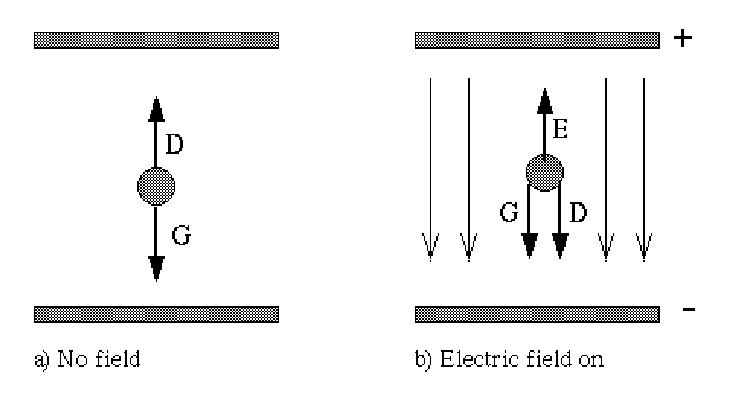
\epsfig{file=Introduction/oil_droplet.eps, height=5cm}
  \caption{
    Forces on an oil-droplet in: \newline
    \hspace*{1.5cm}
           a) Free fall          \newline
    \hspace*{1.5cm}
	   b) Electric field     \newline
    (G=Gravitation, D=Drag, E=Electric force)
  }
  \label{oil_droplet}
\end{center}
\end{figure}

His results were systematically low by about 4\% due to inaccurate
knowledge of the coefficient of viscosity. \newline
The electron charge is -e,
where $e = 1.602 \cdot 10^{-19}C$. All free particles are observed to
have values of electric charge equal to an integer times the
fundamental charge e:

\begin{equation*}
  q=n e
\end{equation*}

where the integer $n=\dots,-1,0,1,\dots$ is the electric charge
\emph{quantum number}.

\subsection*{The Nucleus}

In 1912, Ernest Rutherford and his associates discovered that the
positive charge of the atom is concentrated in a \emph{nucleus}. The
charge of the $\alpha$ particle, discovered by Becquerel, was
determined to be $2e$, and the mass of the $\alpha$ particle was
determined to be about four times the mass of the hydrogen
atom. \newline
A new particle with zero electric charge was discovered by bombarding
beryllium atoms with $\alpha$ particles. James Chadwick showed that
the new particle, the \emph{neutron}, had mass nearly equal to that of
the \emph{proton}.

\subsection*{The Bohr Model of the Atom}

In 1913, Niels Bohr made the first qunatitatively successful model of
the atom. Inspired by the work of Rutherford, Bohr made a planetary
model of the atom; with electrons moving in circular orbits about the
nucleus. This model may seem quite simple in retrospect, but for the
time it was a great advancement of science. In addition to the
classical circular orbits, the second part of Bohr's atomic model
contains a bold hypothesis of new physics. The new physics recognizes
that \emph{angular momentum} is \emph{quantized}; it can take only
certain values:

\begin{equation*}
  L = mvr = n \hbar
\end{equation*}

where $n$ is a positive integer. Solving the energy equations result
in orbits of radius:

\begin{equation*}
  r_n = \frac{n^2\hbar^2}{mke^2}
\end{equation*}

where the \emph{Bohr radius}

\begin{equation*}
  a_0 \equiv r_1 = \frac{\hbar^2}{mke^2} \approx 0.053 nm
\end{equation*}

is in the correct order of magnitude for the size of the atom!

{\bf Planc }





%               The Two First Excited states of Helium
\subsection{The Two First Excited states of Helium}

We will not make any calculations regarding exited states in this
thesis, but it is a really important issue in quantum mechanics. The
ground state energy does not tell much about the 
chemical properties of the atom on its own. Therefore good
approximations of the exited states are needed. Also, when discussing
different numerical approaches for solving the many body-problem,
including linear combinations of exited states may greatly improve
some original approximation to the ground state. Furthermore,
understanding how we include exited states is important for fully
understanding the application of the Slater determinant.
\newline
%
\newline
The state of helium with the $1s$ and the $2s$ orbitals occupied
with one electron each. 








The construction of the
periodic table in the second half of the $19^{\mathrm{th}}$ century
was based on the chemical properties of the different atoms. These
properties were not understood until the development of quantum
mechanics. The electrons are filled from the energetically lowest
orbitals. In the $s$ orbitals only two electrons of different
spins are allowed. Disregarding electron repulsion this would imply
that twice the energy is needed in removing an electron from ground
state helium than from the ground state hydrogen. This due to the 
double electric charge of the helium nucleus. The ionization energy of
hydrogen is $13.60 eV$ and the ionization energy of helium is $24.58
eV$ (ref. \cite{atkins2003}). The electron repulsion thus reduce the
ionization energy by almost $10\%$.
\newline
%
\newline
The early development of quantum theory may be summarized through the
four postulates of quantum mechanics.


%*************** The Postulates of Quantum Mechanics **************
%*
%*
\section{The Postulates of Quantum Mechanics}

A common formulation of quantum mechanics is by means of linear
algebra. In this formulation every state is represented as a (usually
infinite dimensional) complex vector, and an operator is represented
as a complex, linear and hermitian matrix. 
The postulates of quantum mechanics fall naturally into two sets: the
first three, which tell us how the system is depicted at a given time,
and the fourth, which specifies how this picture changes with time. 
\newline

%*                     The First Postulate                              *
%\subsection{The First Postulate}

{\bf \large Postulate 1}
\emph{
The state of a quantum mechanical particle is described by a vector
$\Psi$ in a Hilbert space ${\cal H}$. All the possible states of the
particle are ${\cal H}$ except the zero vector.
\newline
}

The first postulate states that a particle is described as a vector in
the Hilbert space. So a particle with finite degrees of
freedom $\mathbf{x}$ and $\mathbf{p}$ in classical
mechanics, now has infinite degrees of freedom. 
\newline

%*                     The Second Postulate                              *
%\subsection{The Second Postulate}

{\bf \large Postulate 2}
\emph{
Every observable are represented by an Hermitian linear operator in
${\cal H}$. For every classical dynamical variable
$\omega(\mathbf{x},\mathbf{p})$ there is a corresponding quantum
mechanical operator $\Omega$  obtained by operator substitution of the
fundamental position and momentum operators $\mathbf{X}$ and
$\mathbf{P}$, respectively: 
}
%
\begin{equation*}
  \Omega(\mathbf{X},\mathbf{P}) = \omega(\mathbf{x} \to
  \mathbf{X},\mathbf{p} \to \mathbf{P})
\end{equation*}
%
\emph{
The components of $\mathbf{X}$ and $\mathbf{P}$ are operators defined
through the fundamental commutation relation
}

\begin{equation*}
  \left[ X_i, P_j \right] = i \hbar \delta_{ij}
\end{equation*}

The second postulate tell us how to to move from the classical to the
quantum mechanical picture. The observables (or measurable quantities)
are defined through an operator. This operator may be obtained by
simple substitution of the position and the momentum of the
corresponding classical observable.
\newline

%*                     The Third Postulate                              *
%\subsection{The Third Postulate}

{\bf \large Postulate 3}
\emph{
The only possible values obtainable in an (ideal) measurement of an
observable $\Omega$ are its eigenvalues $\omega_n$. Each have a
probability
}
%
\begin{equation*}
  P(\omega_n) = \frac{\int \Psi^* \Phi_n }{\int \Psi^* \Psi }
\end{equation*}
%
\emph{
with $\Phi_n$ the eigenfunction corresponding to the eigenvalue
$\omega_n$. Immediately after a measurement the state collapses into
$\Phi_n$.
}
\newline

The third postulate tells what may be extracted from the quantum
mechanical picture by means of measurements. Note that the eigenvalues
may either have a continuous spectrum or be \emph{quantized}.
\newline


%*                     The Fourth Postulate                              *
%\subsection{The Fourth Postulate}

{\bf \large Postulate 4}
\emph{
The time development of the quantum state $\Psi$ is given by the time
dependent Schr\"odinger equation,
}

\begin{equation*}
  \hat{H} \Psi(\mathbf{x},t) = i\hbar \frac{\delta}{\delta
  t}\Psi(\mathbf{x},t) 
\end{equation*}

The fourth and final postulate defines the Schr\"odinger
equation. This equation describes how the quantum mechanical state
evolve in time.
\newline





\chapter{Introduction}
\thispagestyle{empty}
The complexity of the
nuclear many-body problem has made nuclear physics a field driven
by discoveries of outstanding phenomena. Tanihata's discovery in 1985 
\cite{isao} of vastly spatially
extended nuclei ($^{6,8}$He; $^{11}$Li; $^{11}$Be) at the neutron
dripline, 
triggered an interest in the study of weakly bound
and resonance phenomena in few-body systems.
With access to secondary
exotic nuclear beams, the edges of the nuclear landscape itself
are being explored, {\em i.e.} the very limits of nuclear
existence. At these limits, the so-called neutron (proton) {\em
driplines}, additional neutrons(protons) literally drip out of the
nucleus.  Nuclei far from stability
allow us to amplify and isolate particular aspects of the nuclear
interaction and dynamics. Using what we learn from these nuclei we
can then return to the nuclei of the world around us and
understand them far better than ever before. Progress in nuclear
structure is made at the various levels where one attempts to
understand nuclear phenomena; (i) Experimental data and
phenomenology, (ii) `Local models' (effective models with few
emergent degrees of freedom),
 (iii) `Global nuclear models',
(iv) Ab initio NN-interaction based procedures, (v) QCD.
There is an overall effort to explain higher levels in terms of
lower ones, but a more reductionist ``deductive approach'' is
likely to have as precursor an approach which tries to isolate and
understand the characteristic degrees of freedom. 

\section{Few-body aspects of dripline nuclei.}
 Nuclei along the dripline with 
an extreme dilute neutron skin have been labeled \emph{halo nuclei}. 
Understanding the mechanisms underlying the formation of such nuclei 
has been a theoretical challenge, especially two-neutron 
Borromean\footnote{ The three Borromean rings, the heraldic symbol of
the Italian Borromeo family, are interlocked in such a way that if
any of them were removed, the other two would also fall apart. The
three interwined Borromean rings are now widely used as the logo
of the halo field.} halos such as $^{6}$He and
$^{11}$Li. The Borromean nuclei display extreme clusterization into an
ordinary core nucleus and veil of halo nucleons -- forming
exceptionally dilute neutron matter. This clusterization  
has motivated few-body approaches such as the hyperspherical harmonic method 
and momentum space Faddeev equations,
to these nuclei \cite{zhuk}. Borromean nuclei such as $^{6}$He and $^{11}$Li 
has been especially suitable for few-body models, they are
characterized by pairwise constituents with no bound states but
modelled as a three-body system they achieve binding.
The extreme size of these dilute neutron excessive 
nuclei is mainly caused by the outermost neutrons being very loosely bound or
even unbound, causing a large tail in their wave functions.  
%\begin{wrapfigure}{r}[0pt]{5.5cm}
\begin{figure}[tb]
%\begin{center}
%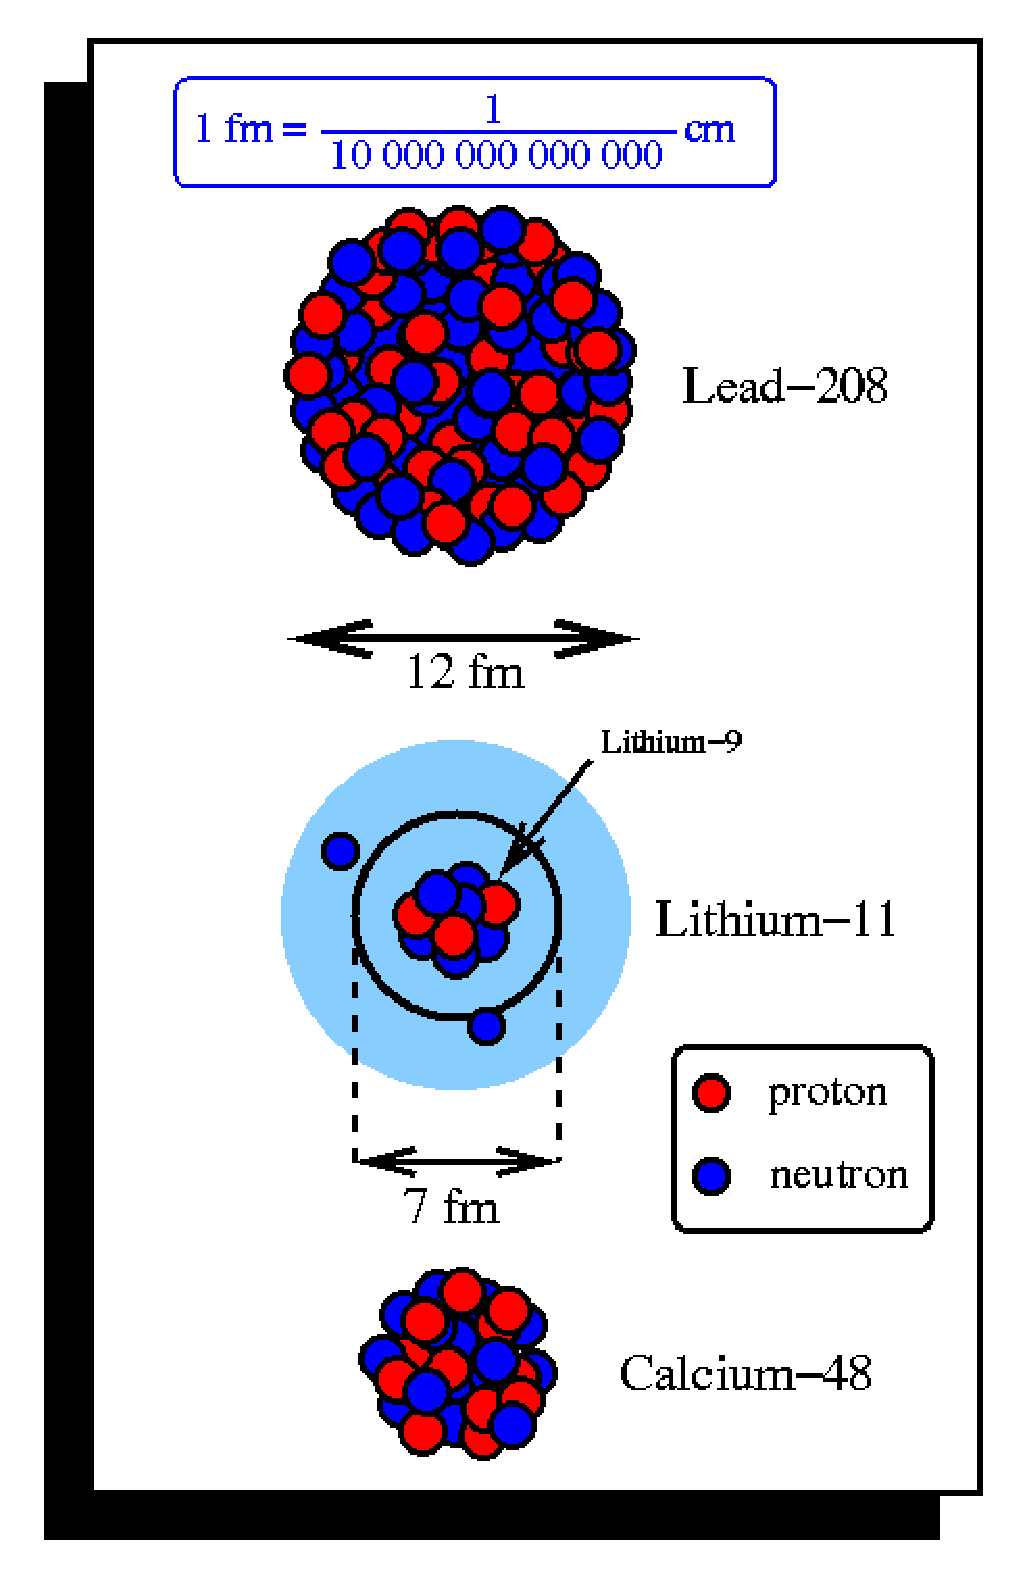
\includegraphics[scale=0.33]{lisize.eps}
%\end{center}
\centerline{\psfig{figure=figures/lisize.eps,width=8cm}}
\vspace{3mm}
\caption{The matter size of $^{11}$Li is compared to
that of $^{48}$Ca and $^{208}$Pb \label{Size} }
%\end{wrapfigure}
\end{figure}
Figure~\ref{Size} shows the spatial extension of the Borromean nuclei 
$^{11}$Li in comparison with the nuclei $^{48}$Ca and $^{208}$Pb. The spatial
extension is huge, the rms matter radius of $^{11}$Li is as large
as that of $^{48}$Ca, and the radius of the halo neutrons is as large
as for the outermost neutrons in $^{208}$Pb. 
To understand theoretically this abnormal feature of dripline nuclei 
has been a challenge over the years.


Borromean nuclei along the dripline have the property of being 
bound in their ground state. 
The ground-state properties of the Borromean nuclei $^{6}$He has been 
well understood in terms of few-body modelling \cite{zhuk}. The 
$\alpha $ core of $^6$He is stable and well bound, and it 
may be frozen in its ground state.
The relevant degrees of freedom are then described by the two halo neutrons 
relative to the core. 
In three-body models of halo nuclei such as $^6$He, Pauli blocking
is needed to remove components of the halo wave function that
would disappear under full antisymmetrization. This, and also
other aspects of the composite nature of the clusters make the
challenge somewhat different from that of three-nucleon systems.

However, most nuclei along the dripline
exhibit an unstable character, in that their ground state is embedded
in the continuum, in the form of a resonance. The hadronic stability 
of Borromean nuclei is mainly due to strong pairing effects between the 
outermost neutrons. Figure~\ref{Map} gives the hadronic
stability of various isotope chains, and it is seen that
while $^5$He is unbound $^6$He is bound, $^7$He is unbound but
$^8$He is again bound. A recent review \cite{jonson} looks at
all the dripline nuclei.
\begin{figure}[tb]
%\begin{center}
%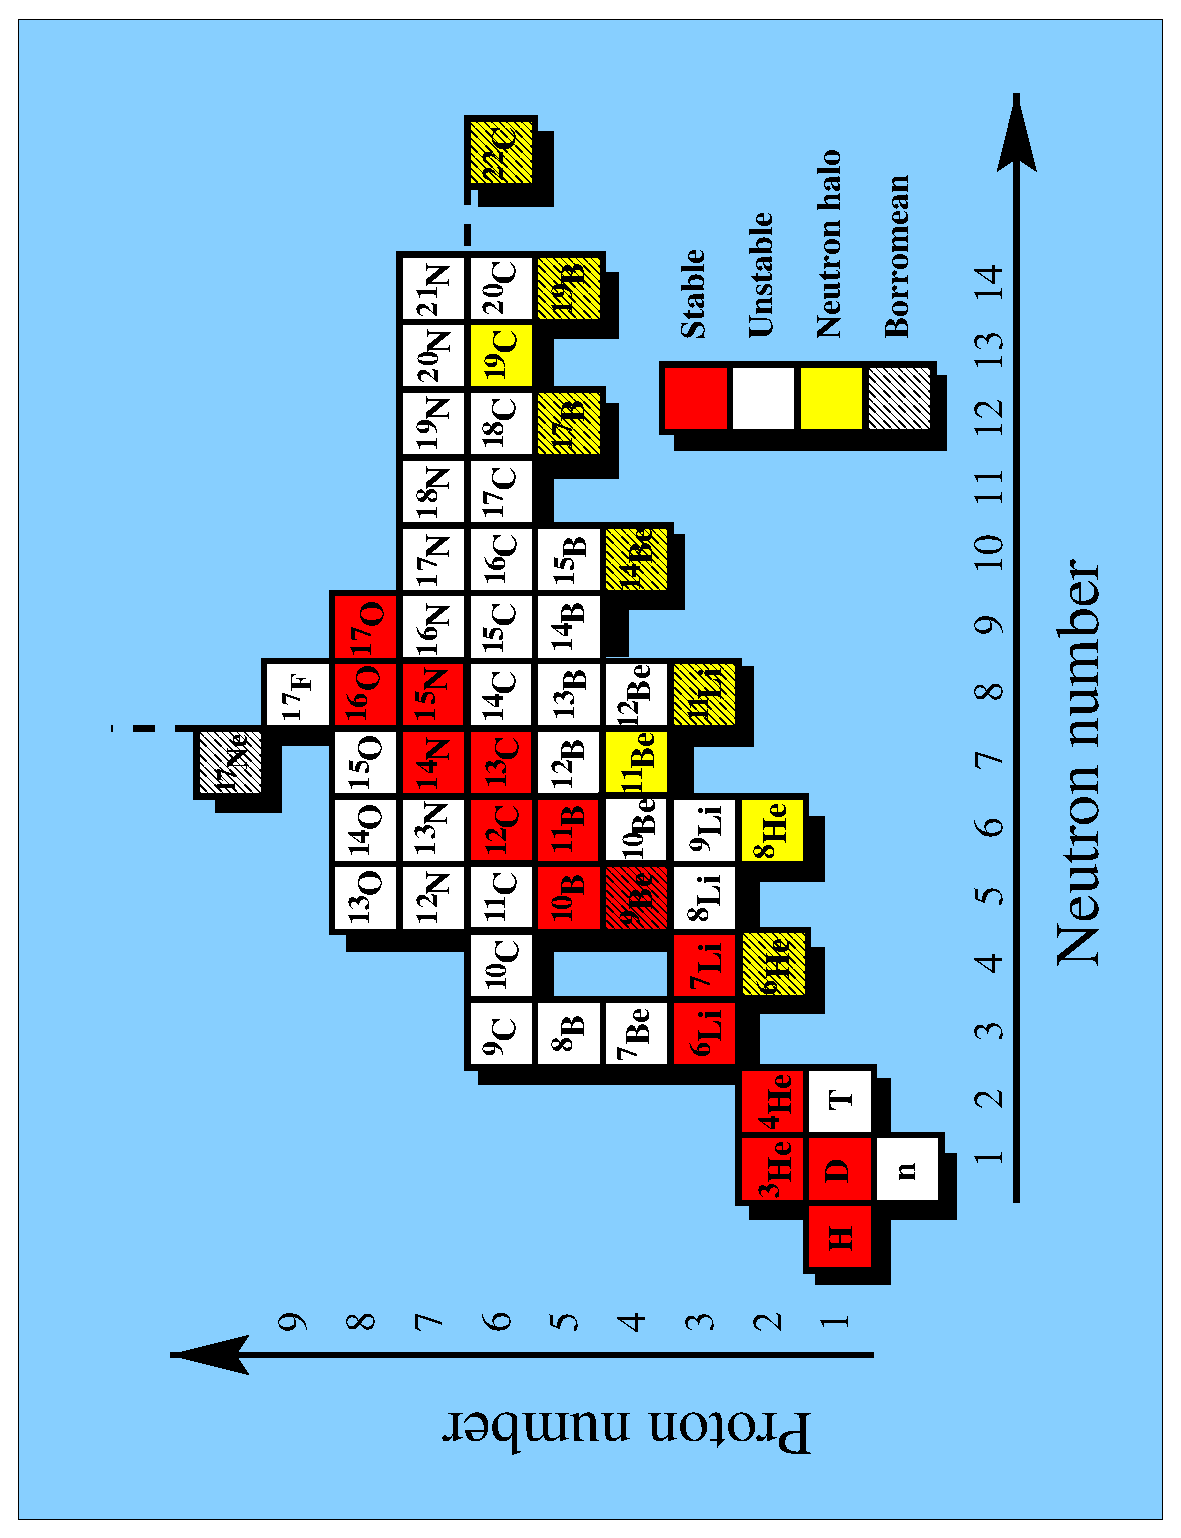
\includegraphics[scale=0.4,angle=270]{segre.eps}
%\end{center}
\centerline{\psfig{figure=figures/segre.eps,width=8cm,angle=270}}
\vspace{3mm}
\caption{The nuclear chart exhibits the stability of
Borromean nuclei among different isotope chains \label{Map}}
\end{figure}
Dripline physics, which involves nuclei  with one or a few weakly bound 
states, is physics of threshold phenomena where structure and
reaction theory merge. Hence the development of  methods for dealing with 
resonance and other continuum phenomena in such nuclei is of great importance.

\section{Resonances in quantum mechanical few-body systems.} 
The characteristic feauture of exotic states embedded in 
the continuum is that they only exist for a limited time, 
before they fall apart into their decay products. Such states are labeled quasi-stationary 
or resonant states. In a two-body picture, they may understood as states trapped inside 
the centrifugal barrier for limited time, before they tunnel through the barrier and decay.
Such resonant structures are often called \emph{shape resonances}, see figure~\ref{fig:pot_barrier}.
\begin{figure}[hbtp]
\begin{center}
\resizebox{10cm}{8cm}{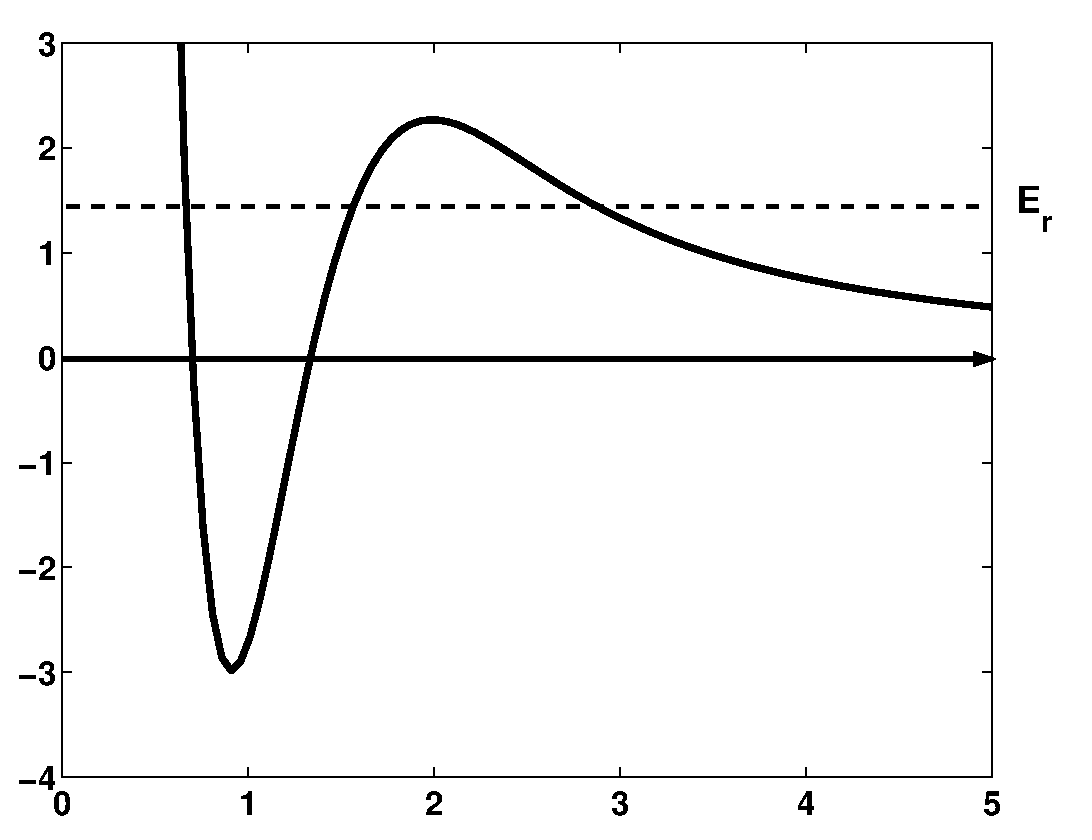
\epsfig{file=figures/pot_barrier.eps}}
\end{center}
\caption{Confining potential in which a resonant state at real energy $\mathrm{E_R}$ is formed. }
\label{fig:pot_barrier} 
\end{figure}
Considering the time dependent wave function, which satisfies the Schr\" odinger equation 
for a complex energy $z = E_R - i\Gamma /2$,
\[ 
\Psi({\bf r},t) = \Phi({\bf r})exp( -i { z\over \hbar} t),
\]
it is seen that the probability density at a point ${\bf r}$,
\[  
\vert \Psi({\bf r},t)\vert^2 = \vert \Phi({\bf r})\vert^2 exp( -i { \Gamma\over \hbar} t),
\]
decreases exponentially with time only for $ \Gamma > 0$. As already pointed out by Gamow in 1928 
in his work on radioactive decay \cite{gamow}, this wave function is the only one 
appropriate for description of resonances or quasi-stationary states. Resonances 
are observed in experiments as enhancements in the cross section when plotted
as a function of energy. In the case of isolated resonances, where the distance in energy
between the resonances exceeds their widths, and the resonaces are far from 
decay thresholds, the total cross section over the resonance peak may be parametrised 
by the Breit-Wigner formula \cite{wigner},
\[
\sigma \propto {{1\over4}\Gamma^2\over (E-E_R)^2 + {1\over 4}\Gamma^2} 
\]
A detailed analysis of such data often reveals that 
this enhancement is due to one specific partial wave. To that extent, resonances have a 
definite set of quantum numbers just like bound states, the only differences being
the fact that these states have a definite lifetime and thus correspond to 
complex energy eigenstates. Standard quantum mechanics is formulated for
Hermitian operators. This raises the question of how a Hermitian Hamiltonian 
could give rise to a complex eigenvalue and whether such states should be 
included in our Hilbert space? 

How to actually solve for single particle resonances has been a separate study 
in many different areas of quantum physics over the years.  
The specialization trend within all disciplines of 
applied quantum physics makes it almost impossible to understand 
questions and problems raised within the different branches of quantum 
physics, on the other hand a methodological unification has taken 
place in many areas. The theory of resonances is such an example.
The theory underlying the formation and decay of 
long lived states in molecules, atoms, nuclei, and condensed matter is
from a quantum mechanical viewpoint  methodologically basically the same. 
By acknowledging this, it is possible to obtain new perspectives in 
various fields by  adopting methods originally developed in
different fields of physics 
A variety of methods has been developed for understanding the basic 
mechanisms of formation of resonant states and processes taking place in the continuum.
They are described in text books such as \cite{newton, kukulin, sitenko, zeldovich}.
All the methods have in common that they originate from standard scattering theory,
and are based on the method of analytical continuation. The relevant equations are 
analytically continued from the physical energy sheet through the 
unitarity cuts onto the second energy sheet of the complex energy 
plane, where resonances may be located. 

One of the more popular methods 
during the last decades has been the complex scaling method, originally 
formulated by Aguilar, Balslev and Combes in the early 70's \cite{abc,abc1},
and developed to examine the spectrum of the Green's function on the second energy sheet. 
Later this method has been adapted in other fields
such as atomic and molecular fields to the study of resonances by complex scaling. 
In the context of complex coordinate scaling applied to quantum chemistry,
Moiseyev \cite{nimrod1,nimrod2,nimrod} developed a generalized complex variational 
principle for resonant states.
During the last decade the complex coordinate method has also been applied in nuclear physics, 
as interest in loosely bound nuclear halo systems has grown, see for 
example \cite{csoto, myo, garrido, imante} for an application to the resonant 
states of Borromean halo nuclei.
 
More recently a method based on exact differential equations for functions
closely related to the Jost functions has been developed \cite{sofianos1,sofianos2}. The
method exploits the idea of complex rotation of the coordinates, but differs from 
the traditionally used complex scaling methods using expansions and variational 
principles. The Jost function at a complex energy is obtained directly from exact equations,
and resonances are associated with zeros of the Jost function on the second energy sheet. 

Another popular approach is method based on
analytic continuation in the coupling constant (ACCC) \cite{kukulin,aoyama}.  The ACCC method
uses analytic continuation in the coupling strength of the potential instead
of the usual continuation in energy. All these methods are usually formulated in 
coordinate represenation. 

One of the disadvantages
of the coordinate space approach is that the boundary conditions have to be 
built into the equations, and convergence may be slow if the basis does not 
mirror the physical outgoing boundary conditions well. 
Instead, it is possible to represent the Schr\"odinger equation 
in momentum representation, invoking the Fourier transform. One 
of the most obvious advantages of this, is that the boundary conditions for 
bound and resonant states are automatically built into the transformed integral equations.
Diagonalizing, using a plane wave basis is very accurate \cite{hagen}, since the 
convergence is only governed by the number of integration points.

As shown by Afnan \cite{afnan1} a rotation of the integration contour in the 
lower half complex $k$-plane is equivalent to the complex coordinate rotation
method, and in this respect the coordinate and momentum space versions are complementary.
It should be mentioned that  
the contour deformation method (CDM) formulated \emph{in momentum space} is not new
in nuclear physics. It was studied and applied in the 1960`s  and 1970`s,  
see for example \cite{brayshaw,nuttal,stelbovics,glockle}, especially in the field of 
three-body systems. Most of these references
applied a \emph{contour rotation} in momentum space. By restricting 
oneself to a rotated contour certain limitations and restrictions however appear in the
equations, determined by the analytical structure of the integral kernels and potentials. 
In \cite{glockle} a more sophisticated choice of contour, 
based on rotation and translation, 
was applied to the three-nucleon momentum space Faddeev equation for a separable Yamaguchi interaction.
This choice of contour made it possible to avoid the logarithmic singularities of the Faddeev kernel
and hence allowed for a continuation in energy to the non-physical energy sheet. 
The method has recently been revived to study anti-bound and resonant 
states in subatomic physics \cite{hagen}, where a general contour was considered.

The question now arises, whether resonant states can be made part
of a complete set of states, appropriate for eigenfunction expansions. 
In the late 60's Berggren proved that for a finite range potential, 
a finite set of bound and resonant states together with a set of 
non-resonant continuum states form a complete set \cite{berggren}
of bi-orthogonal functions. 
\begin{equation}
{\bf 1} = \sum _{n}\vert\psi_{nl}\rangle\langle\psi_{nl}\vert + 
\int_{L^+} dk k^2\vert\psi_{l}(k)\rangle\langle\psi_{l}(k)\vert,   
\label{eq:berggren1}
\end{equation}
this representation has later become known as the \emph{Berggren basis}.
The non-resonant continuum integral is defined along a contour in the 
in the fourth quadrant of the complex $k$-plane, and the discrete sum is over 
both bound and resonant states. 

In this representation the usual inner-product is no longer Hermitian. 
The resonant states are not normalizable in the usual sense, as they 
oscillate and diverge exponentially along the real axis. 
As first shown by Zel'dovich \cite{zeldovich}, the inner product of
a resonant state together with its complex conjugate, may be given a definite 
value by some reguarlization procedure. 
Expanding the scattering and reaction amplitudes in this basis, makes
it possible to separate the resonance behaviour from the smooth non-resonant 
background in the scattering amplitudes. This is motivated by the 
fact that the most interesting phenomena taking place in the continuum 
are the resonance phenomena. 


\section{Modern \emph{Ab initio} approaches to nuclear structure.}
In physics one often attacks a specific problem within a reductionist way of thinking. 
That is, the phenomena of the whole system 
should be described in terms of the theories and laws of the parts of the system. 

In nuclear physics one would ideally like to start from nucleon degrees of freedom.
The dominant philosophy within the nuclear theory community is 
that the nucleus (at low energies) as a whole  may be fully described in terms of the 
the interactions between these constituents.
Building up the nucleus from these basic constituents and their mutual interactions, 
the quantum mechanical description of the many-body system however becomes extremely 
complex and hard to tackle as the number of nucleons increases. 

In the history of nuclear structure the shell model has been very
successful in describing properties of nuclei near the valley of stability.
The traditional shell model has usually been formulated in a harmonic oscillator 
representation, this is based on the assumption that 
the single particle motion within the nucleus is well described by harmonic oscillator orbitals.
This is certainly true for well bound nuclei where the tail of the single particle
wave functions fall of rapidly.
The harmonic oscillator wave functions are also favourable as
they are given in terms of well known mathematical functions. However, the possibly most attractive aspect is
that the Hamiltonian describing the motion of two particles in a harmonic oscillator potential may 
be written in separable form in both relative and center-of-mass coordinates and 
shell model coordinates. This is extremely favourable since the 
effective interaction between the nucleons are given in relative coordinates.

The shell model approaches to nuclear structure are usually not 
truely reductionistic. For heavier nuclei the number of degrees of freedom becomes 
too large to handle with modern computers. Therefore it has been customary 
to define an inert core of the nucleus which sets up a mean-field in which 
the valence nucleons move. Thus the nucleus $^{18}$O may be modelled 
with two valence nucleons moving in the $s-d$ shell with respect 
to the closed shell nucleus $^{16}$O acting as an inert core. 
As the number of valence particles grows the number of nucleon configurations 
within a valence space becomes larger and larger, making it diffucult 
to handle numerically. 
Nevertheless, in the last decade one has experienced an extreme 
development of computational power, making it possible to extend the shell model
into regions previously inaccessible. 

The growth of computational power has also sparkled a belief 
in \emph{ab initio} calculations of nuclei, taking into account all 
degrees of freedom. The most ambitious of these `reductionist' attempts are Green's
Function Monte Carlo (GFMC) calculations \cite{pieper1,pieper2,pieper3,pieper4,pieper5,pieper6,pieper7}, 
extending previous variational Monte Carlo (VMC). According to the authors
these are the first microscopic calculations that directly
produce nuclear shell structure from realistic interactions that
fit NN scattering data. Another line of approach are the
large-basis no-core shell-model (NCSM) calculations of Barrett's
group \cite{bruce1,bruce2,bruce3,bruce4}, where the shell model is combined with
microscopic effective interactions derived from modern
nucleon-nucleon potentials. 

The exponential growth of the configuration space as the number of
active particles increases makes it extremely difficult to reach 
into the range of medium size nuclei, within these \emph{ab intio} 
formalisms. The cost of matrix diagonalization increases as the third power
of the number of basis states, and the memory required to store the 
Hamiltonian matrix increases as the square of the number of basis states.
The practitioners have, however, already had success with their
pioneering attempts. So far converged results for nuclei with up to $A = 12$ 
active particles have been reported. Further, GFMC and NCSM calculations 
for A=6 do produce an alpha-like core object, and two alpha-particles for $^8$Be,
both promising features.

Another \emph{ab initio}�
approach which recently has proved promising in the 
medium size region of the nuclear chart, is the Coupled-Cluster method.  
The Coupled-Cluster method originated in nuclear physics in the 60's 
\cite{cc4,cc5}, but has since that time only appeared sporadic within 
nuclear physics. On the other hand Coupled-Cluster theory has 
been extensively used, and with great success, 
in quantum chemistry over the years \cite{cc6,cc7}. 
Basically the Coupled-Cluster method  is based on an 
exponential ansatz for describing correlations within a nucleus. 
\[ 
\Psi_{CC} = exp(\hat{T})\Psi_0, \:\: \hat{T}�= \hat{T_1} + \hat{T_2} + \hat{T_3} +...,
\] 
where $\hat{T}_n$ are linear combinations of all $n$-type excitations. 
Including only single and double excitations (CCSD), the computational cost 
scales as $ N^7$�where $N$ is the size of the system. Instead of direct matrix
diagonalization, a non-linear set of equations is solved iteratively. 
Very recently \cite{cc1,cc2,cc3}, converged Coupled-Cluster 
results for the ground- and first excited state of $^{16}$O have been reported, using 
modern nucleon-nucleon interactions derived from effective field-theory.

\section{Exotic many-body states embedded in a continuum.}
All of the above mentioned many-body approaches have been formulated using 
a harmonic oscillator basis describing single particle motion. 
Adopting a harmonic oscillator picture, one assumes from the very 
start that the interacting nucleons are isolated from an external environment
of positive scattering states. The tremendous success of the multi-configurational 
shell model over the second part of the last century, in describing properties of nuclei
where continuum aspects are more or less absent, has given little focus on mechanisms 
involved in the formation and decay of nuclei far away from the valley of $beta$-stability. 
However, approacing the drip-lines
new aspects and properties of nuclei emerge, such as the instability of decay, enormous size 
of halo nuclei and the melt down of shell structures and new shell closures. 

To bridge the gap between reaction and structure theory,
microscopical shell model calculations using a Berggren representation for the
single particle states were proposed some years ago \cite{lind,liotta}. 
The proximity of the scattering continuum in weakly bound and unbound nuclei,
implies that these nuclei cannot be properly described without taking into 
account the coupling between discrete states and   the 
positive energy continuum. In other words, a proper description of loosely bound 
nuclei should take into account the coupling of the internal with the external 
environment, which has been totally neglected in classic shell model approaches.
The coupling of the 'external' continuum of positive energy states, with the 'internal' 
nuclear states has for a long time been basic ingredient in nuclear reaction theory. 
Feshbach was the first to formulate a unified description of direct and 
compound nuclear reactions within the projection operator method \cite{feshbach1,feshbach2}. �
He showed that the coupling of the internal with the external environments could 
give rise to compound nuclear states, such as 
multi-channel resonances. As he was the first to 
formulate a general theory of such states, they became known as Feshbach resonances. 
Also in atomic physics Feshbach resonances
are of great importance. In the early 60's, at the same time of Feshbach's work, Fano \cite{fano} 
discussed how the mixing of a configuration 
belonging to a discrete spectrum with configurations belonging to a continuous spectrum
gives rise to the phenomena of \emph{autoionization}, which is considered a multi-channel 
resonance or in other words a Feshbach resonance.

Entering the realm of weakly bound nuclei, it becomes evident that the 
standard separation of nuclear structure and nuclear reaction methods has
to be abdoned. A merging of the two fields, where many-body methods from the 
structure community are united with reaction theory, where the importance of the
continuum has been studied over several years, seems to be a fruitful way of approach.
Treating the continuum aspects properly within existing many-body theories, 
is however much more difficult than when dealing with well bound nuclei.
Existing many-body structure approaches have to be reformulated and developed further since 
the harmonic oscillator representation has to be abdoned. 
All the nice 
mathematical properties of the harmonic oscillator basis are non-existent 
in all other single particle representations, e.g. the Woods-Saxon basis. 

Having determined a single particle basis consisting of bound, resonant and 
non-resonant continuum states, it is natural to again focus on the 
application of this basis in nuclear structure calculations of weakly bound and/or 
unbound nuclei. Ideally one would like an \emph{ab intio} description
of these nuclei, taking into account all relevant degrees of freedom. In the 
hyperspherical description of three-body Borromean and halo nuclei, 
the problem of treating core excitations and the anti-symmetrization between core and valence 
nucleons has not fully been solved. Treating such nuclei microscopically, a reformulation 
of the shell model using a single particle basis of bound, resonant and scattering states 
may appear to be the most straightforward method. 
The recently developed Shell Model Embedded in the Continuum (SMEC), see e.g.  
Refs.~\cite{csm1,csm2,csm3,vz2003}, offers such a possibility. 
SMEC is closely related to the Feshbach projection operator technique. 
In SMEC the bound,resonant and scattering states are treated on equal footing,
by introducing two subspaces and taking their coupling into account.
However, most SMEC calculations have not taken into account coupling with decay channels  
containing more than one nucleon. 

Restricting the theory to only one-nucleon 
decay channels, limits the applicability of SMEC along the drip-lines. Borromean 
nuclei for which the $A$�and $A-2$ nuclei are particle stable, while the nuclei $A-1$ are not, 
requires a theoretical description which takes into account decay channels involving all valence 
nucleons. That is, all many body configurations involving bound and scattering states should 
be considered. 
The newly developed Gamow shell model is devoted to such an approach, see for example 
Refs.~\cite{michel1,michel2,michel3,liotta,betan,witek1,witek2,roberto,betan2,hagen}.
The Gamow shell model starts with the Berggren representation (\ref{eq:berggren1}) for single particle states. 
A complete many-body Berggren basis may then be constructed from the 
discretized single-particle Berggren orbitals
\[ 
\sum_n \vert \Psi_n\rangle \langle \tilde{\Psi}_n\vert = 1,
\]
where the many body Slater determinants $\vert \Psi_n\rangle $�are constructed 
from the discrete bound, resonant and non-resonant continuum orbitals.
This is in full analogy with the standard shell model 
using a harmonic oscillator basis.  
When the exact multi-particle resonance wave function is expanded in a complete 
set of Slater determinants consisting of discretized single particle Berggren 
orbitals,  an interpretation of these exotic multi-particle structures
in terms of single particle resonances becomes possible. 

Intuitively one would expect that the 
Slater determinant built from single-particle resonances only, would be the
major component in the fully correlated many body wave function. This is certainly true
if the residual nucleon-nucleon interaction is weak compared with the 
mean-field in which the valence particles move. More interesting is the opposite
case, where the residual interaction is strong. In this case it is not 
obvious that the pure pole configurations are the most important. However, 
the Gamow shell model may provide an answer to the question of how exotic 
structures, such as multi-particle resonances, embedded in the continuum are formed.
The Gamow shell model is a promising many-body approach in the study of unstable nuclei
along the drip-lines. And it is in the unifying spirit of scientific development, in that it
reconciles the reaction and the structure part of the community. 
The Gamow shell model is in its early stages, and so there exist  a vast 
area of applications and mayor theoretical and computational challenges to be dealt with.
One of the first challenges and problems encountered in the Gamow shell model, was
the \emph{identification problem}, and first addressed in \cite{liotta, betan}.
The physical multi-particle resonances 
will in many cases be embedded in a dense distribution of continuum states, 
depending on the contour on which the continuum states are defined.  
Refs.~\cite{liotta, betan} related this \emph{identification problem} to 
the problem of choosing a contour in the complex $k$-plane which 
in the case of several valence particles selects the physical interesting
states from the dense continuum background. They found that in the two-particle
case, choosing a \emph{square-well} contour makes an identification 
of physical states based on 
inspection of the zeroth order energy surface possible. This solution is
only  applicable in the two-particle case,  already in the tree-particle case
the physical states get mixed in with the continuum states.
In Refs.~\cite{michel2,witek1,witek2} the problem of identifying multi-particle 
resonances was approached from a different angle.
The proposed algorithm is a two step procedure. In the first step 
a diagonalization within the pole space, where all particles are in 
resonant single particle orbitals, is performed. Secondly a 
diagonalization within the complete configuration space is done.
Under the assumption of weak coupling of the pole configurations
with the configurations where at least one particle moves in a continuum orbital, 
the physical states may be picked out unambiguously from the states obtained after a 
full diagonalization, using the criterion of largest overlap with the pole space.
The weak coupling limit may not always be a valid assumption, as pointed out in Ref.\cite{betan2} 
for the case of $^{11}$Li the two-particle resonances may
have a larger continuum component as compared to the pole component,
depending on the strength of the residual nucleon-nucleon interaction.
Presently one may conclude that the \emph{identification problem} has not
been solved generally, and developing an algorithm which picks out 
physical states unambiguously from the dense continuum background is still an open problem.

Another challenge for the Gamow shell model is the \emph{dimensionality problem}. As the number
of active particles moving in a valence space increases, the 
number of Slater determinants in the many-body Berggren basis increases dramatically. 
This explosion of many-body configurations is  even more severe than in the 
standard shell model approach where only bound states appear. In the Gamow shell model
one has for each partial wave a finite number of non-resonant continuum states which are absent
in the standard shell model. In solving this problem, one has to take advantage of 
effective operator and perturbation method techniques 
typically used and developed for large scale shell model 
calculations using harmonic oscillator bases. 

With further progress in computational power   
one may hope that \emph{ab intio}  calculations of light and medium 
size nuclei within the Berggren representation may become possible in the near future. 
Coupled-Cluster techniques has proven to be a promising method for 
microscopical calculations of medium size nuclei such as
$^{16}$O,
a promising way of approach would be 
to generalize the Coupled-Cluster method to complex interactions, and
at the first stage see how resonant structures are formed in light nuclei
starting from an  \emph{ab initio} approach. Another interesting application 
would be to see how single particle resonances are formed starting from 
a realistic nucleon-nucleon interaction. In conclusion, one may say that 
nuclear physicists are living in exciting times.


\section{Outline of Thesis.}
This thesis combines results which are published in 
international journals with 
results which appear only in this thesis. 
The main purpose of this thesis, may 
nevertheless be summarized in the two published papers   
{\it The contour deformation method in momentum space, 
applied to subatomic physics}  and 
{ \it Effective Interaction 
Techniques for the Gamow Shell Model}. However, since
these papers deal with topics which may be less familiar to 
the audience, this thesis aims at giving 
a more detailed and thorough discussion of the formalisms and theories
underlying this work. The outline of the thesis is the following. 

Chapter~2 gives a detailed discussion of the scattering functions
and Jost functions starting with the coordinate representation 
of the Schr\"odinger equation.  The most general distribution of 
poles of the scattering matrix is discussed, together with their 
physical interpretations. Chapter~2 also dicusses some 
typical regularization procedures for matrix elements involving 
resonant states. An outline of the proof of the general 
Berggren completeness which includes bound, anti-bound and resonant
states is given, and a discussion of the physical 
interpretation of expectation values of observable operators
involving resonant states.

Chapter~3 starts with the momentum representation of the 
Schr\"odinger equation (Section~\ref{sec:momspace}), 
and discusses how the Schr\"odinger equation 
may be analytically continued to the second energy sheet using 
the Contour Deformation Method (CDM) 
(Section~\ref{sec:analytic_continuation}).
A complete set of 
single particle states, involving all kinds of poles, 
is obtained. Chapter~3 contains several applications
which are not included in the published papers. 
Section~\ref{sec:deformed} gives an application of the CDM to the 
problem of solving for resonances in a deformed field is given 
Section~\ref{sec:optical} gives an application of CDM to 
resonances and bound states in complex absorbtive and emitting 
potentials.
Section~\ref{sec:inmedium} gives an application of CDM 
to the solution of pair instabilities of the CD-Bonn interaciton 
in a infinite nuclear medium, and discusses how 
poles on the second energy sheet may be interpreted as resonance
like states. 


Chapter~4 discusses the application of a single-particle
basis constructed by CDM may serve as a starting point
for Gamow-Shell-Model studies. Section~\ref{sec:lanczo}�
discusses how the Lanczos iteration method may be applied to 
the calculation of multi-particle resonances in the Gamow Shell
Model formulation. As numerical test study, the convergence
of the $0^+$ ground state and the $2^+$ resonance energy of 
$^6$He for each iteration is given. The results are promising for
large-scale Gamow Shell Model calculations. 
Section~\ref{sec:lee_suzuki}
gives a formal derivation of the Lee-Suzuki similarity
transformation method for complex interactions, and shows 
how a complex symmetric interaction may be obtained 
by a second similarity transformation. Section~\ref{sec:multi_reference}
discusses the use of Many-Body perturbation theory in 
Gamow-Shell-Model calculations. A derivation of the standard
Rayleig-Schr\"odinger perturbation expansion for 
a single model space state is given for the case of complex
interactions. It is shown that the standard single-reference
perturbation theory does not give satisfactory results
when treating many-body resonance perturbatively. The
Multi-Reference-Perturbation-Theory-Method (MRPTM) is
subsequently derived. This theory differs from 
standard perturbation theory, in that it is a  
one-state-at-a-time perturbation theory. Finally, 
Section~\ref{sec:effective_scheme} gives an effective
interaction scheme for the Gamow-Shell-Model 
which combines the Lee-Suzuki similarity 
transformation method with the one-state-at-a-time MRPTM. 

Chapter~5 gives a short introduction to the 
article {\it The contour deformation method 
in momentum space, applied to subatomic physics}. 

Chapter~6 gives a short introduction to the 
article { \it Effective Interaction Techniques for the Gamow Shell Model}.

In Chapter~7 conclusions of the present work, and future 
perspectives are given.  



 
 




% shell model embedded in the continuum. 







% label{eq:chap21_eq1}
\chapter{General theory of resonances and the Berggren completeness.}
\label{chap:gentheory}

\section{Physical interpretation of scattering matrix poles.}
\label{sec:physical_interpretation}  
Resonance phenomena are associated with processes taking
place in the continuum. Any quantum mechanical system may 
be experimentally found to be either in a bound stationary 
state or in a scattering state located in the positive continuum.
Resonance states with definite lifetime are never directly observed, 
but instead the scattering states into which they decay are observed. 
It is therefore natural to start with the radial Schr\"odinger equation,
for a spherically symmetric potential $V(r)$,
\begin{equation}
  \left( -{d^2\over dr^2} + v(r) + {l(l+1)\over r^2} -k^2\right) u_l(k,r) = 0
  \label{eq:chap21_eq1}
\end{equation}
here $v(r) =  2\mu V(r)/ \hbar^2  $ and the energy is related to the 
wavenumber by $k^2 =  2\mu E / \hbar^2 $, where $\mu$ is the 
reduced mass of the system. There are four different types of 
physical states associated with this Schr\"odinger equation,
bound, anti-bound, resonant and scattering states, differing in 
the boundary conditions imposed on the wave functions at large
distances. 

In the following an overview of the properties of the 
regular and irregular solutions of the Schr\"odinger equation, and
their relation to the physical scattering wave function is given. For 
a more detailed review the reader is referred to the text books 
of Newton \cite{newton} or Sitenko \cite{sitenko} on scattering theory.

Next we assume that the central potential is less singular near the origin than $r^{-2}$
and vanishes faster than $r$ at infinity, that is,
\begin{equation}
  \mathop{\lim}_{r\rightarrow 0} r^2V(r) = 0, \:\: 
  \mathop{\lim}_{r\rightarrow \infty } r V(r) = 0.
\end{equation}
From the theory of ordinary second order differential equations 
the condition that the potential $V(r)$ has a ``weaker'' singularity than $r^{-2}$� 
at the origin, means that the point $r=0$ is a \emph{regular singular point}.
It is customary to label those solutions of equation~(\ref{eq:chap21_eq1}) which 
vanish $r=0$ \emph{regular} and those which do not \emph{irregular}�
solutions. The regular $ \phi_l(k,r) $ and  irregular solutions 
$f_l(k,r)$ to equation~(\ref{eq:chap21_eq1}), are uniquely defined by 
the boundary conditions,
\begin{eqnarray}
  \nonumber
  \mathop{\lim}_{r\rightarrow 0} (2l+1)!!r^{-l-1}\phi_l(k,r) = 1, \\
  \mathop{\lim}_{r\rightarrow \infty }\exp(ikr)f_l(k,r) = i^l. 
  \label{eq:boundary}
\end{eqnarray}
The irregular solutions $f_l(k,r) $ are called the Jost solutions, and 
from the boundary condition it follows that they have the
asymptotic form 
\begin{equation}
  f_l(k,r) \rightarrow \exp(-ikr),\:\: r \rightarrow \infty
\end{equation}
The Jost solutions $f_l(k,r)$ and $f_l(-k,r)$ are linearly independent 
solutions of equation~(\ref{eq:chap21_eq1}). This follows from the 
fact that the Wronskian of $f_l(k,r)$ and $f_l(-k,r)$ is non-vanishing,
\begin{equation} 
  W\left[ f_l(k,r),f_l(-k,r)\right] = 2ik,
\end{equation}
which is easily shown using the asymptotic forms 
of the Jost solutions as $r\rightarrow \infty$. Since $f_l(k,r)$ and
$f_l(-k,r)$ are linearly independent solutions, the regular solutions 
$\phi_l(k,r) $ may be expressed as a linear combination of the Jost solutions. 
The coefficients of  $f_l(k,r)$ and $f_l(-k,r)$ are determined from 
the boundary conditions imposed on the regular solutions $\phi_l(k,r)$ at $r=0$, 
and it follows that
\begin{equation}
  \phi_l(k,r) = {1\over2} ik^{-l-1}\left[ f_l(-k)f_l(k,r) - (-1)^lf_l(k)f_l(-k,r)\right].
  \label{eq:regular}
\end{equation}
Here the Jost functions $ f_l(k) = f_l(k,r=0)$ and $ f_l(-k) = f_l(-k,r=0)$
have been introduced, and they are given by the Wronskian 
\begin{equation}
  f_l(k) = k^l W\left[ f_l(k,r),\phi_l(k,r)\right],
\end{equation}
which follows directly from equation~(\ref{eq:regular}). 
It can be shown \cite{newton, sitenko} that the regular function $\phi_l(k,r)$
is an entire function in the complex $k$-plane, while the irregular Jost solution 
$f_l(k,r)$ is an analytic function in the lower half complex $k$-plane.
From the boundary conditions in equation~(\ref{eq:boundary}) it follows 
for complex $k$ that the regular and irregular solutions satisfy the 
following conditions,
\begin{equation}
  \phi_l(k,r) = \phi_l^*(k^*,r), \:\: f_l(k,r) = f_l^*(-k^*,r). 
  \label{eq:symmetry}
\end{equation}
Further the regular solutions satisfy 
\begin{equation}
  \phi_l(k,r) = \phi_l(-k,r), 
\end{equation}
since the $\phi_l(k,r)$ is an everywhere regular function of $k^2$.

The physical scattering solutions $ u_l(k,r) $�
of equation~(\ref{eq:chap21_eq1})�are given for a mixed set
of boundary conditions, regularity at $r=0$ and the asymptotic behaviour of scattering 
wave functions as $r\rightarrow \infty$ \cite{newton}, i.e.
\begin{equation}
  u_l(k,r) \mathop{\longrightarrow}_{r\rightarrow \infty}  
  \sqrt{1\over 2\pi}i \left\{ e^{-ikr} - (-1)^l S_l(k) e^{ikr}\right\} 
  \label{eq:chap21_eq6}
\end{equation}
Here $S_l(k)$ is the partial wave scattering matrix element, which 
determines the phase shift of the outgoing wave at inifinity.
Since all physical solutions are regular at the origin, they differ from the
regular solutions $\phi_l(k,r)$ only by a normalization constant. However, 
different asymptotic behaviours of the regular solutions are specified at
specific points on the complex $k$-plane. The proper boundary 
conditions for physical states are only given at certain points in the complex $k$-plane.
If the regular solution $\phi_l(k,r)$ is
known in the entire complex $k$-plane, all physical states is in principle known.     
From equation~(\ref{eq:regular}) it follows that the asymptotic form of the regular 
solutions is given by 
\begin{equation}
  \phi_l(k,r) \mathop{\longrightarrow}_{r\rightarrow \infty} 
      {1\over2} ik^{-l-1}f_l(-k)\left\{ e^{-ikr} - (-1)^l {f_l(k)\over f_l(-k)} e^{ikr} \right\}.
\end{equation}
Comparing with equation~(\ref{eq:chap21_eq6}) it is easily seen that 
the partial wave $S$-matrix element, $S_l(k)$, is given in terms
of the Jost functions 
\begin{equation}
  S_l(k) = {f_l(k)\over f_l(-k)}.
  \label{eq:chap21_eq7}
\end{equation}
Comparing the asymptotics of the physical wave function  with the 
asymptotics of the regular solution $\phi_l(k,r)  $, 
the  physical scattering function may be written
in terms of the regular solution $\phi_l(k,r) $ and the Jost function $f_l(k)$,
\begin{equation}
  u_l(k,r) = \sqrt{2\over \pi} {k^{l+1}\phi_l(k,r)\over f_l(-k)},
  \label{eq:chap21_eq8}
  %\label{eq:chap21_eq8}
\end{equation}
which is delta-function normalized. 

Knowing all analytic properties of the Jost functions, all analytic properties 
of $S_l(k)$ follow directly.  From the definition of $S_l(k)$ given in equation~(\ref{eq:chap21_eq7})
follows that  
\begin{equation}
  S_l(-k) = S_l^{-1}(k),
  \label{eq:sym1}
\end{equation}
and from the symmetry 
property of the Jost functions given in equation~(\ref{eq:symmetry}) 
follows that
\begin{equation}
  S_l^*(k^*) = S_l^{-1}(k),
  \label{eq:sym2}
\end{equation}
where the latter property coincides with the unitarity condition for the scattering matrix 
for real values of $k$. Further, these properties establish a one-to-one correspondence 
between values of the scattering matrix in different quadrants of complex 
$k$-plane. Say that we know the value of scattering matrix at a point in the
fourth quadrant of the complex $k$-plane, $S_l(k) = {S}$. Then it
follows immediately from equation~(\ref{eq:sym1}) that $S_l(-k) = {S}^{-1}$, and 
from equation~(\ref{eq:sym2}) $ S_l(-k^*) = {S}^*$. Using again 
the symmetry relation in equation~(\ref{eq:sym1}) it finally follows
$S_l(k^*) = S_l^{-1}(-k^*)  = {S}^{-1}$. This shows that 
knowing the values of $S_l(k)$ in one quadrant of the complex $k$-plane,
the scattering matrix is automatically known in the whole complex $k$-plane.

The scattering wave function and the $S-$ matrix element $S_l(k)$ 
have poles at the same location in the complex $k$-plane, 
given by the zeroes $k = k_n$� of the Jost function $f_l(-k) = 0$. 
Due to the symmetry of the Jost functions given in equation~(\ref{eq:symmetry}), 
for each pole $k = k_n$ there is in addition a pole located at $ k = -k_n^*$. 
Furthermore the symmetry property in equation~(\ref{eq:sym1}) of $S_l(k)$ implies that for each pole $k =k_n$ 
of $S_l(k)$, it has a zero at $k=-k_n$. 
The poles in the complex $k$-plane are divided into four categories 
depending on their location in the $k$-plane, 
and are often labeled by the letters $a-d$. Consider first the case where $S_l(k)$ has
a zero for $k=-i\kappa $ for real $\kappa > 0$. Then both the regular solutions $\phi_l(k,r)$
and the physical wave functions $u_l(k,r)$ are square integrable functions since 
they fall off exponentially as $ \exp(-\kappa r)$. Furthermore the corresponding 
energy is real and negative $E = -\hbar \kappa^2/2\mu$ corresponding to a bound state
of the system. It can be shown that 
in the upper half-plane the scattering matrix $S_l(k)$ can have poles only
on the imaginary axis \cite{sitenko}. These poles correspond to the boundary conditions 
of bound states at infinity, i.e. belonging to the $\mathrm{L}^2$�functional space, with 
exponentially decaying tails, and are labeled $b$. In the lower half-plane 
the it can be shown that the poles can be positioned anywhere. 

Poles located in the fourth quadrant 
of the complex $k$-plane are associated with resonant states with outgoing 
boundary conditions at infinity, often called \emph{decaying} resonances, labeled $d$. 
To see that they correspond to outgoing asymptotics consider the regular function
in equation~(\ref{eq:regular}) at a pole of the scattering matrix,
\begin{equation}
  \phi_l(k_n,r) = \mathop{\longrightarrow}_{r\rightarrow \infty} 
      {-1\over2} (-1)^l ik^{-l-1}f_l(k_n)e^{ik_n r}
      \label{eq:asymp}
\end{equation}
A pole $k=k_n=k_1 - ik_2$ in the fourth quadrant of the
complex $k$-plane gives the specific asymptotics
\[ 
\phi_l(k_n,r) \rightarrow e ^{ik_1 r} e^{k_2 r}
\]
where $k_1,k_2 > 0$. This shows that the decay resonances correspond to outgoing 
asymptotics, furthermore they are not square integrable in the normal sense since
they are exponentially increasing and oscillating functions. 
The energy of the decay states is written in the form 
\begin{equation}
  E_n  = \mathcal{E} -i {\Gamma \over 2\mu } = 
  {\hbar^2 \over 2\mu}\left( ( k_1^2 - k_2^2) - i2k_1 k_2 \right).
  \label{eq:chap21_eq12}
\end{equation}
where the pole in the complex $k-$ plane is written 
$k_n = k_1 - ik_2$, where $k_1,k_2 > 0 $. \emph{Proper} physical resonances are 
often defined as poles where $ k_1 > k_2 $, where it is 
seen that the real part of the energy given in equation~(\ref{eq:chap21_eq12})
is positive. For poles where $k_2 > k_1$  the real part becomes negative 
and they are often called \emph{unphysical} poles.
The most interesting resonances physically, are the resonances which 
show up as sharp peaks in the cross sections, and this occurs for 
$ \Gamma \ll \mathcal{E}$. For resonance poles where the width $\Gamma $ is 
large, the resonance contribution to the cross section
tends to get smeared out within the continuum background.

For each pole located in the fourth quadrant there is a pole in the 
third quadrant symmetrically situated about the imaginary $k$- axis, these
poles corresponds to resonant states with incoming boundary conditions 
at infinity, often called \emph{capture} resonances, labeled $c$. That they are
incoming waves is seen from equation~(\ref{eq:asymp}),
\[ 
\phi_l(k_n,r) \rightarrow e ^{-ik_1 r} e^{k_2 r}, \:\:k_1 > 0,\: k_2 > 0,
 \]
Poles located on the
imaginary axis in the lower half-plane correspond to anti-bound states, labeled $a$,
often called virtual states. These states increases exponentially at large
distances, contrary to the bound states, and are clearly not normalizable, 
\[ 
\phi_l(k_n,r) \rightarrow  e^{\kappa r}, \:\: \kappa > 0.
 \]
Figure~\ref{fig:smat_poles} sums up the most general distribution of poles 
of the scattering matrix and the corresponding zeros.
\begin{figure}[hbtp]
\begin{center}
\resizebox{12cm}{10cm}{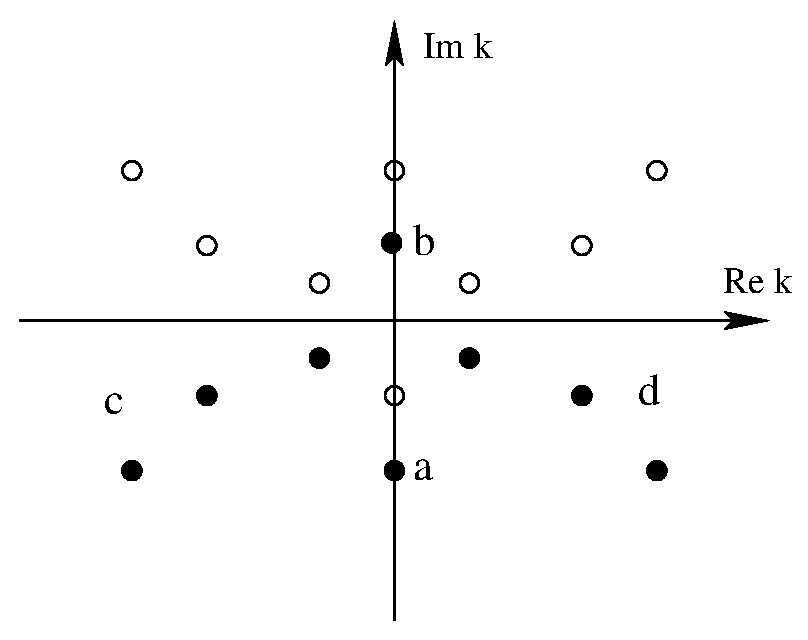
\epsfig{file=figures/smat_poles.eps}}
\end{center}
\caption{Distribution of $S-$ matrix poles (filled circles) and corresponding
  zeroes (open circles) in the complex $k-$plane. $a =$ anti-bound, 
 $ b = $ bound, $c = $ capture and $d =$ decay.}  
\label{fig:smat_poles}
\end{figure}

\section{Regularizing divergent integrals of states on the second energy sheet.}
\label{sec:divergent_integrals}
The radial wave function $u_l(k,r)$ of a decay 
resonant state, with $k = k_n$ located in the fourth quadrant of the complex
$k-$plane, satisfies the radial Schr\"odinger equation ~(\ref{eq:chap21_eq1}).
The decay resonances are regular at the origin, $ u_l(k,0) = 0$, 
and have purely outgoing waves, $u_l(k,r) \rightarrow O_l(k,r)$, at infinity 
as  boundary conditions. 
If the potential has a finite range, in the sense
that it vanishes identically beyond some finite distance $r=a$. The outgoing
solutions $O_l(kr)$ 
are given in terms of spherical Riccati-Hankel functions $h_l^{(+)}(kr)$.
In the case of long-range potentials, such as the Coulomb potential, 
the asymptotic form of the wave functions are given by the  more complicated
Coulomb functions.

From the requirement that the wave functions and their derivatives should be
continuous at the boundary of the potential $r=a$, follows that the logarithmic 
derivative should be continuous, giving the condition
\begin{equation}
  u_l(k,a){O'}_l(k,a) - {u'}_l(k,a)O_l(k,a) = 0.
\end{equation}
For each pole $k=k_n$ in the fourth 
quadrant there is a pole $k=\tilde{k}_n=-k_n^*$ in the third quadrant 
associated with a capture resonance. The capture
states, $ u_l(\tilde{k}_n,r)$, 
are solutions of the complex conjugated version of 
the radial Schr\"odinger equation (\ref{eq:chap21_eq1}), with  regularity at the 
origin and with purely incoming waves at infinity, $I_l(k,r)$. 
Where $I_l(kr)$ 
is given in terms of spherical Riccati-Hankel functions $h_l^{(-)}(kr)$.
The corresponding boundary conditions for the capture states becomes, 
\begin{equation}
  {u}_l(\tilde{k},a){I'}_l(\tilde{k},a) - {{u}'}_l(\tilde{k},a)I_l(\tilde{k},a) = 0.
\end{equation}
In the following we define the the decay and capture states by
\begin{equation} 
  u_{nl}(r) \equiv u_l(k_n,r), \:\: \tilde{u}_{nl}(r) \equiv u_l(\tilde{k}_n,r) 
\end{equation}
The capture and decay resonances are related through 
\begin{equation} 
  \tilde{u}_{nl}(r) = u_{nl}^*(r), \:\: \mathrm{i.e.} \:\: \tilde{u}_{nl}^*(r) = u_l(r)
\end{equation}
Normalization of the decay resonances through the usual Euclidean inner product, 
\begin{equation}
  \langle {u}_{nl} \vert u_{nl}\rangle=
  \int_0^\infty dr\: u_{nl}^*(r)u_{nl}(r) = 
  \int_0^\infty \tilde{u}_{nl}(r)u_{nl}(r) 
\end{equation}
is not possible in the upper limit, since the integrand diverges exponentially as 
\begin{equation}
  \tilde{u}_{nl}(r)u_{nl}(r) \mathop{\longrightarrow}_{r\rightarrow\infty} 
  e^{2 k_2 r}
\end{equation}
for $k_n = k_1 -ik_2 $ and $k_1,k_2 > 0 $.
On the other hand, the fact the decay and capture resonances come in conjugate pairs,
may suggest that they form a \emph{bi-orthogonal} set 
of functions, and that the normalization integral,
\begin{equation}
  \langle \tilde{u}_{nl} \vert u_{nl}\rangle = \int_0^\infty \tilde{u}_{nl}^*(r)u_{nl}(r) = 
  \int_0^\infty u_{nl}^2(r), 
\end{equation}
may exist, and be given a definite value.
The integrand of this integral still increases exponentially but 
oscillates as 
\begin{equation}
  \tilde{u}_{nl}^*(r)u_{nl}(r) \mathop{\longrightarrow}_{r\rightarrow\infty} 
  e^{ 2ir \left( k_1 -ik_2\right) }.
  \label{eq:eq220}
  %\label{eq:eq220}
\end{equation}
The hope is that the oscillations at large distances will cancel each other, 
such that 
\begin{equation}
  0 < \vert \langle \tilde{u}_l(k) \vert u_l(k)\rangle \vert < \infty
\end{equation}

\subsection{Regularization by $e^{-\epsilon r^2}$.}

From the theory of divergent integrals and series, see e.g. Ref.~\cite{hardy}, 
many integrals which are divergent in the conventional sense, may be regularized by some
regularization procedure. Zel'dovich \cite{zeldovich} proposed the following 
integration procedure for regularizing integrals involving resonant states,
which have an exponentially oscillating divergent tail along the real $r$-axis. 
\begin{equation}
  I = \mathop{\lim}_{\epsilon \rightarrow 0}\int_0^\infty dr\:e^{-\epsilon r^2}u_{nl}^2(r)
  \label{eq:norm_int}
\end{equation}
From the asymptotic behaviour of the resonant states in equation~(\ref{eq:eq220}), it 
is natural to study the integral 
\begin{equation}
  I_n(k) = \mathop{\lim}_{\epsilon \rightarrow 0} I_n(k,\epsilon) = 
  \mathop{\lim}_{\epsilon \rightarrow 0}\int_0^\infty dr\:e^{-\epsilon r^2}r^n e^{\kappa r} ,
\end{equation}
where $n = 0,1 $ and $ \kappa = i k$. For a positive and finite value $\epsilon$ 
the regularizing factor $e^{-\epsilon r^2}$ decreases more rapidly than the 
exponential function  $ e^{\kappa r}$ increases for an arbitrary exponent $\kappa$, and 
the integral �$I_n(k,\epsilon)$ converges. It is convienient to introduce a variable
change in $I_0(k,\epsilon)$
\begin{equation}
  t = r\sqrt{\epsilon}, \:\: x = {\kappa \over 2 \sqrt{\epsilon}} 
\end{equation}
which gives
\begin{equation}
  I_0(k,\epsilon) = {1\over \sqrt{\epsilon}}e^{x^2}\int_{-x}^\infty dt\: e^{-t^2} = 
  \sqrt{ { \pi\over \epsilon}}e^{x^2}\left[ 1 - 2\mathrm{Erfc}(x)\right]
\end{equation}
where 
\begin{equation}
  \mathrm{Erfc}(x) = {2\over \sqrt{\pi}}\int_x^\infty dt\: e^{-t^2}.
\end{equation}
is the complementary error function \cite{boas}. As $\epsilon \rightarrow 0 $ 
then $ x \rightarrow \infty $, and using the asymptotic expansion of the error function \cite{boas}, the
integral $I_0(k,\epsilon) $ may be written as 
\begin{eqnarray}
  \nonumber
  I_0(k,\epsilon) & = & \sqrt{\pi \over \epsilon}e^{x^2} - 
  {1\over 2x\sqrt{\epsilon}}\left( 1 - {1\over 2x^2} + {3\over 4x^4} - ...\right)  \\  
  & = & \sqrt{\pi \over \epsilon}e^{-{k^2\over 4\epsilon}} + {i\over k} -{2\epsilon \over k^3} + O(\epsilon^2).
  \label{eq:eq227}
  %\label{eq:asymp2}
\end{eqnarray} 
The integral $I_1(k,\epsilon)$ is calculated using the relation,
\begin{equation}
  I_1(k,\epsilon) = {\partial \over \partial \kappa} I_0(k,\epsilon) = 
  {1\over 2\epsilon}\left( \kappa I_0(k,\epsilon) +1 \right),  
\end{equation} 
Inserting the asymptotic expansion for $I_0(k,\epsilon)$ in equation~(\ref{eq:eq227}), 
gives for the $I_1(k,\epsilon)$ integral,
\begin{equation}
  I_1(k,\epsilon) = -\sqrt{ \pi \over 4\epsilon^3 }ike^{-{k^2\over 4\epsilon} } - {1\over k^2} + O(\epsilon).
\end{equation}  
Dealing with regularization of integrals involving \emph{proper} resonances, 
in which the real part of the resonance energy is positive,
the restriction  $\vert \mathrm{Re}\:k\vert > \vert \mathrm{Im}\:k \vert $ follows, and 
consequently $ \mathrm{Re}\:k^2 > 0$.�In this case the relation 
\begin{equation}
  \mathop{\lim}_{\epsilon \rightarrow 0} \epsilon^p e^{ -{k^2 \over 4\epsilon} } = 0,
 \end{equation}
is valid for any real $p$, and may be used to obtain the following 
finite expressions for the integrals $I_0(k)$ and $I_1(k)$,
\begin{equation}
  I_0(k) = { i\over k}, \:\: I_1(k) = -{1 \over k^2}.
\end{equation}

\subsection{Regularization by complex scaling.}
The regularization factor $e^{-\epsilon r^2}�$ is not unique, and there exists 
a variety of other regularization procedures,  all yielding the same unique finite
result for the integrals $I_1(k)$ and $I_2(k)$. One such regularization procedure,
more tractable from a numerical standpoint, is based on complex rotation in the complex
$r$-plane, first discussed in Ref.~\cite{gyarmati}.
Consider the zero contour integrals 
\begin{equation}
  \int_C dz\: e^{ik z} = 0, \:\:  \int_C dz\: z e^{ik z} = 0,
 \end{equation}
where the contour $C=C_1 + C_2 + C_3 $ is defined by a rotation angle $\theta$ 
in the complex $r$-plane as shown in figure~\ref{fig:rcontour}.  
\begin{figure}[hbtp]
\begin{center}
\resizebox{10cm}{8cm}{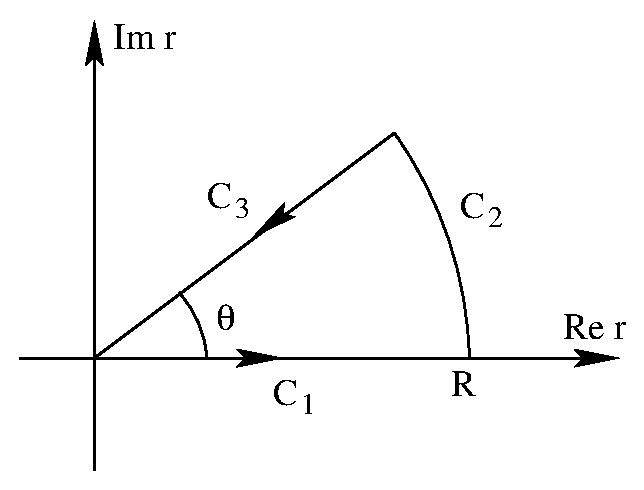
\epsfig{file=figures/rcontour.eps}}
\end{center}
\caption{Integration contour in the complex�$r$-plane used for
  regularization of integrals involving resonant states.}
\label{fig:rcontour}
\end{figure}
For $R\rightarrow \infty $ the integral along the arc $C_2$ vanishes and 
by the Cauchy Riemann integral theorem it follows 
\begin{eqnarray}
  \tilde{I}_0(k) = \int_0^\infty dr\: e^{ik r} 
  = e^{i\theta} \int_0^\infty  dr\: e^{ik r \left( \cos\theta + i\sin\theta\right)} \\
  \tilde{I}_1(k) = \int_0^\infty dr\: r e^{ik r} 
  = e^{2 i\theta} \int_0^\infty  dr\: r e^{ik r \left( \cos\theta + i\sin\theta\right)}. \\
\end{eqnarray}
For $k = k_1 - ik_2$ and $k_1,k_2 > 0$ these integrals converge for a rotation angle 
$ \theta > \mathrm{atan}( k_2/k_1) $, and it is easily shown that they take the finite
values
\begin{equation}
  \tilde{I}_0(k) = {I}_0(k) = {i\over k},
\end{equation}
In the same way it is easily shown that 
the integral $\tilde{I}_2(k)$ takes the finite value
\begin{equation}
  \tilde{I}_1(k) = {I}_1(k) = -{1\over k^2},
\end{equation}
illustrating that different regularization procedures of divergent integrals 
must yield the same unique finite value, if it exists.

From the above 
analysis it is found that the innerproduct given in equation~(\ref{eq:norm_int})
of a $d$ - and the corresponding conjugate $c$ resonant state 
may be given a finite value, i.e. it is possible to normalize these states.
It remains to examine whether resonant states at different energies, i.e. 
$k_1 \neq k_2$, form a \emph{bi-orthogonal} set. Starting with the Schr\"odinger equation 
for two different resonant states $u_{n_1l}(r)$ and $ u_{n_2l}(r)$ and multiplying the 
left with $u_{n_2l}(r)$ and $ u_{n_1l}(r)$ respectively, one obtains by subtracting the 
two equations,
\begin{equation}
  {d\over dr}\left[ u_{n_2l}(r)u'_{n_1l}(r) - u'_{n_2l}(r)u_{n_1l}(r)\right] = 
  \left( k_2^2 -k_1^2 \right) \tilde{u}_{n_2l}^*(r)u_{n_1l}(r).
 \end{equation}
Multipying from the left with $\int_0^\infty dr\: e^{-\epsilon r^2}$, 
one obtains the following expression by partial integration,
\begin{eqnarray}
  \nonumber
  \int_0^\infty dr\: e^{-\epsilon r^2} {d\over dr}\left[ u_{n_2l}(r)u'_{n_1l}(r) - u'_{n_2l}(r)u_{n_1l}(r)\right]  = \\
  \nonumber
  2\epsilon \int_0^\infty dr\: r e^{-\epsilon r^2}\left[ u_{n_2l}(r)u'_{n_1l}(r) - u'_{n_2l}(r)u_{n_1l}(r)\right]  \\
  = \left( k_2^2 - k_1^2 \right)\int_0^\infty dr\: e^{-\epsilon r^2}\tilde{u}_{n_2l}^*(r)u_{n_1l}(r), 
  \label{eq:eq239}
  %\label{eq:norm_int2}
\end{eqnarray}
where the boundary condition $u_{nl}(r=0) = 0$ has been used. 
From the asymptotic form of the integrand 
$ r e^{-\epsilon r^2}�e^{i(k_1 + k_2)r} $  it is seen that the integrals in equation~(\ref{eq:eq239})
are comparable with the finite result for the integral $I_1(k,\epsilon)$
as $\epsilon \rightarrow 0$. It follows that 
\begin{equation}
  \left( k_2^2 - k_1^2 \right)\mathop{\lim}_{\epsilon \rightarrow 0} 
  \int_0^\infty dr\: e^{-\epsilon r^2}\tilde{u}_{n_2l}^*(r)u_{n_1l}(r) = 0. 
\end{equation}
Defining the inner product of resonant states as this limit, we finally obtain 
\begin{equation}
  \langle \tilde{u}_{n_1l} \vert u_{n_2l} \rangle = 
  \langle {u}_{n_1l}^* \vert u_{n_2l} \rangle = \delta_{n_1,n_2},
  \label{eq:eq241}
  %\label{eq:cproduct}
\end{equation}
which shows that the resonant states together with the bound states
are orthogonal in this sense. In the case where bound states enter the 
inner product, there is no divergence problem since the bound states 
has an exponential decay as $r\rightarrow \infty$.
This symmetric inner product is often called the $c$- product \cite{nimrod}, 
which states that the resonances form a \emph{bi-orthogonal} set. In the case where 
$k_1$ and $k_2$ are real, the $c$-product coincides with the usual Hermitian inner product.

 
\section{The generalized Berggren completeness; proof and discussion}
\label{sec:berggren}
We have shown that the regular solution $\phi_l(k,r)$ with 
$k=k_n$ being the poles of the scattering matrix or zeros of the Jost function, can 
be normalized by some regularization procedure. Further it was shown that
regular solutions $\phi_l(k,r)$ located at different $k_n$ 
in the complex $k$-plane are orthogonal to each other, 
through the symmetric inner product given in equation~(\ref{eq:eq241}). This 
suggests that the regular solutions at the 
poles of the scattering matrix, are part of a complete set of 
\emph{bi-orthogonal}�states, which may serve as an expansion basis 
when dealing with processes taking place in the continuum regime. This is the
subject of this section. 

We start with the standard completeness relation 
defined along the real $k$-axis, 
\begin{equation}
  \sum_{n=b} u_{ln}(r)u_{nl}^*(r')\vert + 
      {1\over 2}�\int_{-\infty}^\infty dk\: u_l(k,r) u_l^*(k^*,r') = \delta(r-r')
      \label{eq:eq242}
\end{equation}
where the discrete sum is over the bound state poles located along the 
positive imaginary $k$-axis, and the integral is over the continuum of 
scattering functions located along the real $k$-axis. Note that on the real axis 
we have $u_l^*(k^*,r') = u_l^*(k,r') $.
A proof of this completeness is given by Newton in Ref.~\cite{newton}. Newton considered 
the integral 
\begin{equation}
  I(r) = \int_C dk\:k\int_0^\infty d{r'}\: h(r')G_l(k;r,r'),
  \label{eq:eq243}
  %kanskje litt mere utfyllende om Newtons bevis...
\end{equation}
where $h(r)$ is part of the L$^2$ functional space and $G_l(k;r,r')$ is 
the complete Green's function or resolvent. The integration contour 
$C$�
runs along the real $k$-axis from $-\infty $ to $\infty $, and is closed 
by a semicircle in the upper half $k$-plane. The Green's function has 
poles at the same locations in the complex $k$-plane as the 
scattering matrix, and using Cauchy's residue theorem the various contributions 
to the integral in equation~(\ref{eq:eq243}) is evaluated by the residues at the
bound state poles along the positive imaginary $k$-axis. In the end it is 
shown that a $l^2$ function $h(r)$ may be expanded in a complete
set of bound- and scattering wave functions given in equation(\ref{eq:eq242}).
The class of square integrable functions, includes those with 
exponential asymptotics, $ h(r) \rightarrow e^{ikr}, \: r \rightarrow \infty $, 
where $k$ is in the upper half complex $k$-plane.  

\begin{figure}[hbtp]
\begin{center}
\resizebox{12cm}{9cm}{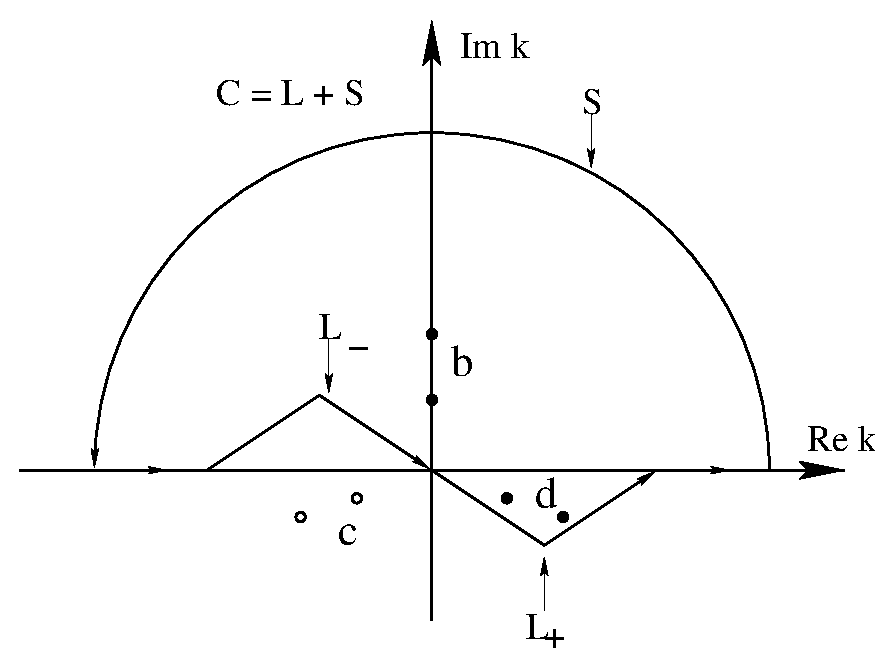
\epsfig{file=figures/int_contour1.eps}}
\end{center}
\caption{Integration contour $C = L +S$ used in deriving the Berggren completeness relation.}
\label{fig:int_contour1}
\end{figure}
In Ref.~\cite{berggren} Berggren showed that there exist 
a modified completeness relation, where the resonant contributions hidden in the
continuum integral were disentangled from the background of continuum states, 
and included in the discrete sum over bound states.
The proof of Berggren, is based on the same complex analysis used by Newton,  
only that the integration contour $C$ in equation~(\ref{eq:eq243}) where modified to enclose not
only the bound state poles, but in addition a set of \emph{proper}�
resonant poles, 
see figure~\ref{fig:int_contour1}.

Later Lind \cite{lind} presented a straightforward method for deriving 
various completeness relations starting from the standard 
completeness relation given in equation~(\ref{eq:eq242}). 
This method is based on analytic 
continuation of the integral over scattering functions, using the 
the known analytic properties of the scattering functions in the complex
$k$-plane. As discussed in the previous section \ref{sec:physical_interpretation}, the
scattering functions have poles wherever the Green's function $G_l(k)$ or the scattering matrix 
elements $S_l(k)$ have poles. Deforming the integration contour defined
along the real $k$-axis for the continuum integral in equation~(\ref{eq:eq242}), one obtains 
by the Cauchy residue theorem
\begin{equation}
  �-\int_{0}^\infty dk\: u_l(k,r) \tilde{u}_l^*(k,r') + 
   \int_{L^+} dk\: u_l(k,r) \tilde{u}^*_l(k,r') = 
   2\pi i \sum_{k_n \in  {\bf C}} \mathop{\mathrm{Res}}_{k = k_n} u_l(k,r) \tilde{u}^*_l(k,r'),
   %\label{eq:int_contour2}
   \label{eq:eq244}
\end{equation}
where the contour $L^+$ is part of the inversion symmetric contour $L = L^- +L^+$, and is
the deformation of the positive real $k$-axis. Here $\tilde{u}_l(k,r) = u_l(k^*,r)$ are associated 
with scattering functions on the conjugated contour $L^*$,  which  encloses the capture 
resonances which are orthogonal to the decay resonances enclosed by $L$. 
Inversion symmetric contour meaning that if $k$ is on $L$, then so is $-k$. 
The product of scattering functions $ u_l(k,r) \tilde{u}_l(k,r') $ is a meromorphic function of
$k$ with poles given by the Jost functions $f_l(-k) = 0 $ and  $f_l^*(-k^*) =0 $.
The residue is evaluated 
at each pole $k=k_n$ of the scattering functions, 
located in the region between the contour $L^+$ and 
the real positive $k$-axis labeled ${\bf C}$.
In writing equation~(\ref{eq:eq244}) the inversion symmetry of $L$ and the 
symmetry of the integrand in the continuum integral has been exploited to give
\begin{equation}
  \int_{L^-} dk\: u_l(k,r)  \tilde{u}_l^*(k,r') = 
  \int_{L^+} dk\: u_l(k,r)  \tilde{u}_l^*(k,r')
\end{equation}
In Ref.~\cite{lind} the importance of choosing an inversion symmetric contour was discussed. If $L$ is 
inversion symmetric, the complex continuum integral can be rewritten in terms of scattering functions,
and the continuum integrals can be written using energy as the integration variable.
In deriving the general Berggren completeness the residues in equation~(\ref{eq:eq244}) 
have to be evaluated. Writing the physical wave function in terms of the 
regular solution and the Jost  function, see Sec.~\ref{sec:physical_interpretation}
for further details, one gets
\begin{equation}
  u_l(k,r) = \sqrt{2\over \pi} {k^{l+1}\phi_l(k,r)\over f_l(-k)},
\end{equation}
and for the conjugate wave function $\tilde{u}_l(k,r)$,
\begin{equation}
  \tilde{u}_l(k,r) = u_l(k^*,r) = \sqrt{2\over \pi} {(k^*)^{l+1}\phi_l(k^*,r)\over f_l(-k^*)} = 
  \left(  \sqrt{2\over \pi} {k^{l+1}\phi_l(k,r)\over f_l(k)} \right)^*,
\end{equation}
where use has been made of the symmetry properties of the regular and Jost functions
given in equation~(\ref{eq:symmetry}). The residue in equation~(\ref{eq:eq244}) may then 
be written as
\begin{equation}
  \mathop{\mathrm{Res}}_{k = k_n} u_l(k,r) \tilde{u}_l^*(k,r') = 
  \mathop{\mathrm{Res}}_{k = k_n} {2\over \pi} {k^{2l+2}\phi_l(k,r)\phi_l(k,r')\over f_l(k)f_l(-k)},
  \label{eq:residue}
\end{equation}
Making use of the property $\mathop{\mathrm{Res}}_{z = z_0} h(z)/g(z) = h(z_0)/g'(z_0) $ 
where $h(z)$ and $g(z)$ are analytic functions at $z=z_0$, it is seen that following 
derivative has to be evaluated, 
\begin{equation}
\left. {d\over dk} f_l(k)f_l(-k) \right| _{k=k_n} = 
 f_l(k_n) \left. {d\over dk}f_l(-k)\right| _{k=k_n},
\end{equation}
here the fact the Jost function $f_l(-k) = 0 $ for $k=k_n$  has been used. 
The problem of determining the residue in equation~(\ref{eq:eq244}) has now been reduced to 
the problem of determining the derivative of the Jost function at the resonance pole $k=k_n$.
In Ref.~\cite{lind} the derivative of the Jost function where proven to be 
\begin{equation}
 \left. {d\over dk}f_l(-k)\right| _{k=k_n} = i4k_n^{2l+2} Reg \int_0^{\infty} dr r^2\phi^2_l(k_n,r) = 
 i4k_n^{2l+2}N^2,
\end{equation}
where $N$ is the norm of the regularized resonances wave functions appearing in the integral. 
The sum over residues in equation~(\ref{eq:eq244}) now becomes, 
\begin{eqnarray}
\nonumber
  2\pi i \sum_{k_n \in {\bf C}} \mathop{\mathrm{Res}}_{k = k_n} u_l(k,r) \tilde{u}^*_l(k,r') = 
  4i \sum_{k_n \in {\bf C}}  {k^{2l+2}\phi_l(k_n,r)\phi_l(k_n,r')\over 
    \left. {d\over dk} f_l(k)f_l(-k)\right|_{k=k_n}} \\ 
  = \sum_{k_n \in {\bf C}} {\phi_l(k_n,r)\phi_l(k_n,r')\over N^2} = \sum_{k_n \in {\bf C}} u_{nl}(r)\tilde{u}_{nl}^*(r'),
\end{eqnarray}
inserting this into equation~(\ref{eq:eq244}), one gets the following expression for 
the integral over scattering functions along the real $k$-axis (positive energy states),  
\begin{equation}
  �\int_{0}^\infty dk\: u_l(k,r)  \tilde{u}_l^*(k,r') = 
   \sum_{k_n \in  {\bf C}} u_{nl}(r) \tilde{u}_{nl}^*(r') + 
   \int_{L^+} dk\: u_l(k,r)  \tilde{u}_l^*(k,r'),
\end{equation}
where it is explicitly seen that the resonant contributions hidden in the the continuum 
integral along the real $k$-axis has been disentangled. In Ref.~\cite{lind} it was shown 
for finite range potentials that the continuum integral along the contour $L^+$ produces
a smooth background, but is in most cases non-neglible. Switching to abstract vector notation,
it has been shown that for a general inversion symmetric 
contour $L$, see figure~\ref{fig:int_contour2}, the generalized Berggren 
completeness becomes, 
\begin{equation}
  {\bf 1} = \sum_{n= a,b,c,d} \vert u_{nl}\rangle \langle \tilde{u}_{nl}\vert + 
  �\int_{L^+} dk\:\vert u_l(k) \rangle \langle \tilde{u}_l(k)\vert.  
   %\label{eq:berggren}
   \label{eq:eq248}
\end{equation}
The discrete sum includes all types of poles of the scattering matrix, i.e.
anti-bound (a), bound (b), capture resonant (c) and decay resonant (d) states. This 
completeness can be used to expand all functions with exponential asymptotics,  
$e^{ikr}, \: r \rightarrow \infty �$ where $k$ is located within the closed
contour $C= L+S$. Keeping only the discrete part of the completeness 
relation (\ref{eq:eq248}), one ends up with the pole-approximation.   
\begin{figure}[hbtp]
\begin{center}
\resizebox{12cm}{9cm}{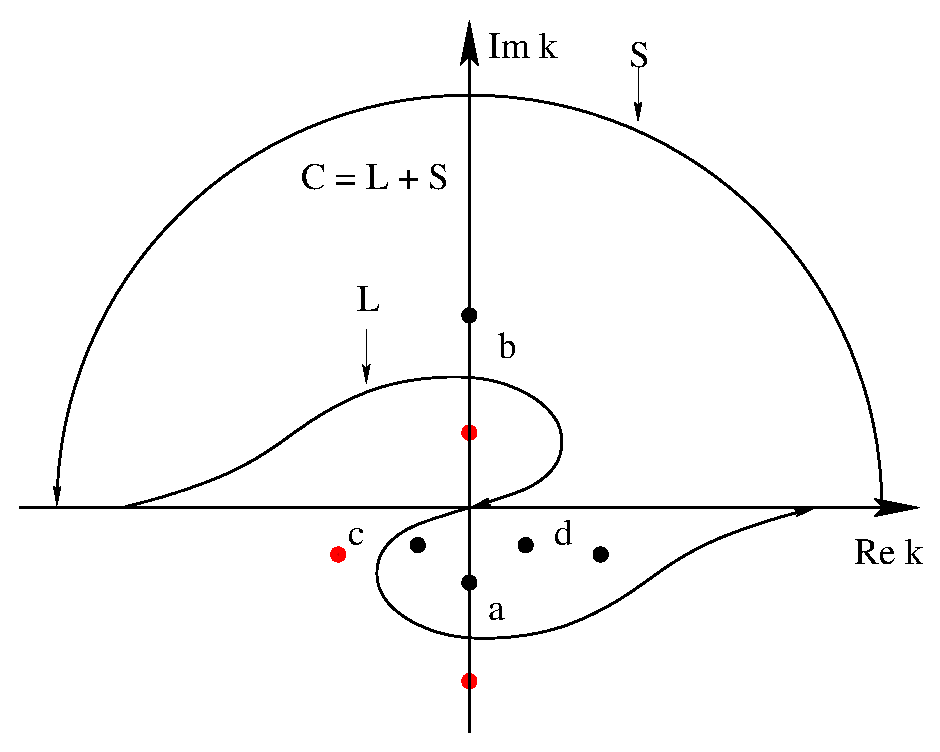
\epsfig{file=figures/int_contour2.eps}}
\end{center}
\caption{General inversion symmetric contour $C = L +S$ used in deriving the 
  generalized Berggren completeness relation. The black circles represents the poles which 
  are included in the discrete sum, while the red circles are poles which are embedded in the 
  continuum integral along the contour $L^+$.} 
\label{fig:int_contour2}
\end{figure}
As shown in figure~\ref{fig:int_contour2} a typical inversion symmetric 
contour cannot separate all poles from the continuum integral. In this particular case
the red circles gives the poles which are not included in the discrete sum, while
the black circles give the poles which are included in the sum. It is important to emphasize 
that completeness defined either along the real $k$-axis or along a distorted contour $L$ in 
the complex $k$-plane are equivalent in the sense, 
\begin{eqnarray}
  \nonumber
      {\bf 1} & = & \sum_{n= a,b,c,d} \vert u_{nl}\rangle \langle \tilde{u}_{nl}\vert + 
      �\int_{L^+} dk\:\vert u_l(k) \rangle \langle \tilde{u}_l(k)\vert \\
       & = &  \sum_{n= b} \vert u_{nl}\rangle \langle \tilde{u}_{nl}\vert + 
       �\int_{0}^\infty dk\:\vert u_l(k) \rangle \langle \tilde{u}_l(k)\vert 
	\label{eq:eq249}
	%\label{eq:eq249}
\end{eqnarray} 
the difference being that for a completeness defined along the real $k$-axis
all the interesting processes taking place in the continuum are hidden as peaks within the 
continuum integral, while for a completeness defined along $L$ the most 
interesting phenomena, i.e. the resonant contributions,  
are extracted out of the continuum integral and can be studied separately.



\section{Interpretation of complex observables}
\label{sec:observables}
Turning to the interpretation of expectation values of observable operators 
involving resonant states, it is natural to ask what physical meaning
one should assign to such expectation values. The resonant states are complex, yielding 
complex expectation values of the Hamiltonian $H$ and any other Hermitian observable operator $A$.  
If resonant states are to be seen as excited states in which a particular system can 
undergo transition from and to, and such transitions are expected to be seen experimentally, 
a physical interpretation of the real and imaginary parts of $\langle A \rangle $ is 
necessary. This question was first raised by Berggren \cite{berggren} and later by 
Gyarmati et. al. \cite{gyarmati2}, where it was 
conjectured that the physical meaning of an expectation value $\langle A \rangle $ 
when the system is in a resonant state is given by the real part, 
\begin{equation}
  \langle A \rangle  = \mathrm{Re}�\langle \tilde{u}_{nl}\vert A \vert {u}_{nl}\rangle
  \label{eq:eq250}
\end{equation}
A theoretical justification of this conjecture was 
given by Berggren in Ref.~\cite{berggren2}, where it 
was shown starting from scattering theory, 
that the real part of the complex cross section for populating 
a resonance is equal to the energy integral of the in-elastic continuum 
cross section across the resonance peak. The imaginary part of the cross section 
where identified with the strength of the resonance-background interference.
In Ref.~\cite{berggren3} this conclusion where generalized to hold for any observable operator $A$ 
involving resonant states. To throw some light on this interpretation,
consider the matrix element of an operator $A$ with 
a scattering function defined on the real energy axis, 
\begin{equation}
  \langle \tilde{u}_l(k) \vert A \vert u_l(k) \rangle �= \mathrm{Re}\langle \tilde{u}_l(k) \vert A \vert u_l(k) \rangle. �
  \label{eq:eq251}
\end{equation}
Suppose now that the Jost function $f_l(-k)$  has a zero located close to
the real $k$-axis, which is associated with a narrow resonance. Since the scattering
wave functions have poles wherever the Jost functions have zeroes, see equation~(\ref{eq:chap21_eq8}) of section 
\ref{sec:physical_interpretation},  
the matrix element \ref{eq:eq251} will display a sharp peak 
when it is plotted as a function of energy, and the energy traverses the 
real part of the resonance energy. The momentum (energy)-integrated matrix elemenent 
is,
\begin{eqnarray}
  \nonumber
  \int_0^{k_\mathrm{max}} dk\: \langle \tilde{u}_l(k) \vert A \vert u_l(k) \rangle = \\ 
  \int_C dk\: \langle \tilde{u}_l(k) \vert A \vert u_l(k) \rangle 
  -2\pi i \mathop{\mathrm{Res}}_{k = k_n}  \langle \tilde{u}_l(k) \vert A \vert u_l(k) \rangle,
  \label{eq:energy_int}
\end{eqnarray}
where $C$ is a contour in the fourth quadrant of the complex $k$-plane enclosing the pole 
at $k=k_n$, and joining the real axis at�$k=0$ and $k= k_{\mathrm{max}}$, see figure~\ref{fig:int_contour3}. 
\begin{figure}[hbtp]
\begin{center}
\resizebox{10cm}{6cm}{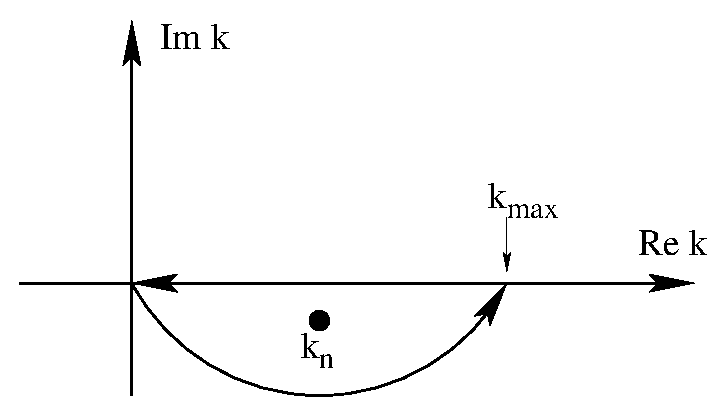
\epsfig{file=figures/int_contour3.eps}}
\end{center}
\caption{Integration contour used in evaluating the pure resonance contribution to the 
  energy-integrated expectation value.}
\label{fig:int_contour3}
\end{figure}
The residue in equation~(\ref{eq:energy_int}) is given by equation~(\ref{eq:residue}) from the previous section, and
consequently,  
\begin{eqnarray}
  \nonumber
  \int_0^{k_\mathrm{max}} dk\: \langle \tilde{u}_l(k,r) \vert A \vert u_l(k,r) \rangle = \\ 
  \nonumber
  \int_C dk\: \langle \tilde{u}_l(k,r) \vert A \vert u_l(k,r) \rangle 
  + \langle \tilde{u}_{nl} \vert A \vert u_{nl} \rangle = \\
  \mathrm{Re}\int_C dk\: \langle \tilde{u}_l(k) \vert A \vert u_l(k) \rangle 
  + \mathrm{Re}\langle \tilde{u}_{nl} \vert A \vert u_{nl} \rangle.
\end{eqnarray}
Since the expectation value is by definition real, the imaginary parts of the 
contour integral of the scattering functions and the imaginary part of the 
matrix element involving the resonance at $k=k_n$ must cancel, in this 
way it is illustrated that the imaginary part of 
$\langle \tilde{u}_{nl} \vert A \vert u_{nl} \rangle $ may be interpreted as 
an interference effect with the continuum background.

Assuming now that equation~(\ref{eq:eq250}) is a reasonable physical interpretation 
of the formal expectation value $ \langle \tilde{u}_{nl}\vert A \vert u_{nl}\rangle $,
what meaning should one assign the imaginary part? 
Let us start with the usual definition of the average deviation, or indeterminacy, 
of an operator $A$ which is assumed to commute with the Hamiltonian $H$, 
\begin{equation}
  \left( \Delta A\right)^2 = \langle A^2 - \langle A \rangle^2 \rangle = 
  \langle A^2 \rangle - \langle A \rangle^2 
  %\label{eq:deviation}
  \label{eq:eq254}
\end{equation}
Using the definition of $\langle A \rangle $ in equation~(\ref{eq:eq250}), it 
is easily found that 
\begin{equation}
  \langle A^2 \rangle = \mathrm{Re}\langle \tilde{u}_{nl} \vert A^2 \vert u_{nl}\rangle = 
  \left[ \mathrm{Re}\langle \tilde{u}_{nl} \vert A \vert u_{nl} \rangle \right]^2 - 
  \left[ \mathrm{Im}\langle \tilde{u}_{nl} \vert A \vert u_{nl} \rangle \right]^2
\end{equation}
and 
\begin{equation} 
  \langle A \rangle^2  =  \left[ \mathrm{Re}\langle \tilde{u}_{nl}\vert A \vert u_{nl}\rangle \right]^2. 
\end{equation}
Inserting this into equation~(\ref{eq:eq254}) yields,
\begin{equation}
  \left( \Delta A\right)^2 = \langle A^2 - \langle A \rangle^2 \rangle =  
  -\left[ \mathrm{Im}\langle \tilde{u}_{nl} \vert A \vert u_{nl}\rangle \right]^2.
  \label{eq:eq257}
\end{equation}
Thus is is then formally shown that the imaginary part of the expectation value of 
an operator $A$ in a resonant state, gives the uncertainty or indetermiacy of 
the measured result. This may also be understood from physical grounds. 
Resonant states have definite lifetimes, i.e. they decay in time. The
lifetime of the resonant state is determined by the propability of tunneling 
through the potential barrier, in which the resonance is formed. The probability 
of decay is proportional to the imaginary part of the resonance pole or in other 
words the resonance width $\Gamma $. Let the operator $A$ be the Hamiltonian of 
the system, $A = H$, then equation~(\ref{eq:eq257})�becomes, 
\begin{equation}
  \left( \Delta H\right)^2 = \langle H^2 - \langle H \rangle^2 \rangle = -{\Gamma^2 \over 4}, � 
\end{equation}
where it is explicitly seen that by the defintion of $\langle H \rangle $,�
the width $\Gamma $ determines the uncertainty in energy measurements. 
%
%  some words on my approach and how the thesis is composed....
%



\chapter{Contour deformation method (CDM) in momentum space; theory and applications}
\section{The momentum space Schr\"odinger equation.}
\label{sec:momspace}
The Schr\"odinger equation in abstract vector representation is
\begin{equation}
  \left( T + V \right) \vert \psi_n \rangle = E_n \vert\psi_n \rangle 
  \label{eq:vec_rep}
\end{equation}
Here $T$ is the kinetic energy operator and $V$ is the potential operator. 
The eigenstates form a complete orthonormal set according to 
\[ 
{\bf 1} = \sum_n \vert \psi_n\rangle\langle \psi_n \vert, \:\: \langle \psi_n\vert \psi_{n'} \rangle = \delta_{n,n'}
\]
The most commonly used representations of equation~\ref{eq:vec_rep} are the coordinate
and
the momentum space representations. They define the completeness relations 
\begin{eqnarray}
 {\bf 1}&  = &  \int d{\bf r} \:\vert  {\bf r} \rangle \langle {\bf r}\vert, \:\: 
 \langle  {\bf r}\vert  {\bf r'} \rangle = \delta ( {\bf r}-{\bf r'}) \\
{\bf 1} & = & \int d{\bf k} \:\vert  {\bf k} \rangle \langle {\bf k}\vert, \:\: 
  \langle  {\bf k}\vert  {\bf k'} \rangle = \delta ( {\bf k}-{\bf k'}) 
\end{eqnarray}
Here the basis states in  both ${\bf r}$- and ${\bf k}$-space are dirac-delta 
function normalized. From this it follows that the plane-wave states are given by,
\footnote{Some authors define the plane wave by  $ \langle  {\bf r}\vert  {\bf k} \rangle = 
  \exp \left( i {\bf k\cdot r} \right) $, in which case 
  $ \langle  {\bf k}\vert  {\bf k'} \rangle = \left( 2\pi \right)^3 \delta ( {\bf k}-{\bf k'}) $
  and each $\int d{\bf k}$ is replaced by $ (1/2\pi)^{3/2}\int d{\bf k} $.}�
\begin{equation}
  \langle  {\bf r}\vert  {\bf k} \rangle = \left( 1\over2\pi \right)^{3/2}\exp \left( i {\bf k\cdot r} \right)
  \label{eq:planewave1}
\end{equation}
which is a transformation function defining the mapping from the abstract 
$ \vert {\bf k} \rangle $ to the abstract $\vert {\bf r}\rangle $ space.
That the ${\bf r}$-space basis states are 
delta-function normalized follows from 
\begin{equation}
  \delta ( {\bf r}-{\bf r'}) = \langle {\bf r} \vert {\bf r}'\rangle = 
  \langle {\bf r} \vert {\bf 1} \vert {\bf r}'\rangle = 
  \int \mathrm{d}{\bf k}�\langle {\bf r}\vert {\bf k} \rangle \langle {\bf k}\vert {\bf r}' \rangle = 
  \left( {1\over 2\pi}\right)^3 \int \mathrm{d}{\bf k} e^{i {\bf k}({\bf r} - {\bf r}')} 
\end{equation}
and the same for the momentum space basis states,
\begin{equation}
  \delta ( {\bf k}-{\bf k'}) = \langle {\bf k} \vert {\bf k}'\rangle = 
  \langle {\bf k} \vert {\bf 1} \vert {\bf k}'\rangle = 
  \int \mathrm{d}{\bf r}�\langle {\bf k}\vert {\bf r} \rangle \langle {\bf r}\vert {\bf k}' \rangle = 
  \left( {1\over 2\pi}\right)^3 \int \mathrm{d}{\bf r} e^{i {\bf r}({\bf k} - {\bf k}')} 
\end{equation}
Projecting equation~\ref{eq:vec_rep} on momentum states\footnote{In the literature the momentum states
are often called plane-wave states.},  
the momentum space Schr\"odinger equation is obtained,
\begin{equation}
  {\hbar^2 \over 2\mu} k^2 \psi_n({\bf k})  + 
  \int d{\bf k'}\: V({\bf k}, {\bf k'}) \psi_n({\bf k'}) = 
  E_n \psi_n({\bf k})
  \label{eq:momspace1}
\end{equation}
Here the notation $\psi_n({\bf k}) = \langle {\bf k} \vert \psi_n\rangle $ and 
$ \langle {\bf k}�\vert V \vert {\bf k}' \rangle = V({\bf k}, {\bf k'})$ has been introduced.
The potential in momentum space is given by a double Fourier-transform 
of the potential in coordinate space, i.e.
\begin{equation}�
  V ({\bf k}, {\bf k'}) = \left( {1\over 2\pi}\right)^3 \int \mathrm{d}{\bf r}\int \mathrm{d}{\bf r}'\: 
  e^{-i {\bf kr}�}V({\bf r},{\bf r}') e^{i{\bf k}'{\bf r}'}  
\end{equation}
Here it is assumed that the potential interaction does not contain any spin dependence. 
Instead of a differential equation in coordinate space, the Schr\"odinger
equation becomes an integral equation in momentum space. This has 
many tractable features. Firstly, most realistic 
nucleon-nucleon interactions derived from field-theory are given 
explicitly in momentum space. Secondly, the boundary conditions imposed
on the differential equation in coordinate space are automatically built into the
integral equation. And last, but not least, integral equations are easy to numerically 
implement, and convergence is obtained by just increasing the number of integration
points.
Instead of solving the three-dimensional integral equation given in equation~(\ref{eq:momspace1}), an 
infinite set of 1-dimensional equations can be obtained by invoking a partial wave
expansion. 
The wave function $ \psi_n({\bf k}) $ can be expanded in a complete set of spherical harmonics, i.e. 
\begin{equation}
  \psi_n({\bf k}) = \sum _{lm}�\psi_{nlm}(k)Y_{lm} (\hat{k}), \:\:
  \psi_{nlm}(k) = \int d\hat{k}�Y_{lm}^*(\hat{k})\psi_n({\bf k}).   
  \label{eq:part_wave1}
\end{equation}
By inserting equation~\ref{eq:part_wave1} in equation~\ref{eq:momspace1}, and projecting from the left
$Y_{lm}(\hat{k})$, the three-dimensional Schr\"odinger equation~(\ref{eq:momspace1}) is reduced
to an infinite set of  1-dimensional angular momentum coupled integral equations, 
\begin{equation}
  \left( {\hbar^2 \over 2\mu} k^2 - E_{nlm}\right) \psi_{nlm}(k) =  
  -\sum_{l'm'} \int_{0}^\infty dk' {k'}^2 V_{lm, l'm'}(k,k') \psi_{nl'm'}(k') 
  \label{eq:part_wave2}
\end{equation}
where the angular momentum projected potential takes the form,
\begin{equation}
  V_{lm, l'm'}(k,k') = \int \mathrm{d}{\hat{k}} \int \mathrm{d}{\hat{k}'}\: 
    Y_{lm}^*(\hat{k})V({\bf k}, {\bf k'})Y_{l'm'}(\hat{k}')
    \label{eq:pot1}
\end{equation}
here $\mathrm{d}{\hat k} = \mathrm{d}\theta \sin\theta \:\mathrm{d}\varphi $.
In many cases the potential is given in position space, so it is convinient to establish 
the connection between $V_{lm, l'm'}(k,k')$ and $V_{lm, l'm'}(r,r')$. Inserting 
position space completeness in equation~(\ref{eq:pot1}) gives
\begin{eqnarray}
  \nonumber
  V_{lm, l'm'}(k,k') = \int \mathrm{d}{\bf{r}} \int \mathrm{d}{\bf{r}'}\: 
  \int \mathrm{d}{\hat{k}} \int \mathrm{d}{\hat{k}'}\: 
  Y_{lm}^*(\hat{k})\langle {\bf k}\vert {\bf r} \rangle
  \langle{\bf r}  \vert V \vert {\bf r}' \rangle
  \langle {\bf r'}\vert {\bf k}' \rangle Y_{lm}(\hat{k}') = \\
  \int \mathrm{d}{\bf{r}} \int \mathrm{d}{\bf{r}'}\: 
  \left\{�\int \mathrm{d}{\hat{k}}  Y_{lm}^*(\hat{k})\langle {\bf k}\vert {\bf r} \rangle \right\}
  \langle{\bf r}  \vert V \vert {\bf r}' \rangle
  \left\{ \int \mathrm{d}{\hat{k}'}\:   Y_{lm}(\hat{k}') \langle {\bf r'}\vert {\bf k}' \rangle\right\}
  \label{eq:pot2}
\end{eqnarray}
Since the plane waves depend only on the absolute values of position and momentum, 
$ \vert {\bf k} \vert, \vert {\bf r} \vert  $,
and the angle between them, $ \theta_{kr}�$, they may be expanded in terms of bipolar harmonics of 
zero rank \cite{biedenharn}, i.e.  
\begin{equation} 
  e^{i {\bf k}\cdot {\bf r}}�= 4\pi \sum_{l=0}^{\infty} i^l j_l(kr)\left( Y_l(\hat{k}) \cdot Y_l(\hat{r}) \right)
  = \sum_{l=0}^{\infty} (2l+1)i^l j_l(kr) P_l(\cos \theta_{kr}) 
\end{equation}
Where the addition theorem for spherical harmonics has been used in order to write
the expansion in terms of Legendre polynomials. The spherical Bessel functions, $j_l(z)$,� 
are given in terms of Bessel functions of the first kind with half integer orders \cite{gradshteyn,stegun},  
\[
j_l(z) = \sqrt{\pi \over 2 z} J_{l+1/2}(z).  
\]
Inserting the plane-wave expansion
into the brackets of equation~(\ref{eq:pot2}) yields, 
\begin{eqnarray}
  \nonumber
  \int \mathrm{d}{\hat{k}}  Y_{lm}^*(\hat{k})\langle {\bf k}\vert {\bf r} \rangle & = &  
  \left( {1\over 2\pi} \right) ^{3/2}4\pi i^{-l} j_l(kr) Y_{lm}^*(\hat{r}), \\  
  \nonumber
  \int \mathrm{d}{\hat{k}'}\:   Y_{lm}(\hat{k}') \langle {\bf r'}\vert {\bf k}' \rangle & = &  
  \left( {1\over 2\pi} \right) ^{3/2}4\pi i^{l'} j_{l'}(k'r') Y_{l'm'}(\hat{r}). 
\end{eqnarray}
The connection between the momentum- and position space angular momentum 
projected potentials are then given, 
\begin{equation}
  V_{lm, l'm'}(k,k') = {2 \over \pi}�i^{l' -l}\int_0^\infty dr\: r^2 \int_0^\infty dr'\: {r'}^2 
  j_l(kr) V_{lm,l'm'}(r,r') j_{l'}(k'r')
  \label{eq:pot3}
\end{equation}
which is known as a double Fourier-Bessel transform. The position space angular 
momentum projected potential is given by,
\begin{equation}
  V_{lm, l'm'}(r,r') = \int \mathrm{d}{\hat{r}} \int \mathrm{d}{\hat{r}'}\: 
  Y_{lm}^*(\hat{r})V({\bf r}, {\bf r'})Y_{l'm'}(\hat{r}').
  \label{eq:pot4}
\end{equation}
No assumptions of locality/non-locality and deformation of the interaction has so far been made, 
and the result in equation~(\ref{eq:pot3}) is general. In position space the Schr\"odinger equation 
takes form of an integro-differential equation in case of a non-local interaction, 
in momentum space the Schr\"odinger equation is an ordinary integral equation of the Fredholm type, 
see equation~(\ref{eq:part_wave2}). This is a further advantage of the momentum space approach as compared to 
the standard position space approach.  
If we assume that the 
interaction is of local character, i.e. 
\begin{equation}
  \nonumber
  \langle {\bf r}\vert V \vert {\bf r'}\rangle = V({\bf r}) \delta( {\bf r}-{\bf r}' ) = 
  V({\bf r}) {\delta( { r}-{r}' ) \over r^2}�\delta ( \cos \theta - \cos \theta' ) \delta (\varphi-\varphi'), 
\end{equation}
then equation~(\ref{eq:pot4}) reduces to 
\begin{equation}
  V_{lm, l'm'}(r,r') = {\delta( { r}-{r}' ) \over r^2}\int \mathrm{d}{\hat{r}}\:
  Y_{lm}^*(\hat{r})V({\bf r})Y_{l'm'}(\hat{r}),
  \label{eq:pot5}
\end{equation}
and equation~(\ref{eq:pot3}) reduces to  
\begin{equation}
  V_{lm, l'm'}(k,k') = {2 \over \pi}�i^{l' -l}\int_0^\infty dr\: r^2 \:
  j_l(kr) V_{lm,l'm'}(r) j_{l'}(k'r)
  \label{eq:pot6}
\end{equation}
where 
\begin{equation}
  V_{lm, l'm'}(r) = \int \mathrm{d}{\hat{r}}\:
  Y_{lm}^*(\hat{r})V({\bf r})Y_{l'm'}(\hat{r}),
  \label{eq:pot10}
\end{equation}
In the case that the interaction is central, $V({\bf r}) = V(r)$, then
\begin{equation}
  V_{lm, l'm'}(r) = V(r) \int \mathrm{d}{\hat{r}}\:
  Y_{lm}^*(\hat{r})Y_{l'm'}(\hat{r}) = V(r) \delta_{l,l'}\delta_{m,m'},
  \label{eq:pot7}
\end{equation}
and 
\begin{equation}
  V_{lm, l'm'}(k,k') = {2 \over \pi}�\int_0^\infty dr\: r^2 \:
  j_l(kr) V(r) j_{l'}(k'r)\delta_{l,l'}\delta_{m,m'} = 
  V_l(k,k') \delta_{l,l'}\delta_{m,m'}
  \label{eq:pot8}
\end{equation}
where the momentum space representation of the interaction finally reads,
\begin{equation}
  V_{l}(k,k') = {2 \over \pi}�\int_0^\infty dr\: r^2 \:
  j_l(kr) V(r) j_{l}(k'r).
  \label{eq:pot9}
\end{equation}
For a local and spherical symmetric potential, 
the coupled momentum space Schr\"odinger equations given in equation~(\ref{eq:part_wave2})
decouples in angular momentum, 
giving
\begin{equation}
  {\hbar^2 \over 2\mu} k^2 \psi_{n l}(k) + 
  \int_{0}^\infty dk' {k'}^2 V_{l}(k,k') \psi_{n l }(k') =
  E_{n l} \psi_{n l}(k) 
  \label{eq:momentum_space}
\end{equation}   
Where we have written $\psi_{n l }(k) = \psi_{nlm}(k)$, since the 
equation becomes independent of the projection $m$ for spherical symmetric interactions. 
The momentum space wave functions $\psi_{n l}(k) $ defines a complete orthogonal set 
of functions, which spans the space of functions with a positive finite Euclidean norm 
 (also called $l^2$-norm), $ \sqrt{ \langle \psi_n \vert \psi_n \rangle} $, which 
is a Hilbert space. The corresponding normalized wave function in coordinate space
is given by the Fourier-Bessel transform 
\begin{equation}
  \phi_{n l}(r)  = \sqrt{ 2\over \pi}\int dk\: k^2 j_l(kr) \psi_{n l}(k)
\end{equation}    



% new section
\section{Analytic continuation of momentum space Schr\"odinger equation by CDM}
\label{sec:analytic_continuation}
In Chapter~\ref{chap:gentheory} it was shown how the generalized Berggren completeness
relations may be derived from the completeness relation defined on the physical energy sheet
using analytic continuation techniques to reach into the non-physical energy sheet. 
Having obtained a generalized completeness relation, the corresponding eigenvalue
problem may easily be deduced. On the other hand one may start with the 
eigenvalue problem for bound- and scattering scates, and investigate under 
which conditions the Schr\"odinger equation may be continued to the non-physical 
energy sheet where the most interesting continuum phenomena, i.e. the resonance phenomena, 
are located. In this section we outline a method which analytically continue the
momentum space Schr\"odinger equation through the unitarity cut onto the second 
Riemann sheet of the complex energy plane, which is based on deforming the integration
contour. This method is known as the \emph{contour deformation (distortion) method} (CDM).  
The contour deformation method was first introduced in the study of the full off-shell 
scattering amplitudes
in two- and three particle scattering in the early 60's, see Refs.~\cite{tikto,nuttal2,nuttal1,nuttal}. 
A rotation of the integration contour in the 
momentum space integral equations extended the domain over which the integral kernel 
is a compact (Schmidt)-operator. This has numerical advantages as the kernel is no longer
singular. In 1954 Wick \cite{wick}  introduced the method of contour
rotation in momentum space; in transforming the equation to the imaginary axis
the strong singularities of the interaction kernel where avoided. A
rotation of the contour in momentum space has therefore often been referred to as 
Wick rotation. The contour deformation method has therefore two important
applications, first the Schr\o dinger equation is analytically continued onto
the non-physical sheet revealing resonant structures and secondly 
it provides a method for making the integral kernels compact enabling
stable numerical solutions for the scattering amplitudes.

In the following we consider the momentum space Schr\o dinger equation given in 
equation~(\ref{eq:part_wave2}) where the potential is assumed spherically symmetric and
with no spin- or tensor components. 
Equation~\ref{eq:momentum_space} may be rewritten as an integral equation for the bound states 
\begin{equation}
\psi_{nl}(k) = {1\over E_{nl} - k^2/2\mu }\int_{0}^{\infty} 
dk' {k'}^{2}V_{l}(k,k')\psi_{nl}(k').
\label{eq:boundstate}
\end{equation}
For real $k,k'$ this equation is defined on the physical energy sheet, 
i.e. in the upper half complex $k$-plane. 
If this equation to describe a resonant or
anti bound state, it has to be anlytically continued through the branch cut along the real 
energy axis and onto the non-physical energy sheet, defined as the lower half complex $k$-plane. 

The most straightforward method of analytic continuation is by use of power 
series. Consider a function $f(z)$ analytic in the domain $D$, 
and let $f_1$  and $f_2$ be taylor series of $f(z)$ about $z_0$ and $z_0'$ 
on domains $D_1$ and $D_2$, respectively,
\[ f_1(z) = \sum_{n=0}^\infty a_n(z-z_0)^n, \:\:\: 
 f_2(z) = \sum_{n=0}^\infty b_n(z-{z'}_0)^n
\]
Both domains $D_1$ and $D_2$ are in $D$, and the radius of convergence 
is determined by distance from $z_0$ and $z_0'$ to the nearest point on 
the boundary of analyticity region $D$. Further suppose that the intersection $D_1 \cap D_2 $ 
is not empty and that $f_1 = f_2 $ on $D_1 \cap D_2 $ . 
Then $f_2$ is called an analytic continuation $f_1$ of  to $D_2$, 
and vice versa. This procedure may be iterated to obtain the values of $f(z)$ in the
entire domain $D$ based on its values in the subdomains $D_1,D_2,...$.

Consider now the analytic continuation of the bound state equation given in equation~(\ref{eq:boundstate}). 
In analytic continuation of integral equations we state the general rule, 
see for example \cite{kukulin,newton}: \\
\emph{Continuing an integral in the complex plane, the moving singularities of the
integrand must not intercept the integration contour.} \\
First of all, it is seen that the analytic properties of $\psi_{nl}(k)$ 
is determined by the interaction, $V_l(k,q)$ entering the integral kernel. 
The analytic continuation of equation~(\ref{eq:boundstate}) to the lower 
half complex energy plane is a stepwise process where overlapping domains of analyticity
are created. Each step of analytic continuation of the bound state Schr\"odinger equation to 
the lower half complex energy plane involves the following three steps:  
\begin{enumerate}
\item The analyticity domain, $D_1$, for the wavefunction $\psi_{nl}(k)$ is determined. 
The analyticity of $\psi(k) $
is given by the potential $V(k,q)$, where in the first step $q$ is defined along the real axis.
\item Having determined the analyticity region $D_1$ in the lower half
$k$-plane, the integration in $q$ along the real axis may be distorted 
onto a contour $L_1^+$ in the lower half complex $k$-plane, using the Cauchy integral formula. 
All points on the contour $L_1^+$ must be contained in the analyticity domain $D_1$.  
\item A new analyticity domain $D_2$ is determined for the
wavefunction $\psi(k)$. The domain $D_2$ is again determined by the
singularity structure of the potential $V(k,q) $ where $q$ is now on the distorted contour $L_1^+$. 
If and only if the contour $L_1^+�$ also lies in the new domain of analyticity $D_2$, 
we may choose $k$ on $L_1^+$ as well. This gives a closed integral equation, 
and the Schr\"odinger  equation is transformed onto the contour $L_1^+$.  
\end{enumerate} 
This process of analytic continuation may be continued iteratively 
uncovering larger domains of interest in the complex energy plane.
The contour  $L^+$ start at $k=0$, and is therefore by definition 
part of the inversion symmetric contour $L=L^- + L^+$. 
The analytically continued equation~(\ref{eq:momentum_space}) on a general inversion symmetric contour then 
takes the form
\begin{equation}
  \label{eq:neweq1}
	{\hbar^{2}\over 2\mu}k^2\psi_{nl}(k) + {2\over\pi}\int_{L^{+}} 
	dk' {k'}^{2}V_{l}(k,k')\psi_{nl}(k') = E_{nl}\psi_{nl}(k).
\end{equation}
Here both $k$ and $k'$ are defined on the inversion symmetric contour $L^+$ in the lower
half complex $k$-plane, giving a closed integral equation. 
\footnote{See  Paper I for an application of CDM to the solution of
anti-bound and resonant states and scattering in the Malfliet-Tjon potential.}
The analytically continued wave functions $\psi_{n l }(k) $ defines a complete bi-orthogonal set 
of functions, which spans the space of functions with exponential asymptotics in the domain 
above the inversion symmetric contour $L^+$, see also Chapter~\ref{chap:gentheory}.
The wave functions are normalized 
according to the generalized inner product (c-product), 
see e.g. \cite{nimrod,berggren1}
\begin{equation}
  \int_{L^+} dk k^2 \psi_{n l }(k)\psi_{n' l }(k) = \delta_{n,n'}
  \label{eq:norm1}
\end{equation}
The corresponding normalized wave function in coordinate space
is given by the Fourier-Bessel transform 
\begin{equation}
  \phi_{n l}(r)  = \sqrt{ 2\over \pi}\int dk\: k^2 j_l(kr) \psi_{n l}(k)
\end{equation}  
the orthogonality of the coordinate wave functions is easily proved using the orthogonality 
of the spherical Bessel functions \cite{gradshteyn},
\begin{equation}
  \int dr\: r^2 j_l(kr) j_l(k'r) = {\pi \over 2}�{ \delta (k-k')\over kk'}. 
\end{equation}
Equation~(\ref{eq:neweq1}) is analytically solvable for only a limiting class of potenials.
Newton \cite{newton} proved that for all separable potentials, 
equation~(\ref{eq:neweq1}) admits solutions in closed forms. 
In most practical applications the solutions have to be approximated 
numerically.  This is for example the case for the Woods-Saxon potential which
is widely used in nuclear physics. 
In solving equation~\ref{eq:neweq1} numerically, one chooses a set of 
$N$ grid points in $k-$space by some quadrature rule, e.g. Gauss-Legendre.
The integral is then discretized by $\int dk \rightarrow \sum_{i=1}^N w_i $.
On the chosen grid, equation~\ref{eq:neweq1} takes the form 
\begin{equation}
  {\hbar^2 \over 2\mu} k_i^2  \psi_{n l}(k_i) + \sum_j^N w_j k_j^2 V_{l}(k_i,k_j) \psi_{n l }(k_j) 
  =  E_{n l} \psi_{n l}(k_i)
  \label{eq:momentum_space2}
\end{equation}
this equation represents a non-symmetric eigenvalue problem which is easily 
solved numerically. As most diagonalization routines are optimized for
specific classes of matrices, it would be preferable to obtain a symmetric 
matrix, in the complex case the computational cost is 
drastically reduced if the matrix to be diagonalized 
can be made symmetric, see e.g. \cite{ilonbar1,ilonbar2,ilonbar3}. 
Equation~\ref{eq:momentum_space2} is easily made
symmetric by multiplying through with $\sqrt{w_i} k_i$. Defining 
$ {\psi}_{n l}(i) \equiv  \sqrt{w_i} k_i \psi_{n l }(k_i) $, 
one gets the symmetric eigenvalue problem,
\begin{equation}
  {\hbar^2 \over 2\mu} k_i^2 {\psi}_{n l}(i) + 
  \sum_j^N \sqrt{w_i w_j} k_i k_j V_{l}(k_i,k_j) {\psi}_{n l }(j) 
  =  E_{n l} {\psi}_{n l}(i)
  \label{eq:momentum_space3}
\end{equation}
The norm integral in equation~(\ref{eq:norm1}) becomes the discrete sum
\begin{equation}
  \delta_{n, n'} = 
  \sum_{i=1}^N {\psi}_{n l }(i) {\psi}_{n' l }(i) = 
  \sum_{i=1}^N w_i k_i^2 {\psi}_{n l }(k_i) {\psi}_{n' l }(k_i), 
\end{equation}
and the discretized completeness relation then takes the form
\begin{equation}
  {\bf 1}�= 
  \sum_{n}^N \vert {\psi}_{n l }\rangle\langle{\psi}_{n l }^*\vert  = 
  \sum_{n}^N \sum_{i=1}^N {\psi}_{n l }(i){\psi}_{n l }(i)
  \label{eq:unity2}
\end{equation}
Changing from a continuous to a discrete plane-wave basis, it becomes transparent that
the coordinate wave function is an expansion in a basis of spherical-Bessel functions
 \begin{equation}
   \phi_{n l}(r)  = \sqrt{ 2\over \pi}\sum_{i=1}^N \sqrt{w_i}k_i j_l(k_ir) {\psi}_{n l}(i)
\end{equation}  
where ${\psi}_{n l}(i)$ are the expansion coefficients.
Defining the functions 
\begin{equation}
  f_l(k_i r) = \sqrt{2 \over \pi} \sqrt{w_i} k_i j_l(k_i r)
\end{equation}
and using the discrete representation of the Dirac-delta function 
\begin{equation}
  \delta (k-k') \rightarrow {\delta _{k_i,k_j}\over \sqrt{w_i w_j}}
\end{equation}
we get the expansion 
\begin{equation}
   \phi_{n l}(r)  = \sum_{i=1}^N {\psi}_{n l}(i) f_l(k_ir) 
\end{equation}  
where it is easily seen that the functions $f_l(k_i r) $ are orthogonal for different $k_i$ 
and normalized
\begin{equation}
  \int dr \: r^2 f_l(k_i r)f_l(k_jr )= \delta_{k_i, k_j}
\end{equation}
where $\delta_{k_i, k_j} $ is the Kronecker delta.
The eigenfunctions satisfy the general Berggren completeness relation discussed in
the previous sections, and constitute a \emph{bi-orthogonal} set and
are normalized according to the general $c$-product. 
Collecting the results from the discussion on the Berggren completeness relation in the 
previous section, and on the analytic continuation of the momentum space Schr\"odinger equaiton 
by CDM, the choice of contour in the complex $k$-plane must therefore be based on the following.
\begin{itemize}
\item The contour must be \emph{ inversion symmetric}. 
\item The contour must be located in overlapping domains of analyticity, 
see step (iii) above, and the wavefunction must admit analytic continuation onto 
the contour $L^+$. 
\item The choice of contour must be based on an 
\emph{a posteriori} knowledge of poles in each partial wave of the scattering matrix.
\end{itemize}
In figure~\ref{fig:antibound} a plot of the $l=1$�trajectory of the 
imaginary part of the bound and antibound 
state poles in the complex $k$-plane as a function of interaction strength $\nu_A$ is given,
for the Malfliet-Tjon potential. 
\begin{figure}[hbtp]
\begin{center}
\resizebox{7cm}{6cm}{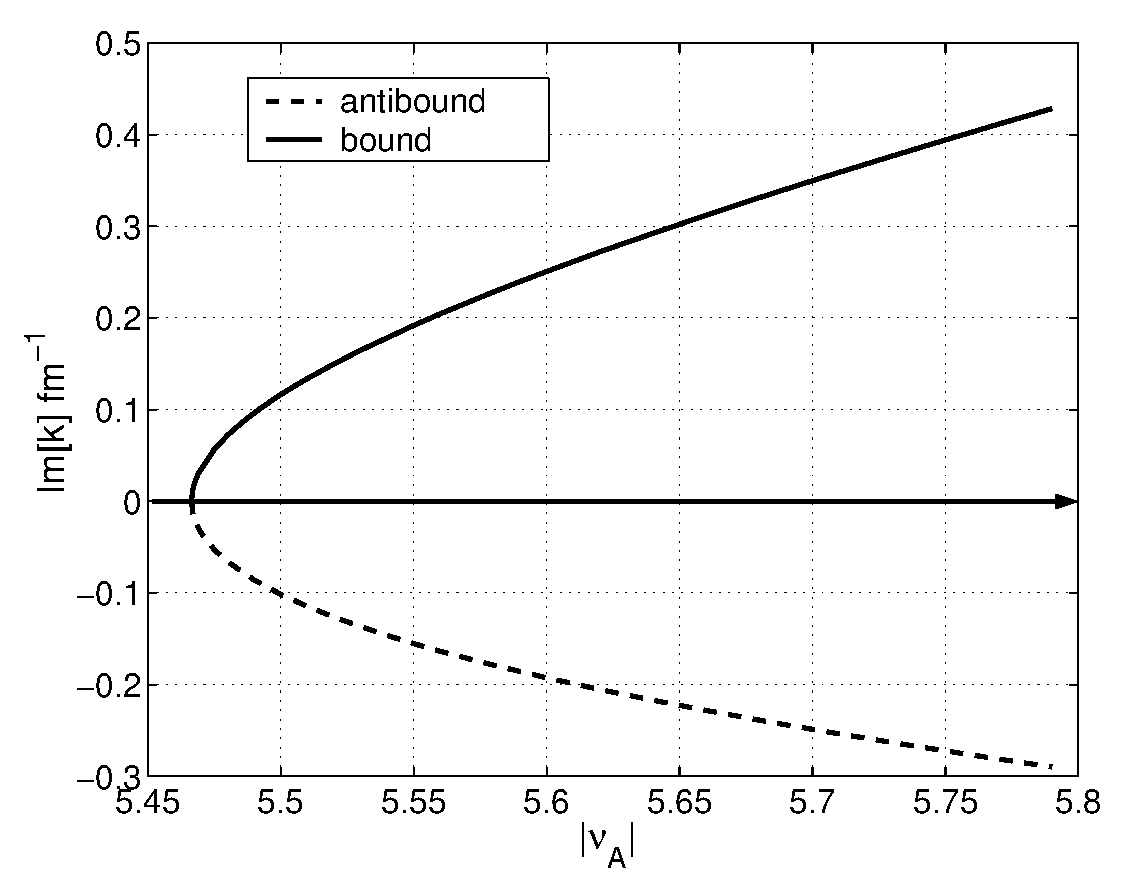
\epsfig{file=figures/fig8.eps}}
\end{center}
\caption{Plot of the bound and antibound state pole trajectory for the $l=1$ component of
Malfliet-Tjon interaction. The location of the poles
along the imaginary $k$-axis is plotted as a function of interaction strength  $\nu_A$. }
\label{fig:antibound}
\end{figure}
In figure~\ref{fig:resonance} a plot of how the $l=1$ bound state in the Malfliet-Tjon potential approaches the scattering 
threshold and develop into decay resonant states for decreasing interaction strength $ \nu_A$ is shown. 
\begin{figure}[hbtp]
\begin{center}
\resizebox{7cm}{6cm}{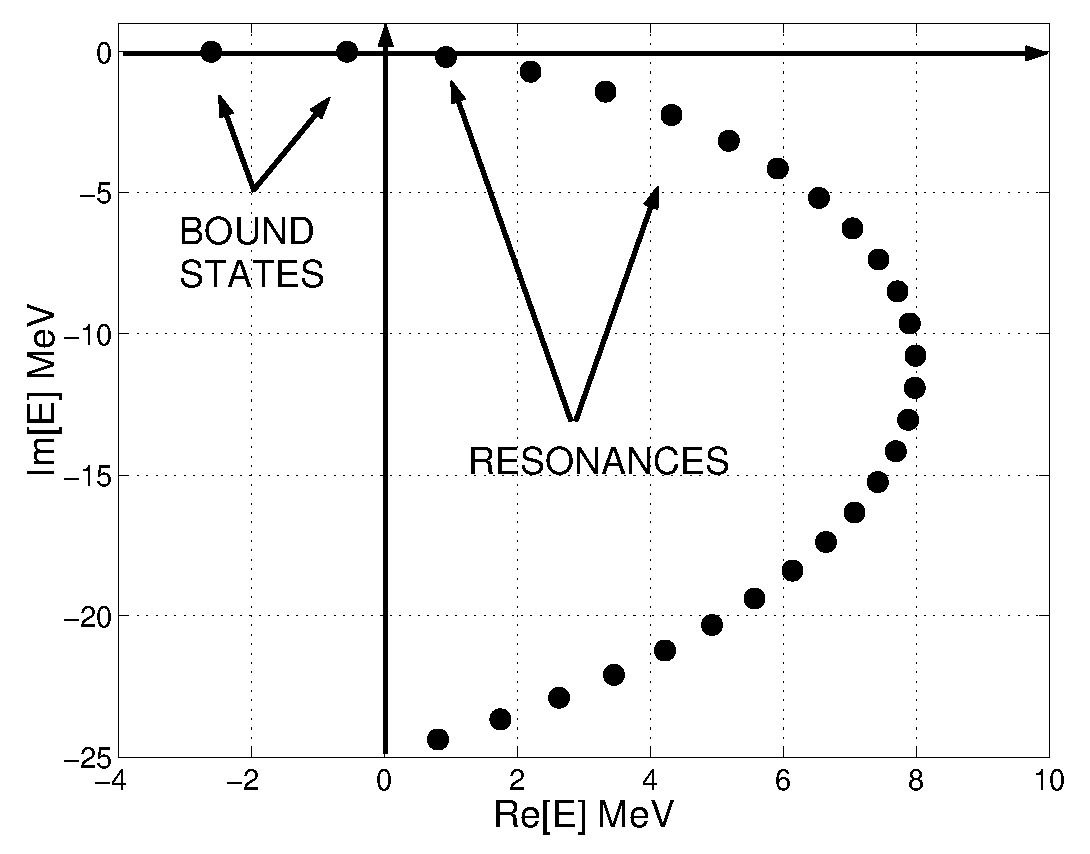
\epsfig{file=figures/fig9.eps}}
\end{center}
\caption{Plot of pole trajectory in the complex energy plane for the $l=1$ partial 
wave solution of the Malfliet-Tjon interaction for
$\nu_A$ varied from $ -5.6 $ to $ -2.9 $ in steps of $0.1$. }
\label{fig:resonance}
\end{figure}
See Paper I for further details on the potential parameters.


% new section
%\section{The generalized complex 
%variational principle; upper and lower bounds 
%for energies in the complex plane} 

% new section
%\section{Two-particle resonances by Sturmian procedures}

\section{Single particle resonances in a deformed field}
\label{sec:deformed}
In this section we will consider formation of resonances in an 
axially deformed field. The study of resonances in deformed fields
has so far only been considered on rare occuations. In Ref.~\cite{deform1}
energy levels and conditions for bound states to become resonances and 
resonances to become bound states were investigated for an 
axially deformed Woods-Saxon potentialm, by solving the 
the radial Schr\"odinger for coupled channels with outgoing asymptotics.
However, the coupled channels method used in Ref.~\cite{deform1} 
does not easily generalize to the non-resonant continuum. This implies
that a complete Berggren basis in a deformed field is difficult to obtain, 
and all evaluated observables will become complex quantities unless
the non-resonant continuum is taken properly into account. 
In Ref.~\cite{deform2} a different approach were considered. Their aim was
to propose a method to obtain scattering wave functions in the vicinity of a 
multi-channel resonance on the real axis. 
Then calculate the phase shifts, and investigate
whether a resonance condition is met. Further this method allows for 
evaluation of observables where the continuum is properly taken into 
account, and they become real quantities. Here we propose 
an alternative method, starting with the momentum space Schr\"odinger equation 
given in equation~(\ref{eq:momspace1}). The obvious advantage of this, is that 
the boundary conditions are automatically built into the integral equations, 
further we will show that a single particle Berggren basis taken 
into account all non-resonant continuum states is possible to obtain
within this approach.

We consider an axially deformed Gaussian potential with no spin and 
tensor components. In spherical coordinates it is given as 
\begin{equation} 
  V(r,\theta) = V_0 \exp\left( -r^2( \alpha \cos^2\theta +\beta \sin^2\theta ) \right) 
  \label{eq:sph1}
\end{equation}  
or in cartesian coordinates, 
\begin{equation} 
  V(x,y,z) = V_0 \exp\left( -\beta (x^2 + y^2)\right) \exp(-\alpha z^2) 
  \label{eq:cartesian1} 
\end{equation}  
here $V_0$ is the strength of the potential and $\alpha $ and $\beta $ are shape
parameters. In the case $ \alpha = \beta $ the potential is just a spherical 
Gaussian potential. In the case $�\alpha > \beta $�the potential field is stretched  
out in the $x,y$-plane, and defines an \emph{oblate}�shape. In the case $\alpha < \beta $ 
the potential field is stretched out in along the $z$-axis, and defines a \emph{prolate} shape. 
Defining a deformation parameter $\delta$ in the following way, 
\begin{equation}
  \delta = 1 - { \alpha \over \beta }, 
\end{equation}
equation~(\ref{eq:sph1}) can be written in the form, 
\begin{equation}
  V(r,\theta;\: \beta, \delta ) = V_0 \exp (-\beta r^2) \exp( \beta \delta r^2 \cos^2\theta) = 
  V(r; \: \beta) D(r,\theta;\: \beta, \delta )
  \label{eq:deform1}
\end{equation}
Here $V(r; \: \beta) $ 
is a spherically symmetric formfactor and $ D(r,\theta;\: \beta, \delta ) $�
a deformation formfactor.
We require that the volume of the central potential, with the shape parameter
$\alpha_0 = \alpha = \beta $, is equal to the volume of the axially 
deformed potential. This gives implies that the shape 
parameters of the non-central and central Gaussian potential satisfy the 
following relation,
\begin{equation}
  \alpha \beta^2 = \alpha_0^3 
\end{equation} 
In figure~\ref{fig:deform1} a plot of the isocurves $V(r,\theta) = 0.5 $ are shown in 
the $x,z$-plane for the deformation parameters $\delta = \pm 0.5$.  $\delta = 0.5 $�
gives 
the shape parameters for the deformed potential $ \alpha = 2^{-2/3}$ 
and $\beta = 2^{1/3}$,
and $\delta = 0.5 $�
gives 
the parameters $ \alpha = (3/2)^{2/3}$ and $\beta = (2/3)^{1/3}$.
Here potential parameters $\alpha_0 = 1$�
and $V_0 = 1$ 
are used. It is
seen that $�\delta = 0.5 $�
corresponds to an \emph{oblate} shape, where the field is
stretched out in the $x,y$-plane. For $\delta = -0.5 $ 
the potential takes a \emph{prolate}
shape, where the field is stretched out along the symmetry axis ($z$-axis). 
\begin{figure}[hbtp]
  \begin{center}
    \resizebox{6cm}{6cm}
	      {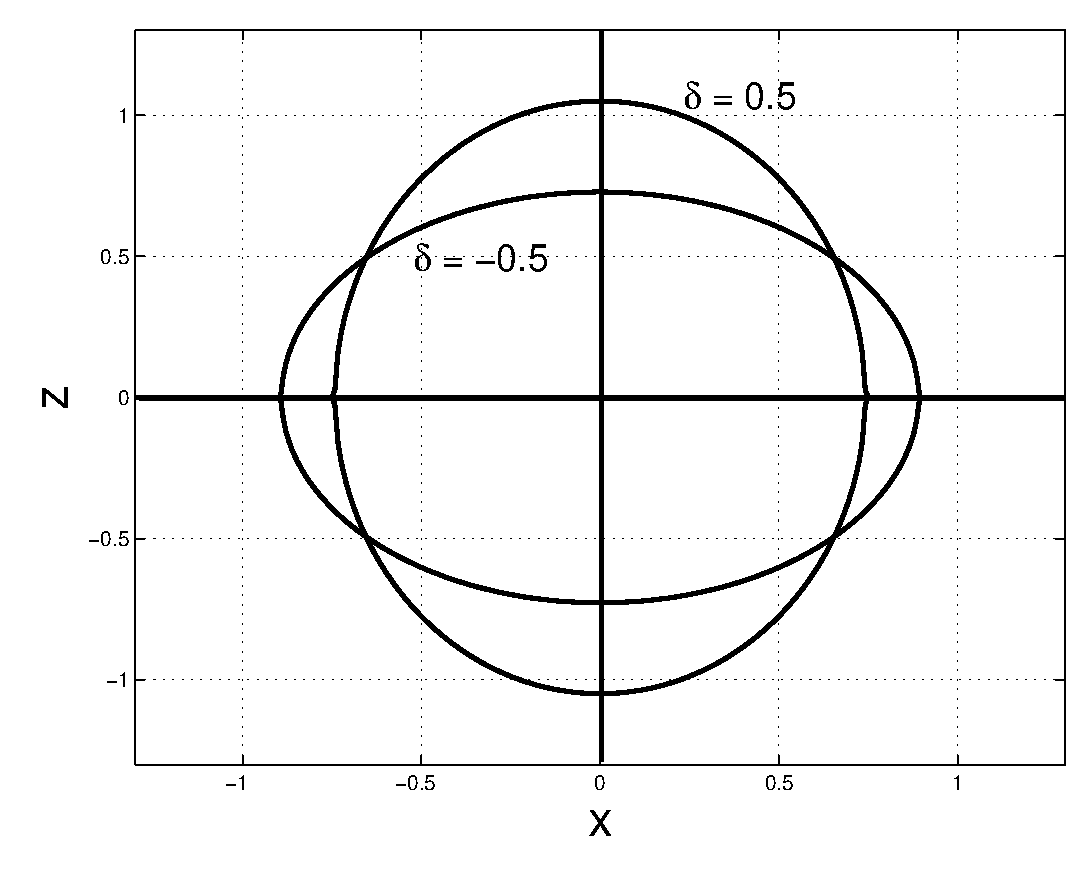
\epsfig{file=figures/deform1.eps}}�
  \end{center}
  \caption{Plot of isocurves $V(r,\theta) = 0.5 $ of the deformed potential for deformation
    $\delta = \pm 0.5 $ with potential strength $V_0 = 1$ in the $x,z$-plane.�
    For the spherically
    symmetric potential a  shape parameter $\alpha_0 = 1 $ were chosen.}
  \label{fig:deform1}
\end{figure}
In order to assess the shape structure in more detail, it is
instructive to study the multipole components of the potential.    
An axially symmetric potential may be expanded in terms
of Legendre polynomials, i.e.  
\begin{equation}
  V(r,\theta) = \sum_\lambda V_\lambda(r) P_\lambda ( \cos\theta) 
  \label{eq:multipoles}
\end{equation}
the multipole components are then given by the  integrals 
\begin{equation}
  V_\lambda(r) = { (2\lambda + 1) \over 2} V_0 \exp (-\beta r^2) \int_{-1}^1 dx \:
  \exp( \beta \delta r^2 x^2 ) P_\lambda(x) 
\end{equation}
Here it is explicitly seen that only \emph{even} multipoles give non-vanishing 
contributions, since the Legendre polynomials have the 
property 
\[
�P_\lambda(-x) = (-1)^\lambda P_\lambda(x),
\]
and the potential is an even function in $x$. 
\begin{figure}[hbtp]
  \begin{center}
    \resizebox{16cm}{8cm}{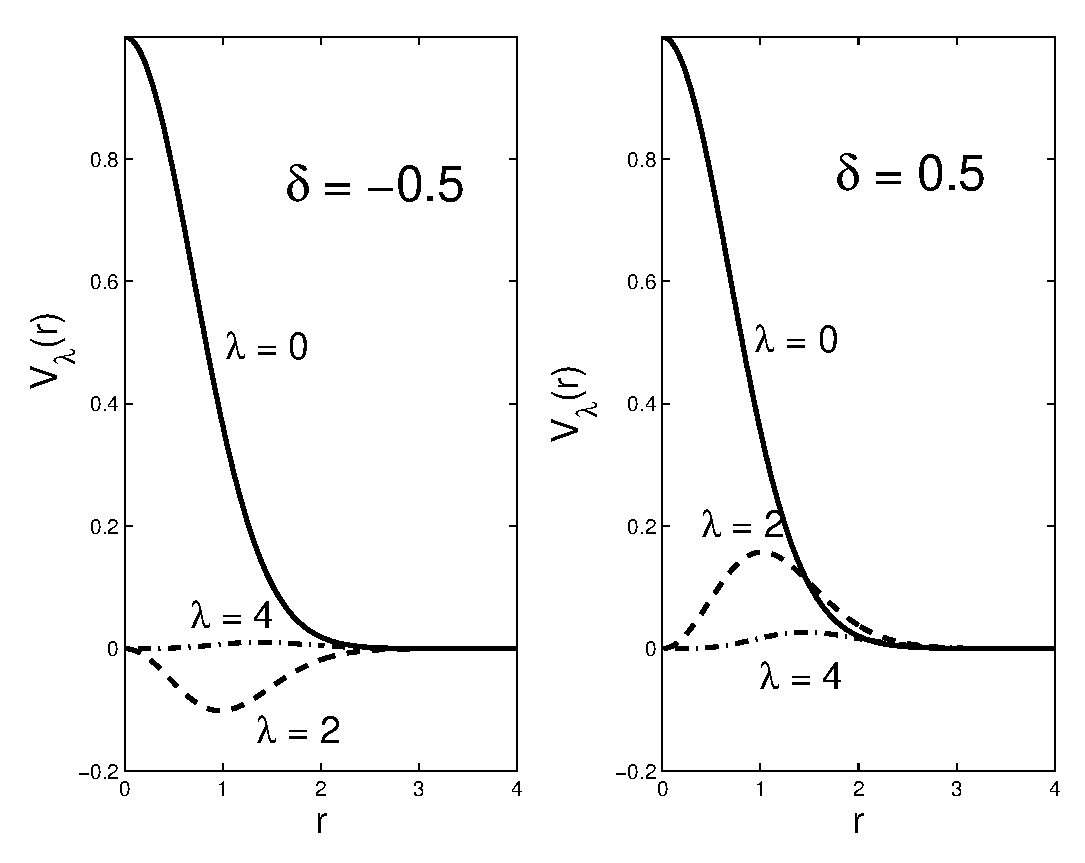
\epsfig{file=figures/multi_poles.eps}}
  \end{center}
  \caption{Plot of $\lambda = 0,2,4$ multipoles of the Gaussian potential 
    with deformation parameters $\delta = 0.5$ (right plot) and $\delta = -0.5$  
    (left plot)  and $\alpha_0 = 1 $}
\label{fig:multi1}
\end{figure}
Figure~\ref{fig:multi1} gives a plot of the 
$\lambda = 0,2,4$ multipoles of the Gaussian potential  
with deformation parameters $\delta = \pm 0.5$. It is seen that the radial monopole 
distribution is more or less identical for $\delta = 0.5 $ and $\delta = -0.5$. 
From the  volume conservation imposed on the deformed potential, it 
follows that the volume of the monopole part of the potential is independent of the 
deformation parameter $\delta $. 
This is easy to show, since  $P_\lambda(\cos\theta) = Y_{\lambda 0}(\theta, \varphi)$
and using the well known property of the spherical harmonics (see e.g. \cite{varshalovich} ), 
\begin{equation}
  \int d\hat{r} Y_{lm}(\hat{r}) = \sqrt{4 \pi}\delta_{l,0}\delta_{m,0}
\end{equation}
from which it follows directly, 
\begin{equation}
\int dV\: V({\bf r}) = \int_0^\infty dr\: r^2V_{\lambda = 0}(r)
\end{equation}
Further it is seen that the deformed Gaussian potential 
is nearly a pure quadrupole deformation, since the $\lambda =4$ 
multipole is almost vanishing in both cases. This may be understood
from considering the exponent of the deformed formfactor in equation~(\ref{eq:deform1}),
which can be rewrittin in terms of the $ Y_{20}(\hat{r}) $ spherical harmonic.

Having discussed the shape and multipoles of the deformed Gaussian potential, 
we now turn to the acually solution of the Schr\"odinger equation for 
this potential. We wish to solve the 
momentum space Schr\"odinger equation given in equation~(\ref{eq:momspace1}).
The Fourier transformation of the deformed 
Gaussian potential in equation~(\ref{eq:cartesian1})
is, 
\begin{eqnarray}
  \nonumber
  V(q_x,q_y,q_z) & = &  {V_0 \over (2\pi)^3 }\int dx \:dy \:dz\: 
  \exp\left( i( q_x x +q_y y +q_z z) \right) 
  \exp\left( -\beta (x^2 + y^2) -\alpha z^2 \right) \\ 
  &  = &{V_0 \over 8 \pi^{3/2} \beta \alpha^{1/2}�}
  \exp\left( -{1\over 4 \beta}(q_x^2 +q_y^2) \right)   
  \exp\left( -{1\over 4 \alpha} q_z^2 \right)
\end{eqnarray}
here $q_i= k_i - k_i',\: i = x,y,z$. In terms of spherical coordinates $k,\theta, \varphi�$  
the potential takes the form, 
\begin{eqnarray}
  \nonumber
  V({\bf k},{\bf k}')&  = & {V_0 \over 8 \pi^{3/2} \beta \alpha^{1/2}�}
  \exp\left( -{1\over 4 \beta} ( k^2 \sin^2\theta + {k'}^2\sin^2\theta')
  -{1\over 4 \alpha} ( k^2 \cos^2\theta - {k'}^2\cos^2\theta')^2\right) \\
  & \times & \exp\left( -{1\over 4 \beta } kk'\sin\theta\sin\theta' \cos\left( \varphi - \varphi'\right) \right)
  \label{eq:sph2}
\end{eqnarray} 
due to axial symmetry the  dependence of the potential 
on the azimuthal angles $\varphi, \varphi' $ is only the difference 
$�\omega = \varphi - \varphi'$. The potential may therefore be expanded in 
a complete set of harmonics, i.e. 
\begin{equation}
  V( {\bf k}, {\bf k'}) = \sum_{\mu = -\infty}^\infty V_{\mu}(\tilde{k}, \tilde{k}') \exp(i \mu \omega), 
  \label{eq:pot_exp1}
\end{equation}
here $\tilde{k} = k,\theta $. 
The harmonics $\exp ( i\mu \omega )$ obey the orthogonality relation 
\begin{equation}
  \int_{-\pi}^\pi d\omega \: \exp (-i\mu \omega) \exp( i\mu'\omega) = 2\pi \delta_{\mu,\mu'}
\end{equation}
the $\mu$'th harmonic of the potential is therefore given by the integral
\begin{equation}
  V_\mu( \tilde{k},\tilde{k}') = 
    {1 \over 2\pi} \int_{-\pi}^\pi d\omega \:\exp(-i\mu \omega) V({\bf k},{\bf k}')
\end{equation}
From equation~(\ref{eq:sph2}) it is seen, that for the integral over $\omega $, 
we have to consider the following integral, 
\begin{equation}
  I_{\mu}(y) = {1 \over 2\pi} \int_{-\pi}^\pi d\omega \:\exp(-i\mu \omega) 
  \exp( y \cos\omega ) = {1\over \pi} \int_0^\pi d\omega \: \cos( \mu \omega) \exp(y \cos\omega ) 
  \label{eq:bessel1}
\end{equation}
where we have introduced the variable 
\[
y = {1\over 2\beta } kk'\sin\theta\sin\theta'.
\]
The integral in equation~(\ref{eq:bessel1}) is just the definition of the modified Bessel 
function of the 1'st kind (see e.g. \cite{stegun}). 
The $\mu$'th harmonic of the potential is analytic form given by, 
\begin{eqnarray}
  \nonumber
  V_\mu( \tilde{k},\tilde{k}') = {V_0 \over 8 \pi^{3/2} \beta \alpha^{1/2}�} \times  \\
  \exp\left( -{1\over 4 \beta} ( k^2 \sin^2\theta - {k'}^2\sin^2\theta')^2
  -{1\over 4 \alpha} ( k^2 \cos^2\theta - {k'}^2\cos^2\theta')^2\right) 
  \exp(-y) I_{\mu}(y)
\end{eqnarray}
Inserting the expansion of the potential given in equation~(\ref{eq:pot_exp1}) into 
the momentum space Schr\"odinger equation~(\ref{eq:momspace1}) and projecting 
the equation on the harmoncis $\exp ( i\mu \omega )$, the three-dimensional 
integral equation has been reduced to an infinite set of two-dimensional 
integral equations. The $\mu$'th integral equation is easily solved as
a matrix diagonalization problem with dimension $N_r\times N_\theta $. 
Where $N_r$ is the number of integration points for the radial integral 
and $N_\theta$ is the number of integration points for the angle integral. The
Schr\"odinger equation can be further reduced to a coupled set of one-dimensional
integral equation by projecting on spherical harmonics (see equation~(\ref{eq:part_wave2})). 
The angular momentum projected potential in equation~(\ref{eq:sph2}) then  takes the form, 
\begin{eqnarray}
  \nonumber
  V_{lm, l'm'}(k,k') = \int \mathrm{d}{\hat{k}} \int \mathrm{d}{\hat{k}'}\: 
  Y_{lm}^*(\hat{k})\left\{ \sum_{\mu = -\infty}^\infty V_{\mu}(\tilde{k}, \tilde{k}') 
  \exp(i \mu \omega)\right\}   Y_{l'm'}(\hat{k}') \\
  = 2\pi \int_0^\pi d\theta \: \sin\theta \int_0^\pi d\theta' \: \sin\theta' 
  \bar{P}_{lm}(\cos\theta) V_{m}(\tilde{k}, \tilde{k}')  \bar{P}_{l'm}(\cos\theta') \:\delta_{m,m'}  
  \label{eq:pot_exp2}
\end{eqnarray}
where $�\bar{P}_{lm}(x)$ are the normalized associated Legendre polynomials, 
\begin{equation}
  \bar{P}_{lm}(x) = \left\{ { 2l + 1 (l-m)! \over 2 (l+m)! }\right\}^{1/2}P_{lm}(x).
\end{equation}
We wish to study the formation of resonances in the deformed Gaussian potential by 
the contour deformation method. 
The 1-dimensional coupled integral equation are then analytically continued
from the physical to the non-physical energy sheet by distorting the integration contour. 
Choosing a suitable inversion symmetric 
contour $L^+$, discussed in the previous section, we end up with the 
analytically continued coupled integral equations for the axially deformed Gaussian potential, 
\begin{equation}
  \left( {\hbar^2 \over 2\mu } k^2 - E_{nlm}\right) \psi_{nlm}(k) =  
  -\sum_{l'} \int_{L^+} dk' {k'}^2 V_{lm, l'm}(k,k') \psi_{nl'm}(k') 
  \label{eq:part_wave3}
\end{equation}
As a case study we consider a Gaussian potential which in the spherically 
symmetric case reproduce the $J^\pi={3/2^{-}_1} $ resonance in $^5$He. 
The  $J^\pi={3/2^{-}_1}$ resonance, to be associated with the single-particle orbit 
$p_{3/2}$, is experimentally 
known to have a width of $\Gamma \approx 0.60$ MeV.
Using the following parameters for the sperically symmetric Gaussian given in 
equation~(\ref{eq:sph1}),
\begin{equation}
  V_0 = -53.5 \mathrm{MeV}, \:\: \alpha_0 = 0.188 \mathrm{fm}^{-2}
\end{equation}
the Gaussian potential supports a bound state for 
the $l^\pi = 0^+$ channel with energy $E = -14.9044 �$MeV, 
and a resonance for the $l^\pi = 1^-$ channel with energy 
$E = 0.7268  -0.3096i $MeV. Here the nucleon spin $s=1/2$�is neglected
since the energy levels are degenerate for $ j = l \pm 1/2 $, which 
follows from the spin independence of the Gaussian potential.
Table~\ref{tab:deform1} gives the convergence of the $m^\pi = 0^+$ 
ground state for deformation parameters $ \delta = \pm 0.9$. It is seen that
the deformation $\delta = 0.9$ affects the bound state the most, and 
the ground state becomes much more less bound $ E = -12.1 $MeV, 
for the prolate deformation. 
On the other hand, the oblate deformation $\delta = -0.9$ has little effect
on the ground state energy $E = -14.7$MeV.  
\begin{table}[htbp]
  \begin{center}
  \begin{tabular}{ccccc}
    \hline
    \multicolumn{1}{c}{} & \multicolumn{2}{c}{$\delta = 0.9 $} 
    & \multicolumn{2}{c}{$\delta = -0.9$} \\
    \hline
    \multicolumn{1}{c}{$l_{\mathrm{max}}$} &
      \multicolumn{1}{c}{Re[E]} & \multicolumn{1}{c}{Im[E]} &
      \multicolumn{1}{c}{Re[E]} & \multicolumn{1}{c}{Im[E]} \\
    \hline
    0 &  -10.5843 & 0.&  -14.4816 & 0.\\
    2 &  -11.9041 & 0.&  -14.6533 & 0.\\
    4 &  -12.0741 & 0.&  -14.6551 & 0.\\
    6 &  -12.0953 & 0.&  -14.6551 & 0.\\
    8 &  -12.0979 & 0.&  -14.6551 & 0.\\ 
    10 & -12.0983 & 0.&  -14.6551 & 0.\\
    \hline
  \end{tabular}
  \caption{Convergence of groundstate, $m^\pi = 0^+$, for deformation
    parameters  $\delta = \pm 0.9$ as the number of partial waves increases.
    In the spherically symmetric case $\delta = 0$ the  $l^\pi=0^+$ Gaussian potential 
    supports a bound state at energy $ E = -14.9044 $MeV. }
  \label{tab:deform1}
  \end{center}
\end{table}
This may be understood by considering the monopole term of the potential, 
which is the main component in the multipole expansion in equation~(\ref{eq:multipoles}).
In figure~\ref{fig:monopole} a plot of the monopole part of the Gaussian 
potential with deformation parameters $\delta = \pm 0.9$ is given, together with a plot 
of the spherically symmetric potential. It is
seen that the monopole term for the $\delta = -0.9$�potential is more or less identical 
to the spherically symmetric potential (slightly less attractive), 
on the other hand the monopole 
term for the $\delta = 0.9�$ potential is less attractive for small radii, but
more attractive at large distances.  From this one may conclude that the 
ground state of the $\delta = -0.9$ 
potential will be more bound than for the $\delta = 0.9$ potential, since 
the ground state is deeply bound and the wave function will be
mainly located in the interior part of the potential.
\begin{figure}
  \begin{center}
    \resizebox{10cm}{8cm}{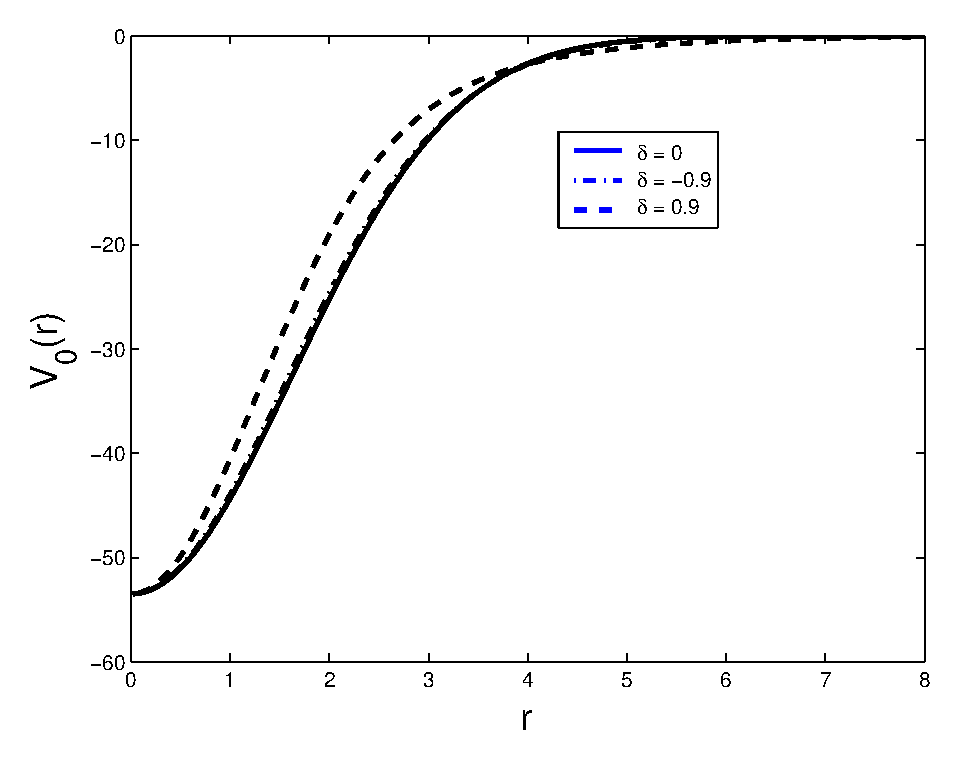
\epsfig{file=figures/monopole.eps}}
  \end{center}
  \caption{Plot of the monopole part  of the Gaussian potential 
    with deformation parameters $\delta = 0$ and $\delta = \pm 0.9$.}
  \label{fig:monopole}
\end{figure}


The resonant orbit $l^\pi = 1^-$ in the spherically symmetric 
potential is split into two non-degenerate orbits ( $m^\pi = 0^- $ and $ m^\pi  = 1^-$) 
in the case of an axially symmetric deformation. This is a 
characteristic of axially deformed potentials.
Table~\ref{tab:deform2} gives the convergence of the $m^\pi = 0^-$ and  
$m^\pi = 1^-$ excited negative parity states in the Gaussian potential
for deformation parameters $ \delta = \pm 0.5$. In all cases a satisfactory 
convergence is obtained with $l_{\mathrm{max}} = 5$.�For the states 
with angular momentum projection along the $z$-axis ( $ m = 0$ ), it is
seen that for $\delta = 0.5$, ( prolate deformation ), the $ l^\pi = 1^-$ state
has become a bound state with energy $�E = -0.680 $MeV. 
For zero angular momentum projection, the particle moves in an orbit
making $ \theta = 0$ degrees with the $z$-axis. So in the case of a prolate deformation, 
where the field is stretched out along the $z$-axis, a particle moving in this
orbit will ``feel'' the field more strongly than compared with the spherically symmetric 
field, and it will become more bound. This explains also why the particle 
with $m=0$ becomes more unbound in the case of the oblate deformation $\delta = -0.5$,
see Columns 6 and 7 of table~\ref{tab:deform2}.  
\begin{table}[htbp]
  \begin{center}
  \begin{tabular}{ccccccccc}
    \hline
    \multicolumn{1}{c}{} & \multicolumn{4}{c}{$\delta = 0.5 $} 
    & \multicolumn{4}{c}{$\delta = -0.5$} \\
    \hline
    \multicolumn{1}{c}{} & \multicolumn{2}{c}{$m^\pi = 0^- $} 
    & \multicolumn{2}{c}{$ m^\pi = 1^- $} 
    & \multicolumn{2}{c}{$m^\pi = 0^- $} 
    & \multicolumn{2}{c}{$ m^\pi = 1^- $} \\
    \hline
    \multicolumn{1}{c}{$l_{\mathrm{max}}$} &
    \multicolumn{1}{c}{Re[E]} & \multicolumn{1}{c}{Im[E]} &
    \multicolumn{1}{c}{Re[E]} & \multicolumn{1}{c}{Im[E]} &
    \multicolumn{1}{c}{Re[E]} & \multicolumn{1}{c}{Im[E]} &
    \multicolumn{1}{c}{Re[E]} & \multicolumn{1}{c}{Im[E]} \\
    \hline
    1 &   -0.5282 & 0. &  1.4865 & -1.0177 &  1.5402 & -1.0701 &  0.3815 & -0.1139 \\
    3 &   -0.6772 & 0. &  1.4419 & -0.9631 &  1.5170 & -1.0404 &  0.3602 & -0.1042 \\
    5 &   -0.6802 & 0. &  1.4410 & -0.9621 &  1.5168 & -1.0402 &  0.3601 & -0.1041 \\
    7 &   -0.6803 & 0. &  1.4410 & -0.9620 &  1.5168 & -1.0402 &  0.3601 & -0.1041 \\
    9 &   -0.6803 & 0. &  1.4410 & -0.9620 &  1.5168 & -1.0402 & 0.3601 & -0.1041  \\
    \hline
  \end{tabular}
  \caption{Convergence of the $m^\pi = 0^-$ and $m^\pi = 1^-$ states, for deformation
    parameters  $\delta = \pm 0.5$ with increasing number of partial waves.
    In the spherically symmetric case ($\delta = 0$) the  $l^\pi=1^-$ Gaussian potential 
    supports a resonance state at energy $ E = 0.7268  -0.3096i $MeV.}
\label{tab:deform2}
\end{center}
\end{table}

\begin{table}[htbp]
  \begin{center}
  \begin{tabular}{ccccccccc}
    \hline
    \multicolumn{1}{c}{} & \multicolumn{4}{c}{$\delta = 0.5 $} 
    & \multicolumn{4}{c}{$\delta = -0.5$} \\
    \hline
    \multicolumn{1}{c}{} & \multicolumn{2}{c}{$m^\pi = 0^- $} 
    & \multicolumn{2}{c}{$ m^\pi = 1^- $} 
    & \multicolumn{2}{c}{$m^\pi = 0^- $} 
    & \multicolumn{2}{c}{$ m^\pi = 1^- $} \\
    \hline
    \multicolumn{1}{c}{$l$} &
    \multicolumn{1}{c}{Re[$\psi_{l}^2$ ]} & \multicolumn{1}{c}{Im[$\psi_{l}^2$]} &
    \multicolumn{1}{c}{Re[$\psi_{l}^2$ ]} & \multicolumn{1}{c}{Im[$\psi_{l}^2$]} &
    \multicolumn{1}{c}{Re[$\psi_{l}^2$ ]} & \multicolumn{1}{c}{Im[$\psi_{l}^2$]} &
    \multicolumn{1}{c}{Re[$\psi_{l}^2$ ]} & \multicolumn{1}{c}{Im[$\psi_{l}^2$]} \\
    \hline
    1 &   0.9947 & 0. & 0.9982 & 2.31E-03& 0.9992 & 1.1E-03 & 0.9993 & 3.E-04 \\ 
    3 &   5.7E-03&0. & 1.8E-03 &-2.3E-03& 8.E-04&-1.1E-03& 7.E-04 &-3.E-04 \\
    5 &   5.E-05 & 0. &2.E-05  &-2.E-05 & 3.E-06&-3.E-06& 2.E-06 &-9.E-07 \\
    7 &   6.E-07 & 0. &3.E-07  &-2.E-07 & 2.E-08&-1.E-08& 9.E-09 &-4.E-09 \\
    9 &   8.E-09 & 0. &4.E-09  &-3.E-09 & 9.E-11&-7.E-11& 4.E-11 &-2.E-11 \\
    \hline
  \end{tabular}
  \caption{Convergence of the $m^\pi = 0^-$ and $m^\pi = 1^-$ states, for deformation
    parameters  $\delta = \pm 0.5$ with increasing number of partial waves.
    In the spherically symmetric case ($\delta = 0$) the  $l^\pi=1^-$ Gaussian potential 
    supports a resonance state at energy $ E = 0.7268  -0.3096i $MeV.}
\label{tab:deform3}
\end{center}
\end{table}
For the $m=1$ case the opposite
takes place. In the case of $\delta = 0.5$ the particle becomes more unbound, 
while in the of $\delta = -0.5$ the particle becomes more bound. By considering 
the dipole ($l=1$) term of the wave function, the particle moves in 
an orbit making $\theta = \pi/4$�degrees with the $z$-axis. From this
it may be understood that particle gains more binding in the case of 
an oblate deformation $\delta = -0.5$ and becomes more unphysical in the 
opposite case $\delta = 0.5$ 
( see columns 4,5,8 and 9 of table~\ref{tab:deform2}).

In table~\ref{tab:deform3} the squared amplitudes of the wave functions are given
for each partial wave $l$. It is seen that in all cases that the 
squared amplitudes for the $l=1$ component of the total wave function, 
is nearly equal to the norm of the total wave function, while
all other partial wave amplitudes are vanishing. In this sense one may 
say that the orbital angular momentum is approximatetly a ``good'' quantum number. 

In figure~(\ref{fig:0plus}) a plot of the bound state energy of the $m^\pi 0= 0^+$ 
state are given for the deformation parameter $\delta $ 
taking values between $-0.9$�and $0.9$. It is seen that the position of the
bound state varies much more strongly for a prolate deformation ($\delta > 0$), than 
for an oblate deformation. 
\begin{figure}[hbtp]
  \begin{center}
    \resizebox{16cm}{8cm}{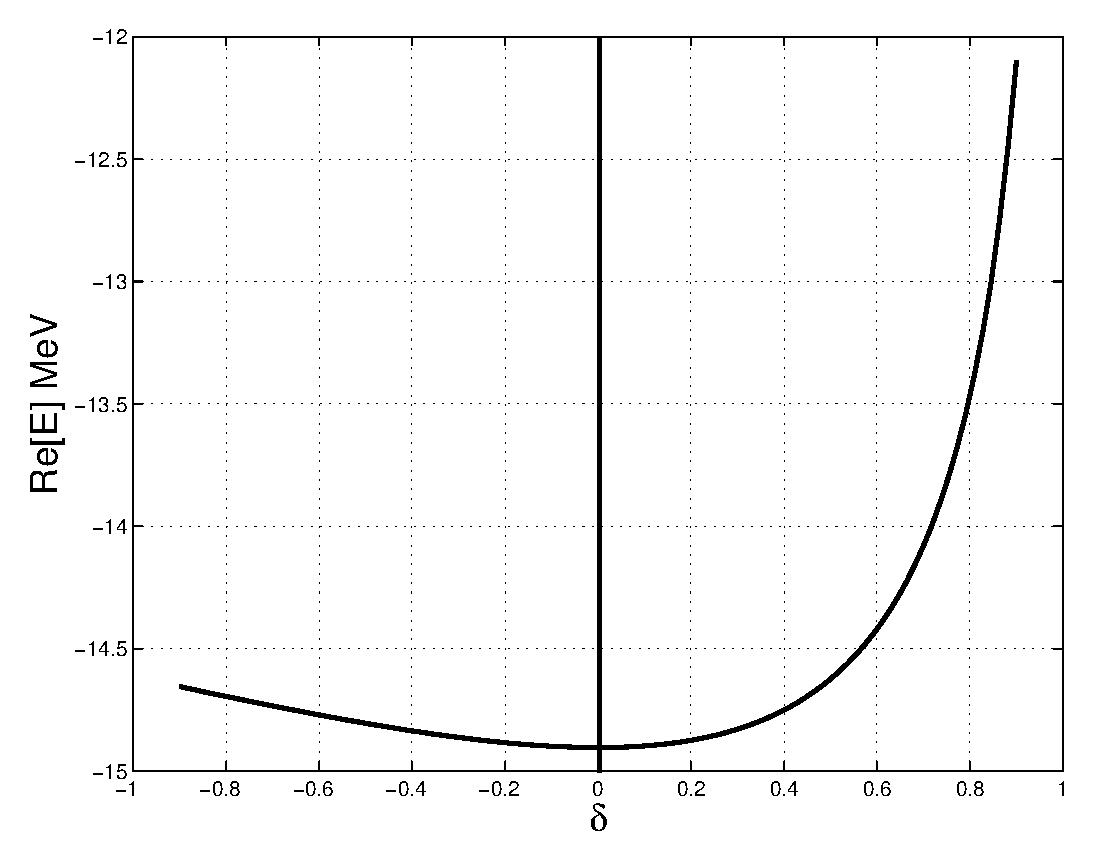
\epsfig{file=figures/0plus.eps}}
  \end{center}
  \caption{Bound state trajectory for the $m^\pi = 0^+$ state in the deformed 
  Gaussian potential. Energy is plotted as function of deformation parameter $\delta$.}
\label{fig:0plus}
\end{figure}

In figure~(\ref{fig:0minus}) a plot of the real and imaginary parts of the $m^\pi = 0^-$ 
state are given for the deformation parameter $\delta $ 
taking values between $-0.9$�and $0.9$. Here it is seen that resonance in the 
$\delta =0$ becomes a bound state for $\delta > 0.3�$. For $\delta < 0$ the resonance
becomes more unphysical with $\delta$. 
\begin{figure}[hbtp]
  \begin{center}
    \resizebox{16cm}{8cm}{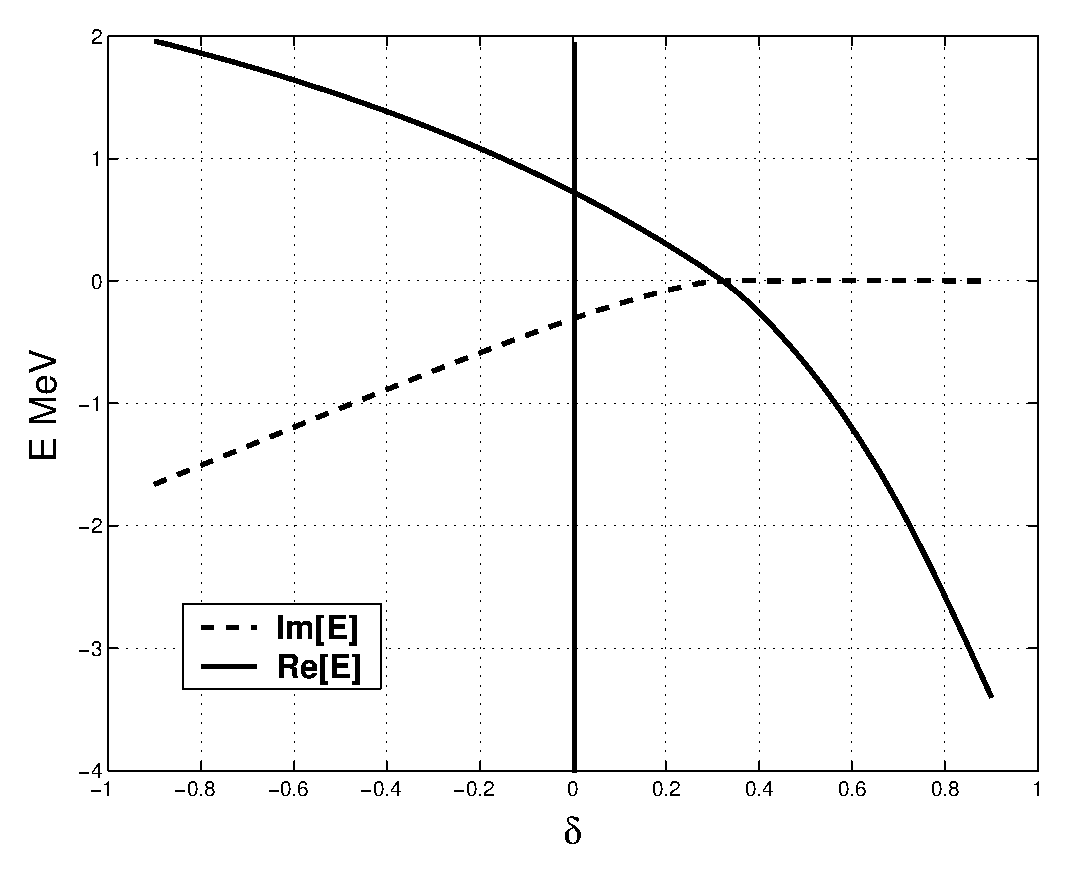
\epsfig{file=figures/0minus.eps}}
  \end{center}
  \caption{Real and imaginary part of the $m^\pi = 0^-$ state energy in the deformed 
    Gaussian potential as the deformation parameter $\delta $ is varied between $-0.9$�and $0.9$.}
  \label{fig:0minus}
\end{figure}


In figure~(\ref{fig:1minus}) a plot of the real and imaginary parts of the $m^\pi = 1^-$ 
state are given for the deformation parameter $\delta $ 
taking values between $-0.9$�and $0.9$. Here the resonance state never becomes a
bound state for $\delta \in (-0.9,0.9)$. For $\delta \in ( -0.9,0.2) $ 
the resonance display a weak variation from the $\delta = 0$ resonance. On the
other hand, as $\delta \rightarrow 0.9 $ the imaginary part of the energy
dives into the lower half complex energy plane, and the resonance
state becomes strongly unphysical.
\begin{figure}[hbtp]
  \begin{center}
    \resizebox{16cm}{8cm}{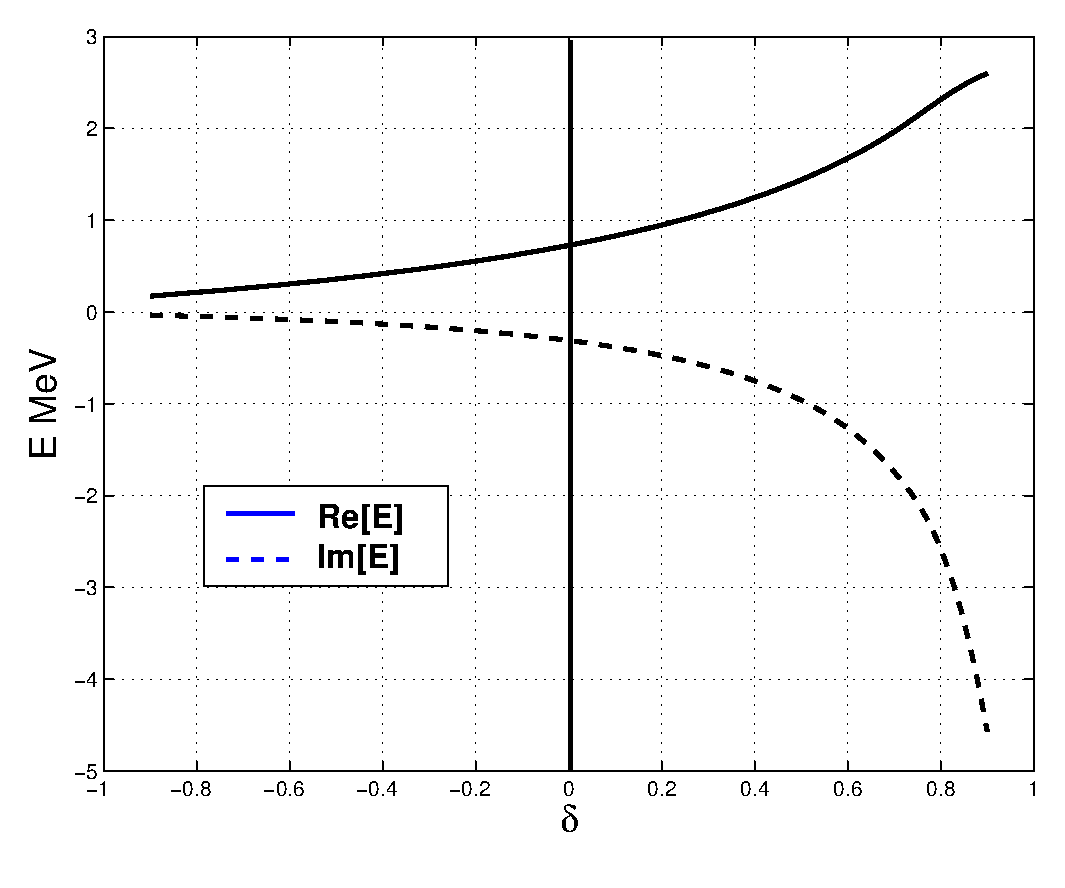
\epsfig{file=figures/1minus.eps}}
  \end{center}
  \caption{Real and imaginary part of the $m^\pi = 1^-$ state energy in the deformed 
    Gaussian potential as the deformation parameter $\delta $ is varied between $-0.9$�and $0.9$.}
  \label{fig:1minus}
\end{figure}

In figure~(\ref{fig:combined}) a combined plot of the real and imaginary parts of the $m^\pi = 0^-$ 
and $ m^\pi = 1^-$�states are given for the deformation parameter $\delta $ 
taking values between $-0.9$�and $0.9$. Here the splitting of the $l^\pi = 1^-$ 
resonant level with respect to the angular momentum projection $m$ is clearly seen.
\begin{figure}[hbtp]
  \begin{center}
    \resizebox{16cm}{8cm}{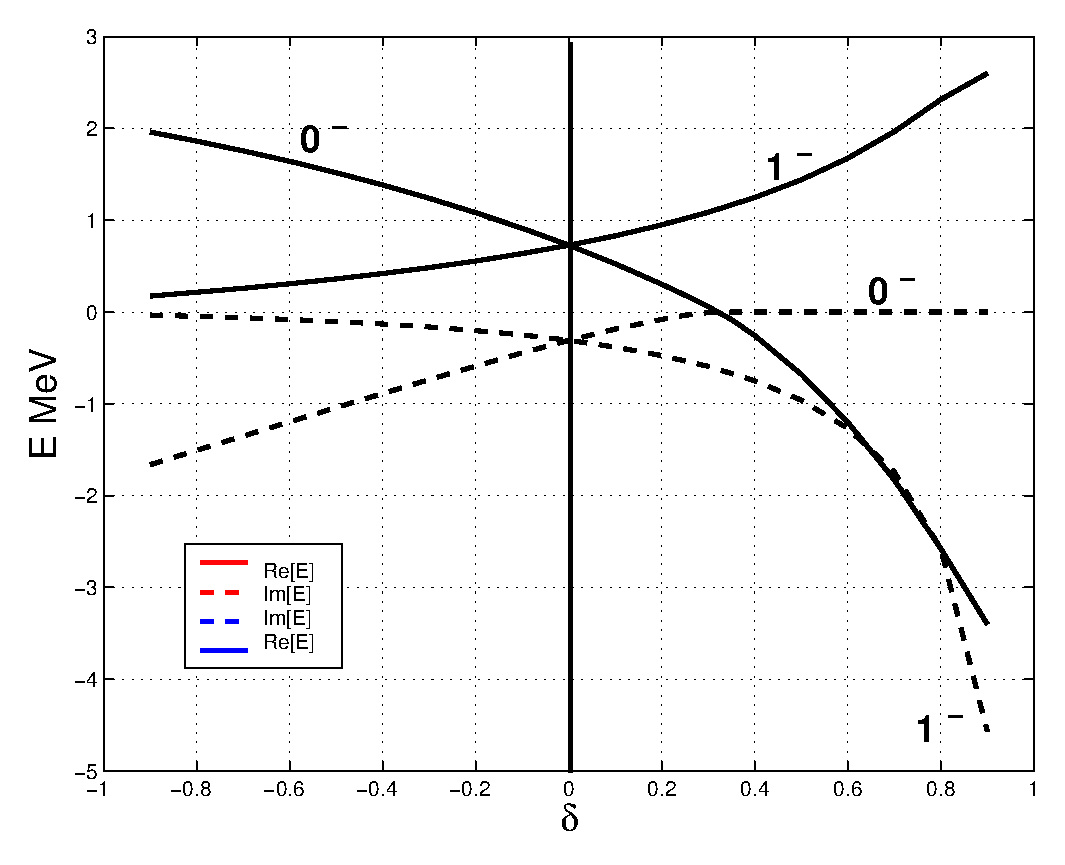
\epsfig{file=figures/deform_minus.eps}}
  \end{center}
  \caption{Real and imaginary part of the $m^\pi = 1^-$ state energy in the deformed 
    Gaussian potential as the deformation parameter $\delta $ is varied between $-0.9$�and $0.9$.}
  \label{fig:combined}
\end{figure}

% new section^
\section{Two-particle resonances and bound states embedded in the continuum in complex potentials} 
\label{sec:optical}
CDM has a number of different applications, in this section
scattering from a complex Malfliet-Tjon interaction 
describing absorbtive and emitting processes is considered. 
\footnote{See Paper I for a detailed analysis of the 
structure of the Malfliet-Tjon potential in momentum space, the relevant 
equations to be solved and the bound, anti-bound and resonant pole distributions 
as funtion of the interaction strength.}
Complex potentials have commonly been used in optical potential models 
in nuclear and particle physics. Inelastic scattering where the conservation 
of flux is broken due to the possibility of the particle to 
be ejected to other exit channels or particles to emerge from them, may 
be taken into account by a complex absorbing or emitting potentials respectively. 
Another application of complex potentials, is the nucleon-antinucleon scattering,
in which a short range complex annihilation potential may describe how
bound- and resonant states are formed such systems. 

In letting the interaction strengths be generalized to the complex plane 
the Schr\"odinger equation 
becomes a non-hermitian eigenvalue problem from the very beginning, and 
the eigenvalues will in general 
become complex. See Refs.~\cite{kukulin, kok} for a more rigorous 
discussion of complex interactions. Below follows an illustration that 
CDM gives accurate calculation 
of the complete energy spectrum for complex interactions.  
The pole 
trajectories are studied by varying the absorbtive 
and emittive strength of the interaction. 

In the case of the Malfliet-Tjon interaction two cases are studied. 
First the attractive strength, $ V_A  \rightarrow (1+\eta i)V_A $, is scaled 
by a complex constant $ 1 + \eta�i$ 
keeping the repulsive strength $V_R$  real. 
Since the attractive strength $V_A$ is a negative quantity, 
absorbtive scattering takes place for $ \eta > 0�$ while
emittive scattering takes place for $ \eta < 0$. 
Secondly  both the attractive and repulsive interaction
strengths are scaled, i.e. $ V  \rightarrow (1+\eta i)V$. 
Starting with $\nu_A = -5 $,
 so for $ \eta = 0 $ a resonance at
$ E = 5.1804 -3.1555i $ MeV corresponding to a pole at $ k = 0.3682 - 0.1033i \: \mathrm{fm}^{-1}�$ 
in the complex $k$-plane appears (see Paper I)
\footnote{Here $ V_A = \nu_A\times \hbar c�$, see Paper I for more details.}.
In figure~\ref{fig:optical1} a plot of 
the pole trajectory for varying $\eta $ 
is given, keeping $\nu_A$ fixed. An imaginary part is added to the attractive
strength $V_A$ while $V_R$ is kept real. 
\begin{figure}[hbtp]
\begin{center}
\resizebox{9cm}{7cm}{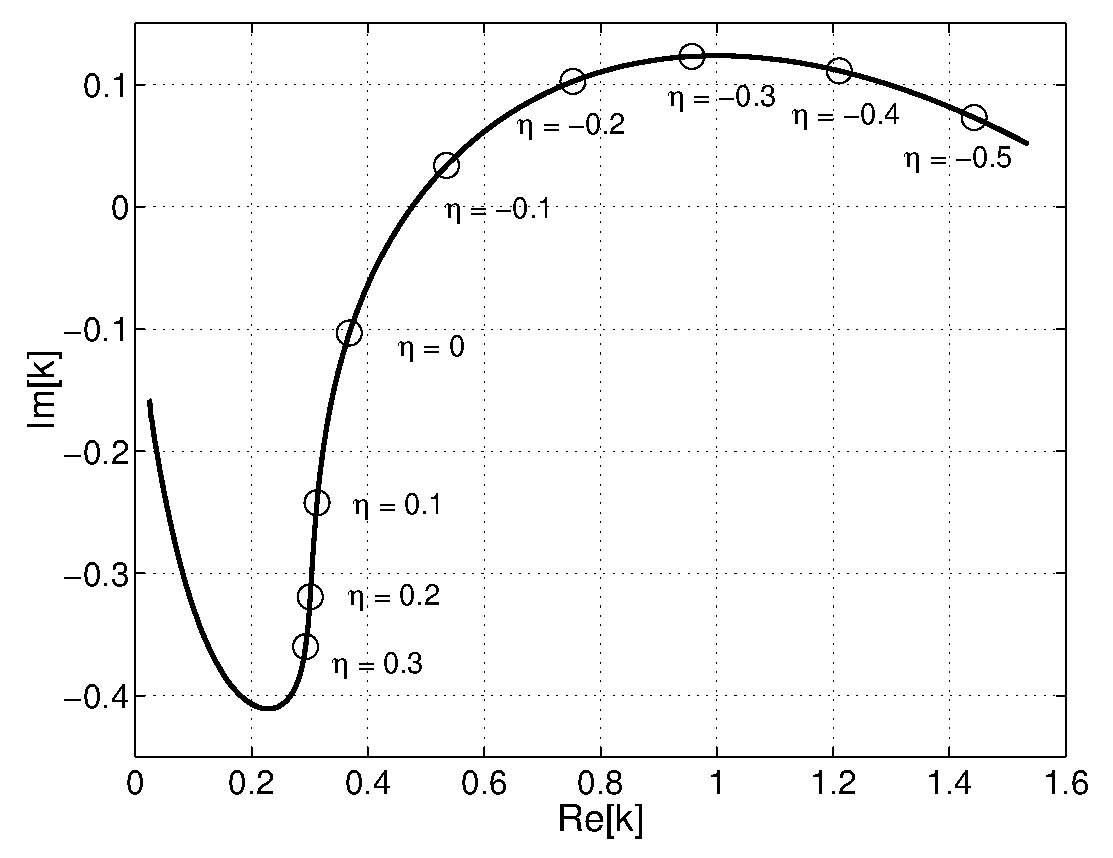
\epsfig{file=figures/optical.eps}}
\end{center}
\caption{Pole trajectory of the $l=1$ resonance in the $\nu_A = -5$ Malfliet-Tjon interaction,
for increasing absorbtion/emission. Here only the attractive strength of the interaction
takes complex values,$ V_A  \rightarrow (1+\eta i)V_A$. }
\label{fig:optical1}
\end{figure}
From the figure it is seen that when the probability for finding the particle increases
( $\ eta < 0$ ), the resonance pole approaches the real $k$-axis, and eventually crosses from the 
non-physical to the physical energy sheet. In the case of absorbtion ( $ \eta > 0 $ ) the opposite
effect is observed. That the pole becomes ``more'' physical with a repulsive imaginary part added to 
the potential, may be understood from the following argument. The resonance is formed inside 
the potential barrier, with a limited lifetime before it tunnels through the barrier and dies. 
If more particles are created inside the barrier, the probability of finding a particle inside
the barrier should increase  with the number of particles added. 

In figure~\ref{fig:optical2} a plot of the pole trajectory 
of the resonance at $ E = 5.1804 -3.1555i $ with $\eta = 0$ is given for varying $\eta $.
Here both attractive and repulsive part are scaled. 
\begin{figure}[hbtp]
\begin{center}
\resizebox{9cm}{7cm}{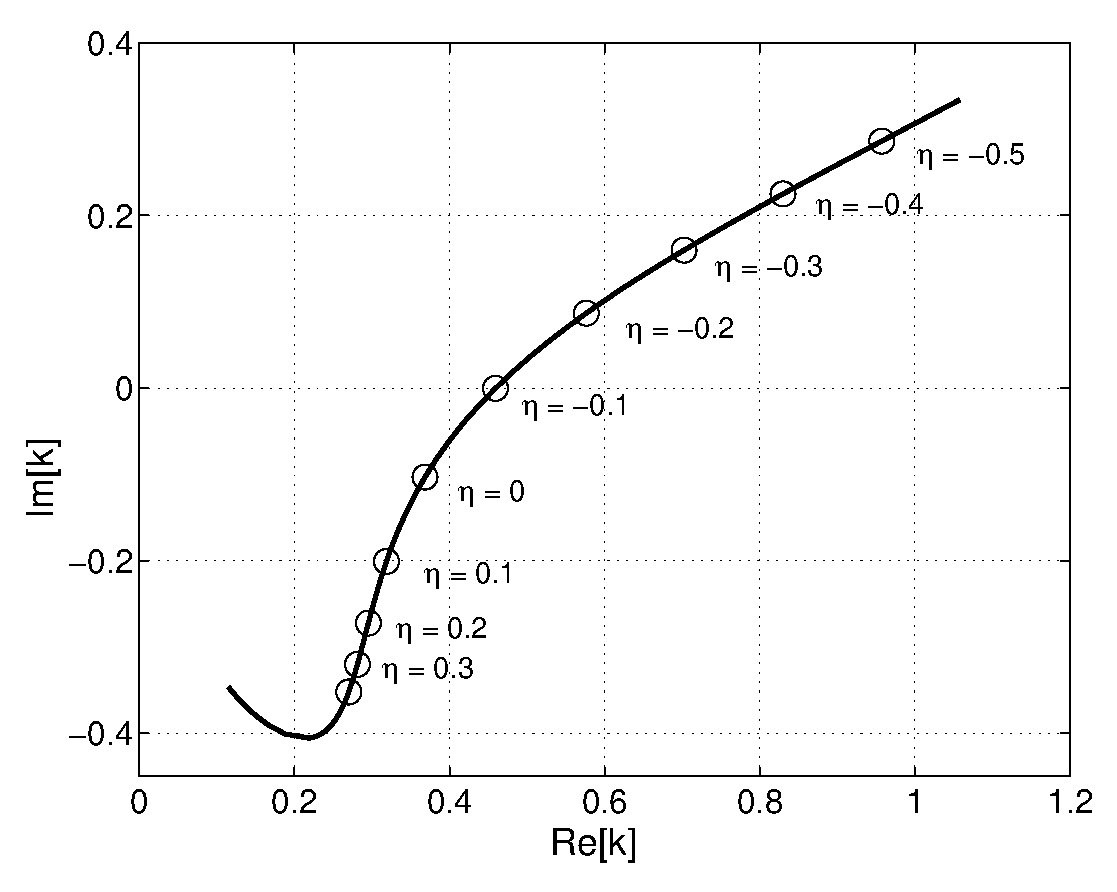
\epsfig{file=figures/optical2.eps}}
\end{center}
\caption{Pole trajectory of the $l=1$ resonance in the $\nu_A = -5$ Malfliet-Tjon interaction,
for increasing absorbtion/emission. Here both attractive and repulsive strengths of the interaction
takes complex values,$ V  \rightarrow (1+\eta i)V$ .}
\label{fig:optical2}
\end{figure}
In scaling both the attractive and repulsive parts of the potential with the 
same complex constant $ 1 + \eta i $, both absorbtion and emission takes place.
However, since the potential is on average more attractive than repulsive, the 
total effect of letting $ \eta $�become negative will be emission of particles
while letting $ \eta  $ become positive will result in absorbtion of particles. This is 
also seen from the figure~\ref{fig:optical2}, where the pole moves towards the
physical sheet for $�\eta < 0$, and becomes more ``unphysical'' for $ \eta > 0$.  
Since absorbtion and emission are competing processes in this case, the dependence
of the pole position on increasing/decreasing imaginary part of 
the potential should be weaker than in the 
former case where only the attractive part was scaled, i.e.  pure 
absorbtion and emission took place. 
This is observed from figures.~\ref{fig:optical1},\ref{fig:optical2}. In figure~\ref{fig:optical1}
the pole has moved onto the physical energy sheet for $ \eta = - 0.1 $ while
it is still on the nonphysical sheet in figure~\ref{fig:optical2}. The same strong and weak 
dependence on $\eta $ is observed for the absorbtive process $ \eta = 0.1 $. � 

For comparison with the results for the Malfliet-Tjon potential above, 
the pole trajectory for  the $l=1$ 
Yamaguchi interaction with $\beta = 2 \:\mathrm{fm}^{-1}$ and 
interaction strength $ \lambda = 165 \:\mathrm{MeVfm}^{-1} $ is considered as well
\footnote{See Paper I for details on the $l=1$ Yamaguchi potential}. 
This interaction supports a resonance at $ E = 0.8736 -0.1285i $ MeV 
for $\eta = 0 $. Figure~\ref{fig:optical3} gives a plot of the pole trajectory 
of the resonance for varying $\eta $. 
\begin{figure}[hbtp]
\begin{center}
\resizebox{9cm}{7cm}{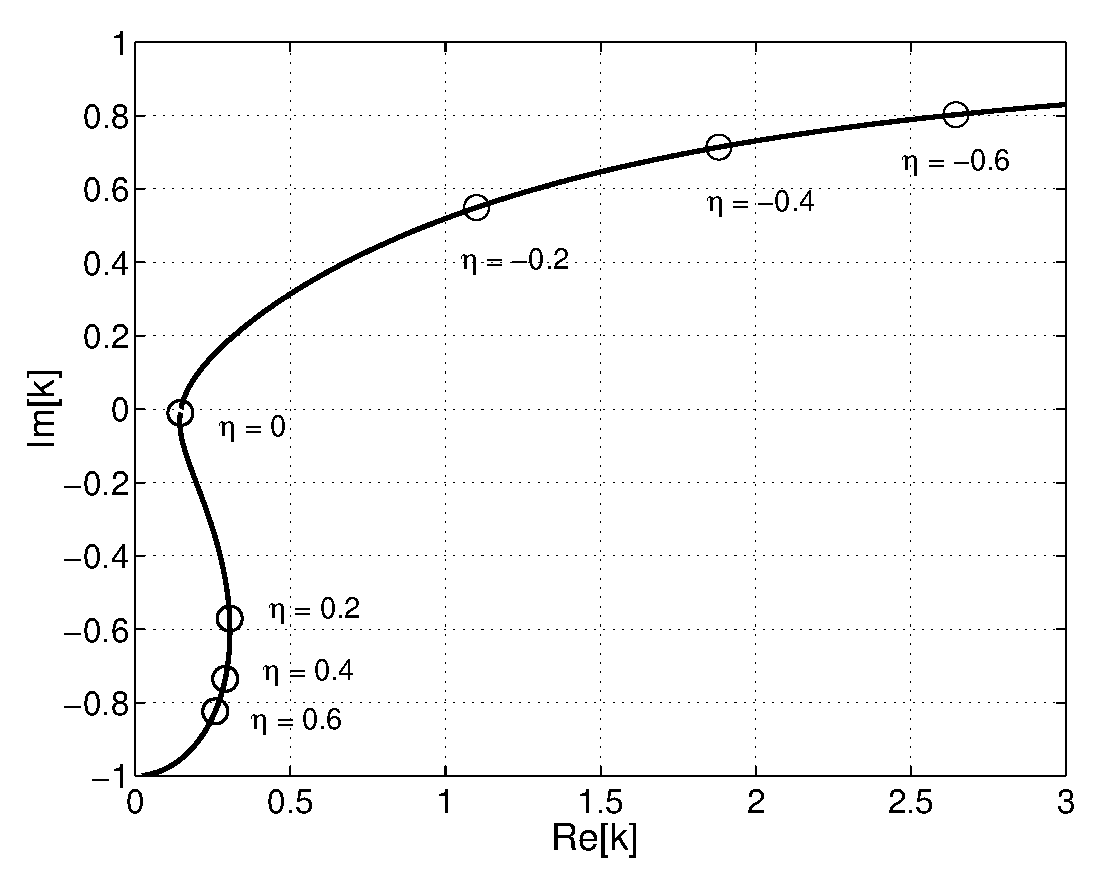
\epsfig{file=figures/optical3.eps}}
\end{center}
\caption{Pole trajectory of the resonance at 
 $ E = 0.8736 -0.1285i $ MeV  in the Yamaguchi interaction with 
$\beta = 2 \:\mathrm{fm}^{-1}$ and 
 interaction strength $ \lambda = 165 \:\mathrm{MeVfm}^{-1} $ }
\label{fig:optical3}
\end{figure}
From the figure it is seen that pole behaves in the same way with increasing 
emission  and  absorbtion as in the Malfliet-Tjon case considered in figures~\ref{fig:optical1} and 
\ref{fig:optical2}.

From the  above numerical analysis of the resonance pole trajectory for 
a complex absorbing or emitting potential, one may make the following conclusion.
For increasing emission, i.e. $ \eta < 0 $,  the resonant pole 
in the third quadrant of the complex $k$-plane
moves towards the real $k$-axis.
Eventually the resonant poles move
through the unitarity cut and 
onto the physical energy sheet (upper half complex $k$-plane). 
When the pole crosses the cut, the imaginary part of the resonance energy is 
zero, that is why poles located on the cut are usually defined as 
\emph{bound states embedded in the continuum}. 
Poles which are located on the physical energy sheet 
may be interpreted as unstable bound states. 
Poles moving onto the physical energy sheet may therefore give a clear 
signature in physical observables such as phaseshifts and scattering cross sections.
For increasing absorbtion on the other hand, i.e. $\eta > 0$ , the resonant pole 
becomes more and more unphysical in the sense that it moves away from the
physical scattering axis. These conclusion apply in all cases considered above,
and one may expect these conclusions to hold for other potential shapes. 

The illustrations above indicates a general behaviour of decay resonant states 
when the interaction is scaled by a complex constant. One may ask in a similar fashion 
in what way the capture resonant states develops as a function of $\eta$. Will the symmetry 
with respect to the imaginary $k$-axis for capture and decay states prevail ? 	
The answer to this is no. It can be seen by considering the symmetry properties of the 
scattering matrix in the case of a complex interaction. In particular we have the 
property, see equations~(\ref{eq:sym1},\ref{eq:sym2}) 
\begin{equation}
S_l^*(-k^*,\eta^*)  = S_l(k,\eta) 
\end{equation}
This implies that if the interaction $ (1+i\eta )V$ supports a 
resonance at $k$, the complex conjugated interaction $ (1+i\eta)^*V$ supports a resonance at
$ -k^*$. The number of poles is invariant with respect to $\eta $, the poles
only get redistributed as $\eta$ is varied. The symmetry between decay and capture states
is therefore broken. As the capture resonance moves away from the real $k$-axis in the third
quadrant of the complex $k$-plane the capture state moves toward the real $k$-axis and 
eventually into the physical energy sheet. It is quite interesting that a capture state
which for $\eta = 0 $ was considered a non-physical state, may become a physical bound state
with a finite lifetime for $\eta > 0$.  
\begin{figure}[hbtp]
\begin{center}
\resizebox{9cm}{7cm}{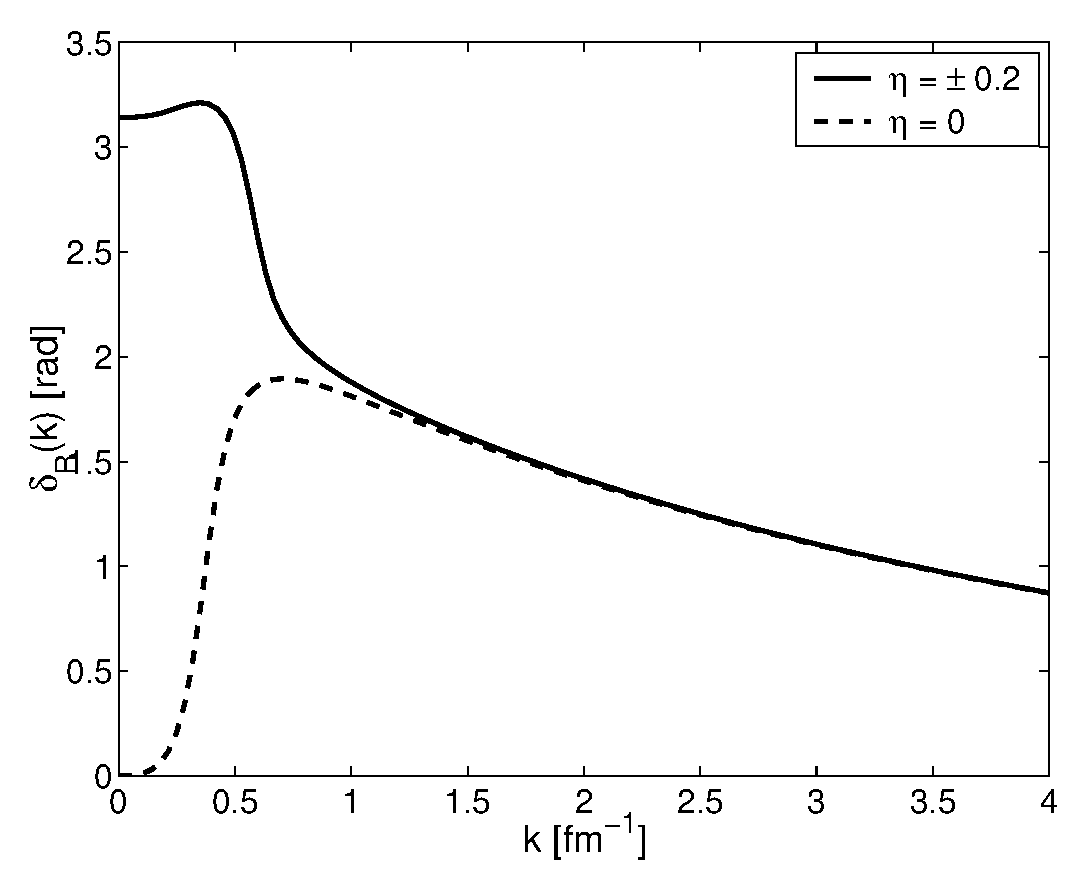
\epsfig{file=figures/mt_phase_opt.eps}}
\end{center}
\caption{Real part of phase shifts for the $l=1$ Malfliet-Tjon interaction with
$ \nu _A = -5$. The dashed line gives the phase shifts for $\eta = 0 $,
while the continuous line give the phase shifts for $ \eta \pm 0.2 $.}
\label{fig:mt_phase_opt}
\end{figure}

\begin{figure}[hbtp]
\begin{center}
\resizebox{9cm}{7cm}{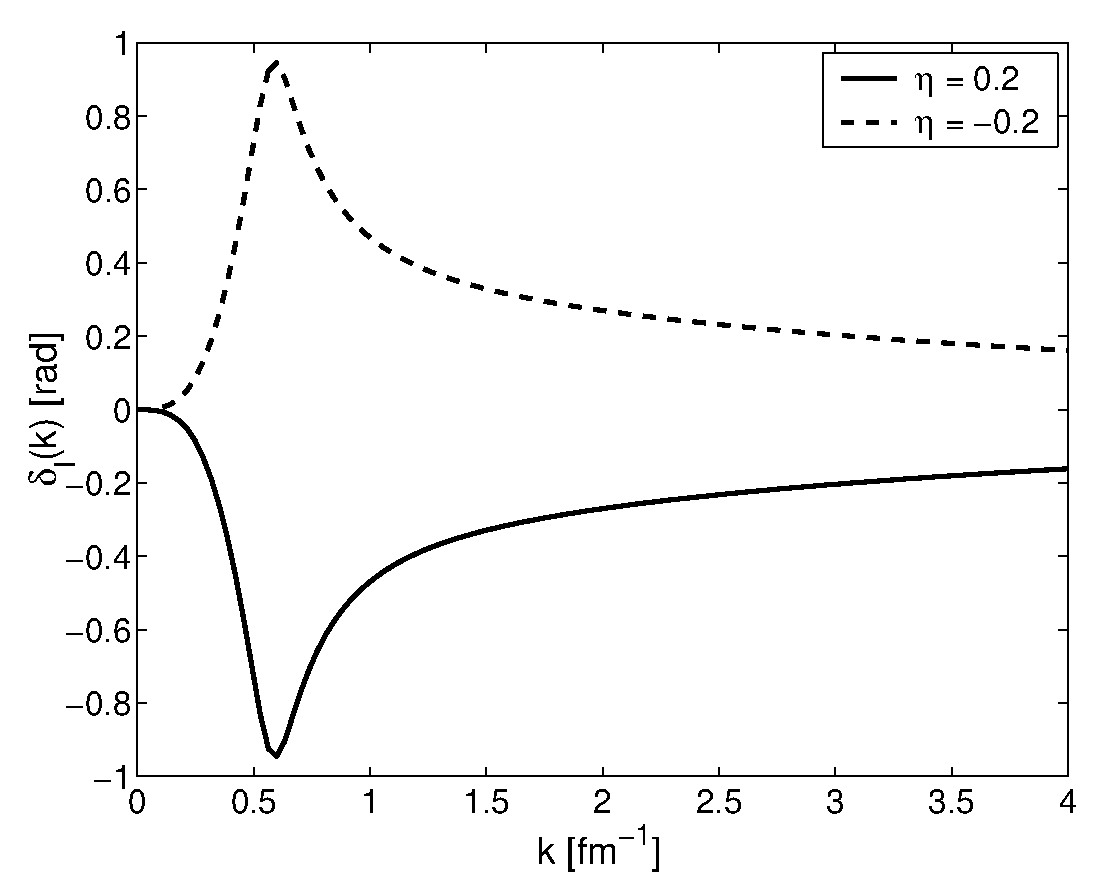
\epsfig{file=figures/mt_phase_opt2.eps}}
\end{center}
\caption{Imaginary part of the phase shifts for the $l=1$ Malfliet-Tjon interaction with
$ \nu _A = -5$ and $\eta = -0.2 $ given by the dashed line and $ \eta = 0.2 $ by the continuous line.}
\label{fig:mt_phase_opt2}
\end{figure}


In the case of complex interactions the phase shift is a complex quantity, $\delta = \delta_R + i \delta_I$, 
the real part $\delta_R$ is interpreted as before and describes the elastic scattering while
the imaginary part, $\delta_I $,  is a measure of the inelastic scattering taking place. 
Figures~\ref{fig:mt_phase_opt},\ref{fig:mt_phase_opt2} 
gives a plot of the real and imaginary part of the phase shifts for  
the $l=1$ Malfliet-Tjon interaction with
$ \nu _A = -5$ and $\eta = 0, \pm 0.2 $. Here only the attractive strength $V_A$ 
was scaled, keeping the
repulsive part $V_R$
real, see figure~\ref{fig:optical1} for details on the pole trajectory.
In the case $ \eta = -0.2 $ the decay state
has moved onto the physical energy sheet and become a bound state. In the case 
$ \eta = 0.2 $ the capture state has moved into the physical energy sheet and become a bound state, 
while the decay state has become more unphysical.
There is no way to differentiate between the real part of the phase shifts for $\eta = \pm 0.2 $.
The elastic scattering is the same for both cases, which is expected since the real part of the
interaction is the same. The imaginary part of the phase shifts are on the other hand different, and
is directly related to the sign of $\eta $ where either an absorbtion of particles out of
the elastic channel or an emission of particles into the elastic channel takes place. 

A generalized Levinson theorem may be formulated for the real part of the phase shift \cite{kukulin}, 
$\delta_R(0) -\delta_R (\infty ) = n\pi $ 
where $n $ is the number of poles in the upper half complex $k$-plane (physical energy sheet). 
In figure.~\ref{fig:mt_phase_opt}
we have for $\eta = \pm 0.2 $ , $\delta (0) = \pi $ which is in accordance with the generalized
Levinson' theorem. 

% new section
\section{Two-particle scattering; isolating resonance phenomena by CDM}
In this section we will discuss the solution for the full
off-shell $t$-matrix, and hence the full two-body scattering problem, by expanding 
the two-body Green's function in a complete set of Berggren states. 
The Berggren representation of the scattering equations gives 
an analytic continuation in energy, from the upper rim of
cut through the cut and into the non-physical energy sheet.     

The $t$-matrix is defined in operator form by 
\begin{equation}
\label{eq:t1}
t(\omega)  = V + Vg^{II}(\omega)V,
\end{equation}
or 
\begin{equation}
\label{eq:t2}
t(\omega) =  V + Vg_0^{II}(\omega)t(\omega).
\end{equation} 
Here $\omega$ is the incoming energy, $ g^{II}(\omega) $ is the resolvent, 
commonly known as the Green's operator, and $g_0^{II}(\omega) $ the 
corresponding free Green's operator. In operator form they are defined by
\begin{eqnarray}
  g_0^{II}(\omega) & = & {1\over \omega - H_{0}}, \\ 
  \label{eq:greensfunc}
  g^{II}(\omega) & = & {1\over \omega - H }. 
\end{eqnarray}
They are related through the Dyson equation
\begin{equation}
  g^{II}(\omega) = g_0^{II}(\omega) + g_0^{II}(\omega)Vg^{II}(\omega)
\end{equation} 
The term $H_{0}$ is the kinetic energy operator and $H$ the full two-body
Hamiltonian. The physical interpretation of the Green's functions is that $g_0^{II} $ 
describes the propagation of two noninteracting particles, and $g^{II}$ 
describes the propagation of two interacting particles in free space.

\subsection{Berggren representation of the $t$-matrix}
The Berggren representation of the Green's function is obtained by expanding the unit 
operator using the completeness relation given in equation~(\ref{eq:unity2}). In this case 
the Green's operator takes the form
\begin{equation} 
 \label{eq:spectral2}
g^{II}(\omega) = \sum _{n = a,b,c,d} {\vert\psi _{n}\rangle\langle \psi^* _{n}\vert\over 
\omega - E_{n}} + \int _{L^+} dE{\vert\psi\rangle
\langle\psi^*\vert\over \omega - E}.
\end{equation}	
Here $n$ denotes bound, antibound and resonant states. The integration contour $L^{+}$
denotes an arbitrary inversion symmetric contour, see e.g. figure~\ref{fig:int_contour2}  in 
SubSec.~\ref{sec:berggren} of Chapter~\ref{chap:gentheory}, 
and gives the non-resonant distorted continuum contribution to   
the interacting Green's function. If we neglect the non-resonant continuum contribution 
to the Green's function we get the \emph{resonant state expansion} of the Green's  
function. Such expansions have been studied over the last decade for finite range potentials, 
see e.g. \cite{vertse, vertse1, lind}. The Green's function given in equation~(\ref{eq:spectral2})     
is continuous and analytic in energy across the real axis and into the domain ${\bf C} $ of 
the lower part of the complex energy plane. Equation ~(\ref{eq:spectral2}) is therefore an analytic 
continuation in energy of the Green's function defined along the real energy axis. 

The Berggren representation of the $t$-matrix is obtained by inserting the 
interacting Green's function given by equation~(\ref{eq:spectral2}) into equation~(\ref{eq:t1}), giving
\begin{equation}
t(\omega) = V + \Delta t(\omega) = V + \Delta t^{R}(\omega ) + \Delta t^{C}(\omega).
\end{equation}
Here $\Delta t^{R}(\omega )$ is the resonant contribution while
$ \Delta t^{C}(\omega) $ is the non-resonant distorted continuum contribution to 
the $t$-matrix.
By projecting $t(\omega)$ on momentum states, and decomposing
into partial waves, the  $t$-matrix elements $t_{l}(k,k';\omega) $ can be 
expressed as 1-dimensional integral equations,
\begin{equation}
\nonumber
t_{l}(k,k',\omega) = V_{l}(k,k')  
\label{eq:tmat2}
 + \int _{L^{+}}\int _{L^{+}} dq\:d{q'}
\: q^{2}{q'}^{2}
V _{l}(k,q)g^{II}(q,q';\omega)V_{l}(q',k'), 
\label{eq:tmat1}
\end{equation}
This representation of the $t$-matrix is valid as long as we do not pass
through any singularities of the interaction potential by deforming the real 
$k$-axis into the distorted contour $L^{+}$. 

In numerically solving for equation~(\ref{eq:tmat1}), the eigenvalue 
problem on the discretized contour $L^+$ given in equation~(\ref{eq:momentum_space3}) has to be solved.
Then the interacting Green's function is represented in the discretized 
complete set of momentum states given in equation~(\ref{eq:unity2}), giving the discretized
Green's function, 
\begin{equation}
  g^{II}(k_i,k_j, \omega) = \sum _{n}{\psi_{nl}(k_i)\psi_{n l}(k_j)\over  \omega - E_{nl}} = 
  \sum _{n}\left( \sqrt{w_iw_j}k_ik_j\right)^{-1}{\psi_{nl}(i)\psi_{n l}(j)\over  \omega - E_{nl}}.
\end{equation}
Inserting this discretized form of the interacting Green's function into 
equation~(\ref{eq:tmat1}) and discretizing the integration over $q$ and $q'$, 
a discretized version of the $t$-matrix is obtained. Having obtained $g^{II}(k_i,k_j) $,�
the full off-shell $t$-matrix is therefore obtained by the matrix equation
\begin{equation}
  t_l(k_i,k_j,\omega) = V_l(k_i,k_j) + \tilde{V}_l^T(i) \tilde{g}^{II}(\omega ) \tilde{V}_l(j) 
\end{equation} 
where $\tilde{V}_l(n)$ is the $n$'th column of the potential matrix $V_l(k_i,k_j)$ 
and $\tilde{g}^{II}(\omega)$is the matrix
\begin{equation}
  \tilde{g}^{II}(i,j,\omega) = \sqrt{w_i w_j}k_ik_j 
  \sum _{n}{\psi_{nl}(i)\psi_{n l}(j)\over  \omega - E_{nl}}.
\end{equation}
Applying CDM enables us to 
obtain $t_{l}(k,k';\omega) $ for both real and complex energies $\omega�$. 
The integral becomes non-singular on the deformed contour for real and positive 
input energies $\omega $, resulting in numerically stable solutions for physical
two-body scattering. Equation~(\ref{eq:tmat1}) can also be considered as an
analytic continuation of equation~(\ref{eq:tmat1}) for complex input energies $\omega$,
and stable numerical solutions can be obtained for complex energies above the 
distorted contour. The Berggren representation of the $t$-matrix also allows for a
separate study of the resonant and continuum contributions.   
The limitation of this method is due to that most  potentials
in momentum space have singularities in the complex plane when one argument 
is real and the other is complex.
By applying contour $L_{1}^{+}$, which is based
on rotation into the complex plane, in most cases there will be restrictions
on both rotation angle ($\theta$) and maximum  incoming and outgoing momentum 
($k,k'$), see for example Ref.~\cite{nuttal}. 

Using contour $L_{2}^{+} $ we can avoid these limitations by 
choosing the integration contour in such a way that the potential 
singularities always will lie outside the integration contour, and therefore
do not give any restriction on rotation angle and maximum incoming and outgoing
momentum.

\subsection{Fredholm representation}
The partial wave decomposition of equation~(\ref{eq:t2}) gives the \emph{Fredholm} 
representation, commonly known as the Lippmann-Schwinger equation  
\begin{equation}
\label{eq:tmat3}
t_{l}(k,k';\omega) = V_{l}(k,k')+
{2\over \pi}\int _{0}^{\infty } {dq q^{2}V_{l}(k,q)t_{l}(q,k')\over \omega - E(q) }.
\end{equation}
In physical two-body scattering the input energy is real and positive. In this
case the \emph{Fredholm} integral equation~(\ref{eq:tmat3}) has a singular
kernel of Cauchy type. Solving singular integrals can be done 
by Cauchy's Residue theorem, where we 
integrate over a closed contour enclosing the poles. There are two ways of
doing this, either by letting $ z $ lie an infinitesimal distance above the 
real axis, i.e., $ \omega \rightarrow z + i\epsilon $,  or by letting $ \omega�$
lie on the real axis. In both cases we must choose a suitable contour enclosing the
 singularity. If we choose the latter position of the singularity,  we get  
 a  Cauchy \emph{principal-value} integral where we integrate up to - but not
 through - the singularity, and a second contour integral,  where the 
contour can be chosen as a semicircle around the singularity. 
Equation~(\ref{eq:tmat3}) can thus be given in terms of a principal value part and a 
second term coming from integration over the semicircle around the pole. The result is
\begin{equation}
\label{eq:pv1}
 t_{l}(k,k';\omega)  = V_{l}(k,k') + {2\over \pi}
\mathcal{P}\int _{0}^{\infty } {dq q^{2}V _{l}(k,q)t_{l}(q,k')\over \omega - E (q) } 
 \:- \: 2i\mu k_{0}V_{l}(k,k_{0})t_{l}(k_{0},k';\omega).
\end{equation}
By rewriting the principal value integral using the relation
\begin{equation}
\mathcal{P}\int_{0}^{\infty}dk\: {f(k)\over k_{0}^{2} - k^{2}} =  
\int_{0}^{\infty}dk\: {[f(k)-f(k_{0})]\over k_{0}^{2} - k^{2}}, 
\end{equation}
we obtain an equation suitable for numerical evaluation.
Equation~(\ref{eq:pv1}) can be converted into a set of linear 
equations by approximating the integral by a sum over $N$ 
Gaussian quadrature points $( k_{j}; j = 1,...N  ) $, each weighted by $ w_{j} $ 
The full off-shell $t$-matrix is then obtained by matrix inversion. This
method for solving integral equations is known as the Nystrom method. 
It is numerically effective and stable, except for the rare case when
 the incoming energy $\omega$ coincides with or is very close to one of the 
integration points. 

So far we have only considered physical input energies in 
equation~(\ref{eq:tmat3}), but it has been shown in Ref.~\cite{kukulin} 
that the analytically 
continued Lippmann-Schwinger equation to complex energies takes the same form
as equation~(\ref{eq:pv1}). By solving the full off-shell $t$-matrix for arbitrary 
complex input energy, we do not have to alter the set of linear equations
obtained for physical energy, the only modification is that the energy is
complex. 

The Lippmann-Schwinger equation  for $t$-matrix (\ref{eq:tmat3}), 
can be solved by the contour deformation method as well. Using CDM the integral equation
given in equation~(\ref{eq:tmat3}) has a compact integral
kernel (Schmidt kernel) 
for positive incoming energies $\omega$, 
thus the principal value (PV) prescription may be avoided. 
In the first step we calculate the $t$-matrix elements $t_l(z,k,\omega)$ 
where $k$ is on the real axis and $z$ is on a suitable deformed contour $L^+$.
This is obtained by solving the integral equation, 
\begin{equation}
  \label{eq:tmat4}
  t_{l}(z,k;\omega) = V_{l}(z,k)+
  \int_{L^+} {dz' {z'}^{2}V_{l}(z,z')t_{l}(z',k)\over \omega - E(z') }.
\end{equation}
Here it is seen that for real input energies $\omega $ 
the integral kernel is non-singular sincel the kinetic energy term $E(z)$ is
defined on a deformed contour in the complex $k$-plane. Having obtained 
$t_l(z,k;\omega) $ the $t$-matrix elements $t_l(k,k';\omega)�$ is 
straightforward obtainable by the non-singular integral, 
\begin{equation}
  \label{eq:tmat5}
  t_{l}(k,k';\omega) = V_{l}(k,k')+
  \int_{L^+} {dz {z}^{2}V_{l}(k,z)t_{l}(z,k')\over \omega - E(z) }.
\end{equation}
here $k$ and $k'$ are given along the real $k$-axis, while $z$�
is 
defined along the deformed integration contour $L^+$.
This two-step procedure using CDM offers an alternative approach to the numerical
solutions for the $t$-matrix. Stable solutions will be obtainable as long 
as the contour does not pass through any singularities of the potential.
Below we consider the solution of the $t$-matrix for the Malfliet-Tjon potential 
by CDM and compare results with the standard principal value (PV) prescription.
First of all, we have to determine the singularity structure of the potential 
Malfliet-Tjon potential. From equations~(\ref{eq:tmat4},\ref{eq:tmat2}) it is seen that the potential 
must be defined for one real variable $k$ and 
one complex variable $z$ given on the contour $L^+$. 
So in conclusion, the contour $L^+$ must be chosen in such a way that the 
potential admit analytical continuation from the real $k$-axis to the 
complex contour $L^+$. 

For an illustration we  consider two contours $C_1$ and $C_2$.
The $C_1$ contour is just the phase transformation, or complex rotation, 
$ C_1 \: : \:\:�\vert k \vert exp(-i\theta) $. The $C_2$ contour consits of a combination of 
a rotation and a translation in the complex $k$-plane\footnote{See Paper I for further details. 
In this particular study
natural units are used, i.e. the momentum $k$ is in units of MeV and the potential 
is in units of MeV$^{-2}$. In Paper I conventional units were used.}.  
If we integrate along contour $C_{1} $ there will always be a singularity on the 
contour given by 
\begin{equation}
z = k_{\mathrm{max}} - i\mu,
\end{equation}
where
\begin{equation}
k_{\mathrm{max}} = \mu /\tan(\theta ),
\end{equation}
and $\mu = \mathrm{min}[\mu_{A},\mu_{B}] $\footnote{$\mu $ is here considered as the mass  
of the pions entering the Yukawa potentials; $V(r) = V_0exp(-\mu r)/r$}. 
For $k,k' > k_{\mathrm{max}}�$ the contour $C_{1}$ will 
pass through the singularity of the interaction. 
However, if the interaction, $V_{l}(k,k') $, is approximately zero for $k,k' > k_{\mathrm{max}} $,
or the $t$-matrix is wanted only in the low momentum regime ($ k,k' \ll  k_{\mathrm{max}} $),
integrating along contour $C_{1} $ can be done as long as 
\begin{equation}
\theta < \arctan \left( \mu/ k_{\mathrm{max}} \right ).
\end{equation}
In this sense we may call $k_{\mathrm{max}} $ the cutoff momentum. 
This choice may cause numerical unstable solutions for small values of momenta, 
since the rotated contour may lie very close to the real $k$-axis where the
integral kernel is singular.  
The same conclusion has already been pointed out by Nuttal in Ref.~\cite{nuttal2}.

Here we see the advantage of integrating along contour $C_{2}$. Not only 
will it be able to reproduce virtual states (see Paper I), but it yields also
accurate results for  the $t$-matrix for real incoming and outgoing momenta.
It will always  be possible to choose a contour $C_{2}$ lying above the nearest singularity $z = \Re[k] - 
i\mu $, implying no restriction on rotation angle $\theta $ irrespective of cutoff 
momentum $k_{\mathrm{max}} $. Figure~\ref{fig:newfig8} gives an illustration. 
\begin{figure}[hbtp]
\begin{center}
\resizebox{9cm}{7cm}{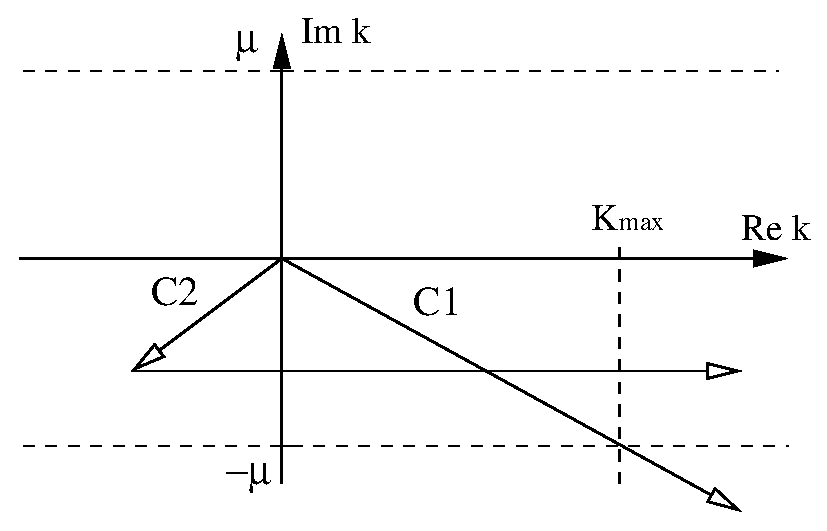
\epsfig{file=figures/newfig9.eps}}
\end{center}
\caption{Illustration of potential singularities for the Malfliet-Tjon interaction $V_{l}(k,z)$, 
where $k$ is real  and $z$ complex. Restriction on the integration contours $C_{1} $ 
and $C_{2}$
is clearly seen for given cutoff momentum $k_{max�} $ ($V_{l}(k,k') \approx 0 $ for 
$k,k' > k_{\mathrm{max}} $). }
\label{fig:newfig8}
\end{figure}

Figure~\ref{fig:newfig9} shows a plot of the calculated $t$-matrix elements
$t_{l}(k,k;E) $ for incoming energy $E = 100$ MeV for the $s$�-wave Malfliet-Tjon
interaction, using the contours $C_{1} $ and $C_{2}$. In this case we used a 
rotation angle $\theta = \pi/6 $ for both contours, and a translation $b = 
300$ MeV for contour $C_{2}$. The Malfliet-Tjon interaction has a 
singularity along contour $C_{1}$, given by $k_{\mathrm{max}} = \mu /\tan(\theta ) = 
529.77$ MeV. In this case the interaction 
is not sufficiently neglible for $k,k' > k_{\mathrm{max}}$,
and using contour $C_{1}$ will not give accurate calculation of the $t$-matrix. 
\begin{figure}[hbtp]
\begin{center}
\resizebox{9cm}{7cm}{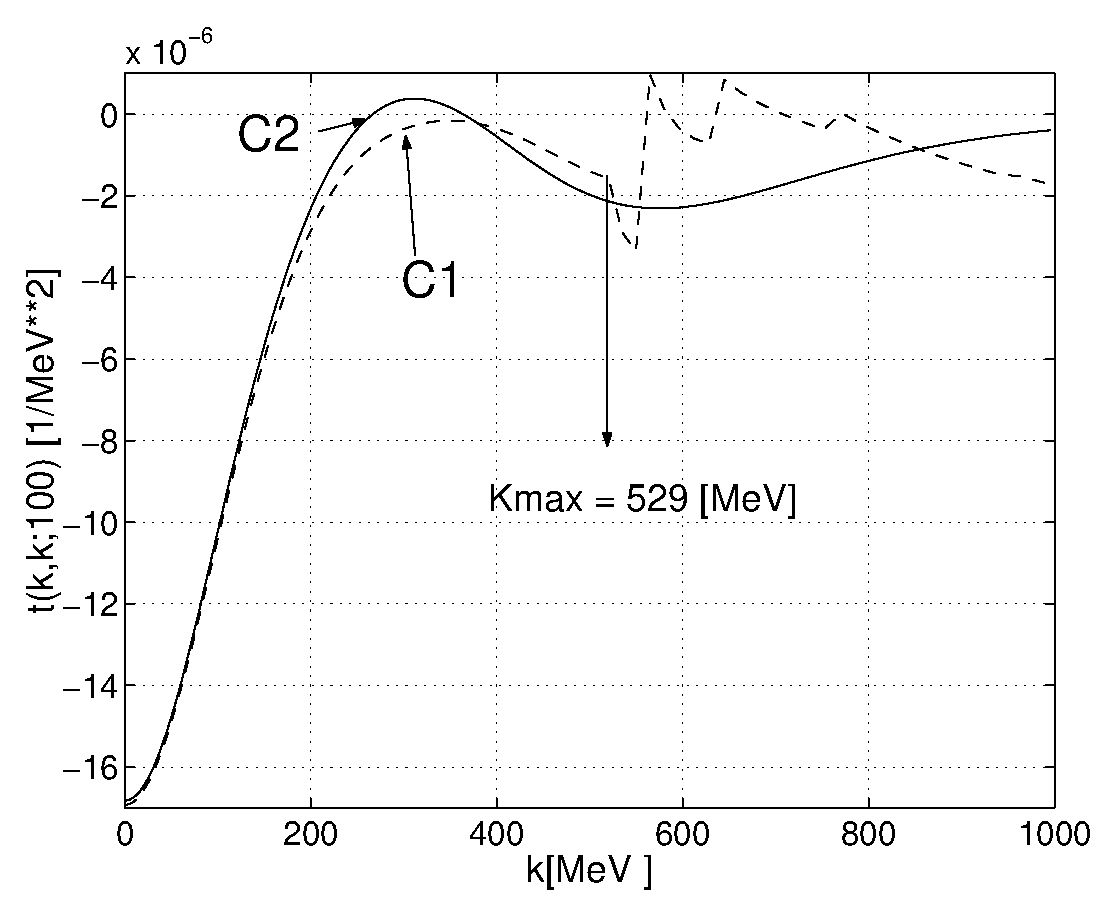
\epsfig{file=figures/newfig10.eps}}
\end{center}                                           
\caption{Plot of $t$-matrix elements for the $s$-wave Malfliet-Tjon interaction
using the contour $C_{1}$ (dashed line) and the contour $C_{2}$ (solid line).
The potential singularity along contour $C_{1}$ is clearly displayed, and
located at $k_{\mathrm{max}} = 529.77$ MeV.}
\label{fig:newfig9}
\end{figure}
This illustrates clearly the advantage of integrating along the contour $C_{2}$
instead of $C_{1}$, and the importance of choosing a contour which avoids
singularities in the potential. 

For a comparison of CDM with the standard PV prescription in
solving for the $t$-matrix numerically we consider the 
the on-shell unitarity for the $S$-matrix calculated with both methods. 
Table~\ref{tab:tab7} reports
calculations done by the principal value prescription and the
contour deformation method $C_{2}$. The calculations used $N=50 $ 
integration points for the principal value
integration, for the contour deformation method we used $30$ points
along the rotated line and $N_T = 
100,200$ along the translated line.  
We observe that we need a higher number of integration points
along the translated line of $C_{2}$ in order to obtain a comparable accuracy with
the PV method.
\begin{table}[htbp]
  \begin{tabular}{rrrrr}
\hline
    \multicolumn{1}{c}{} & \multicolumn{1}{c}{PV} & \multicolumn{2}{c}{CDM} \\
\hline
    \multicolumn{1}{c}{$k$[MeV]} & \multicolumn{1}{c}{$N = 50$} & \multicolumn{1}{c}{$N_T = 100 $} &
    \multicolumn{1}{c}{$N_T = 200 $ }  \\
    \hline
    10. & 	1.00000000 & 	 1.00000811 & 	1.00000811 \\
    110. & 1.00000000 & 	 0.999999940 &	 1.00000000 \\
    210. & 1.00000000 & 	 0.999999940 &  1.00000000 \\
    310. & 1.00000000 &	0.999999881 &	1.00000000 \\
    410. & 1.00000000 &	 0.999999881 &	1.00000000 \\
    510. & 1.00000000 &	 0.999999881 & 	1.00000000 \\
    610. & 1.00000000 &	0.999999881 & 	1.00000000 \\
    710. & 1.00000000 & 	 0.999999821 &	1.00000000 \\
    810. & 1.00000000 & 	0.999999821 &	1.00000000 \\
    910. & 1.00000000 &	0.999999821 &	1.00000000 \\
    1010.& 1.00000000 &	0.999999762 &	1.00000000 \\
    1110.&  1.00000000& 	 0.999999702 &	 1.00000000 \\
    1210.&  1.00000000& 	 0.999999702 & 	1.00000000 \\
    1310.&  1.00000000& 	 0.999999642 & 	1.00000000 \\
    1410.&  1.00000000& 	 0.999999523 & 1.00000000 \\
    1510.&  1.00000000& 	 0.999999642 & 	1.00000000 \\
    \hline
  \end{tabular}
  \caption{Calculations of $S$-matrix norm, $\vert S(k) \vert $, for the $s$-wave
    Malfliet-Tjon potential with parameters  $ V_{A} = 7.291$ MeV, 
    $\mu_{A} = 613.69$ MeV, $V_{B} = -5$ MeV and  $\mu_{B} = 305.86$ MeV. Column 2 gives results for the
    principal value prescription (PV), while columns 3,4 give results for the contour
    deformation method (CDM).}
\label{tab:tab7}
\end{table}


% new section
\section{Application of CDM to resonance-like phenomena in nuclear matter;
  pair instabilities and the onset of pairing}
\subsection{2p2h spectral structures in a nuclear medium.} 
\label{sec:inmedium}
In this section we discuss the application of CDM to nucleon-nucleon scattering
in infininte nuclear matter. Of particular interest is the formation and decay of
two nucleon bound- and resonant states in nuclear matter. In the early 70's 
Bishop \emph{et. al.} ~\cite{bishop1,bishop2} showed that the existence of bound state
pairs in a nuclear medium can be directly linked to the singularities of the 
in-medium t-matrix. 
The existence of bound pair states in nuclear medium, 
is closely related to the concept of \emph{cooper} pairs. Cooper pairs are
considered as the formation of bound electron pairs in a degenerate electron gas,  
giving rise the phenomenon of \emph{super conductivity}.
Treating holes on equal footing with particles  Bishop \emph{et. al.} 
showed that the pairing effects in nuclear matter 
where increased when comparing with
the standard Bethe-Goldstone approach where only particle propagation 
is considered, see e.g. Ref.~\cite{haftel}. 
In Ref.~\cite{goldberg} showed that the BCS gap equation is directly related 
to the 2p2h bound pair states. Two decades later Dickhoff \emph{et. al.} \cite{dick1,dick2,dick3}
discussed similar properties of composite pair states in nuclear matter,
and formally related the BCS gap equation to the
2p2h self-consistent eigenvalue equation for the bound states.
There it was suggested that strong pairing effects would be present
in nuclear matter
at certain densities and total momentum, due to the existence of bound pair states.

It is well known that for a realistic nucleon-nucleon interaction there may appear 
pairing instabilities in attractive partial waves near the fermi surface. 
For a continuous single particle spectrum pairing instabilty is 
interpreted as an instability to form bound 2p2h states in nuclear matter.  
These pairing instabilities appear as complex poles located around the fermi surface 
in the effective interaction $\Gamma $. In determining the self consistent self energy, 
one should take the complete energy dependence of the effective interaction into account. 
In earlier calculations only the non-resonant continuum portions of the effective interaction
were taken into account. The inclusion of $K = 0$ 2p2h bound states in the 
calculation of the self energy, was discussed in Ref. (). 

For a continuous single particle spectrum these 2p2h bound 
pair states appear as complex  poles of the effective interaction, 
located around the Fermi energy $2e_f$. 
These singularities give rise to serious numerical 
problems when solving the iterated Feynman - Galitskii integral equation for the 
effective interaction. In Ref.~\cite{dick3} it was proposed that an introduction of a gap in 
the single particle spectrum located at the fermi surface would resolve this problem.  
This suggestion was based on the observation that the 2p2h bound state poles 
become real poles by introducing a gap in the single particle spectrum at the fermi surface. 
If there is no gap in the single particle energy spectrum, there
is no room for the bound states to appear as real excitations, since the hole-hole continuum 
extends from $-\infty $ to $ 2e_f$�and the particle-particle continuum extends from 
$2e_f$ to $\infty$. So the $2p$ and $2h$�poles appear at complex conjugate energies, 
$E_{2p} = E_{2h}^*$, around the Fermi energy $2e_f$, this is why the poles of the $t$-matrix
are often called pair-instabilities. By introduction of a mininum gap in the single particle 
spectrum this instability will disappear and the poles will position themselves on the
real energy axis between $2e_f^+ $ and $ 2e_f^-$.
Ultimately this gap at the fermi surface would be generated self consistently. 

The 2p2h bound states are dependent on both the fermi momentum $k_f$ and the total momentum 
between the nucleons $K$. 
The 2p2h bound states appear only in a specific density 
region where strong pair correlations are expected, and will eventually dissolve with increasing
center of momentum (total momentum) between the nucleons. 
In this case the complete energy spectrum is exposed without analytic continuation of the eigenvalue 
problem into the complex $k$-plane. However, 
with increasing $K_{CM}$ the 2p2h poles will move towards  
2p2h continuum, and one may expect that the 2p2h poles will move into the lower half 
$k$-plane (non-physical energy sheet) 
for a center of momentum $K$ greater that some critical value $K_{max}$. 
In close analogy with the free scattering case, these poles may be associated with 
either virtual or resonant states. In this case CDM may prove to be a 
reliable and efficient way to calculate these exotic 2p2h states. 
These 2p2h poles will also appear as singularities in the effective interaction, and may
on the same level as the bound state poles cause numerical trouble. 
One may expect that an introduction of a gap at the fermi surface will 
not make these complex poles real poles, since they are located on the non-physical energy sheet.
From this observation one may conclude that
an introduction of a gap at the fermi surface does not completely solve the problem 
associated with pairing instabilities in the iterated effective interaction $\Gamma $. 

We start by outlining the formalism for 2p2h  
bound and scattering problems in infinite nuclear matter, and 
emphasize the relation  between the $t$-matrix and the
two-nucleon eigenvalue equation in nuclear matter.
Holes and particles are treated on equal footing, 
hence allowing for hole-hole and particle-particle propagation. 
Solving for the effective interaction, $\Gamma $,
the particle - particle and hole - hole ladder diagrams are summed to infinite order.
The influence of the surrounding medium is reflected in the Pauli operator and 
self energy insertions. The two nucleon system is translational invariant, and 
center of mass motion can be neglected. The ladder summed effective interaction, $\Gamma (\omega )$, 
is given in operator form 
\begin{equation}
\Gamma (\omega ) = V + Vg_{II}^{(0)}(\omega )\Gamma(\omega)
\label{eq:effective1}
\end{equation}

here $V$ is the nucleon-nucleon interaction and $g_{II}^{(0)}(\omega) $ is the 
non-interacting 2p2h propagator given in terms of a product of two 
single particle propagators. The effective interaction can also be given in terms 
of an interacting 2p2h propagator $g_{II}$, 
\begin{equation}
\Gamma (\omega ) = V + Vg_{II}(\omega)V 
\label{eq:eff2} 
\end{equation}  
$g_{II}(\omega ) $ satisfies the Dyson equation 
\begin{equation}  
g_{II}(\omega ) = g_{II}^{(0)} (\omega ) + g_{II}^{(0)}(\omega)Vg_{II}(\omega )
\label{eq:eff3}
\end{equation}
From equation~(\ref{eq:eff2}) it is seen that the singularity structure of the effective 
interaction $\Gamma (\omega )$ is given in terms of the singularties of the 
interacting 2p2h propagator $g_{II}(\omega ) $.  
By rewriting equation~(\ref{eq:eff3}) as 
\begin{equation}
g_{II}(\omega ) = { g_{II}^{(0)} (\omega )\over 1 - g_{II}^{(0)}(\omega)V} 
\end{equation}
it is seen that finding the poles of $\Gamma (\omega ) $ corresponds 
to solving the characteristic equation 
\begin{equation} 
  \mathrm{det} \left( 1 - g_{II}^{(0)}(\omega)V \right) = 0
\end{equation}
which is associated with the eigenvalue problem
\begin{equation}
(1 - g_{II}^{(0)}(\omega)V)\vert \Psi \rangle = 0 
\label{eq:eigenvalue1}
\end{equation}	 

In the following discussion the propagation of particles 
and holes are considered with respect to an ucorrelated fermi sea, which gives the mean field
approximation to the 2p2h propagators. In this picture the propagator $g_{II}^{(0)}$ 
is known as the Feynman - Galitskii \cite{bishop1} propagator, which in turn gives the Feynman - Galitskii 
integral equation for the effective interaction $\Gamma (\omega )$. 
In the lab system the Feynman - Galitskii propagator is given by
\begin{equation}
g_{II}^{FG(0)}(p_1, p_2, \omega) = { Q( p_{1},p_{2})\over \omega - \epsilon(p_{1}) - \epsilon(p_{2}) } 
\end{equation} 
here $Q = Q_{2p} - Q_{2h} $ 
, the Pauli operator projecting onto the 2p space is given  
\begin{equation}
 Q_{2p}(p_{1},p_{2}) =  \theta( \vert {\bf p}_{1} \vert - k_{f})\theta( \vert {\bf p}_{2} \vert - k_{f})
\end{equation}
and the corresponding 2h projector 
\begin{equation} 
Q_{2h}(p_{1},p_{2}) =   \theta( k_{f} - \vert {\bf p}_{1} \vert)\theta( k_{f} - \vert {\bf p}_{2} \vert)
\end{equation}
the Pauli operator is an implicit function of the fermi momentum $k_f$ defining the 
density of the infinite fermi sea. The eigenvalue equation (\ref{eq:eigenvalue1}) can now be written 
\begin{equation}
\left[ H_{0} + \left(\begin{array}{cc}
Q_{2p} & 0 \\
0 & -Q_{2h} \end{array}\right)V \right] \left(\begin{array}{c} \psi_{2p} \\
\psi_{2h} \end{array}\right) = E \left(\begin{array}{c} \psi_{2p} \\
\psi_{2h} \end{array}\right)    
\label{eq:eigenvalue2}
\end{equation}
\\
here $H_{0}(p_1,p_2) = \epsilon(p_1) + \epsilon(p_2) $.  The single particle energies 
$\epsilon $ are given by a kinetic energy term and a one body energy dependent self energy term,
\begin{equation}
\epsilon(p) = {p^2\over 2M} + \Sigma(p, \epsilon(p) )
\end{equation}
this gives a self consistent equation for the self energy ($\Sigma $). 

The normalization and completeness relation for the 2p2h states are given  
\begin{equation}
\langle \psi_n\vert \phi_{n'}\rangle = \delta _{n,n'}, \:\: 
{\bf 1} = \sum_{n} \vert\psi_{n} \rangle\langle \phi_{n}\vert. 
\end{equation}
Here the dual states $\phi_{nl} $ have been introduced. They are solutions of the transposed 
eigenvalue equation given in equation~(\ref{eq:eigenvalue2}),
and $\phi_{nl}$ and $\psi_{nl}$ constitutes a biorthogonal set of states.
The discrete sum is over bound states and in addition the sum 
implies an integration over the 2p2h continuum. 
Inserting this complete set of 2p2h states into the Feynman - Galitskii 
propagator equation~(\ref{eq:eff3}) the spectral representation of the
2p2h interacting propagator is obtained, 
\begin{equation}�
g_{II}^{FG}(\omega) =  { \sum_{n} \vert\psi_{n} \rangle\langle \psi_{n}\vert \over 
\omega - E_n }
\label{eq:int_prop}
\end{equation} 

As the nucleon-nucleon interaction is given in relative coordinates it is 
convienient to transform from the nucleon lab system to 
relative and center of mass coordinates of the two nucleons, 
\begin{equation}
{\bf k} =  { ( { \bf p_{1}} - { \bf p_{2}} )\over 2 }, \;\; 
{\bf K} =  { ( { \bf p_{1}} + { \bf p_{2}} )\over 2 }
\end{equation} 
Here ${\bf k}$ is the relative momentum and ${\bf K}$ the center of momentum between the two 
interacting nucleons.
To allow a partial wave decomposition  the standard angle 
averaged Pauli operator $ \bar{Q}�$ and the angled averaged 
one body operator $\bar{H}_0$ are introduced.

A partial wave decomposition of the 2p2h eigenvalue equation ( \ref{eq:eigenvalue2} ) in relative and 
center of momentum can then be approximated by 
\begin{equation} 
\bar{H}_{0}(k,K) \psi_{nl}^{\alpha} (k,K ) + \bar{Q}(k,K;k_{f}) \int_{0}^{\infty} 
dk' {k'}^{2}V_{l}(k,k')\psi_{nl}^{\alpha}(k',K) = E_{nl}^{\alpha}\psi_{nl}^{\alpha}(k,K)
\label{eq:eigenvalue3}
\end{equation}
Here $\alpha $ represents the conserved quantum numbers $J,S,T$ and 
$k_{f}$ is the fermi momentum. 
The normalization integral for the two 2p2h states is
\begin{equation}
\int_{0}^{\infty} dk\: k^{2}\psi_{n'l}^{*}(k,K)\phi_{nl}(k,K) 
= \delta_{n,n'}
\end{equation}
where the dual 2p2h states $\phi_{nl}(k,K) $ are given in terms of $\psi_{nl}(k,K)$,
\begin{equation}
\phi_{nl}(k,K) =  \bar{Q}^{-1}(k,K;k_{f})\psi_{nl}(k,K)
\end{equation}
The operator $\bar{H}_{0}$ is given by 
\begin{equation}
\bar{H}_{0} =  {k^{2}\over 2\mu} +{ K^{2}\over 2\mu } + \bar{\Sigma}_1 + \bar{\Sigma}_2,
\end{equation} 
The angle averaged Pauli operator,$\bar{Q} = \bar{Q}_{2p} - \bar{Q}_{2h} $,  entering
 equation~(\ref{eq:eigenvalue3}) will in this case depend on both fermi momentum, $k_{f}$,
 and the center of momentum $K$.  The hole-hole  
part, $\bar{Q}_{2h}$ for $K < k_{f} $ is, see Ref.~\cite{ramos},  
\begin{eqnarray}
\bar{Q}_{2h}(k,K;k_{f}) = \left\{ \begin{array}{ll} 
1 &   0 < k \leq k_{a} \\
{ k_{f}^{2} - K^{2} -k^{2}\over 2kK} & 	 k_{a} < k \leq \sqrt{k_{f}^{2} - K^{2}} \\
0 & 	\textrm{otherwise}
\label{eq:pauli1}
\end{array}\right. 
\end{eqnarray}	
and the particle - particle part, ${\bar Q}_{2p}$, for $K  < k_{f} $ is
\begin{eqnarray}
\bar{Q}_{2p}(k,K;k_{f}) = \left\{ \begin{array}{ll} 
0 &  0 < k  \leq \sqrt{k_{f}^{2} - K^{2}} \\
{ k^{2} + K^{2} - k_{f}^{2}\over 2kK} &  \sqrt{k_{f}^{2} - K^{2}} < k \leq k_{b} \\
1 & 	\textrm{otherwise}
\end{array}\right. 
\label{eq:pauli2}
\end{eqnarray}	
here
\begin{equation}
k_{a} =  k_{f} - K, \:\: k_{b} = K + k_{f}
\end{equation}
In the case $K > k_{f}�$, $ \bar{Q}_{2h}$ is zero everywhere. The particle - particle 
part, ${\bar Q}_{2p} $, is given 
\begin{eqnarray}
\bar{Q}_{2p}(k,K;k_{f}) = \left\{ \begin{array}{ll} 
1 &  0 < k  \leq k_{a}  \\
{ k^{2} + K^{2} - k_{f}^{2}\over 2kK} &   k_{a} < k \leq k_{b} \\
1 & 	\textrm{otherwise}
\end{array}\right. 
\label{eq:pauli3}
\end{eqnarray}	
here 
\begin{equation}
k_{a}�= K -k_{f}�, \:\: k_{b} = K + k_{f}.
\end{equation}

Equation~(\ref{eq:eigenvalue3}) represents a non-hermitian eigenvalue problem. The general 2p2h energy 
spectrum will therefore in general be complex. The energy spectrum will depend on both the 
single particle energies entering the unpertubed one-body operator $\bar{H}_{0} $ and the
two nucleon interaction $V_{l}(k,k')$. For a continuous single particle spectrum the 
2h continuum extends from $-\infty $ to the fermi energy $ E_{f}�= k_{f}^{2}/2\mathrm{m}_{n} $ and the
2p continuum extends from $E_{f}$�to $ \infty�$. 
The analytic structure of the integral kernel is the same as for free scattering except for 
the angle averaged Pauli operator.  If we want to search for pole structures on the 
non-physical energy sheet, an analytical continuation in energy through the branch cut along 
the real axis, and onto the non-physical energy sheet has to be performed.   
The Pauli operator is continuous along the whole real $k$-axis but presents 
discontinuous derivatives at $k_{a}$ and $k_{b}$. For real $k$ the Pauli operator is therefore
analytic only within the domains $ k \in [0 , k_{a}] $, $ k\in ( k_{a}, k_{b}] $ and
$ k \in  ( k_{b}, \infty ) $. 
Summarizing; the Pauli operator is nonsingular in the complex $k$-plane, and
analytic within three domains given by $ D_{1} =  \vert z \vert \leq k_{a} $, 
$ D_{2}�= k_{a} < \vert z \vert \leq k_{b} $  and $ D_{3}� =  \vert z \vert > k_{b}�$.
Analytical continuation of equation~(\ref{eq:eigenvalue3}) 
onto the non-physical energy sheet (lower half $k$-plane) can be carried out
within each domain where the integral kernel is analytic. 
Figure~\ref{fig:medium1} gives an illustration 
of regions in the complex plane where the integral kernel is analytic, singularites in the potential
are also shown along with a possible choice of deformed integration contour $C$.
\begin{figure}[hbtp]
\begin{center}
\resizebox{9cm}{6cm}{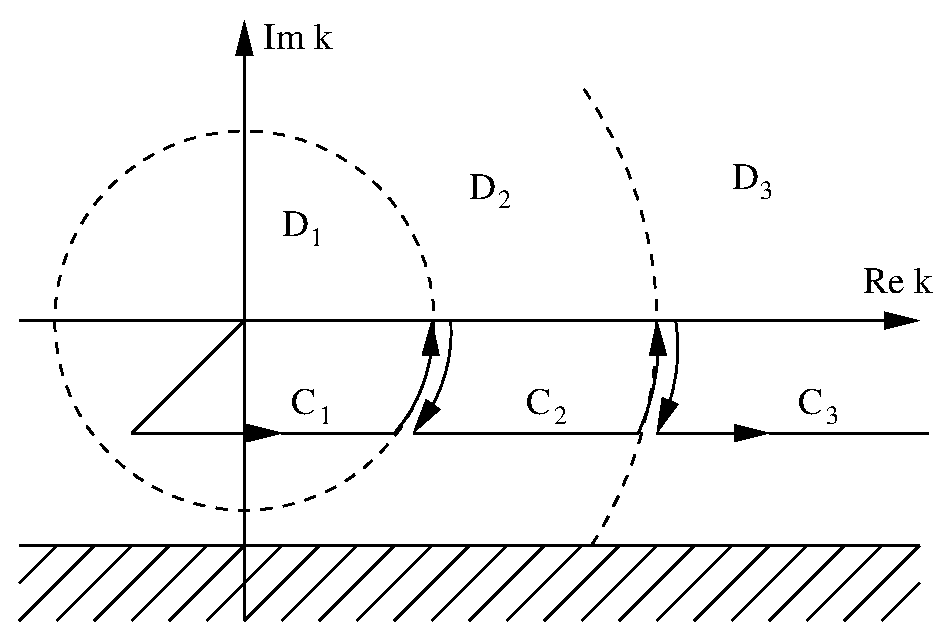
\epsfig{file=figures/medium1.eps}}
\end{center}
\caption{ $D_{1}$, $D_{2}$ and $ D_{3} $ demarcated by dotted circles 
define the regions in the complex    $ k$ -plane 
where the Pauli operator is analytic. The shaded area represents a region in the�
complex $k$-plane where singularities in the potential appear. The optimal  
deformed contour choice for equation~(\ref{eq:eigenvalue3}) is given by $  C = C_{1} + C_{2} + C_{3} $.}
\label{fig:medium1}
\end{figure}
The transformed equation~(\ref{eq:eigenvalue3}) will on the distorted contour $C$ take the form
\begin{equation}
\label{eq:transformed} 
\bar{H}_{0}(k,K) \psi_{nl}^{\alpha} (k,K ) + \bar{Q}(k,K;k_{f})\int_{C} 
dk' {k'}^{2}V_{l}(k,k')\psi_{nl}^{\alpha}(k',K) = E_{nl}^{\alpha}\psi_{nl}^{\alpha}(k,K)
\end{equation}
here $k$ and $k'$ are both defined on the contour $C$, giving a closed integral equation. 
The fermi momentum, $k_{f}$, and the center
of momentum, $K$, is kept real, since equation~(\ref{eq:transformed}) is an integral equation in the relative
momentum $k$ only. 
The normalization of the 2p2h states follow the generalized $c$-product as described for 
the free scattering case. 

\subsection{Pairing instabilities and resonance-like phenomena for the CD-Bonn interaction.}
Here we give a numerical calculation of 2p2h pair states in symmetric nuclear matter
using the realistic CD-Bonn \cite{machleidt} nucleon-nucleon interaction.
We use a free single particle spectrum with no gap in the calculations.
The 2p2h complex pole trajectories of the virtual states in the 
${}^1S_0$ channels are considered with increasing fermi momentum ($k_f$) and center
of momentum ($K$).
The 2p2h eigenvalue 
problem is solved on the contour $C$ consisting of a rotated and a translated part as 
shown in figure~\ref{fig:medium1}.
The singularity structure of the interaction is the same as for free scattering, 
the only modification is the angle averaged Pauli operartor entering the integral equation
\footnote{See Paper I for a discussion of the singularity structure of the CD-Bonn potential}.   
Figure~\ref{fig:1s0pole} gives the $^1S_0$ 2p and 2h complex pair states for $K = 0$ MeV and increasing
fermi momentum. Observe that the 2p2h pair states approaches the $^1S_0$ virtual states 
as $k_f \rightarrow 0 $. For $K = 0$ MeV the 2p2h pair states are located in the upper half 
complex $k$-plane. In this case integration along the real $k$-axis will give the 
complete energy spectrum, see figure~\ref{fig:1s0pole}. 
It is worth noting that the imaginary part of the 2p2h complex energy fits remarkably well 
with the pairing gap obtained from the BCS gap equation using a free single particle spectrum, 
see e.g. Ref.~\cite{morten2}.
This serves to illustrates that the BCS gap equation is an approximate solution of the 
2p2h eigenvalue problem as pointed out in Ref.~\cite{dick1,dick2,dick3} 
\begin{figure}[hbtp]
\begin{center}
\resizebox{9cm}{7cm}{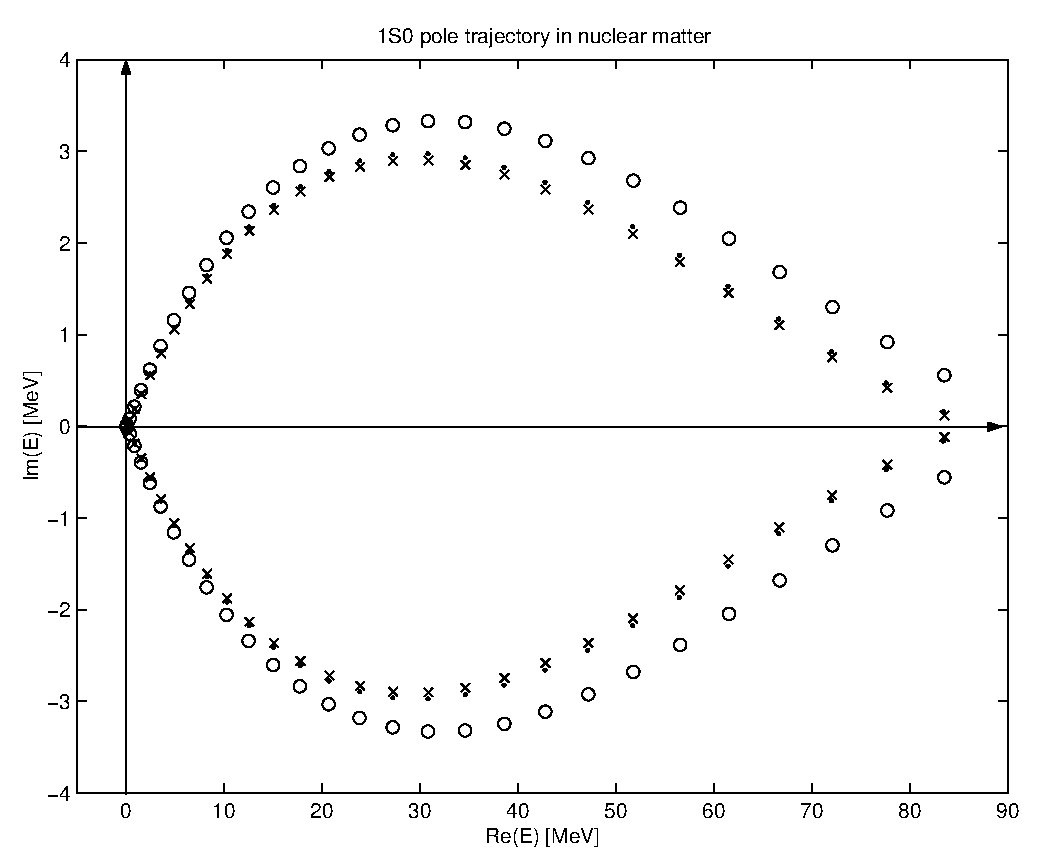
\epsfig{file=figures/1s0pole.eps}}
\end{center}
\caption{$^1S_0$ 2p2h pole trajectory in nuclear matter for $K_{CM}= 0$. 
Crosses:  $t_z = -1 $ -channel, dots: $t_z= 1$ , 
circles:  $t_z = 0$. $k_f \in [0, 280] $ MeV, $ \Delta k_f = 10$ MeV.}
\label{fig:1s0pole}
\end{figure}
Pairing correlations may also appear for $K > 0$.
Figure~\ref{fig:1s0virtual}�gives the $^1S_0$ 2p complex pole trajectory for increasing 
center of momentum and fixed fermi momentum. The complex pole move towards the real energy 
axis and eventually through the branch cut and 
onto the non-physical energy sheet with increasing center of momentum.
Translated to the momentum plane, this implies that  
the complex pole will move from the upper half $k$-plane and onto the lower half complex $k$-plane 
for a given center of momentum $K_{min}$. In the case $K > K_{min}$ the complete 2p2h 
energy spectrum is no longer obtainable by integrating along the real $k$-axis. 
By a suitable choice of contour CDM provides a method for obtaining the 
complete 2p2h energy spectrum for any $K > K_{min}�$.  
\begin{figure}[hbtp]
\begin{center}
\resizebox{9cm}{7cm}{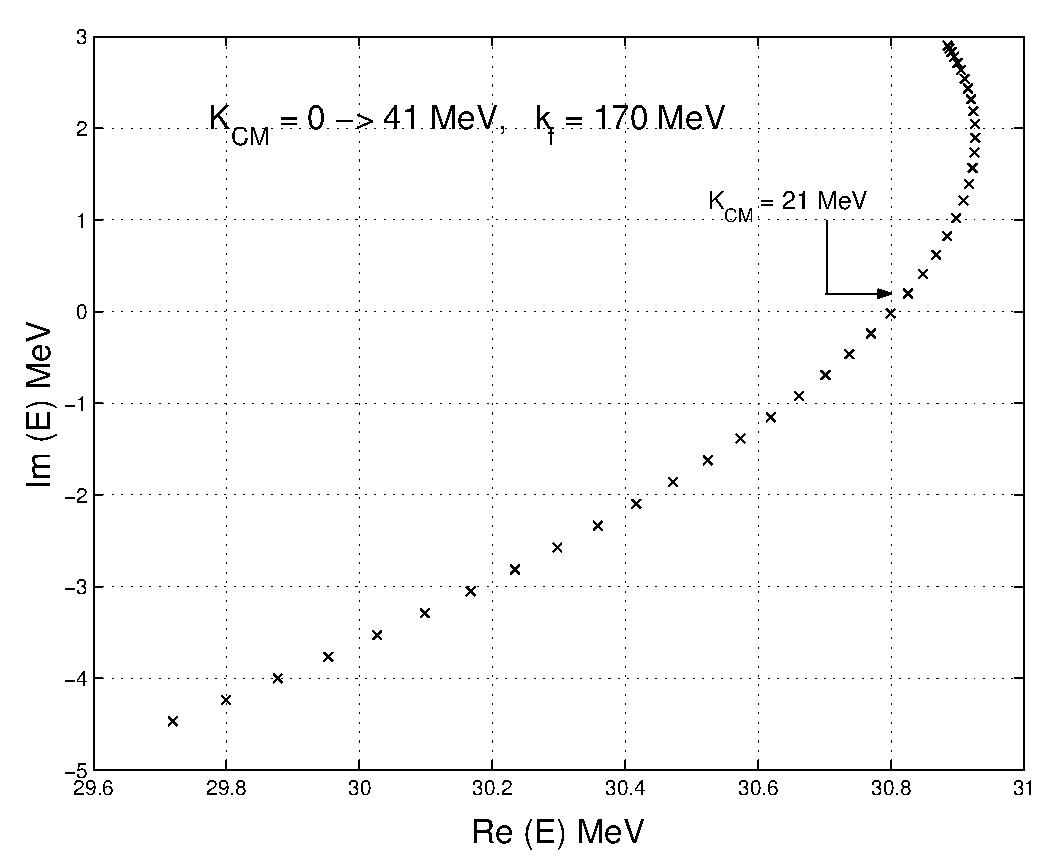
\epsfig{file=figures/1S0virtual.eps}}
\end{center}
\caption{Calculated 2p pole trajectory for maximum pairing instability $k_{f} = 170$ MeV in 
the $^1S_0 $ neutron - neutron isospin channel as function of $K_{CM}$. A rotated + translated contour 
was used in order to obtain energy spectrum. }
\label{fig:1s0virtual}
\end{figure}
Figure~\ref{fig:poles1} gives a scetch of the $^1S_0$ 2p2h pole trajectories in nuclear matter. 
First the center of momentum is held fixed and equal $K = 0$ and the fermi momentum is varied. 
The 2p and 2h poles will move symmetrically to the imaginary axis in the upper half complex
$k$-plane. Thereafter the fermi momentum is held fixed and the center of momentum is varied $K > 0$.
In this case the 2p and 2h poles will move towards the real $k$-axis and for a given $K$ into the
lower half complex $k$-plane.   
\begin{figure}[hbtp]
\begin{center}
\resizebox{9cm}{7cm}{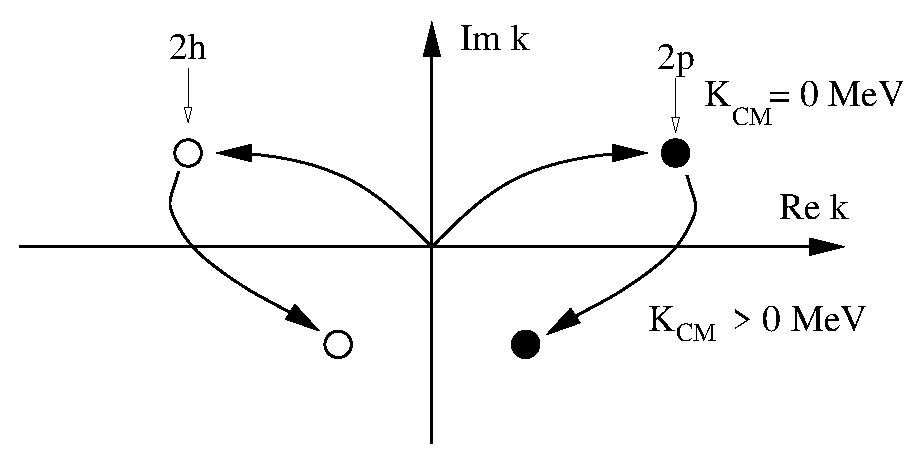
\epsfig{file=figures/poles1.eps}}
\end{center}  
\caption{Trajectory of 2p2h complex poles (pair instabilities) in 
nuclear matter for increasing fermi momentum, $k_{k}�$, and $K_{CM}�= 0$ MeV. 
The figure also give the trajectory for increasing center of momentum $K_{CM}$, and
$k_f$ is held fixed.}
\label{fig:poles1}
\end{figure}


\subsection{Calculation of $\Gamma $ by CDM for the CD-Bonn nucleon-nucleon interaction.}
In this section we will discuss a method for solving the full off-shell
vertex function (effective interaction), $\Gamma$, in a nuclear medium.
This method is based on analytic continuation of the integral equations and
expansion of the Green`s function on a complete set of Berggren states. This is
known as the Lehmann representation of the effective interaction $\Gamma $.
 
For two nucleons in free space the vertex function reduces to 
the  $t$-matrix, and hence the free full two-body scattering problem. 
In free space the $t$-matrix can be interpreted as an effective interaction
between two nucleons. In a scattering process the $t$-matrix
includes repeated two body interactions to infinite order, i.e. a summation of
all ladder diagrams to infinite order. In analouge to the free scattering case, 
we will consider only repeated interactions between either hole or particle states in 
the medium, giving the 2p2h ladder summed vertex function, $\Gamma $. 

The integral equation (\ref{eq:effective1}) for the effective interaction may be
written in relative and center of momentum coordinates by
\begin{equation}
\label{eq:gamma_mat1}
\Gamma_l(k,k'; \omega) = V_l(k,k') + \int_{0}^{\infty}dq q^2 V_l(k,q)
g_{II}^{FG(0)}(q,\omega)\Gamma_l(q,k'; \omega)  
\end{equation}
where we introduce the shorthand notation $\Gamma_l(k,k'; \omega) = \Gamma_l(k,k',K,k_f; \omega) $. 
The non-interacting 2p2h propagator is given, 
\begin{equation}
  g_{II}^{FG(0)}(k,\omega) = {\bar{Q}(k,K;k_f)\over \omega - H_0(k,K) }
\end{equation}
In the case of free scattering $Q=1$, and equation~(\ref{eq:gamma_mat1}) reduces
to the Lippmann-Schwinger equation for the $t$-matrix given in equation~(\ref{eq:tmat3}). 
The spectral representation of the effective interaction takes the following form
in RCM coordinates
\begin{equation}
  \label{eq:gamma_mat2}
  \Gamma_l(k,k'; \omega) = V_l(k,k') + \int_{0}^{\infty}dq q^2 
  \int_0^\infty dq' {q'}^2 V_l(k,q) g_{II}^{FG}(q,q';\omega) V_{l}(q',k')
\end{equation}
where the interacting 2p2h propagator is given by equation~(\ref{eq:int_prop}).
We will consider the solution of
Equation~(\ref{eq:gamma_mat2}) for the effective interaction by CDM. 
Using the completeness relation defined on a distorted contour $C$, shown in figure~\ref{fig:medium1}, 
gives the Berggren representation of the effective interaction in a nuclear medium, 
\begin{equation}
\Gamma_l(k,k'; \omega) = V_l(k,k') + \int_C dz z^2 
\int_C dz' {z'}^2 V_l(k,z) g_{II}^{FG}(z,z';\omega) V_{l}(z',k')
\end{equation}
here the interacting 2p2h propagator are represented in the 2p2h basis obtained by 
solving the eigenvalue problem in equation~(\ref{eq:transformed}).

By applying CDM and the spectral representation of the effective interaction,
we are able to single out the bound and resonant state contribution from the non-resonant 
2p2h continuum contribution  to the full effective interaction. 
The effective interaction may be written in the form,
\begin{displaymath}
\Gamma(\omega) = V + \Delta\Gamma(\omega) = V + \Delta\Gamma^R(\omega) + \Delta\Gamma^C(\omega), 
\end{displaymath}
here $R$ denotes the discrete bound and resonant states, $C$ denotes 
the non-resonant continuum contributions. 
In this way we may study the resonant, $\Delta\Gamma ^{R}$, and non-resonant 
contributions, $\Delta\Gamma ^{C}$, to the effective interaction separately. 
In figure~\ref{fig:eff} the effective interaction $\Gamma $ 
for the input energy $ \omega = ( k^2 + K^2 )/2m_{n} $, center of momentum 
$K=30$MeV and Fermi momentum $k_f=170$MeV 
is given for   $^1S_0$ neutron-neutron channel in the CD-Bonn interaction. 
A sharp peak is observed around the Fermi surface, indicating the existence of 
bound pair states. In figure~\ref{fig:eff5} the non-resonant continuum contribution 
to the effective interaction is plotted, and it is seen that the peak 
around the Fermi surface has disappeared. The Discontinuties in the non-resonant
contribution is due to the analytic structure of the angle averaged Pauli operator given 
in equations.~(\ref{eq:pauli1},\ref{eq:pauli2}, \ref{eq:pauli3}). In figure~\ref{fig:eff6}
the resonant contribution to the effective interaction is given.
The resonant contribution displays a sharp peak around the Fermi surface, 
while the resonant contributions are neglible moving away from the Fermi surface.
 
In conclusion, CDM will enable us to 
obtain $\Gamma_{l}(k,k',K;\omega) $ for both real and complex input energies $\omega�$. 
The integral becomes non-singular on the deformed contour for real 
input energies $\omega $, resulting in numerically stable solutions for
two-body scattering in both free space and in a uniform medium.   
In this perspective, CDM offers an alternative approach to the standard
PV prescription in solving for the effective interaction, and
offers a valuable tool in descrbing different contributions to the
effective interaction.
\begin{figure}[hbtp]
\begin{center}
\resizebox{9cm}{7cm}{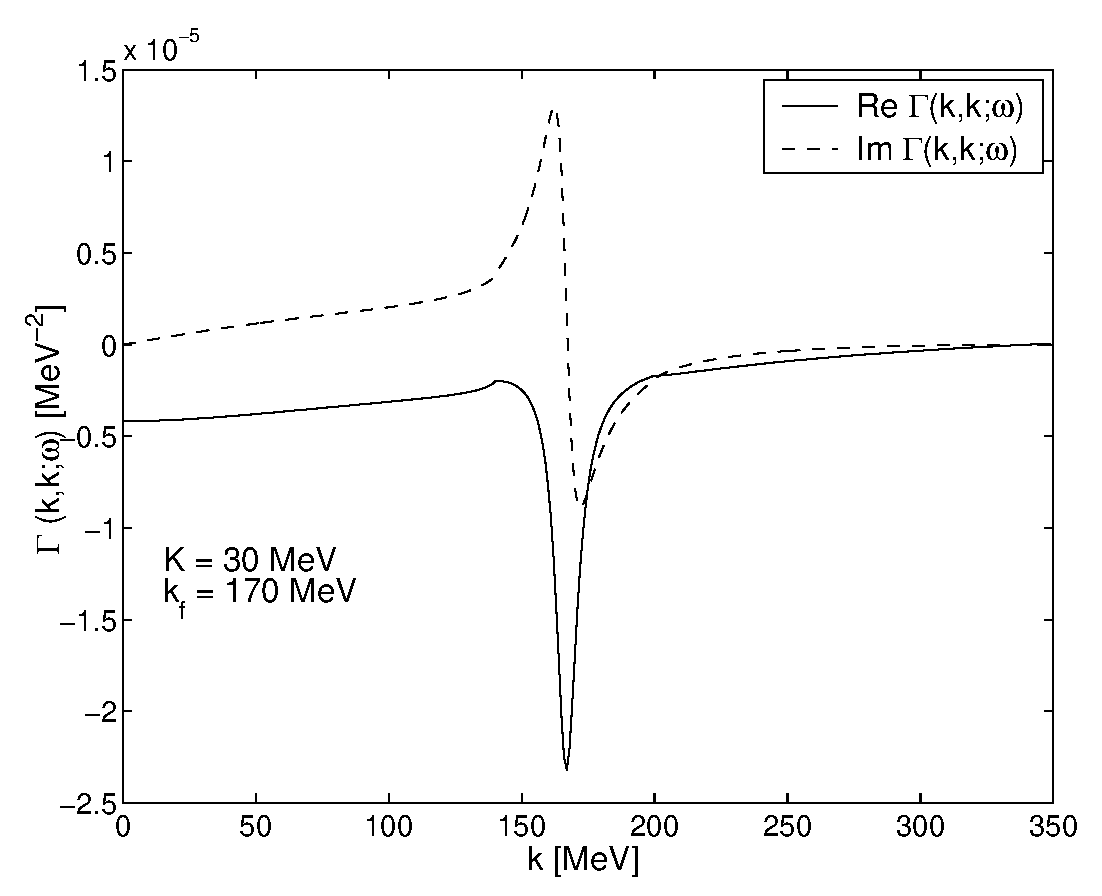
\epsfig{file=figures/eff.eps}}
\end{center}  
\caption{Effective interaction $\Gamma(k,k; \omega = ( k^2 + K^2 )/2m_{n} )  $ for $K = 30$ MeV and 
$k_f = 170$ MeV for $^1S_0$ neutron-neutron channel in the CD-Bonn interaction. The peak around 
the fermi surface $k \approx 170 $MeV indicates the formation of a pairing instability. }
\label{fig:eff}
\end{figure}

      
\begin{figure}[hbtp]
\begin{center}
\resizebox{9cm}{7cm}{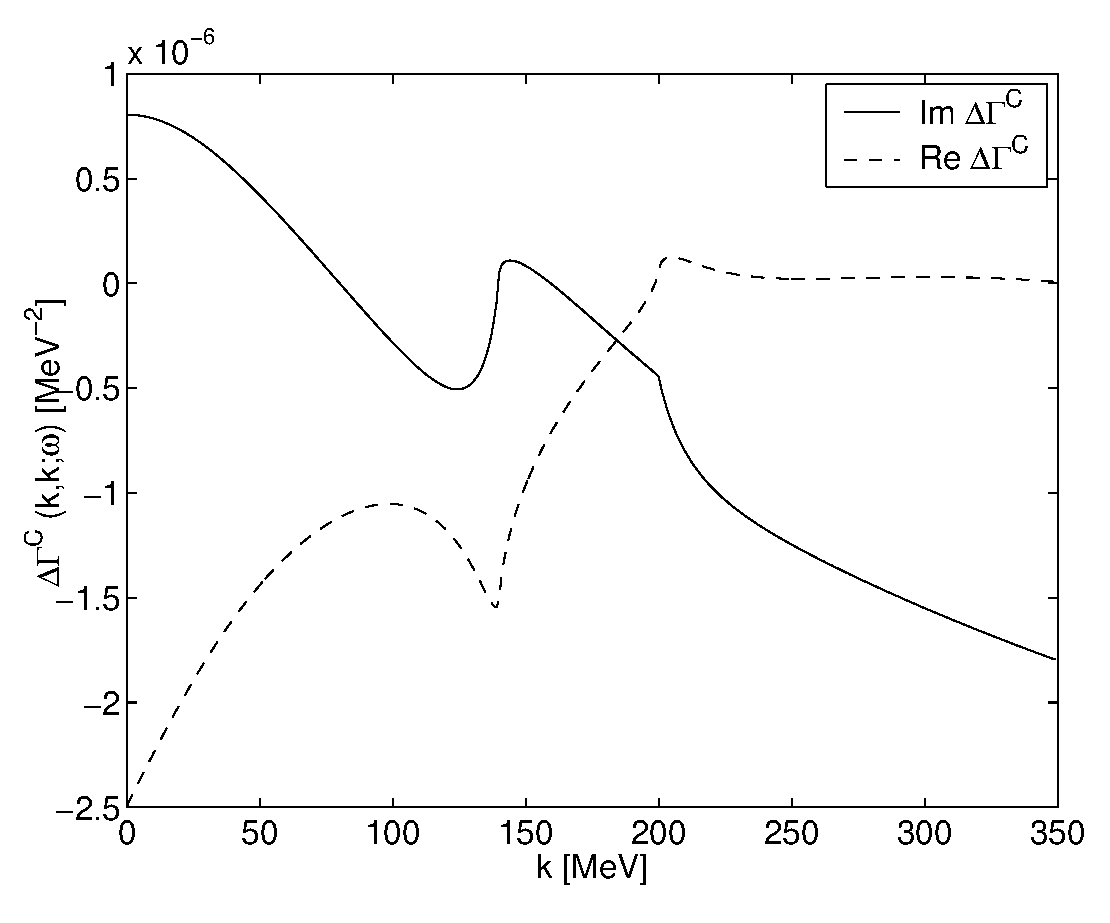
\epsfig{file=figures/eff5.eps}}
\end{center}  
\caption{Continuum part of effective interaction $\Delta\Gamma(k,k; \omega = ( k^2 + K^2 )/2m_{n} )  $ 
for $K = 30$ MeV and 
$k_f = 170$ MeV for $^1S_0$ neutron-neutron channel in the CD-Bonn interaction. The peak around 
$k \approx 170 $MeV has been washed out. }
\label{fig:eff5}
\end{figure}


\begin{figure}[hbtp]
\begin{center}
\resizebox{9cm}{7cm}{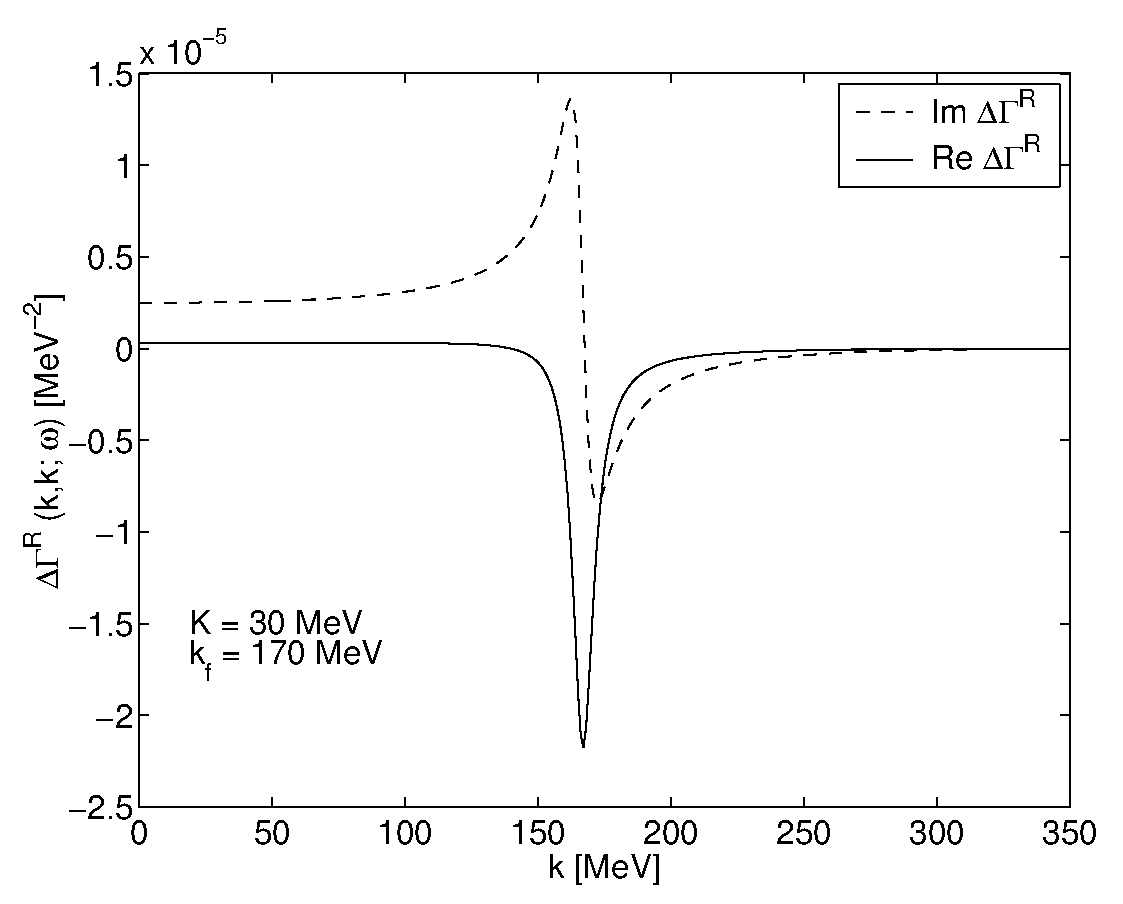
\epsfig{file=figures/eff6.eps}}
\end{center}  
\caption{Resonant part of effective interaction $\Delta\Gamma(k,k; \omega = ( k^2 + K^2 )/2m_{n} )  $ 
for $K = 30$ MeV and 
$k_f = 170$ MeV for $^1S_0$ neutron-neutron channel in the CD-Bonn interaction. The resonant part of $\Gamma $
has is clearly non-neglible around the fermi surface $k \approx 170 $MeV. }
\label{fig:eff6}
\end{figure}


 
\chapter{Effective interactions and many-body theory for unstable nuclei}

% new section
\section{The Gamow shell model}
\label{sec:gamow_shell_model}
The standard nuclear shell model often starts with a harmonic oscillator
representation for the single particle states. 
Since the harmonic oscillator potential 
is an infinite potential, the tail in single particle wave function 
falls off to rapidly in order to describe realistically 
single particle motion near the scattering continuum. The harmonic
oscillator may therefore be said to work only for deeply bound nucleons. 
In order for the nuclear shell model to be applicable to nuclei 
far from the valley of stability, the harmonic oscillator picture 
of single particle motion has to be abdoned. The proximity of the
scattering continuum in  loosely bound and unbound nuclei, necessitates
a modification and reformulation of the standard nuclear shell model.

From the previous sections, it was shown how a single particle
basis consisting of bound, anti-bound and resonant states may be
constructed using the Contour Deformation Method in momentum space. 
Solving the momentum space integral equation on a discretized
contour in the complex $k$-plane a complex symmetric eigenvalue
problem for the single particle states 
where obtained, and from which a complete set of
\emph{bi-orthogonal} states follows. Since the basis 
is discretized on a deformed contour it is possible
to assign a unique quantum number to each single particle state.
In the case of harmonic oscillator 
states we have the usual notation for the quantum numbers
$(n,l,j) $ where $n$ is nodal number and $(lj)$ the orbital- 
and total angular momentum of the single particle state.
In the general case where bound, anti-bound, resonances and
non-resonant continuum states are treated on equal footing, 
the meaning of the quantum number $n$ has to be redefined and 
clarified. Since all single particle states have a discrete energy 
associated with them, it is natural to let $n$ refer to
the $n$'th discrete energy $E_n$. Defining $n$ is manner, all 
single particle states have a unique set of quantum number $n,l,j$.
figure~\ref{fig:sp_orb}�illustrates how $N$ single particle Berggren orbitals for 
a given $(lj)$ partial wave,
obtained by solving the momentum space Schr\"odinger equation on a $N$-point 
discretized contour in the complex $k$-plane, 
may be organized in an ordered way. The non-resonant continuum orbitals are
distinguished from the discrete bound- and resonant orbitals. 
\begin{figure}[hbtp]
\begin{center}
\resizebox{11cm}{6cm}{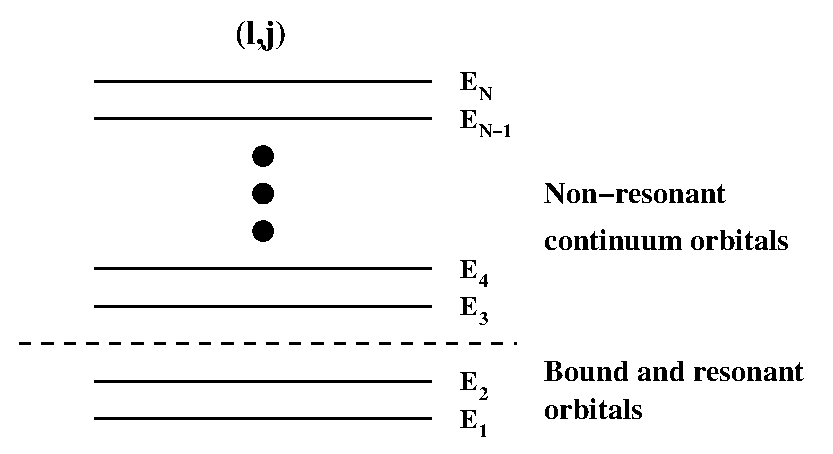
\epsfig{file=figures/sp_orbitals.eps}}
\end{center}
\caption{Illustration of how the bound, resonant and non-resonant continuum 
orbitals for a given $(lj)$ single particle configuration may be organized in 
an ordered way.} 
\label{fig:sp_orb}
\end{figure} 
Having constructed a single-particle Berggren basis, a many-body Berggren basis
may be constructed in a completely analogous way as when 
harmonic oscillator states are used. We construct a complete anti-symmetric 
$N$-body basis from the Slater determinants consisting of the 
Berggren orbitals $\varphi_{nljm}�$ 
i.e. 
\begin{equation}
  \Phi_{\alpha_1,...,\alpha_n}(1,...,n) = {1\over \sqrt{n !}}
  \left| \begin{array}{ccc} 
    \varphi_{\alpha_1}(1) & \ldots &  \varphi_{\alpha_1}(n) \\
    \vdots &  & \vdots \\
    \varphi_{\alpha_n}(1) & \ldots &  \varphi_{\alpha_N}(n) 
    \end{array}\right|,
\end{equation} 
where $\alpha_i$ labels the single particle quantum numbers $(n_il_ij_im_i)$. 
The Slater determinant have eigenvalues 
$E_{i}�= \varepsilon_{\alpha_1} + ... + \varepsilon_{\alpha_N}$, which is just the sum 
of all single particle energies. Here�the label $i$ subsumes all the 
different single particle quantum numbers 
$ \varepsilon_{\alpha_1} + ... + \varepsilon_{\alpha_N}$.
We then have at hand a complete set of $N$ many-body Slater determinants, i.e.
\begin{equation}
  1 = \sum_i^N \vert \Phi_i \rangle \langle \Phi_i^*\vert,
\end{equation}
which the exact many-body wave function may be expanded in. 
The shell model problem then
requires the solution of a complex symmetric $N\times N$
matrix eigenvalue equation,  
\begin{equation}
  H \vert \Psi_i \rangle = E_i \vert \Psi_i \rangle, 
\end{equation}
with $i = 1,...,N$. Representing the shell model states in a complete set of 
Slater determinants, built from 
the single particle orbitals with quantum numbers $(nljm)$, 
is commonly known as the $m$-scheme representation.  The Slater 
determinants are antisymmetric and have definite values of the total 
spin projection $M_J = m_1+m_2+...+m_n $ and total isospin projection  
$M_T = \tau_1 + \tau_2 +...+\tau_n$, but they are not states with 
good quantum number of total spin $J$ and isospin $T$. In 
standard large-scale shell model calculations, using the the $m$-scheme representation, 
one is typically interested
in the the first few low lying energy states. The Lanczos algorithm \cite{lanczo}   
is an iterative method which has proven to be efficient in solving for a limited set 
of eigenvalues of large real symmetric matrices. 

In the Gamow Shell Model case, the $m$-scheme and the standard Lanczos iterartion
technique for solving large eigenvalue problem for real symmetric matrices are not 
optimal approaches. Firstly, the $m$-scheme representation 
of the shell model equations does not automatically split the 
full shell model matrix into 
smaller sub-martices for different values of the total spin $J$ 
and isospin $T$. In standard shell model calculations only bound states appear, 
but in Gamow Shell Model, not only bound states but a rather large set 
of continuum states are included for each $lj$ configuration. 
In a $m$-scheme represenation, the dimension of the matrix will, 
in the Gamow Shell Model case, in most cases be too large 
to handle numerically. 
On the other hand, one may construct a  
many-body basis coupled to definite total spin $J$ and $T$, either by
the $j-j$ or the $L-S$ coupling scheme. Thereafter the shell model 
equations for a given value of spin and isospin may be
diagonalized separately.  The dimension of each $J,T$ 
matrix will then be considerably smaller than the full 
matrix represented in the $m$-scheme.  For Gamow Shell Model
calculations the $j-j$ or the $L-S$ coupling scheme seems to be the 
most suitable representations.
Secondly, the Lanczos iteration method has usually been used for 
calculation of a set of eigenvalues lowest in real energy. 
In Gamow Shell Model calculations there may be  a large 
number of complex continuum states
lying below the physical resonances in real energy.
In addition it is difficult to
predict where the multi-particle resonances will appear after diagonalization. 
Direct diganalization procedures has to be abdoned, since
the matrices with increasing number of valence particles soon become 
too large to store and handle on most modern computers. 
However, as will be shown in the next section, the Lanczos iteration technique
may be generalized to complex symmetric matrices. Choosing 
a reasonable initial Lanczos vector for the multi-particle resonance, 
it will be shown that the Lanczos iteration procedure gives accurate
and converged results for the multi-particle resonance 
with a fairly small number of iterations. 

Choosing to work Slater determinants coupled to definite spin, 
the $N-$body anti-symmetric wave function can be constructed viz., 
\begin{equation}
  \Psi_\alpha^{JM} (1,...,N) = \sum_{i} C_{i}^{JM} {\Phi}_{i}^{JM}(1,...,N), 
  \label{eq:twobody_antisym}
\end{equation}
where the indice $i$ represent the various single-particle orbits.
Here ${\Phi}_{i}^J(1,...,N) $ is a normalized $N-$body anti-symmetric 
wave function.  The shell model equations we have to solve is then given 
by 
\begin{equation}
  H \vert \Psi_i^J \rangle = E_i^J \vert \Psi_i^J \rangle, 
\end{equation}
In our Gamow Shell Model studies of $^{6-7}$He 
in Paper II, we worked within the $j-j$ coupling scheme. See 
Appendix~\ref{sec:3matel} for the derivation of 
three-body matrix elements in $j-j$ coupling.
Table~\ref{tab:dimension} gives the various dimension for the 
shell model matrices with definite spin and parity $J^\pi$ for
the different $^{5-7}$He isotopes considered in Paper II. 
It is seen that with a valence space of 24 $p_{1/2}$ and 24 $p_{3/2}$ 
single particle orbitals, the dimension grows extremely fast with 
increasing number of valence particles. Even in the case of three valence
particles the dimension is too large for direct diagonalization procedures. 
This problem of the dimensionality of the Gamow Shell Model equations
is what we call the \emph{dimensionality problem}. 
\begin{table}[htbp]
  \begin{center}
  \begin{tabular}{cccccc}
    \hline
    \multicolumn{2}{c}{$^5$He} & \multicolumn{2}{c}{$^6$He} 
    & \multicolumn{2}{c}{$^7$He} \\
    \hline
    \multicolumn{1}{c}{$J^\pi$} &  \multicolumn{1}{c}{$N$}& 
    \multicolumn{1}{c}{$J^\pi$} &
    \multicolumn{1}{c}{$N$} & \multicolumn{1}{c}{$J^\pi$ } &
    \multicolumn{1}{c}{$N$} \\
    \hline
    ${1/2}^-$ & 24 & $0^+$ & 600  & ${1/2}^- $ & 29648 \\
    ${3/2}^-$ & 24 & $1^+$ & 1128 & ${3/2}^- $�& 38896 \\
       {}     & {} & $2^+$�& 876  & ${5/2}^- $ & 27072 \\
    \hline
  \end{tabular}
  \caption{Dimension of the shell model matrices with definite spin and parity $J^\pi $ 
    for the $^{5-7}$He isotopes.}
  \label{tab:dimension}
  \end{center}
\end{table}
In order to be able to solve for the eigenvalue 
spectrum of such large complex matrices, 
effective interaction techniques and matrix perturbation theory 
generalized for complex symmetric matrices have to be developed and studied. 
This is the topic of the next sections.


\section{Lanczos iteration process for many-body resonances.}
\label{sec:lanczo}
The Lanczos iteration technique for finding a limited 
set of eigenvalues and eigenvectors for large real matrices, 
has over the years been the dominating approach in solving large-scale
shell model equations. The 
method may easily be generalized to apply for complex matrices. This suggest that 
the method may be a suitable approach for dealing with 
large complex symmetric matrices which appear in Gamow Shell Model
studies. However, we need a reliable prescription for
identifying which state is to be associated with the physical
multi-particle resonance from the set of eigenvectors obtained
from diagonalizing the Lanczos matrix. Below we shall show 
how such a prescription may be defined. As a test case 
we consider the bound and resonant spectra of $^6$He, using 
a shell model picture with two valence neutrons moving in $p_{3/2}$ 
Berggren orbitals outside a  $^4$He core. We use 24 single discretization points 
for the contour in generating the $p_{3/2}$ single particle basis of $^5$He. 
See Paper II for further details on the contour, the $^4$He -$n$ 
interaction potential and
on the residual nucleon-nucleon interaction for the two valence nucleons. 

The many-body basis in which we expand the shell model wave function, 
is constructed from Slater determinants built from  the single 
particle Berggren orbitals in a given valence space, and coupled to total 
spin $J$�since we work in a $j-j$ coupling scheme.
corresponding Hamiltonian may be represented in this basis. 
For the Lanczos iteration scheme to converge rapidly, the
choice of a 0th order approximation to the multi-particle resonance should
resemble the exact multi-particle resonance as much as possible. Constructing
a reasonable starting vector for the Lanczos iteration procedure, is 
what we have to consider firstly. Having constructed a complete many-body 
basis from the single particle Berggren orbitals, the many-body space
may be partioned into a model space $P$ and an orthogonal complement space
$Q$ by some selection procedure. 
The shell model Hamiltonian may then
subsequently be partioned into two parts according to, 
\begin{equation} 
H =  \left( \begin{array}{cc}
    PHP & PHQ \\ 
    QHP & QHQ  
  \end{array} \right)  =  
  \left( \begin{array}{cc}
    H^{PP} & 0 \\ 
    0 & 0 
  \end{array} \right) 
  +
  \left( \begin{array}{cc}
    0 & H^{PQ} \\ 
    H^{QP} & H^{QQ}  
  \end{array} \right).
\end{equation}
The model space $P$ should be constructed in such a way that the most important 
many-body configurations of the many-body resonance wave function 
are included in this restricted space. Furthermore, the dimension $N_P$ of the model space
$P$ should be small enough so that a full diagonalization of $H^{PP} $ is possible.
The 0th order lanczos vector $\vert \mathrm{lanc}_0\rangle $, which is the 0th order 
approximation to the exact wave function,  is then obtained by diagonalizing 
the $N_P\times N_P$ model space matrix $H^{PP}$. In choosing the model space $P$ 
it is natural to assume that the most important configurations are those in which 
all or several particles are in single particle resonance orbitals. The $Q$-space 
consists then of the remaining configurations. In the $^6$He test case we
consider two different model spaces $P = P_1, \:P_2$. 
In the first case we let $P$ be given by a single Slater determinant, 
where both neutrons are in the $p_{3/2}$ single particle resonance orbital, 
i.e. $P_1 = \vert RR \rangle $. In this case the 
0th order lanczos vector is just the single Slater determninant,
\begin{equation}
  \vert \mathrm{lanc}_0 \rangle = \vert \Phi_i^J \rangle = \vert RR \rangle. 
  \label{eq:start1}
\end{equation}  
In the second choice we construct $P$ from all Slater determinants 
where at least one neutron is in the $p_{3/2}$ 
single particle resonance orbital, i.e.
\begin{equation}
  P_2 \equiv  \left\{ \vert RR \rangle, \vert RC\rangle \right\},
\end{equation}
and the corresponding model space dimension is $N_{P_2} = 24$. 
In this case the 0th order Lanczos vector is a linear combination of 
Slater determinants, 
\begin{equation}
  \vert \mathrm{lanc}_0\rangle = \sum_{i=1}^{N_{P_2}} C_{i,j}\vert \Phi_i^J \rangle.
  \label{eq:start2}
\end{equation}
Here $C$ is a $N_{P_2}\times N_{P_2}$   orthogonal matrix 
which diagonalizes $H^{PP}$. 
The orthogonal columns $j$ of $C$ have been 
normalized so that $\vert \mathrm{lanc}_0\rangle  $ is normalized.  
For each Slater determinant $\vert \Phi_i \rangle,\:\: i=1,...,N_{P_2}$  a corresponding 
amplitude $C_{i,j}$ is assigned. As the diagonalization of the model 
space matrix $H^{PP}$ 
gives $N_{P_2}$ possible choices for the 0th order 
Lanczos vector, we have to determine from this set 
which is the 0th order approximation 
to the exact two-particle resonance wave function. 
This may be done by considering each column $j$ of the matrix $C$, 
and determine which of these columns have the largest amplitude $C_{i,j}$ for
the Slater determinant where all particles are in single particle 
resonance orbitals.

The Lanczos iteration procedure may be summarized by the following steps,
\begin{enumerate}
\item Choose an initial Lanczos vector $\vert \mathrm{lanc}_0\rangle $ 
  ( a linear combination of Slater determinants ) as the 0th order approximation 
  to the exact multi-particle resonance wave function. See discussion above, on how 
  to choose this starting vector for Gamow Shell Model applications. 
\item The next step involves generating a new vector $ \vert \mathrm{new}_{p+1}\rangle $ 
  by letting 
  the full Hamiltonain $H$ act on the $p$'th Lanczos vector $\vert \mathrm{lanc}_p\rangle $, i.e. 
  $ \vert \mathrm{new}_{p+1}\rangle = H \mathrm{lanc}_p\rangle  $.
  Throughout this process we construct the energy matrix elements of $H$ 
  in this Lanczos basis. The diagonal matrix elements of $H$ are then 
  obtained by
  \begin{equation}
    \langle \mathrm{lanc}_p \vert H \vert \mathrm{lanc}_p \rangle = 
    \langle \mathrm{lanc}_p \vert \mathrm{new}_{p+1} \rangle.
  \end{equation}
\item The new vector $ \vert \mathrm{new}_{p+1} \rangle $ is 
  then orthogonalized to all previously calculated Lanczos vectors
  by the Gram-Schmidt procedure 
  \begin{equation}
    \vert \mathrm{new}_{p+1}' \rangle = 
    \vert \mathrm{new}_{p+1} \rangle - 
    \sum_{q=0}^p \vert \mathrm{lanc}_{q} \rangle 
    \langle \mathrm{lanc}_q \vert \mathrm{new}_{p+1}\rangle,
  \end{equation} 
  and normalized 
  \begin{equation}
    \vert \mathrm{lanc}_{p+1}\rangle = {1 \over 
      \sqrt{ \langle \mathrm{new}_{p+1}'\vert \mathrm{new}_{p+1}'\rangle }�}
    \vert \mathrm{new}_{p+1}'\rangle,
  \end{equation} 
  to give a new normalized Lanczos vector.
\item The off-diagonal matrix elements of $H$ is then obtained by
  \begin{equation}
    \langle \mathrm{lanc}_{p+1}\vert H \vert \mathrm{lanc}_{p}\rangle = 
    \langle \mathrm{lanc}_{p+1}\vert \mathrm{new}_{p+1}'\rangle,
  \end{equation}
  and all other matrix elements are zero. 
\item After $p$ iterations we have an energy matrix of 
  tridiagonal form 
  \begin{equation}
    \left[ \begin{array}{ccccc}
	H_{0,0} & H_{0,1} &   0     & \ldots & 0 \\
	H_{1,0} & H_{1,1} & H_{1,2} & \ldots & 0 \\
	0       & H_{2,1} & H_{2,2} & \ldots & 0 \\
	\vdots  & \vdots  & \vdots  & \vdots & H_{p-1,p} \\
	0       &   0     &   0     & H_{p,p-1} & H_{p,p} 
      \end{array} \right]
  \end{equation}
  as the $p$'th approximation to the full eigenvalue problem. 
  The number $p$ is a reasonably small number so the matrix
  can be diagonalized by standard diagonalization routines
  for sparse matrices of tridiagonal form, to obtain eigenvalues and 
  eigenvectors which are linear combinations of the Lanczos vectors. 
\item This process is repeated until a suitable convergence criterion has been
  reached.
\end{enumerate}
Having determined a converged Lanczos energy matrix, 
the remaining problem is how to determine which of the states
$\vert \Psi_i(p) \rangle, \:\: i = 1,...,p$ gives the 
$p$'th approximation to the exact multi-particle resonance.  
This identification may be done unambigously by determining 
which state $\vert \Psi_i(p) \rangle, \:\: i = 1,...,p$
has the largest overlap with the initial Lanczos vector $\vert \mathrm{lanc}_0\rangle $, 
which is the
0th order approximation to the exact multi-particle resonance.
\begin{figure}[hbtp]
\begin{center}
\resizebox{11cm}{9cm}{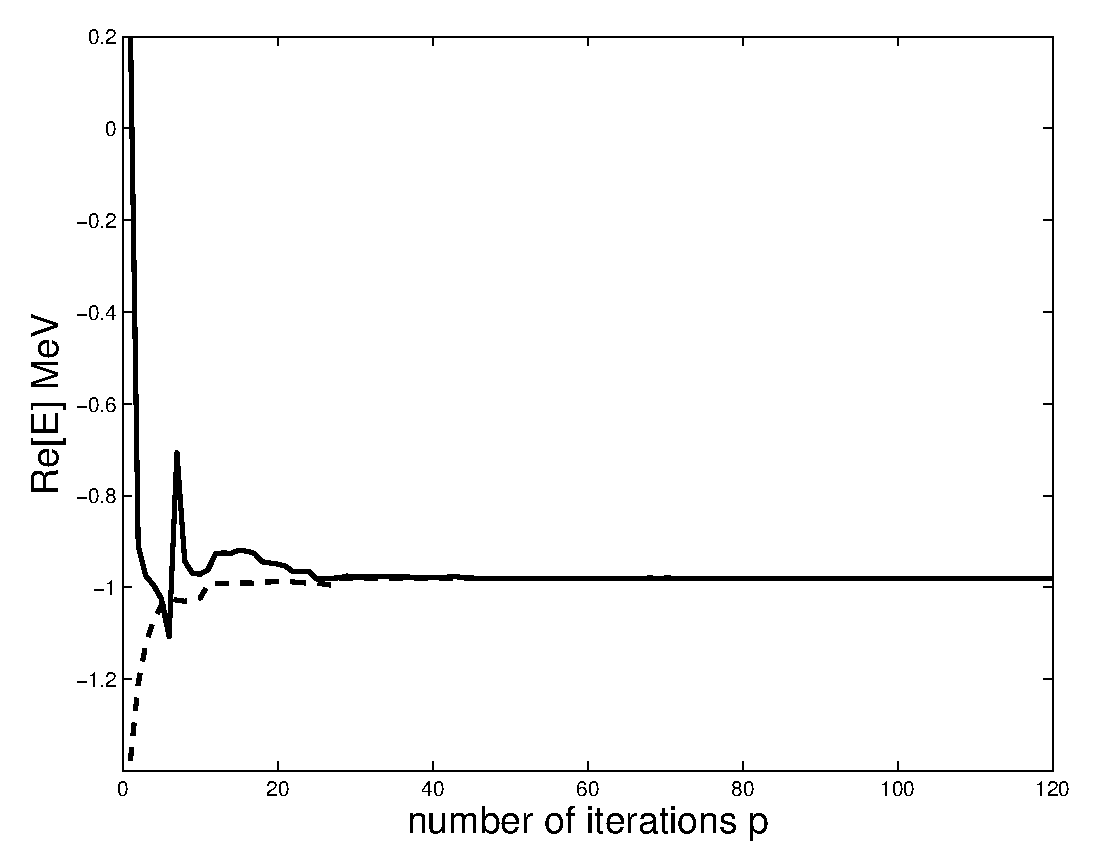
\epsfig{file=figures/lanczo1_re0plus.eps}}
\end{center}
\caption{Convergence of the real part of the $0^+$ ground state energy of $^6$He.} 
\label{fig:lanczo1}
\end{figure} 

\begin{figure}[hbtp]
\begin{center}
\resizebox{11cm}{9cm}{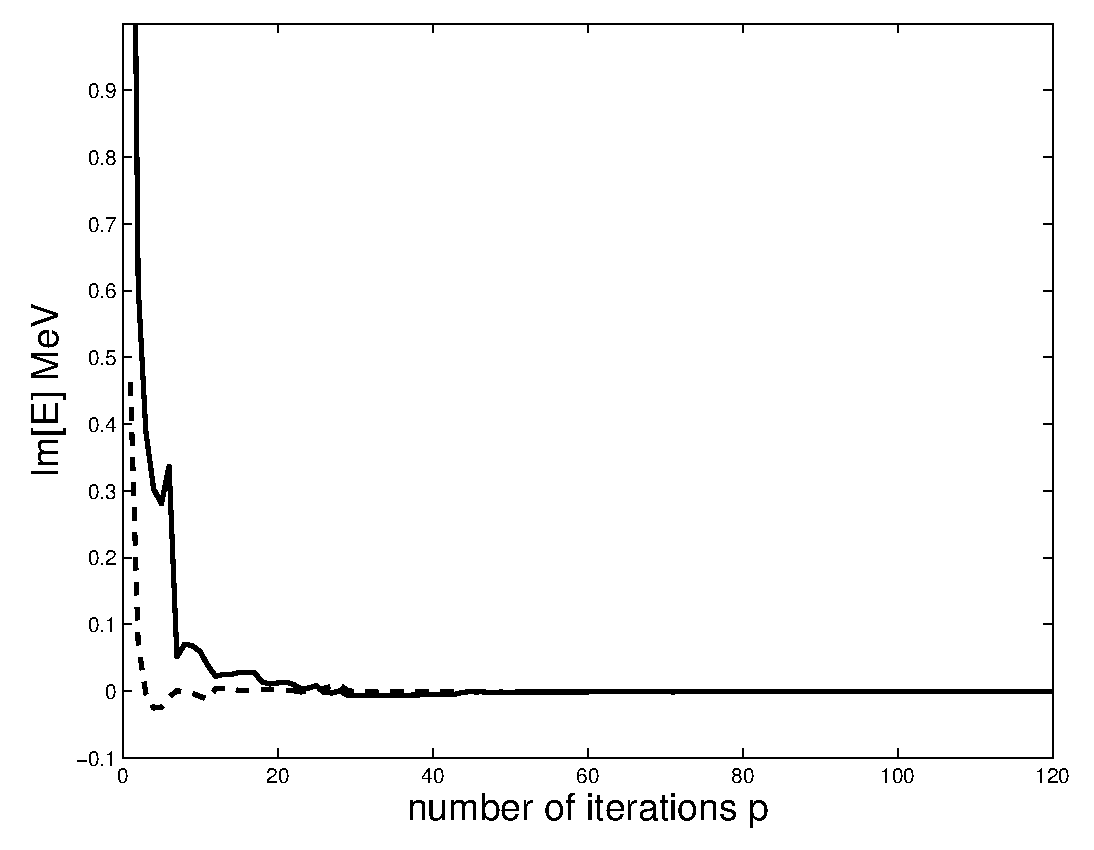
\epsfig{file=figures/lanczo1_im0plus.eps}}
\end{center}
\caption{Convergence of the imaginary part of the $0^+$ ground state energy of $^6$He.} 
\label{fig:lanczo2}
\end{figure} 

\begin{figure}[hbtp]
\begin{center}
\resizebox{11cm}{9cm}{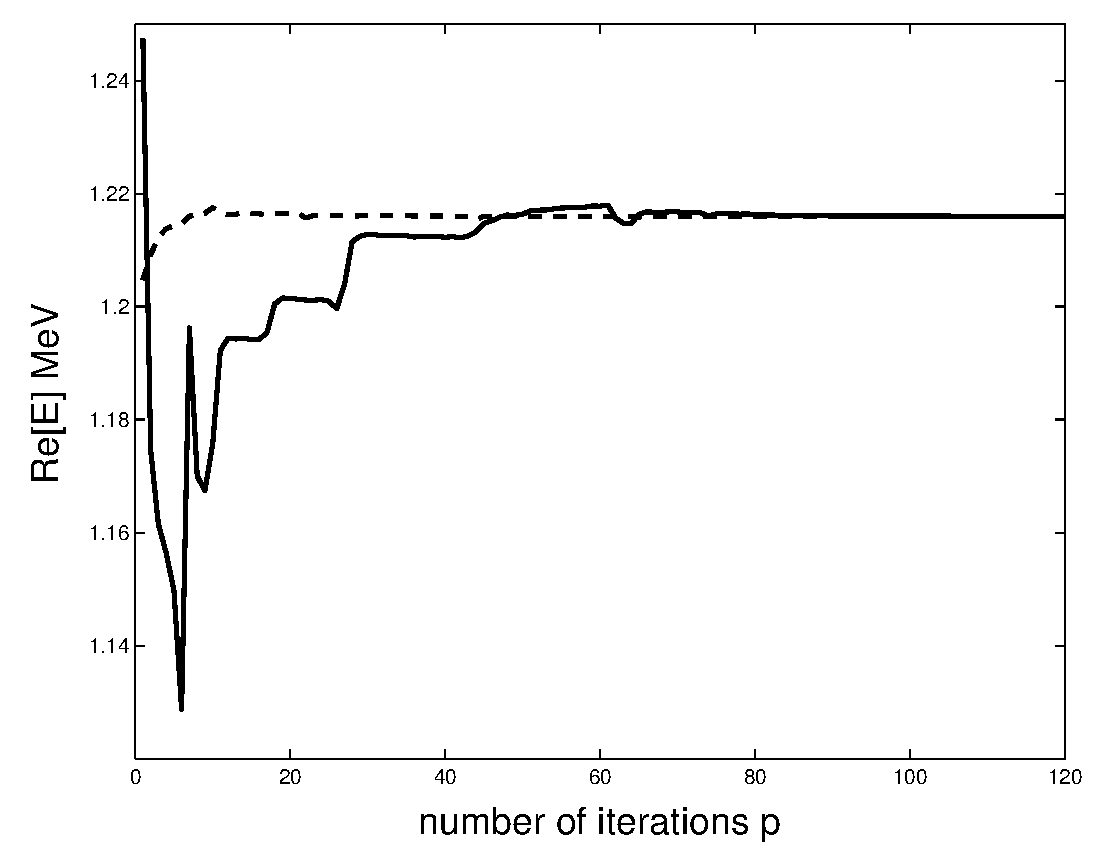
\epsfig{file=figures/lanczo1_re2plus.eps}}
\end{center}
\caption{Convergence of the real part of the $2^+$ resonance energy of $^6$He.} 
\label{fig:lanczo3}
\end{figure} 

\begin{figure}[hbtp]
\begin{center}
\resizebox{11cm}{9cm}{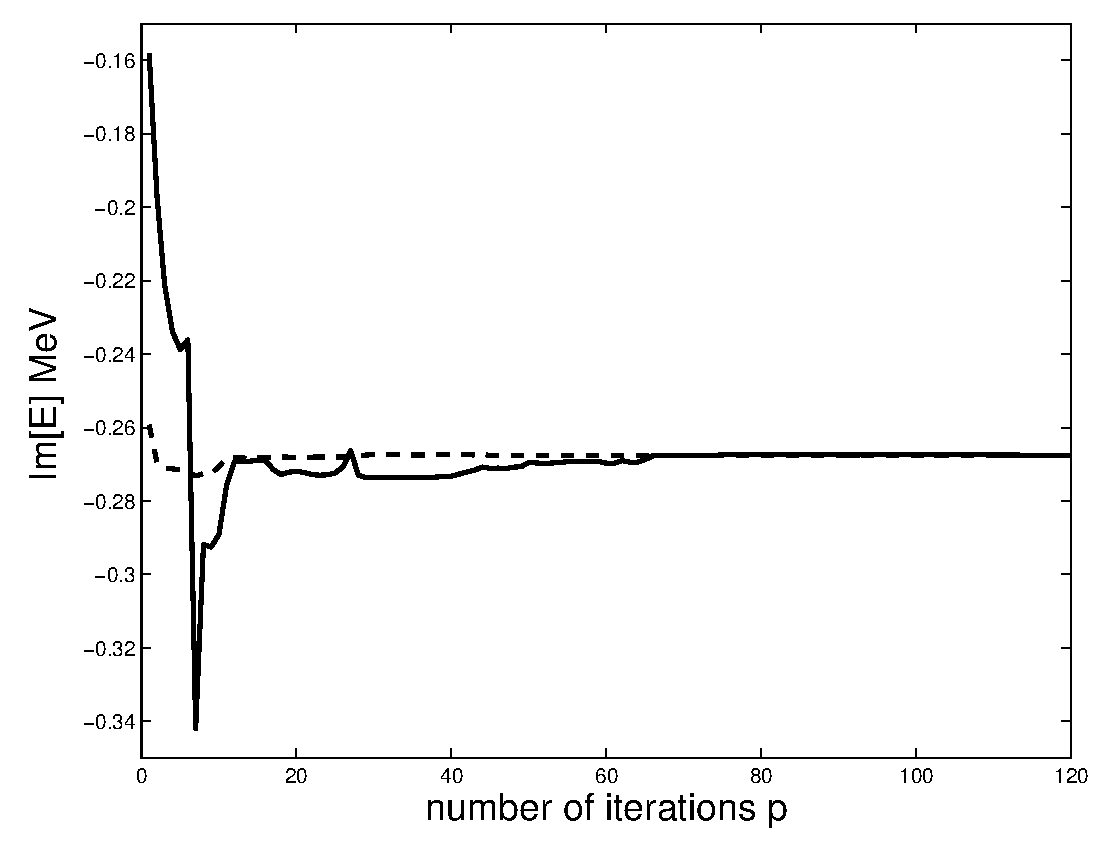
\epsfig{file=figures/lanczo1_im2plus.eps}}
\end{center}
\caption{Convergence of the imaginary part of the $2^+$ resonance energy of $^6$He.} 
\label{fig:lanczo4}
\end{figure} 

Figures~\ref{fig:lanczo1} and \ref{fig:lanczo2} 
gives the approximate real and imaginary parts of the
$0^+$ ground state of $^6$He obtained after $p$ iterations, 
using
the starting vector given in equation~(\ref{eq:start1}) (solid line) 
and the starting vector given in equation~(\ref{eq:start2}) (dashed line).
It is seen 
that both for the real and imaginary parts of the energy, 
the convergence is  faster for
the initial Lanczos vector given in equation~(\ref{eq:start2})
than compared with the convergence using the initial 
vector in equation~(\ref{eq:start1}). However, it is interesting to see that
both choices 
converges to the exact ground state energy $E(0^+) = -0.98 +0.00i $MeV 
within the number of iterations $p$ considered. 
Figures~\ref{fig:lanczo3} and \ref{fig:lanczo4} 
gives the approximate real and imaginary parts of the
$2^+$ resonant state of $^6$He obtained after $p$ iterations, using
the starting vector given in equation~(\ref{eq:start1}) (solid line) 
and the starting vector given in equation~(\ref{eq:start2}) (dashed line).
Also in this case convergence is faster using equation~(\ref{eq:start2}) 
for an initial Lanczos vector. Both choices converges to the 
exact two-particle resonance energy $E(2^+) = 1.216 - 0.268i$MeV for a reasonable
small number of iterations $p$.
This test study of  the Lanczos iteration procedure
applied to Gamow Shell Model studies, is very promising. 
Both resonances and bound states are reproduced with a 
small number of iterations, given a reasonable choice for
a 0th order approximation to the two-particle resonance wave function.

\newpage

% new section
\section{Similarity transformations and effective operators for complex interactions.}
\label{sec:lee_suzuki}

The previous section served to introduce and motivate the application of complex scaling
and a Berggren basis
in studies of weakly bound nuclear systems. However, employing such a momentum space basis soon exceeds 
feasible dimensionalities in shell-model studies. 
To circumvent this problem and to be able to define
effective interactions of practical use in shell-model calculations, 
we introduce effective two-body interactions
based on similarity transformation methods. These interactions are in 
turn employed in Gamow shell model calculations. 
We base our approach on the extensive works of Suzuki, Okamoto, Lee and collaborators, see for example
Refs.~\cite{suzuki1,suzuki2,suzuki3,suzuki4}.
This similarity transformation method has been widely used in the
construction of a effective two- and three-body interactions for use in
the No-Core shell-model approach of Barrett, Navratil, Vary and collaborators, see for 
example Refs.~\cite{bruce1,bruce2,bruce3,bruce4}� 
and references therein. However, since  
the similarity transformation method has previously 
only been considered for real interactions, we need to extend
its use to Gamow shell model calculations, implying a generalization 
to complex interactions. 

We start with the abstract formulation of the two-body Schr\"odinger equation,
\begin{equation}�
\left(H_0 + V \right) \vert\Psi_k\rangle = E_k\vert\Psi_k\rangle,
\label{eq:full_ham}
\end{equation}
here $H_0$ includes the single-particle part of the Hamiltonian, kinetic energy and 
an eventual single-particle potential. The term $V$ is the residual two-body interaction. 
The Hamiltonian, $H=H_0 + V$, is here a complex symmetric matrix, i.e. $H = H^\mathrm{T}$
\footnote{Here $H^{\mathrm{T}}$ means the transpose of $H$.},  since
the equations are analytically continued to the complex $k$-plane, and the eigenvalue
problem is no longer Hermitian. 
The eigenvectors form a complete \emph{bi-orthogonal}�set, and are
normalized according to the \emph{bi-linear} form, 
\[ 
\langle \tilde{\Psi}_k \vert \Psi_{k'} \rangle = 
\langle \Psi_k^*\vert \Psi_{k'}\rangle = \delta_{k,k'},
\]
Here the left eigenvector $ \langle \tilde{\Psi}_k \vert $ is just 
the transpose of the right eigenvector $\vert \Psi_k \rangle$, which follows 
from the fact the Hamiltonian is complex symmetric (see Appendix~\ref{sec:biort} for details).
\footnote{In the following we will use the notation for the bi-orthogonal 
states $ \langle \tilde{\Psi}_k \vert  = \langle \Psi_k^* \vert $ which are
the left eigenvectors of a complex symmetric matrix. This is for 
distinguishing them from the bi-orthogonal states $\langle \tilde{\phi}_k \vert $ 
which are left eigenvectors of non-symmetric matrices, which gives
$\langle \tilde{\phi}_k \vert \ne \langle {\phi}_k^* \vert  $ }
The Hilbert space is now divided in two subspaces, i.e. a model space
and a complement space. The operators which project onto the model space 
and onto its complement space are labeled $P$ and $Q$, respectively. 
 The projection operators fulfill the relations 
\begin{equation}
P^2 = P, \;\; Q^2 = Q, \;\; P^{\mathrm{T}} = P,
\label{eq:P_op}
\end{equation}
and 
\begin{equation}
Q^{\mathrm{T}} = Q, \;\; P + Q = 1, \;\; PQ = 0.
\label{eq:Q_op}
\end{equation} 
The projection operators are typically chosen to be the eigenprojectors of the 
one-body operator $H_0$, i.e. they are constructed from the basis
which diagonalizes $H_0$,
\begin{equation} 
  \langle {\alpha}^*\vert \: H_0 \: \vert \alpha' \rangle = \varepsilon_i \delta_{\alpha,\alpha'}, 
  \label{eq:h0}
\end{equation}
from which they have the explicit form,
\begin{equation} 
  {P} = \sum_{\alpha_{P}} \vert \alpha_{P}\rangle
  \langle {\alpha}_{P}^*\vert, \:\: 
	  {Q} = \sum_{\alpha_{Q}} \vert \alpha_{Q}\rangle
	  \langle {\alpha}_{Q}^*\vert, 
\end{equation}
From this particular choice it follows, 
\begin{eqnarray}
  \nonumber
  \left[ H_0,P\right] = \left[ H_0,Q\right]�= 0, \\
  QH_0P = PH_0Q = 0.
\end{eqnarray}
The aim is to construct an effective Hamiltonian within the $P-$space, 
for which every eigenvalue of the effective Hamiltonian corresponds to one
of the exact eigenvalues of full Hamiltonian $H$. 
This can be accomplished by a similarity transformation of the full Hamiltonian, 
\begin{equation} 
  \tilde{H}�= X^{-1} H X, \:\: \vert \Phi_k \rangle = X^{-1}\vert \Psi_k \rangle, 
\end{equation} 
%The matrix $X$ is a complex orthogonal matrix, i.e.  
%\begin{equation}
%  X^\mathrm{T}X = XX^\mathrm{T} = 1, \:\: X^\mathrm{T} = X^{-1}.
%\end{equation}
%Such complex orthogonal transformations conserves the norm of the 
%eigenvectors, 
%\begin{equation} 
%\langle \tilde{\Phi}_k \vert \Phi_k \rangle = 
%\langle \tilde{\Phi}_k \vert \:X^\mathrm{T}X \: \vert \Phi_k \rangle = 
%\langle \tilde{\Psi}_k \vert \Psi_k \rangle = 1.
%\end{equation}
Representing the Schr\"odinger equation in the basis of the one-body 
operator $H_0$, it can be rewritten in the $2\times 2$ block structure, 
\begin{equation}
\left( \begin{array}{cc}
P\tilde{H}P & P\tilde{H}Q \\ 
Q\tilde{H}P & Q\tilde{H}Q 
\end{array} \right) 
\left( \begin{array}{c} 
P\Phi_k \\
Q\Phi_k 
\end{array} \right) = 
E_k \left( \begin{array}{c} 
P\Phi_k \\
Q\Phi_k 
\end{array} \right).
\label{eq:block}
\end{equation}
which gives the equations, 
\begin{eqnarray}
  \label{eq:m_space1}
  P\tilde{H}P \vert \Phi_k \rangle +  P\tilde{H}Q  \vert \Phi_k \rangle 
  = E_k P \vert \Phi_k \rangle \\
  \label{eq:m_space2}
  Q\tilde{H}P \vert \Phi_k \rangle +  Q\tilde{H}Q  \vert \Phi_k \rangle 
  = E_k Q \vert \Phi_k \rangle 
\end{eqnarray}
Where we have used $P^2 = P $ and $ Q^2 = Q$. Solving equation~(\ref{eq:m_space2}) for 
$Q \vert \Phi_k \rangle $, and inserting into equation~(\ref{eq:m_space2}), yields 
an effective eigenvalue problem in the $P$-space, 
\begin{equation}
  \left( P\tilde{H}P  +  P\tilde{H}Q {1 \over E_k - Q\tilde{H} Q } Q\tilde{H}P\right) P \vert \Phi_k \rangle 
  = E_k P \vert \Phi_k \rangle \\
\end{equation}
This effective Hamiltonian depends on the exact eigenvalue $E_k$ of the full problem.
However, if a similarity transformation matrix $X$�is chosen such  that 
the decoupling equation, 
\begin{equation}
  Q\tilde{H}P = Q (X^{-1}HX ) P =0,
  \label{eq:decoup}
\end{equation}
is satisfied, then we end up with an effective Hamiltonian in the $P$-space
which is energy independent, i.e. 
\begin{equation}
  \left( P\tilde{H}P \right)  P \vert \Phi_k \rangle = E_k P \vert \Phi_k \rangle 
  \label{eq:eff_ham1}
\end{equation}
There are infinitely many different transformations $X$�which decouple 
the $P$- and $Q$-spaces, see e.g. Refs.~\cite{holt,okamoto}. Here we choose 
the Lee-Suzuki (LS) similarity transformation, see Ref.~\cite{suzuki1}. The LS transformation 
is the simplest transformation, and given by, 
\begin{eqnarray}
  X & = & \exp(\omega) \\
  \Rightarrow \tilde{H}_{LS}�&= &\exp(-\omega )H\exp(\omega), \:\:
  \vert \Phi_k \rangle = \exp(-\omega) \vert \Psi_k \rangle,
\end{eqnarray}     
here $\omega $ has the property,
\begin{equation} 
  \omega = Q \omega P,
  \label{eq:omega}
\end{equation}
where it is seen that $\omega�$ acts as  a mapping between the $P$ and $Q$�spaces.
From equation~(\ref{eq:omega}) it follows that $ \omega^2 = \omega^3  = ... = 0$ and 
the transformation operators �$X$ and $X^{-1}$ simplify to 
\begin{equation}
  X = \exp(\omega ) = 1 + \omega, \:\: X^{-1} = \exp(-\omega) = 1-\omega,
  \label{eq:omega2}
\end{equation}
for which it immediately follows for the effective Hamiltonian and interaction in the
$P$-space, 
\begin{eqnarray}
\nonumber
P\tilde{H}_{LS} P & = & PH (P+\omega), \\
PV_{LS}P  & = & PH (P+\omega) - PH_0P =  PVP+PV\omega 
= PVP + PVQ\omega,
\label{eq:ls_int}
\end{eqnarray}
Where we have used the identity $Q\omega = Q\omega P = \omega $.
\footnote{In Ref.~\cite{okamoto}�
Okamoto \emph{et. al.} classified all 
energy independent effective interactions in the time independent approach, 
and formally showed that they may be written as 
\begin{equation}
\nonumber
\tilde{H}(m,n) = (P+\omega^\dagger \omega )^{-m}H(P+\omega)(P+\omega^\dagger \omega)^n.
\end{equation}
Where $m,n$ are integers of half-integers.
For $m=n=0$ the non-Hermitian Lee-Suzuki effective interaction in equation~(\ref{eq:ls_int}), 
which is the simplest transformation, is obtained.}
The decoupling equation~(\ref{eq:decoup}) becomes, 
\begin{equation} 
QHP + QHQ\omega - \omega PHP - \omega PHQ\omega = 0.
\label{eq:decoupling}
\end{equation}
The $P$-space Schr\"odinger equation~(\ref{eq:eff_ham1}) now becomes, 
\begin{equation}
  P (H_0 + V_{LS})P \vert \phi_k \rangle = E_k \vert \phi_k \rangle 
  \label{eq:eff_ham2}
\end{equation}
where $ \vert \phi_k \rangle = P\vert \Phi_k \rangle $. 
The true eigen state $\Psi_k$ of the original Schr\"odinger equation~(\ref{eq:full_ham}) 
is related to the $P$-space eigen state $\phi_k$ of equation~(\ref{eq:eff_ham2}) 
in the following way,
\begin{equation}
  \vert \Psi_k \rangle = X P \vert \Phi_k \rangle = \exp(\omega) P \vert \Phi_k \rangle 
  = (P +\omega )\vert \phi_k \rangle.
\end{equation} 
Here it is seen that $ \omega\vert \phi_k\rangle $ is the $Q$-space component of the true 
eigen state $\vert \Psi_k \rangle$. The eigenvalue problem for the 
$P$-space eigen states in equation~(\ref{eq:eff_ham2}), is of a non-symmetric 
type. This means that the left and right eigenvectors form a complete
bi-orthogonal set. Solving for the left eigenvectors $ \langle \tilde{\phi}_k\vert $
of equation~(\ref{eq:eff_ham2}) which are \emph{bi-orthogonal} to the right eigenvectors
(see Appendix~\ref{sec:biort} for details) $\vert \phi_k \rangle $, we get
\begin{equation}
\langle \tilde{\phi}_k\vert \phi_{k'}\rangle = \delta_{k,k'}, 
\end{equation}
Using the orthogonality of the true eigenvectors in equation~(\ref{eq:full_ham}) 
we may derive a relationship between the left and right eigenvectors,
\begin{equation}
  \langle \Psi_k^* \vert \Psi_{k'} \rangle = 
  \langle \phi_k^* \vert (P +\omega^{\mathrm{T}}\omega) \vert \phi_{k'} \rangle 
  = \delta_{k,k'},
\end{equation}
from which the following properties follow, 
\begin{equation}
  \langle \tilde{\phi}_k \vert = \langle \phi_k^*\vert (P + \omega^{\mathrm{T}}\omega ),
\end{equation}
and
\begin{equation}
  (P + \omega^{\mathrm{T}}\omega ) = (P + \omega^{\mathrm{T}}\omega )^{\mathrm{T}}. 
  \label{eq:omega_mat}
\end{equation}
Given the left and right eigenvectors of the LS effective Hamiltonian, 
the formal solution to $\omega�$ is given by,
\begin{equation}
\omega = \sum_{k=1}^d Q \vert \Psi_k \rangle \langle \tilde{ \phi}_k \vert P,
\label{eq:omega3}
\end{equation}
here $ d = N_P$ is the dimension of the $P$-space.
The solution to $\omega $ is ambiguous in the sense 
that how to choose the $N_P$ exact eigen states $�\vert \Psi_k \rangle$
is not unique. The effective interaction will depend on the choice of eigenvectors,
and this is why the LS effective interaction is often called 
a \emph{state-dependent} interaction. With the solution 
to $\omega $, the $N_P$ eigenvalues of the $P$-space equation will
correspond exactly with the $N_P$ arbitrary chosen eigenvalues of 
the original Schr\"odinger equation~(\ref{eq:full_ham}). Representing 
$\omega $ in the basis which diagonalizes $H_0$ ( see equation~(\ref{eq:h0}) ) 
and defines the projection operators $P$ and $Q$ gives,
\begin{equation}
  \langle \alpha^*_Q \vert \: \omega \: \vert \alpha_P \rangle = 
  \sum_{k=1}^d  \langle {\alpha}_Q^* \vert 
  \Psi_k \rangle \langle \tilde{ \phi}_k \vert \alpha_P \rangle.
  \label{eq:omega4}
\end{equation}
The bra states $ \langle \tilde{\phi}_k \vert $ may be obtained from the
true eigenstate $\vert \Psi_k \rangle $. Using the property that 
the matrix of left eigenvectors is the inverse of the matrix of 
right eigenvectors for a general matrix (see Appendix~\ref{sec:biort}), 
we get for the matrix of bra states,
\begin{equation}
  [\langle \tilde{ \phi}_k \vert \alpha_P \rangle] = 
  [\langle \alpha_P^* \vert \phi_k \rangle]^{-1} = 
  [\langle \alpha_P^* \vert \Psi_k \rangle]^{-1}.
\end{equation}
here $[...]$ refer to the full $N_P\times N_P$ matrix. 
Then $\omega $ in the represenation
of $H_0$ is given by the matrix equation,
\begin{equation}
  [\langle \alpha_Q^* \vert \: \omega \: \vert \alpha_P \rangle] =  
  [\langle \alpha_Q^* \vert \Psi_k \rangle]
  [\langle \alpha_P^* \vert \Psi_k \rangle]^{-1}.
\end{equation}
It is seen that a solution for $\omega $ is obtainable provided the 
matrix $� [\langle \alpha_Q^* \vert \Psi_k \rangle] $ is non-singular. In 
numerical implementations it is therefore preferable to choose those 
$N_P$ exact eigen states ${\Psi_k}$ which have the largest overlap 
with the $P-$space, 
$O_n = \sum_{\alpha_P}\vert \langle \Psi_n^*\vert \alpha_P \rangle \vert^2$.
The matrix elements of the LS non-Hermitian Hamiltonian in equation~(\ref{eq:ls_int}) 
in the represenation of $H_0$ (see equation~(\ref{eq:h0}) ) 
are given as, 
\begin{equation}
  \langle \alpha_P^* \vert \tilde{H}_{LS} \vert \alpha_{P}'\rangle = 
  \sum_{k=1}^d \left[ \langle \alpha_P^* \vert \Psi_k \rangle E_k 
    \langle \Psi_k^* \vert \alpha_{P}' \rangle  + 
    \sum_{\alpha_Q} \langle \alpha_P^* \vert \Psi_k \rangle \:E_k\:
    \langle \Psi_k^* \vert \alpha_Q \rangle \langle \alpha_Q^* \vert \omega \vert \alpha_P' \rangle
    \right].
\end{equation}
Here $E_k$ are the exact eigenvalues obtained by diagonalizing the full Hamiltonian 
given in equation~(\ref{eq:full_ham}). When diagonalizing the LS effective Hamiltonian,
the $E_k, \: k = 1,...,d$ exact eigenvalues are obtained.   
The LS effective interaction becomes in the represenation of $H_0$, 
\begin{equation}
  \langle \alpha_P^* \vert V_{LS} \vert \alpha_{P}'\rangle = 
  \langle \alpha_P^* \vert \tilde{H}_{LS} \vert \alpha_{P}'\rangle - 
  \varepsilon_{\alpha_P}\delta_{\alpha_P,\alpha_P'}
\end{equation}
The LS effective Hamiltonian is non-Hermitian and non-symmetric.  
It would be preferable to obtain a complex symmetric effective interaction, 
in order to take advantage of the anti-symmetrization of the two-particle basis.
This may be accomplished by a $Z$-transformation of the $P$-space states, 
\begin{equation}
  \vert \nu_k \rangle = Z \vert \phi_k \rangle,
\end{equation}
which gives the following property 
\begin{equation}
  \langle \tilde{\nu}_k\vert \nu_{k'} \rangle = 
  \langle \nu_k^* \vert \nu_{k'} \rangle = \delta_{k,k'}.
  \label{eq:ztransform}
\end{equation}
Using again the orthogonality of the true eigenstates $\vert \Psi_k \rangle $,
we get 
\begin{equation}
  \langle \Psi_k^* \vert \Psi_{k'} \rangle = 
  \langle \phi_k^* \vert (P +\omega^{\mathrm{T}}\omega) \vert \phi_{k'} \rangle 
  = \langle \nu_k^* \vert (Z^{-1})^{\mathrm{T}}(P +\omega^{\mathrm{T}}\omega) (Z^{-1})\vert \nu_{k'} \rangle 
  = \delta_{k,k'},
\end{equation} 
which gives the following condition for the $Z$-transformation in order for
equation~(\ref{eq:ztransform}) to be fulfilled, 
\begin{equation}
  Z^{\mathrm{T}}Z = P + \omega^{\mathrm{T}}\omega.
  \label{eq:ztransform2}
\end{equation}
Having obtained a solution for $Z$ which obeys equation~(\ref{eq:ztransform2}), 
the complex symmetric (CS) effective interaction is given by, 
\begin{equation}
  V_{CS} = Z ( H_0 + V_{LS}) Z^{-1} - PH_0P. 
\end{equation}
That the $Z$-transformed LS effective Hamiltonian is complex symmetric follows from
the orthogonality in equation~(\ref{eq:ztransform}), where the left eigenvector is the 
transpose of the right eigenvector, which is the case for symmetric matrices only 
(see Appendix~\ref{sec:biort}). Refs.~\cite{holt,okamoto} derived and discussed 
several such $Z$-transformations for which a Hermitian effective interaction is obtained.
One such $Z$-transformation is,
\begin{equation}
  Z = P( 1 + \omega^{\mathrm{T}}\omega )^{1/2}P. 
\end{equation}
From equation~(\ref{eq:omega_mat}) it follows that $Z = Z^{\mathrm{T}}$ 
for this particular choice, and it is easily seen that equation~(\ref{eq:ztransform2}) 
is fulfilled. This choice of $Z$  leads to an effective interaction of the 
Okubo form \cite{okubo}, 
\begin{equation}
  V_{okb} = P (1 +\omega^{\mathrm{T}}\omega )^{1/2} 
  P(H_0 + V_{LS}) P(1 + \omega^{\mathrm{T}}\omega )^{-1/2}P - PH_0P. 
  \label{eq:okubo}
\end{equation}
The matrix element of the Okubo effective interaction in the representation
of $H_0$ becomes, 
\begin{equation}
  \langle \alpha_P^* \vert V_{okb}\vert \alpha_{P}' \rangle = 
  \sum_{\gamma_P}\sum_{\gamma_{P}'}
  \langle \alpha_P^* \vert (P+\omega^{\mathrm{T}}\omega )^{1/2} \vert \gamma_P \rangle
  \langle \gamma_P^* \vert H_{LS} \vert \gamma_P'\rangle 
  \langle \gamma_P'^*\vert  (P+\omega^{\mathrm{T}}\omega )^{-1/2} \vert \alpha_P'\rangle 
  - \varepsilon_{\alpha_P}\delta_{\alpha_P,\alpha_P'}
\end{equation} 
To determine $V_{okb}$, one has to 
find the square root of the matrix 
$A = \left[ \langle \alpha^* \vert ( P + \omega ^{\mathrm{T}}\omega ) 
  \vert \alpha_P' \rangle\right]$.  
In the case of $A$ being real and positive definite the method based on
eigenvector decomposition gives generally a stable solution.
Using the eigenvector decomposition, with $X$ representing an orthogonal matrix 
with the eigenvectors of $A$ and
$D$ a diagonal matrix composed of the eigenvalues, we have the following
\begin{equation}
A  =  X D X^{T}, X^{T}X = XX^{T} = 1, D=(D)^{1/2}(D)^{1/2},
\end{equation}
which gives, 
\begin{equation}
  A  =  \left( X D^{1/2} X^{T}\right)\left( X D^{1/2} X^{T}\right),
\end{equation}
the square root of the matrix $A$ is then given by,  
\begin{equation}
  A^{1/2}  =  X D^{1/2} X^{T}.  
\end{equation}
For a complex  matrix $A$
the procedure based on eigenvector decomposition is 
generally  numerically unstable \cite{higham}. 
An approach suitable for complex matrices
is based on properties of the matrix sign function. 
It can be shown that the square root of the matrix is 
related to the matrix sign function, 
see Ref.~\cite{higham} for more details.
In the case of $A$ being complex and having all eigenvalues in the open 
right half complex plane, 
iterations based on the matrix sign function are generally more stable 
\begin{equation}
  \nonumber
  \mathrm{sign} \left( \left[ \begin{array}{cc} 
      0 & A \\
      I & 0 
    \end{array} \right] \right) = 
  \left[ \begin{array}{cc} 
      0 & A^{1/2}�\\ 
      A^{-1/2} & 0  \end{array} \right]. 
\end{equation}
One stable iteration scheme for the matrix sign was derived by 
Denman and Beavers \cite{denman}, as a special case of a method for solving the 
algebraic Riccati equation
\begin{eqnarray}
  Y_0 & = &  A,\:\: Z_0 = I, \\
  Y_{k+1} & = &  {1\over2} ( Y_k + Z_k^{-1}), \\ 
  Z_{k+1}�& = & {1\over2} ( Z_k + Y_k^{-1}), \:\: k = 0,1,2,..., 
\end{eqnarray}
and provided $A$ has no non-positive eigenvalues 
this iteration scheme exhibits a quadratic convergence rate with
\begin{equation}
  Y_k \rightarrow A^{1/2}, \:\:\: Z_k \rightarrow A^{-1/2} \:\:\: \mathrm{as} \:\:\:k\rightarrow \infty. 
\end{equation}


% new section
\section{Non-Hermitian Many-Body perturbation theory}
\label{sec:multi_reference}
The former section dealt with the problem of 
constructing an energy independent effective two-body interaction 
using similarity transformation methods, generalized to complex
interactions. Having constructed an 
effective interaction in the two-particle model space, this 
interaction is then the basic ingredient in the many-body problem. 
However, dealing with many particles moving in large valence space, 
the dimensionlality may still be of an order not suitable of a
practical solution. The single particle resonances have many 
of the same characteristics as bound states on deformed contours 
in the complex�$k$-plane, they are discrete square integrable states
with a set of definite quantum number. Based on this it is reasonable to 
assume that in the many-body problem,  many-body perturbation theory 
orginally developed for bound states, may be generalized to apply for  
many-body resonances. 

The focus in this section will be on the non-Hermitian multi-reference
perturbation theory method (MRPTM), which in the Hermitian case has recently 
been revived in quantum chemistry, see for example Refs.~\cite{multi1,multi2,multi3}. 
The MRPTM differs from standard many-body perturbation techniques, in that
a set of reference states are constructed by diagonalizing $N$-body model-space
Hamiltonian exactly. Having constructed a more suitable basis which 
decouples the $P$-space, this basis serves as starting points for a 
perturbation expansion. It can be shown that this expansion converges
much faster than the single-reference perturbation theory, since many
higher order terms are already incorporated into the zeroth order term.  
The chosen $N$-body model-space $P$ should be of such 
kind that the coupling of $P$ with the complement space $Q$ is weak, for
the perturbation expansion to converge.

For clarity we first outline the standard Many-Body perturbation 
theory where only single references appear. Thereafter we outline 
the multi-reference theory for non-Hermitian interactions, and 
show that even at the first order, MRPTM sums a class
of diagrams to infinite order in appearing in the standard
Rayleigh-Schr\"odinger perturbation expansion.
\subsection{Single-Reference perturbation theory.}
Here we outline the standard many-body perturbation theory, 
applicable to the case of many-body resonances. 
Starting with the $N$-body schr\"odinger equation, 
\begin{equation}
  H \Psi = E\Psi 
\end{equation}
where the Hamiltonian is split into an unperturbed 
part $H_0$ for which we can obtain exact solutions, and a
perturbation $V$, i.e. 
\begin{equation}
  H = H_0 + V 
\end{equation}
where 
\begin{equation}
  H_0 = \sum_i (T_i + U_i), \:\: V = \sum_{i < j }V_{i,j} -\sum_{i}U_i.  
\end{equation}
The exact solution of $H_0$ are given by,
\begin{equation}
  H_0 \Phi_i = \varepsilon_i \Phi_i, 
\end{equation}
where the $N$-body unperturbed energy $\varepsilon_i $ is given by 
the sum of $N$ single particle energies obtained by 
solving the one-body Hamiltonian, $T + U$, and
$\Phi_i $ is a Slater determinant composed of $N$-particles 
occupying the relevant single-particle orbitals.
Having obtained a complete set of many-body Slater determinants, 
we may define a model space $P$ and complement space $Q$ 
which project into orthogonal parts of the full space,
\begin{equation}
  P = \sum_{i = 1}^{N_P} \vert \Phi_i \rangle \langle \Phi_i^* \vert, \:\:
  Q = \sum_{i = N_P + 1}^{N} \vert \Phi_i \rangle \langle \Phi_i^* \vert.
  \label{eq:pq_op}
\end{equation}
Here $N_P$ is the dimension of the model space and $N$ is the dimension 
of the full space.  
They satisfy the usual equations given in equations~(\ref{eq:P_op}) and 
(\ref{eq:Q_op}). There are many ways of constructing the many-body
$P$- and $Q$-spaces. The most usual is to construct them from the 
single particle model space. So that $P$ is the space constructed from
all single particles occupying orbits in the 
single particle model space �$p$, and $Q$ is the remaining orthogonal space.
The exact $N$-body wave function may then be expanded in this basis, 
\[
\Psi = \sum_{i = 1}^{N_P} C_{i}\Phi_i + \sum_{i = N_P + 1}^N C_i \Phi_i = P\Psi + Q\Psi,
\]
and the full Schr\"odinger equation may be written in the $2\times 2$
block structure given in equation~(\ref{eq:block}). An effective  
eigenvalue problem in the $P$-space may then be otained (see former section),  
\begin{equation}
  \left( P{H}P  +  P{H}Q G(E_k) Q{H}P\right) P \vert \Psi_k \rangle 
  = E_k P \vert \Psi_k \rangle 
  \label{eq:eff1}
\end{equation}
where we have introduced the complete interacting
Green's function in the $Q$-space, 
\begin{equation}
  G(E) = {Q \over E - Q{H} Q } = {Q \over E - H_0 - Q{V} Q }
\end{equation}
Using the operator identity $(AB)^{-1}�= B^{-1}A^{-1}$ 
the interacting Green's function $G(E)$ may be written in the form, neglecting the 
dependence on $E$, 
\begin{equation}
  G = {Q \over 1 - G_0 Q{V} Q } G_0 = G_0 {Q \over 1 -  Q{V} QG_0 },
  \label{eq:green1}
\end{equation}
where the non-interacting Green's function $G_0 $ in the $Q$-space
is given by,
\begin{equation}
  G_0 = {Q \over E - H_0 }.
\end{equation}
By using $ (1-x)^{-1} = 1+ x + x^2 + x^3 +...$ we may write
\begin{equation} 
  {1 \over 1 - Q{V} QG_0 } = 1+ QVQG_0 + (QVQG_0)(QVQG_0)+ (QVQG_0)(QVQG_0)(QVQG_0) + ...,
\end{equation}
which gives for the interacting $Q$-space Green's function 
\begin{equation}
  G = G_0 ( 1+ QVQG_0 + (QVQG_0)(QVQG_0)+ (QVQG_0)(QVQG_0)(QVQG_0) + ...),
\end{equation}
which is just the iterated integral equation for $G(E)$,  
\begin{equation}
  G = G_0 + G_0 QVQ G.
\end{equation}
Inserting the iterated $Q$-space Green's function into the equation for the
effective Hamiltonian given in equation~(\ref{eq:eff1}), we
get the iterated effective interaction, 
\begin{equation}
  V_{\mathrm{eff}} =  PVP + PVQ {1\over E - H_0}�Q VP + 
  PVQ {1\over E - H_0}�Q V Q {1\over E - H_0}�Q VP + ...
  \label{eq:bw1}
\end{equation}
where we have used the fact the operator $Q$ commutes with $H_0$, since 
$P$ and $Q$ are built from the basis which diagonalizes $H_0$. 
The effective interaction given in equation~(\ref{eq:bw1}) still 
depends on the exact energy, which is to be determined. This
problem may be removed by invoking a Taylor expansion in 
$E$ around the unperturbed energies $\varepsilon_a$
of the effective interaction, see Refs.~\cite{mhjensen, osnes} for 
details. In particular it may be shown that only linked diagrams 
contribute in the expansion, giving the Goldstone linked-cluster expansion Ref.~\cite{brandow}.
Due to the cancellation of certain diagrams at each order in the perturbation expansion,
it is possible to do partial infinite summations of the effective interaction. 
One such example of infinite partial summation is the
the ladder equation for the effective interaction, 
\begin{equation}
  V_{\mathrm{eff}} = V + V {Q \over \varepsilon_a - H_0} V_{\mathrm{eff}}.
\end{equation}

Our focus in this subsection is on the single-reference Rayleigh-Schr\"odinger 
perturbation expansion for the energy. Single-reference means that only 
a single model space state is considered, which  gives the projection operators
\begin{equation}
  P = \vert \Phi_a \rangle \langle \Phi_a^*\vert, \:\: 
  Q = \sum_{i \ne a}^N \vert \Phi_i \rangle \langle \Phi_i^*\vert 
\end{equation}
A perturbative treatment of a single model space state, may only
be expected to give convergent results as long as the coupling with 
the $Q$-space is weak. In Gamow Shell Model applications, it
is natural to choose the many-body configuration where all particles
are in resonant orbitals as the reference state, $\vert \Phi_a \rangle = \vert RRR...\rangle $, 
and then add 
perturbations to this state by taking into account all kinds 
excitations to non-resonant continuum states. However, as shown in Paper II 
the coupling with configurations where one or two particles are in 
non-resonant continuum orbits may not be considered weak in most cases.  
By projecting the secular equation for the $P$-space state 
onto the single model space state $\Phi_a $�
gives the standard Brillouin-Wigner perturbation expansion for the energy, 
\begin{eqnarray}
  \nonumber
  E = \varepsilon_a + \langle \Phi_a^* \vert 
  PVP + PVQ {1\over E - H_0}�Q VP + \\
  PVQ {1\over E - H_0}�Q V Q {1\over E - H_0}�Q VP + ...\vert \Phi_a \rangle.
\label{eq:bw2}
\end{eqnarray}
In the Brillouin-Wigner perturbation expansion the exact energy in which 
we wish to determine appears from second order and to infinity 
in the energy denominators $E-H_0$. Equation~(\ref{eq:bw2}) may be rewritten 
in such a way that only unperturbed energies appear in the 
denominators, giving the Rayleigh-Schr\"odinger perturbation expansion. 
Writing the energy denominator in the form, 
\[ 
E-H_0 = \Delta E + \varepsilon_a -H_0 
\]
where $\Delta E$ is the energy shift we wish to determine, we obtain 
the following expression, 
\begin{equation}
  {1\over E- H_0} = {1\over \varepsilon_a -H_0}\left( 1+ { \Delta E\over \varepsilon_a-H_0} \right)^{-1}�= 
  {1\over a}\left( 1- {\Delta E\over a} + \left( {\Delta E \over a}\right)^2 
  \: -+ \:...\right),
  \label{eq:delta}
\end{equation}
where we have defined $ a = \varepsilon_a -H_0 $. Inserting equation~(\ref{eq:delta})
into equation~(\ref{eq:bw2}) we get the following equation for the 
energy shift $\Delta E$, 
\begin{eqnarray}
  \nonumber
  \Delta E = \langle \Phi_a^* \vert 
  PVP + PVQ {1\over a}\left( 1- {\Delta E\over a} + \left( {\Delta E \over a}\right)^2 
  \: -+ \:...\right)�Q VP + \\
  \nonumber
  PVQ {1\over a}\left( 1- {\Delta E\over a} + \left( {\Delta E \over a}\right)^2 
  \: -+ \:...\right)�Q V Q \times \\
     {1\over a}\left( 1- {\Delta E\over a} + 
     \left( {\Delta E \over a}\right)^2  \: -+ \:...\right) Q VP 
     + ...\vert \Phi_a \rangle.
\end{eqnarray}
Inserting the expression for $\Delta E$ back into itself we get 
order by order correction to the energy by 
sorting the different powers in $V$. It may be shown \cite{brueckner} 
that the $n$'th term in the  Rayleigh-Schr\"odinger perturbation expansion 
for the energy is given by the expansion, 
\begin{equation}
  E_n = \langle V S_{n-1}�\rangle -\sum_{m=1}^{n-1}E_m\langle S_{n-m}\rangle,
\end{equation}
where 
\begin{equation}
  S_n = {Q \over a}VS_{n-1} - {Q\over a}�\sum_{m=1}^{n-1}E_mS_{n-m}, \:\: S_0 = 1.
\end{equation}
Here we have introduced the notation 
$\langle V \rangle = \langle \Phi_a ^*\vert V \vert \Phi_a \rangle $. 
By further introducing the quantity $\mathcal{U}�= V -\langle V\rangle$, the
perturbation expansion up through fifth order may easily shown to be,
\begin{eqnarray}
\nonumber E_0 &= &\varepsilon_a = \langle H_0 \rangle, \\
\nonumber E_1 &= &\langle V \rangle, \\
\nonumber E_2 &= &\left\langle V {Q\over a} V \right\rangle, \\
 E_3 &= &\left\langle V {Q\over a} \mathcal{U} {Q\over a} V \right\rangle, \\
\nonumber E_4 &= &\left\langle V {Q\over a} \left[ \mathcal{U} {Q\over a} \mathcal{U} - 
  \left\langle \mathcal{U}{Q\over a}\mathcal U\right\rangle \right] {Q\over a} V \right\rangle, \\
\nonumber E_5 &= &\left\langle V {Q\over a} \left[ \mathcal{U} {Q\over a} \mathcal{U} {Q\over a} \mathcal{U} - 
\left\langle \mathcal{U} {Q\over a} \mathcal{U} {Q\over a} \mathcal{U} \right\rangle -
\mathcal{U} {Q\over a}\left\langle \mathcal{U} {Q\over a} \mathcal{U} \right\rangle -
\left\langle \mathcal{U} {Q\over a} \mathcal{U} \right\rangle{Q\over a} \mathcal{U} \right] 
{Q\over a} V\right \rangle.
\label{eq:rayleigh}
\end{eqnarray}
Here all matrix elements of the form,  
\begin{equation}
  \left \langle {Q\over a} \: \: \mathrm{or}\:\: {Q\over a} \right \rangle �= 0. 
\end{equation}
Since the model space state $\Phi_a $ is 
orthogonal to all states in the complement space $Q$.
The exact energy may  then  be written as a Taylor 
series in the pertubation $\lambda $,
which for $lambda = 1 $ gives the desired result, 
\begin{equation}
  E = \sum_{n=0}^\infty E_n \lambda^n = E_0 + E_1 \lambda + E_2 \lambda^2 +... 
  \label{eq:taylor}
\end{equation}
A more general and effective approximation which 
generally gives a more rapid convergence to the exact energy 
is the Pad\'e approximation \cite{kukulin}. The  Pade approximant 
$E^{[N,M]} $ to the exact energy $E$ is given by the rational fractional 
expression, 
\begin{equation}
  E^{[N,M]}(\lambda )= { P_N(\lambda)\over Q_M(\lambda) },
\end{equation}
where $P_n$ and $Q_M$ are polynomials of degrees $N$ and $M$ respectively.
The polynomials $P_N$ and $Q_M $ may be obtained from the coefficients $E_i$ 
of the Taylor expansion of the exact energy in equation~(\ref{eq:taylor}) 
by the following formulas, 
\begin{equation}
  P_N(\lambda) = 
  \left| \begin{array}{cccc}
    E_{N-M+1} & E_{N-M+2} & \ldots & E_{N+1}�\\
    \vdots & \vdots & \vdots & \vdots  \\ 
    E_N & E_{N+1} & \ldots & E_{N+M} \\
    \sum_{j=M}^N E_{j-M}\lambda^j & \sum_{j=M-1}^N E_{j-M+1}\lambda^j & \ldots &
    \ldots  \sum_{j=0}^N E_j \lambda^j 
  \end{array}\right|
 \end{equation}
and 
\begin{equation}
  Q_M(\lambda) = 
  \left| \begin{array}{cccc}
    E_{N-M+1} & E_{N-M+2} & \ldots & E_{N+1}�\\
    \vdots & \vdots & \vdots & \vdots  \\ 
    E_N & E_{N+1} & \ldots & E_{N+M} \\
    \lambda^M & \lambda^{M-1} & \ldots & 1 
    \end{array}\right| 
\end{equation}
The first few Pade approximants take the following form, 
\begin{eqnarray}
  \nonumber E^{[0,0]} &=& E_0 \\
  \nonumber E^{[1,1]} &=& { E_0 E_1 + ( E_1^2 - E_0E_2)\lambda \over E_1 - E_2\lambda } \\
  \nonumber E^{[2,1]} &=& { E_0E_2 +( E_1E_2 - E_0E_3)\lambda +(E_2^2-E_1E_3)\lambda^2 \over
    E_2 -E_3\lambda�} \\
  E^{[1,2]} &=& { (E_0^2 E_2 -E_0E_1^2)+(2E_0E_1E_2-E_0^2E_3-E_1^3)\lambda \over 
    (E_0E_2-E_1^2)+(E_1E_2-E_0E_3)\lambda + (E_1E_3-E_2^2)\lambda^2 } \\
  \nonumber E_{[2,2]} &=& \left[  (E_0E_1E_3-E_0E_2^2) + (E_1^2E_3+E_0E_2E_3-E_0E_2E_3-E_0E_1E_4-E_1E_2^2)\lambda \right.\\  
  \nonumber & + & \left.    ( E_1E_2E_3+E_0E_2E_4+E_1E_2E_3-E_1^2E_4 -E_2^3-E_0E_3^2) \lambda^2 \right] / \\
  \nonumber & & ( E_1E_3-E_2^2) + (E_2E_3-E_1E_4)\lambda +(E_2E_4-E_3^2)\lambda^2 
\end{eqnarray}

In order to clarify the use of single-reference perturbation 
theory in Gamow Shell Model calculations, we consider the 
convergence of the Pade approximant $E^{[2,1]}$ versus the 
standard energy expansion up through third order in energy, to the
$0^+$ ground state of $^6$He as the residual 
nucleon-nucleon interaction is gradually turned on. $^6$He is here modeled
by an inert $^4$He core with two valence nucleons moving in 24 $lj$
orbits $p_{3/2}$, where one is a single particle 
resonant orbit and the remaining 23 orbits are in the non-resonant continuum.
See Paper II for further details on the single particle potential and the
residual nucleon-nucleon interaction.  The two-particle single model space state
is then the configuration where both particles are in resonant orbits, $\vert RR \rangle $, 
and the complement space is then all configurations of the type ${\vert RC \rangle, \vert CC \rangle}$,
where $C$ labels a non-resonant continuum orbit.
\begin{figure}[hbtp]
\begin{center}
\resizebox{9cm}{7cm}{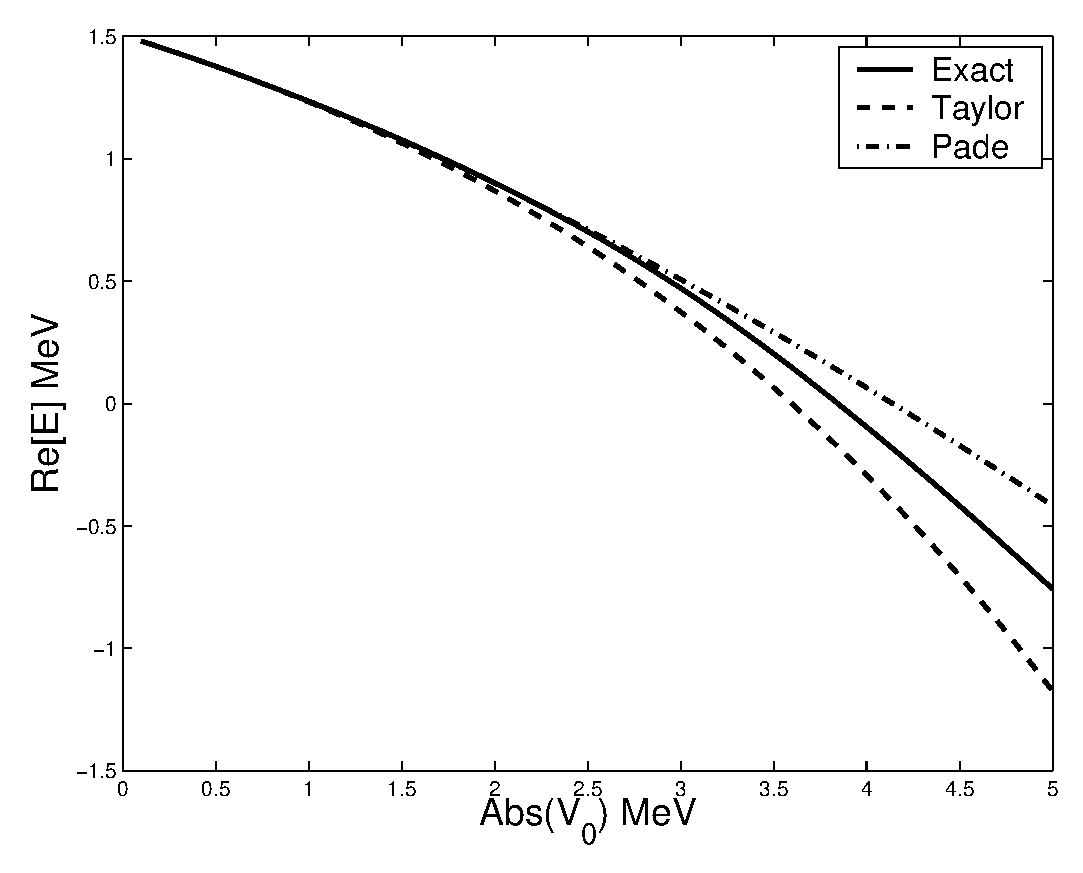
\epsfig{file=figures/pade_re.eps}}
\end{center}
\caption{Plot of real part of $0^+$ energy in $^6$He, for 
increasing interaction strength $V_0$. Solid line gives the exact energy, 
the dashed line gives the series expansion of the energy up through third
order and the dashed-dotted line gives the  $E^{[2,1]}$ Pade
approximation to the energy.} 
\label{fig:pade1}
\end{figure} 
Figure~\ref{fig:pade1} gives the real part of the $0^+$ energy, while 
figure~\ref{fig:pade2} gives the corresponding imaginary part of the energy, as the
interaction strength is gradually turned on. In both cases it is seen 
that the Pade approximant $E^{[2,1]}$ gives a better fit to the exact energy, than 
the Taylor expansion up through third order. In both cases the single-reference
perturbation theory fails to give satisfactory result for the energy when 
the interaction strength is that of Paper II, i.e. $V_0 = -5.315$MeV.  
\begin{figure}[hbtp]
\begin{center}
\resizebox{9cm}{7cm}{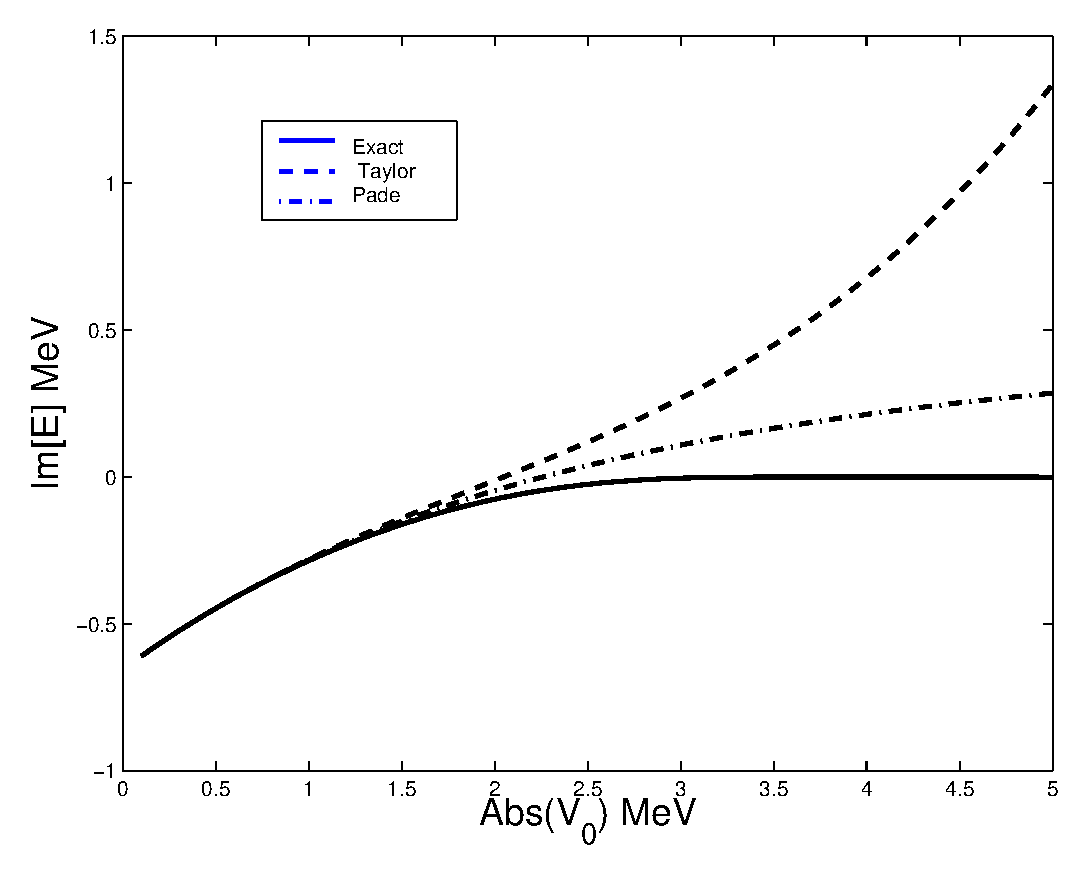
\epsfig{file=figures/pade_im.eps}}
\end{center}
\caption{Plot of imaginary part of $0^+$ energy in $^6$He, for 
increasing interaction strength $V_0$. Solid line gives the exact energy, 
the dashed line gives the series expansion of the energy up through third
order and the dashed-dotted line gives the  $E^{[2,1]}$ Pade
approximation to the energy.} 
\label{fig:pade2}
\end{figure} 
It is also seen that single-reference perturbation theory 
gives convergent results in this specific case only 
for interaction strengths less than $1$MeV. One may therefore
conclude that single-reference perturbation theory, is not
suitable in Gamow Shell Model calculations, since the coupling
with the complement space is too strong, for being treated perturbatively.

\subsection{Multi-reference perturbation theory.}
In this section we outline the non-Hermitian multi-reference perturbation theory.
We proceed in similar manner as in the previous section, and 
construct a $N$-body model space $P$ and 
a complement (orthogonal) space $Q$ according to equation~(\ref{eq:pq_op}). 
The choice of $P$ should 
be dictacted by some intuition on which single particle configurations 
play the dominant part in the fully correlated many-body wave function.
Having constructed $P$ and $Q$ the many-body wave function and the 
corresponding Hamiltonian may be represented in this basis. The Hamiltonian may 
subsequently be partioned into two parts according to, 
\begin{equation} 
  \left( \begin{array}{cc}
    PHP & PHQ \\ 
    QHP & QHQ  
  \end{array} \right)  =  
  \left( \begin{array}{cc}
    H^{PP} & 0 \\ 
    0 & H^{QQ}
  \end{array} \right) 
  +
  \left( \begin{array}{cc}
    0 & H^{PQ} \\ 
    H^{QP} & \tilde{H}^{QQ}  
  \end{array} \right) =  H_0 + H_1.
\end{equation}
Here $ D^{QQ}�$ is the diagonal part and $\tilde{H}^{QQ}�$ the off-diagonal part of $QHQ $ 
respectively. 
Written in this form, it is seen that $H^0$ defines the unperturbed part while $H^1$ gives the 
perturbations to $H^0$.  
Provided $H^0$ is non-singular, the model space block $PHP$ may be decoupled by   
constructing a complex orthogonal matrix $ {\bf C }��$ 
which diagonalizes  $H^0$, i.e. 
$ {\bf C}  H^0 {\bf C}^T = Diag(E^0_1, E_2^0,...,E_N^0) $. 
Since $H^0$ is  a block diagonal matrix, the matrix $ {\bf C }��$ is given in the form
\begin{equation}
  {\bf C} = \left[ \begin{array}{cc} 
      {\bf \chi } & {\bf 0} \\
	{\bf 0 }& {\bf 1 } 
    \end{array} \right]
\end{equation}
A more convienient many-body basis 
which decouples (diagonalizes) the reference space is then given by
\begin{equation}
  \Upsilon_i = \sum_{j=1}^N C_{i,j}\Phi_j = 
  \left\{ \begin{array}{c} \sum_{j=1}^{N_P}\chi_{i,j}\Phi_j ,\:\:  i = 1,N_P \\
    \Phi_i, \:\:\:\:\:\:\:\: i = N_P + 1, N 
  \end{array}\right. 
\end{equation}
and they are solutions of the eigenvalue problem,
\begin{equation}
  H_0  \vert \Upsilon_i \rangle = \tilde{\varepsilon}_i \vert \Upsilon_i \rangle.
\end{equation}
We assume here that the states $ \vert \Upsilon_i \rangle $ are normalized to unity.
The complex orthogonal matrix ${\bf \chi }$ which span the reference space $P$, 
defines our new set of reference states.  
The states $\Upsilon_i,\: i = 1,...,N_P�$ span the same space as
the original $P$-space states $\Phi_i$, but they have been reoriented in space
so that they diagonalize $PHP$.  
As a measure of how well the zeroth order wave 
function $\Upsilon_{i=\mathrm{res}}^J$ 
resembles the exact  wave function, one can calculate the complex variance 
$\sigma_c^2 $ see Refs.~\cite{nimrod,davidson3},
\begin{eqnarray} 
  \nonumber
  \sigma_c^2 & = & { \langle {\Upsilon_{i}^J}^* \vert 
    \left( H - E_{i}^0 \right)^2 \vert {\Upsilon}_{i}^J \rangle } \\
  & = & \chi^T_i H^{PQ}H^{QP} \chi_i, 
\end{eqnarray}  
where $i= \mathrm{res}$ and $ \chi_i $ labels the $i$'th column of the $N_P\times N_P$  matrix $\chi�$. 
In Ref.~\cite{davidson3}� it was proved that 
the complex variance $\sigma_c $ provides an upper bound to the exact resonance energy, 
\begin{equation}
  \left| E^{\mathrm{exact}}_{\mathrm{res}} - E_{\mathrm{res}}^0 \right| \leq \left| \sigma_c \right|
\end{equation} 
Having constructed a new many-body anti-symmetric basis, we develop 
a perturbation expansion in terms of these eigenvectors of the 
reference space. Derivation of the Rayleigh - Schr\"odinger perturbation
expansion for the exact energy and wave function follows in exactly the same manner
as in previous section. We wish to study how a single reference state $\Upsilon_i $ 
changes order by order in the Rayleigh-Schr\"odinger perturbation
expansion by adding the perturbation matrix $H^1$. So the 
$P$-space is a single state and the orthogonal complement is the remaining states
\begin{equation}
  \tilde{P} = \vert \Upsilon_a \rangle\langle \Upsilon_a^*\vert , \:\:
  \tilde{Q}�= \sum_{i\ne a}\vert \Upsilon_i \rangle\langle \Upsilon_i^*\vert.
\end{equation}
Consider the 1'st order correction to the energy
for any state $\Upsilon_p$ in the model space, i.e.
\begin{equation}
  E_1(p)  = \langle \Upsilon_p^* \vert H_1 \vert \Upsilon_p \rangle = 
  \left( \begin{array}{cc} \chi_p^{\mathrm{T}} &  0 \end{array}\right) 
  \left( \begin{array}{cc} 
    0 & H^{PQ} \\
    H^{QP} & H^{QQ} \end{array}\right) 
  \left( \begin{array}{c}
    \chi_p \\
    0 \end{array}\right)  = 0, 
\end{equation}
which gives zero contribution. This is an extremely nice feature, since
all expansion terms where 1'st order matrix elements $E_1$ appear in a product 
with more complicated terms give zero contribution. The 1'st order correction to the 
energy may be said to have been incorporated into the zeroth order energy 
$\tilde{\varepsilon}_i$.
The second order correction to an unperturbed energy $\tilde{\varepsilon}_p$
becomes
\begin{equation} 
E_2(p) =  \sum_{a\ne p}^N  {  \langle \Upsilon_p^* \vert H_1 
 \vert \Upsilon_a \rangle \langle \Upsilon_a^*\vert H_1 \vert \Upsilon_p \rangle 
\over \tilde{\varepsilon}_p -\tilde{\varepsilon}_a }
\end{equation}
from the structure of the perturbation matrix $H^1$ is easily seen that the sum over
$Q$-space states is restricted to $ a > N_P $ by taken into the account 
$ \langle \Upsilon_i^* \vert H_1 \vert \Upsilon_j \rangle = 0 ,\:\: i,j \leq N_P$.
This illustrates that many  excitations from the $P$- into the $Q$-space have
already been taken into account in the zeroth order wave function.
The second order energy term then becomes, 
\begin{eqnarray} 
  \nonumber E_2(p)&  = &   \sum_{a > N_P}^N  { \langle \Upsilon_p^* \vert H_1
    \vert \Upsilon_a \rangle \langle \Upsilon_a^*\vert 
H_1 \vert \Upsilon_p \rangle \over \tilde{\varepsilon}_p -\tilde{\varepsilon}_a }=
\sum_{i,j \le N_P } \sum_{a> N_P} { \chi_{p,i}
    \langle \Phi_i^*\vert H_1 \vert \Phi_a \rangle \langle \Phi_a^*\vert H_1 \vert \Phi_j\rangle \chi_{j,p} 
    \over  \tilde{\varepsilon}_p -\tilde{\varepsilon}_a }  \\
& = & \sum_{i,j \le N_P } \sum_{a> N_P} { \chi_{p,i}
  H^{PQ}_{i,a} H^{QP}_{a,j}\chi_{j,p} 
    \over  \tilde{\varepsilon}_p - D^{QQ}_{a,a} }. 
\end{eqnarray}
and the third order term becomes 
\begin{equation}
  E_3(p) =  \sum_{ \stackrel{a,b > N_P}{a \ne b}} ^N  �{ \langle \Upsilon_p^* \vert H_1 
  \vert \Upsilon_a \rangle \langle \Upsilon_b^* \vert H_1 \vert \Upsilon_p \rangle \over
  ( \tilde{\varepsilon}_p -\tilde{\varepsilon}_a) 
  ( \tilde{\varepsilon}_p -\tilde{\varepsilon}_b )�} 
  = \sum_{i,j \le N_P} \sum_{\stackrel{a,b > N_P}{a \ne b}} { \chi_{p,i} H^{PQ}_{i,a}\tilde{H}^{QQ}_{a,b}H^{QP}_{b,j}\chi_{j,p}
    \over   ( \tilde{\varepsilon}_p - D^{QQ}_{a,a}) 
    ( \tilde{\varepsilon}_p -D^{QQ}_{b,b} )�}. 
  \end{equation}
Higher order terms may easily calculated from the Rayleigh-Schr\"odinger perturbation
expansion given in equation(\ref{eq:rayleigh}).
Summarizing we get through fourth order, 
\begin{eqnarray}
  \nonumber E_0(p) &=& \langle \Upsilon_p^*\vert H^0 \vert \Upsilon_p \rangle = \tilde{\varepsilon}_p, \\
  \nonumber E_1(p) &=& \langle \Upsilon_p^*\vert H^1 \vert \Upsilon_p \rangle = 0, \\ 
  \nonumber E_2(p) &=& \langle \Upsilon_p^*\vert H^1 {Q\over \tilde{\varepsilon}_p - H^0} 
  H^1 \vert \Upsilon_p \rangle, \\
  E_3(p) &=& \langle \Upsilon_p^*\vert H^1 {Q\over \tilde{\varepsilon}_p - H^0} 
  H^1 {Q\over \tilde{\varepsilon}_p - H^0} H^1 \vert \Upsilon_p \rangle, \\
  \nonumber E_4(p) &=& \langle \Upsilon_p^*\vert H^1 {Q\over \tilde{\varepsilon}_p - H^0} 
  H^1 {Q\over \tilde{\varepsilon}_p - H^0} H^1 
  {Q\over \tilde{\varepsilon}_p - H^0} H^1 \vert \Upsilon_p \rangle \\
  \nonumber &-& E_2(p)\langle \Upsilon_p^* \vert H^1 {Q\over (\tilde{\varepsilon}_p - H^0)^2} 
  H^1 \vert \Upsilon_p \rangle. 
\end{eqnarray} 
Where $ Q = \sum_{i > N_P} \vert \Upsilon_i \rangle \langle \Upsilon_i ^*\vert $.

The above perturbation series is a theory which treats one-state-at-a-time, 
this theory differs from the standard multi-reference perturbation
theory which diagonalizes an effective Hamiltonian and solves for all 
states in the model space simultaneously. The above perturbation theory 
sets no restrictions on the choice of many-body reference space, and
can in principle be chosen by any suitable selection criterion. The 
theory also allows for a freely variation of the reference space size,
so that it is possible to achieve satisfactory convergent results 
at a given order in  the perturbation series. If the coupling between the 
reference states is turned off, the perturbation series reduces to the
standard single-reference Rayleigh-Schr\"odinger perturbation theory 
discussed in the previous section.

In the application of the above multi-reference perturbation theory 
method to Gamow Shell Model calculations, a reference space which 
takes into account most of the correlations has to be chosen. 
Further the size of the $P$-space should be small enough to allow
for a direct diagonalization in order to obtain the reference states 
$\Upsilon_i, \:\: i = 1,...,N_P$. The most important configuration in
a many-body resonance may be expected to be the pure resonance 
pole configuration  $\vert RRR...\rangle $. We wish then to 
generate correlations on this unperturbed many-body resonance 
state, in order to obtain the fully correlated many-body resonance.
The correlations are generated by virtual excitations of one or several
particles occupying the single particle resonant orbitals to non-resonant continuum 
orbitals, induced by the residual nucleon-nucleon interaction.
A viable starting point for Gamow Shell Model applications, would be
to construct a reference space $ P $ conisisting of a set of low lying 
many-body unperturbed states where at least one particle is in a single 
particle resonance orbital. The orthogonal complement  space $Q$ 
consits then of the remaining states. 
In Paper II where the above perturbation theory where applied to 
the unbound nucleus $^7$He, 
the three-particle model space, and corresponding complement space, 
where defined by
\begin{eqnarray}
  P \equiv 
  \left\{ \begin{array}{c} \vert RRR \rangle, \vert RRC\rangle, \vert RCC\rangle ,\\
    \mathrm{Re}(e_a+e_b+e_c) <  E_{\mathrm{cut}}, \\
    \mathrm{Im}(e_a+e_b+e_c) > -E_{\mathrm{cut}}
  \end{array} \right\}\:\:\: Q = 1-P,
  \label{eq:mspace1}
\end{eqnarray}
here the $P$ space is given by configurations where at most two 
particles move in continuum orbits. In addition, $P$ is further defined by a
rectangular cutoff in the complex energy plane. This cutoff in energy is motivated by 
an assumption that three-particle configurations high in 
energy play a minor role on the formation of low-lying resonances.
Figure~\ref{fig:P_space_ch1} gives a plot of the $J^\pi = {3/2}^-$ 
unperturbed (non-interacting) 
three-particle spectrum of $^7$He used in Paper II.  
At most two particles move in complex continuum orbits, 
and three different cut-offs in energies and corresponding model spaces are shown. 
Note that only $p_{3/2} $ single particle orbitals are taken into account.
\begin{figure}[hbtp]
\begin{center}
\resizebox{9cm}{7cm}{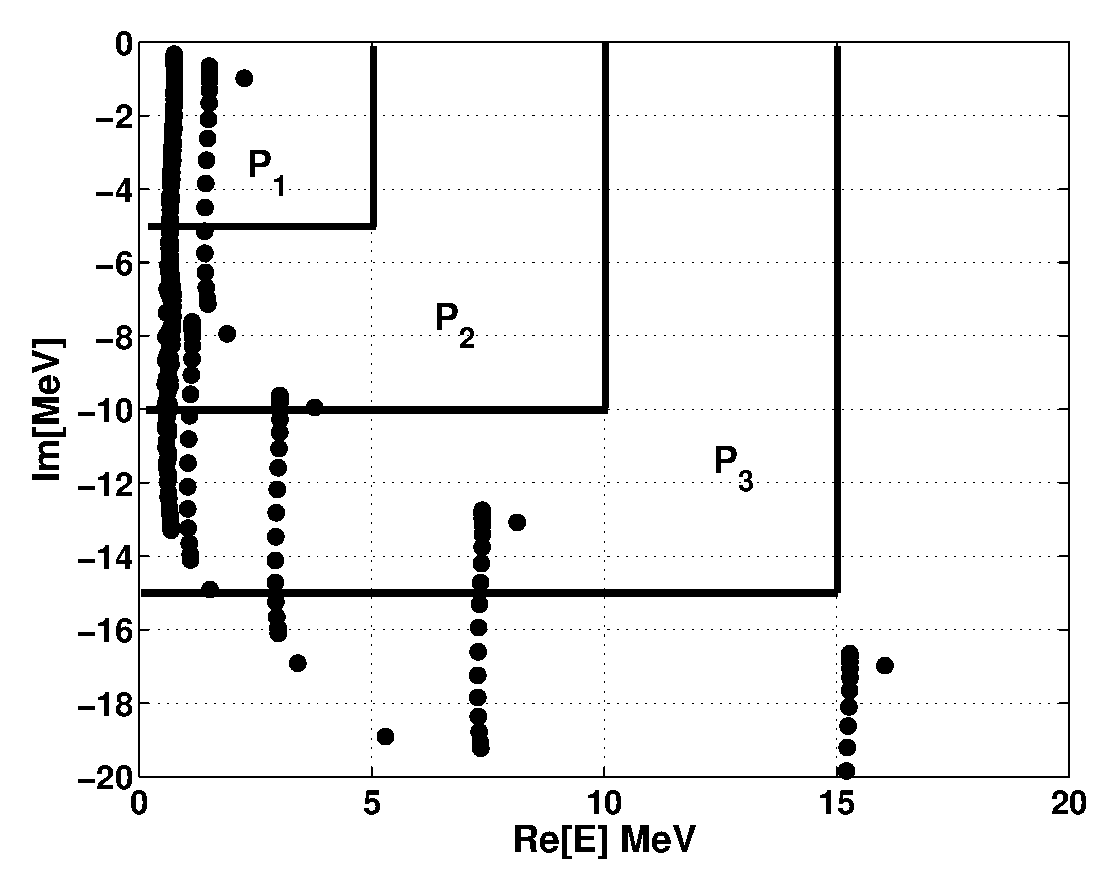
\epsfig{file=figures/fig10.eps}}
\end{center}
\caption{Three choices of the model space used in the multi-configuration 
perturbation method. The three-particle model space states are constructed
such that at most two particles move in the non-resonant continuum.} 
\label{fig:P_space_ch1}
\end{figure} 
Having constructed a suitable model space $P$, a full diagonalization
is performed. We wish to study the effect of adding the perturbation $H^1 $
to the new many-body resonance wave function. Since the above theory 
is one-state-at-a-time theory, the zeroth order resonance $ \Upsilon (i=res) $
has to be identified from the zeroth order energy spectrum.  This identification may 
may be done by determining which state $ \Upsilon_i, \:\: i = 1, ...,N_P $ has the 
largest overlap with the pure pole configuration 
$\vert \Phi_{\mathrm{res}}\rangle �= \vert RRR... \rangle $,
\begin{equation}
  \mathrm{Max} \left\{ \left|�\langle  \tilde{\Phi}(\mathrm{res}) \vert 
  \Upsilon_i  \rangle \right| \right\}_{i=1}^{N_P}=
  \mathrm{Max} \left\{ \left|�\chi_{i,j={\mathrm{res}} } \right| \right\}_{i=1}^{N_P}
  \label{eq:overlap}
\end{equation}
To make sure the ``correct'' physical state is picked out, the
complex energy trajectories as the interaction is gradually turned on may 
be studied. 
 
% new section
\section{Effective interaction scheme for Gamow shell model calculations}
\label{sec:effective_scheme}

In the previous sections it was shown that the Lee-Suzuki similarity transformation 
and the multi-reference perturbation method may be used in the Gamow shell model 
in order to  account for the most important correlations of for example a  multi-particle resonance. 
Although the dimensionality of the problem derived either 
from the similarity transformation method or the multi-reference perturbation method 
was significantly reduced compared to the full problem, the dimensionality may still be a severe
problem when dealing with more than three particles in a big valence space. 

The drawback of the multi-reference perturbation method is that one has to store 
extremely large matrices $H^{QQ}$ 
if one wishes to go beyond second order in perturbation theory. In the similarity 
transformation method one does not have to deal with $H^{QQ}$, as couplings with
the $Q$-space states have been dealt with, in practical calculations at least at the two-body level. 
Going to systems with larger degrees of freedom, the $P$-space may nevertheless,
at the converged level, be too large for our brute force diagonalization approach.

The aim of this section is to propose an effective interaction and perturbation theory scheme 
for the Gamow shell model. This approach 
combines the similarity transformation method and the multi-reference perturbation method,
so that hopefully multi-particle resonances where several particles move 
in large valence spaces, may be calculated without a diagonalization in the full space.
Our algorithm is as follows
\begin{enumerate}
\item Choose an optimal set of $n_{sp}$ single-particle orbits, which in turn defines 
two-body  $P_{2p}$ and  many-body spaces. In our case  these single-particle orbits are defined by 
selected states in $^5$He.
\item Construct a two-particle effective interaction by the Lee-Suzuki similarity transformation method
  within the two-particle model space $P_{2p}$. Such diagonalizations can be done for very large spaces,
see for example Refs.~\cite{bruce1,bruce2,bruce3,bruce4}.
\item The next step is to divide the multi-particle model space $P$ in two smaller spaces $P'$ and $Q'$, 
  where $P=P'+Q'$ and $ N_P = N_{P'} +N_{Q'}  $. 
  The choice of $P'$ should be dictated by our knowledge of the physical system. As an example, 
one may consider those single-particle configurations within the $P-$space that play 
the dominant role in the formation of 
  the multi-particle resonance.  The number $N_P = N_{P'} + N_{Q'}$ represents the total number of 
  many-body configurations within the $P-$space.
\item Now that we have divided the $P$-space in two sub-spaces $P'$ and $Q'$, we use for example 
  the multi-reference perturbation method  to account for 
  excitations from the $P'-$ space to the $Q'-$ space to obtain energy corrections to a specific order.
  Increase the size of the $P'-$space until convergence is obtained. In the case $N_{P'} = N_P $ and 
  $N_{Q'} = N_P-N_{P'} = 0$ the multi-reference perturbation expansion terminates at zeroth order,
  and corresponds to a full diagonalization within the $P-$space. 
  Another option is to use for example the coupled cluster method as exposed in Refs.~\cite{cc1,cc2}. 
\item Start from top again with a larger set of single-particle orbits, 
  and continue until a  convergence criterion is reached.
\end{enumerate}
We illustrate these various choices of model spaces in the following two figures.
figure~\ref{fig:paulioperator} defines our model space for the Lee-Suzuki similarity transformation
at the two-body level. This corresponds to steps one and two in the above algorithm.
The set of single-particle orbits defines the last single-particle orbit in the model space $n_{sp}$. 
Note that we could have chosen a model space defined by a cut in  energy, as done by the No-Core
collaboration, see for example Refs.~\cite{bruce1,bruce2,bruce3,bruce4}. These examples serve just to 
illustrate the algorithm.
\begin{figure}[htb]
\begin{minipage}[t]{80mm}
%\framebox[79mm]{\rule[-26mm]{0mm}{52mm}}
\setlength{\unitlength}{0.6cm}
\begin{picture}(9,10)
\thicklines
   \put(1,0.5){\makebox(0,0)[bl]{
              \put(0,1){\vector(1,0){8}}
              \put(0,1){\vector(0,1){8}}
              \put(-0.6,6){\makebox(0,0){$n_{sp}$}}
              \put(5,0.5){\makebox(0,0){$n_{sp}$}}
              \put(2,3){\makebox(0,0){$\hspace{1cm}P_{2p}$}}
              \put(2,7){\makebox(0,0){$\hspace{1cm}Q_{2p}=1-P_{2p}$}}
              \put(0,6){\line(1,0){5}}
              \put(5,1){\line(0,1){5}}
         }}
\end{picture}
\caption{Possible definition of the two-body 
exclusion operator $Q_{2p}=1-P_{2p}$ used to compute the 
Lee-Suzuki similarity transformation and its effective interaction at the two-body level. 
The border of the model space is defined by the last single-particle orbit $n_{sp}$. 
\label{fig:paulioperator}}
\end{minipage}
%
\hspace{\fill}
%
\begin{minipage}[t]{75mm}
%\framebox[74mm]{\rule[-26mm]{0mm}{52mm}}
\setlength{\unitlength}{0.6cm}
\begin{picture}(9,10)
\thicklines
   \put(1,0.5){\makebox(0,0)[bl]{
              \put(0,1){\vector(1,0){8}}
              \put(0,1){\vector(0,1){8}}
              \put(-0.6,6){\makebox(0,0){$N_P$}}
              \put(5,0.5){\makebox(0,0){$N_P$}}
              \put(-0.6,3){\makebox(0,0){$N_{P'}$}}
              \put(2,0.5){\makebox(0,0){$N_{P'}$}}
              \put(0,6){\line(1,0){5}}
              \put(5,1){\line(0,1){5}}
              \put(0,3){\line(1,0){2}}
              \put(2,1){\line(0,1){2}}
         }}
\end{picture}
\caption{Possible definition of many-body space $N_P$ and reduced space $N_P'$. \label{fig:finalp}}
\end{minipage}
\end{figure}
Figure~\ref{fig:finalp} demonstrates again a possible division of the three- and many particle space 
into the full model space
$P$ and a smaller space ${P'}$. Again, this 
figure serves only the purpose of illustrating the method.
In our actual calculations we define the smaller space ${P'}$ via an energy cut in the real and 
imaginary eigenvalues and selected many-body configurations.
 
In summary, defining a set of single-particle orbits in order to construct the two-body and many-body 
model spaces, we obtain first an effective two-body interaction in the  space $P_{2p}$
by performing the 
Lee-Suzuki \cite{suzuki1,suzuki2,suzuki3,suzuki4} transformation. This interaction and the 
pertinent single-particle orbits are then used to define a large many-body space. 
It is therefore of interest to see if we can reduce this dimensionality through the definition of smaller
spaces and perturbative corrections. 

\section{Inclusion of realistic nucleon-nucleon interactions in Gamow
  shell model calculations}
\label{sec:realistic_interactions}
In microscopic nuclear many-body calculations, the strong 
short range repulsion in realistic nucleon-nucleon interactions 
complicates the calculations considerably since the repulsive core 
makes a perturbative treatment unsuitable. Therefore we wish
to construct a renormalized interaction in a  model space, which 
smoothes out the repulsive core of the bare nucleon-nucleon interaction.
Typically, the renormalized nucleon-nucleon interaction has been constructed
from the Brueckner G-matrix approach (see Ref.~\cite{mhjensen}). The G-matrix 
is a soft interaction, which is obtained by resumming in-medium particle-particle
scattering. The renormalized G-matrix is both energy- and nucleus dependent, which 
makes it difficult to extend the G-matrix to drip line nuclei.
Recently, an alternative approach, to the renormalized G-matrix,
which integrates out the high momentum components of the nucleon-nucleon
interactions has been proposed \cite{bogner,fujii,fujii2,nogga}. 
Using a similarity transformation of the two-nucleon Hamiltonian,
a Hermitian soft-core effective nucleon-nucleon interaction is obtained
in a model model space defined by a cutoff $\Lambda �$ in relative momentum
between the nucleons. This effective interaction has become known, as
a low-momentum nucleon-nucleon (LMNN) interaction, $V_{\mathrm{low-k}}$. 
The $V_{\mathrm{low-k}}$ is an energy and nucleus indepedent effective interaction, 
which depends only the model space cutoff $\Lambda $ and the 
bare nucleon-nucleon interaction. 
The effective low-momentum interaction ($V_{\mathrm{low-k}}$)
is constructed in such a way that it reproduces 
exactly the main characteristics of the 
nucleon-nucleon wave function in the full space. 
The $V_{\mathrm{low-k}}$ is a promising approach for 
nuclei along the drip lines. 

In this section, we show that it is possible 
to obtain a $V_{\mathrm{low-k}}$ in the complex $k$-plane, 
starting with the momentum space Schr\"odinger equation 
defined on an inversion symmetric contour $L^+$. As an illustration we construct 
a $V_{\mathrm{low-k}}$ on a purely rotated contour using the realistic CD-Bonn 
nucleon-nucleon interaction \cite{machleidt}. The effective interaction 
may then be the basic input in microscopic calculations of many-body 
resonances. In the following we outline the procedure for obtaining a complex symmetric
$V_{\mathrm{low-k}}$, based on the Lee-Suzuki similarity transformation for complex
interactions (see Section~\ref{sec:lee_suzuki}) and the Contour Deformation Method 
(see Section~\ref{sec:analytic_continuation}).
Starting with the transformed momentum space Schr\"odinger equation, 
\begin{equation}
  \int_{L^+}dk'\:{k'}^2 \langle k^*\vert T + V \vert k'\rangle \langle {k'}^*\vert \psi_{n}\rangle
  = E_{n} \langle k^*\vert \psi_{n}\rangle. 
\end{equation}
where the plane wave states are eigenfunctions of the kinetic energy 
operator and they form a complete set 
\begin{equation}
  \int_{L^+} dk \:k^2 \vert k\rangle \langle k^*\vert. 
\end{equation}
The momentum space Schr\"odinger equation is solved as a matrix equation
by discretizing the integration contour $L^+$ by some suitable 
quadrature rule, e.g. Gauss-Legendre quadrature. The discretized Schr\"odinger equation
becomes on the chosen contour 
\begin{equation}
  \sum_j w_j k_j^2 \langle k_i^*\vert T+V\vert k_j \rangle \langle k_j^*\vert\psi_{n}\rangle 
  =  E_{n} \langle k_i^*\vert \psi_{n}\rangle. 
  \label{eq:vlowk1}
\end{equation}
Here $k_i$ are the integration points and $w_i$ the corresponding quadrature weights.
Introducing the modified plane wave kets
$\vert \bar{k_i} \rangle�= k_i\sqrt{w_i}�\vert k_i \rangle $, equation~(\ref{eq:vlowk1}) 
becomes
\begin{equation}
  \sum_j  \langle \bar{k_i}^*\vert T+V \vert \bar{k_j} \rangle 
  \langle \bar{k_j}^*\vert\psi_{n}\rangle 
  =  E_{n} \langle \bar{k_i}^*\vert\psi_{n}\rangle. 
  \label{eq:vlowk2}
\end{equation}
where we have 
\begin{equation}
  1 = \sum_{i=1}^N \vert \bar{k_i} \rangle\langle \bar{k_i}^*\vert, \:\:
  \langle \bar{k_i}^*\vert \bar{k_j} \rangle = \delta_{i,j}.
\end{equation}
The matrix elements of the Hamiltonian becomes in the plane wave basis
\begin{equation}
  H_{i,j} = \langle \bar{k_i}^*\vert T+V \vert \bar{k_j} \rangle  = 
  {k_i^2\over 2\mu}\delta_{i,j} + \sqrt{w_iw_j}k_ik_j V_l(k_i,k_j).
\end{equation} 
The full space is now divided in a model space $P$ and an orthogonal complement 
space $Q$. The model space $P$ consits of the $N_P$  plane wave states
lying below some cutoff $\Lambda $ in momentum, and the $Q$-space
consists of the remaining states, i.e.
\begin{equation}
  P = \left\{ \vert \bar{k_p}\rangle, \:\: \vert k\vert  \leq \Lambda \right\}, \:\:
  Q = \left\{ \vert \bar{k_q}\rangle, \:\: \Lambda < \vert k\vert < \infty \right\}.
\end{equation}
In order to obtain an effective interaction in the model space $P$,
the decoupling condition in equation~(\ref{eq:decoup}) 
has to be fulfilled and we have to solve
for the transformation operator $\omega$ in equation~(\ref{eq:omega}).
Given the transformation matrix $\omega $ in the plane wave basis
$ \langle \bar{k}^*_q \vert \: \omega \: \vert \bar{k}_p \rangle $, the
low-momentum effective nucleon-nucleon interaction $V_{\mathrm{low-k}}$, 
of the Okubo form (equation~(\ref{eq:okubo})) is given by 
\begin{eqnarray}
  \nonumber \langle \bar{k_p}^*\vert V_{\mathrm{low-k}} \vert \bar{k_p}'\rangle & = & 
  \sum_{k_p''}\sum_{k_p'''}
  \langle \bar{k_p}^* \vert (P+\omega^{\mathrm{T}}\omega )^{1/2} \vert \bar{k_p}'' \rangle
  \langle \bar{k_p}''^* \vert H_{LS} \vert \bar{k_p}'''\rangle 
  \langle \bar{k_p}'''^*\vert  (P+\omega^{\mathrm{T}}\omega )^{-1/2} \vert \bar{k_p}'\rangle \\
  & - & {k_p^2\over 2\mu} \delta_{k_p,k_p'},
\end{eqnarray} 
see Section~\ref{sec:lee_suzuki} for further details. The effective interaction 
in the original plane wave basis $\vert k_i \rangle $ is then given by 
\begin{equation}
  \nonumber \langle {k_i}^*\vert V_{\mathrm{low-k}} \vert {k_j}'\rangle  =  
  { \nonumber \langle \bar{k_i}^*\vert V_{\mathrm{low-k}} \vert \bar{k_j}'\rangle 
    \over \sqrt{w_iw_j} k_ik_j },
\end{equation}
where $\left\{ \vert k_i\rangle, \:\vert k_j \rangle\right\}  \in P$.

The aim is to obtain a realistic effective nucleon-nucleon interaction, 
which is applicable in microscopic calculations of many-body 
resonances, which takes the continuum properly into account.
As discussed in detail in the previous sections, the nucleon-nucleon
interaction has to be analytically continued onto the second 
energy sheet, in order to obtain resonances in the calculated spectrum.
From a CDM perspective, 
we wish then to obtain a low-momentum nucleon-nucleon interaction, $V_{\mathrm{low-k}}$,
on an inversion symmetric contour in the complex $k$-plane. Here we 
illustrate how this may be achieved for the realistic CD-Bonn \cite{machleidt} 
interaction. A constraint on the theory, is that all low-energy characteristics
of the nucleon-nucleon system are conserved. We consider a contour $L^+$�of 
the simplest kind, which is just a purely rotated contour in the $k$-plane.
See figure~\ref{fig:contour1} for an illustration of the contour. 
\begin{figure}[hbtp]
\begin{center}
\resizebox{11cm}{7cm}{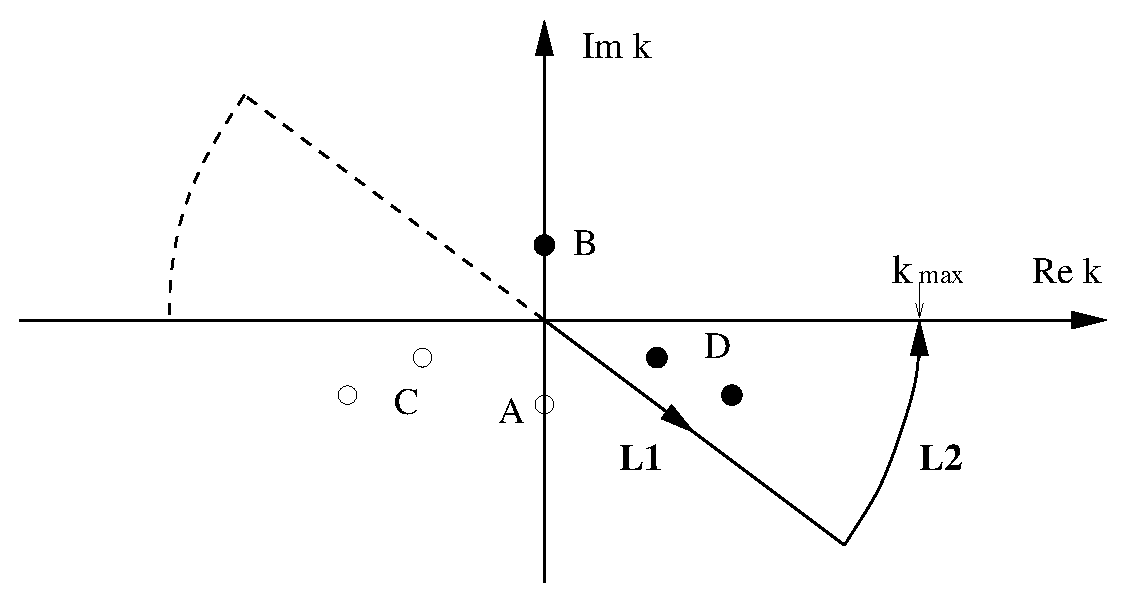
\epsfig{file=figures/fig2.eps}}
\end{center}
\caption{Contour $ L^{+} = L_{1} + L_{2} $ is given by the solid line, while
the contour $L^{-} $ is given by the dashed line. The contour $L= L^{+}+L^{-}$ is clearly
\emph{inversion symmetric}. The two body spectrum which is exposed by this contour is marked by 
filled circles $ \bullet $ and the excluded spectrum by open circles $\circ $.
 The full spectrum includes bound states (B), 
antibound (A), decay (D) and capture (C) resonant states.}
\label{fig:contour1}
\end{figure}

\begin{figure}[hbtp]
\begin{center}
\resizebox{11cm}{10cm}{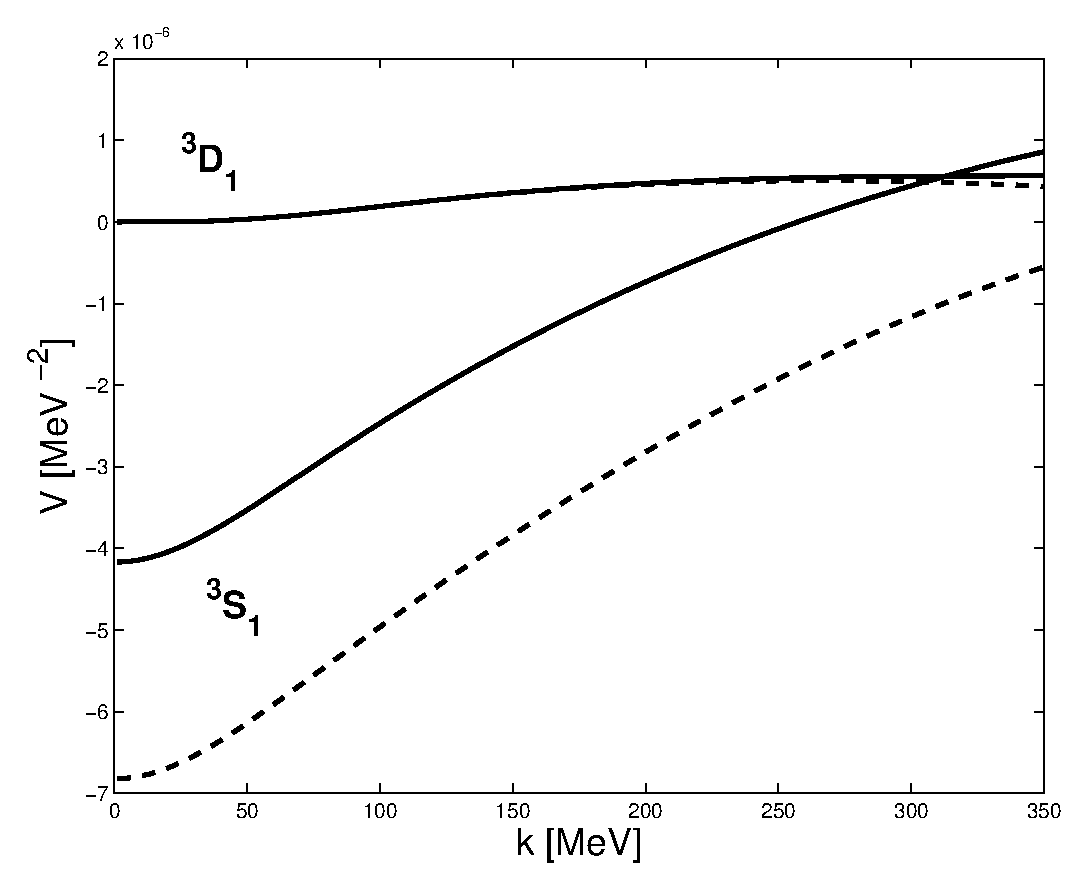
\epsfig{file=figures/vlowk1.eps}}
\end{center}
\caption{Plot of the real  part  of the 
  non-scaled $\theta = 0 $ low-momentum nucleon-nucleon interaction for 
  a model space cutoff $ \Lambda = 2 \hbar c$MeV. Here the diagonal part of 
  the interaction for the deuteron channel $^3S_1 - ^3D_1 $ is shown.
  In the plot the momentum $k$ is
  given in MeV.}
\label{fig:vlowk1}
\end{figure}
The momentum space Schr\"odinger equation for the low momentum nucleon-nucleon
interaction becomes on the rotated contour $L^+_\Lambda \equiv \exp(-i\theta) \vert k\vert, \:
\vert k \vert \leq \Lambda$, 
\begin{equation}
  \int_{0}^{\vert k'\vert = \Lambda} d k' \: {k'}^2 \langle k^*\vert T + V_{\mathrm{low-k}} 
  \vert k'\rangle \langle {k'}^*\vert \psi_{n}\rangle
  = E_{n} \langle k^*\vert \psi_{n}\rangle, 
\end{equation}
with $k= \exp(-i\theta)\vert k \vert $. Discretizing the contour defined from 
$ \vert k \vert = 0$ to $\vert k\vert = \Lambda$, the matrix 
equation is obtained 
\begin{equation}
  \sum_j  \langle \bar{k_i}^*\vert T+V_{\mathrm{low-k}} \vert \bar{k_j} \rangle 
  \langle \bar{k_j}^*\vert\psi_{n}\rangle 
  =  E_{n} \langle \bar{k_i}^*\vert\psi_{n}\rangle. 
  \label{eq:vlowk3}
\end{equation}
with the matrix elements of the Hamiltonian given by
\begin{equation}
  H_{i,j} = \langle \bar{k_i}^*\vert T+V_{\mathrm{low-k}} \vert \bar{k_j} \rangle  = 
  {k_i^2\over 2\mu}\delta_{i,j} + \sqrt{w_iw_j}k_ik_j V_{\mathrm{low-k}}(k_i,k_j).
\end{equation} 
A two-dimensional interpolation routine is used 
in order to obtain $V_{\mathrm{low-k}}$ at arbitrary points on the 
contour $L^+_\Lambda$.
Figure~\ref{fig:vlowk1} gives a plot of the diagonal part of
the  $V_{\mathrm{low-k}}$ ( dashed line )
interaction and the original CD-Bonn (solid line) nucleon-nucleon interaction 
for the deuteron channel $^3S_1-^3D_1$, for the non-scaled case ($\theta = 0$).
In Refs.~\cite{fujii,bogner} it was shown that the binding energy of the deuteron 
and the scattering phase shifts below $E_{\mathrm{lab}} < 300 $MeV 
using $V_{\mathrm{low-k}} $ for a model space cutoff�$\Lambda = 2 \mathrm{fm}^{-1}$,
reproduce exactly the ones obtained from the original nucleon-nucleon interaction. 
This is only to be expected since a similarity transformation of the
Hamiltonian does not change the energies. 
However, it was shown in Ref.~\cite{fujii} the $D$-state probability of the deuteron
is not reproduced for momentum cutoffs smaller than $ \Lambda \sim 4-5\mathrm{fm}^{-1}$, 
see also table~\ref{tab:vlowk1} for the non-scaled case $\theta =0$.
The exact value of the $D$-state probability is retained for these values of�$\Lambda$, 
by using the corresponding 
similarity transformed projection operator onto the $D$-state. 
In Ref.~\cite{fujii} the application of $V_{\mathrm{low-k}}$ in 
calculation of the binding energy of the nuclei $^3 \mathrm{H}, ^4$He and 
$^{16}$O 
where studied. It was found, in comparison with exact calculations 
using the bare nucleon-nucleon interaction, that a satisfactory convergence 
for the binding energies where obtained for a momentum cutoff 
$ \lambda \geq 5\mathrm{fm}^{-1}$. In addition  the convergence
of the single particle energies in $^{16}$O where studied,
and also here a satisfactory convergence where obtained for 
$\Lambda \geq 5\mathrm{fm}^{-1}$. 

In table~\ref{tab:vlowk1} we show results for the deuteron binding energy and 
the $D$-state probability for different cutoffs $\Lambda $, 
for the non-scaled case ($\theta = 0$) and the complex scaled case $(\theta = \pi/6$).
The deuteron binding energy is reproduced for all cutoffs, as expected. 
It is seen that the $D$-state probability, for the non-scaled case ($\theta = 0$), 
decreases monotonically for smaller and smaller cutoff $\Lambda$. 
The $D-state$ probability saturates at the exact value for a 
cutoff $ \Lambda \sim 5\mathrm{fm}^{-1}$, this is consistent with the findings
in Refs.~\cite{fujii,fujii2,nogga} where the ground state energy of the considered 
nuclei $^3 \mathrm{H}, ^4$He and $^{16}$O are converged for a cutoff 
$\Lambda \geq 5\mathrm{fm}^{-1}$. 

It is also seen for the complex scaled case ($\theta = \pi/6$)
that the deuteron binding energy is reproduced at all values 
of $\Lambda$. Further it is observed that 
the $D$-state probability saturates at the exact value 
even slower than in the non-scaled case. It is seen that for 
$\lambda < 5 \mathrm{fm}^{-1}$ the $D$-state probability 
aquires in addition to the real part, a considerable imaginary part.
In this case a satisfactory converged $D$-state probability is obtained 
for a cutoff $\Lambda \geq 7 \mathrm{fm}^{-1}$.  This gives an indication
of the cutoff $\Lambda $ required to give converged results in nuclear 
structure calculations, using complex scaled low-momentum nucleon-nucleon  
interactions.
\begin{table}[htbp]
  \begin{center}
  \begin{tabular}{cccccccc}
    \hline 
    \multicolumn{1}{c}{ } & \multicolumn{3}{c}{$\theta = 0 $} 
    & \multicolumn{4}{c}{$\theta = \pi/6 $} \\
    \hline
    \multicolumn{1}{c}{$\Lambda$fm$^{-1}$ } & \multicolumn{1}{c}{Re$[E_{\mathrm{d}}]$} 
    & \multicolumn{1}{c}{Im$[E_{\mathrm{d}}]$} 
    & \multicolumn{1}{c}{$P_D(\%)$} 
    & \multicolumn{1}{c}{Re$[E_{\mathrm{d}}]$} 
    & \multicolumn{1}{c}{Im$[E_{\mathrm{d}}]$} 
    & \multicolumn{1}{c}{Re($P_D(\%)$)} 
    & \multicolumn{1}{c}{Im($P_D(\%)$)} \\ 
    \hline
    1. & -2.2246 & 0. &  1.22 & -2.2246 & -1.5E-05 & 0.64 & -1.39 \\
    2. & -2.2246 & 0. &  3.56 & -2.2246 & -1.5E-05 & 4.05 & -2.11 \\
    3. & -2.2246 & 0. &  4.56 & -2.2246 & -1.6E-05 & 5.41 & -0.58 \\ 
    4. & -2.2246 & 0. &  4.81 & -2.2246 & -1.1E-05 & 5.05 & 8.E-02  \\
    5. & -2.2246 & 0. &  4.85 & -2.2246 & -3.1E-05 & 4.86 & 6.E-02 \\
    6. & -2.2246 & 0. &  4.85 & -2.2246 & -1.5E-05 & 4.84 & 2.E-02 \\ 
    7. & -2.2246 & 0. &  4.85 & -2.2246 & -1.5E-05 & 4.85 & -8.E-05 \\ 
    8. & -2.2246 & 0. &  4.85 & -2.2246 & -1.5E-05 & 4.85 & -3.E-03 \\ 
    9. & -2.2246 & 0. &  4.85 & -2.2246 & -1.7E-05 & 4.85 & -2.E-03 \\ 
    \hline
    Ref.~\cite{machleidt} & -2.2246 & 0. & 4.85 & {} & {}  & {}  & {} \\ 
    \hline
  \end{tabular}
  \caption{Deuteron binding energy (in MeV) as function of cutoff $\Lambda $ (in fm$^{-1}$), 
    and
    $D$-state probability $P_D(\%)$. The non-scaled $\theta = 0$ 
    and complex scaled $\theta = \pi/6$ 
    Hamiltonians are considered.}
  \label{tab:vlowk1}
  \end{center}
\end{table}
 

\begin{figure}[hbtp]
\begin{center}
\resizebox{18cm}{9cm}{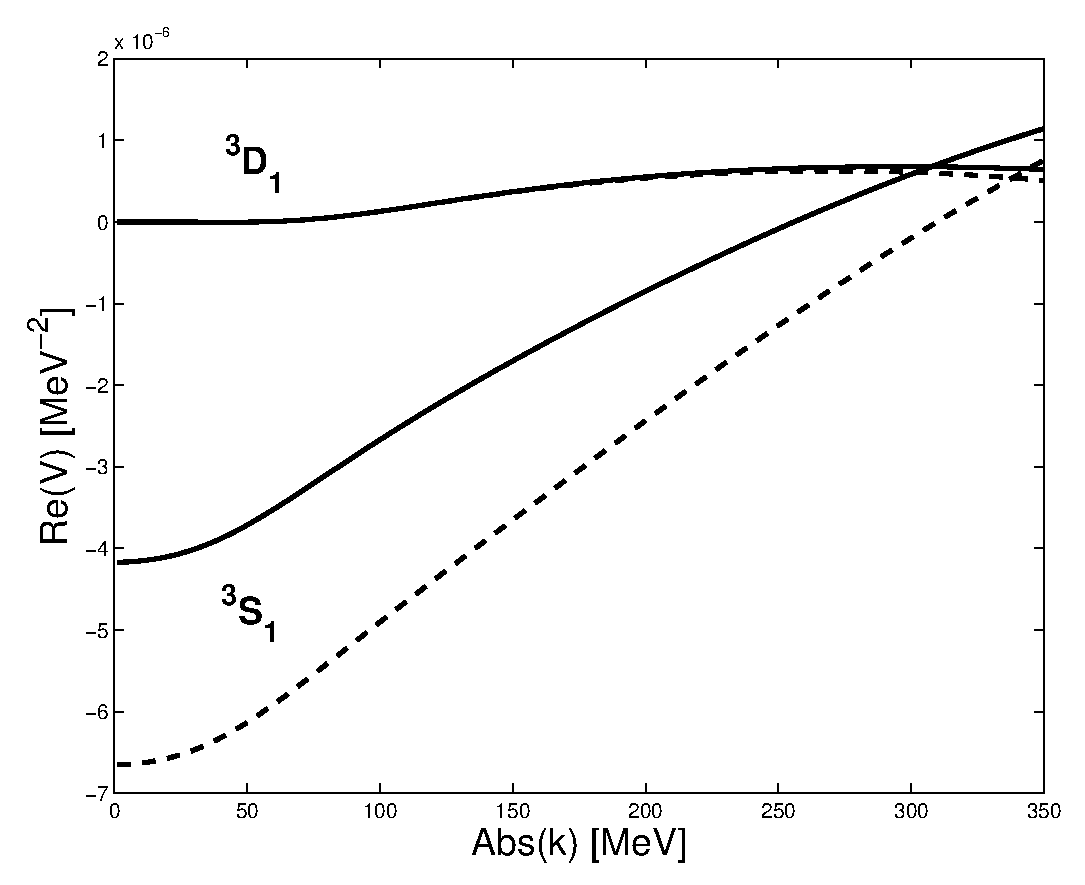
\epsfig{file=figures/vlowk_re.eps},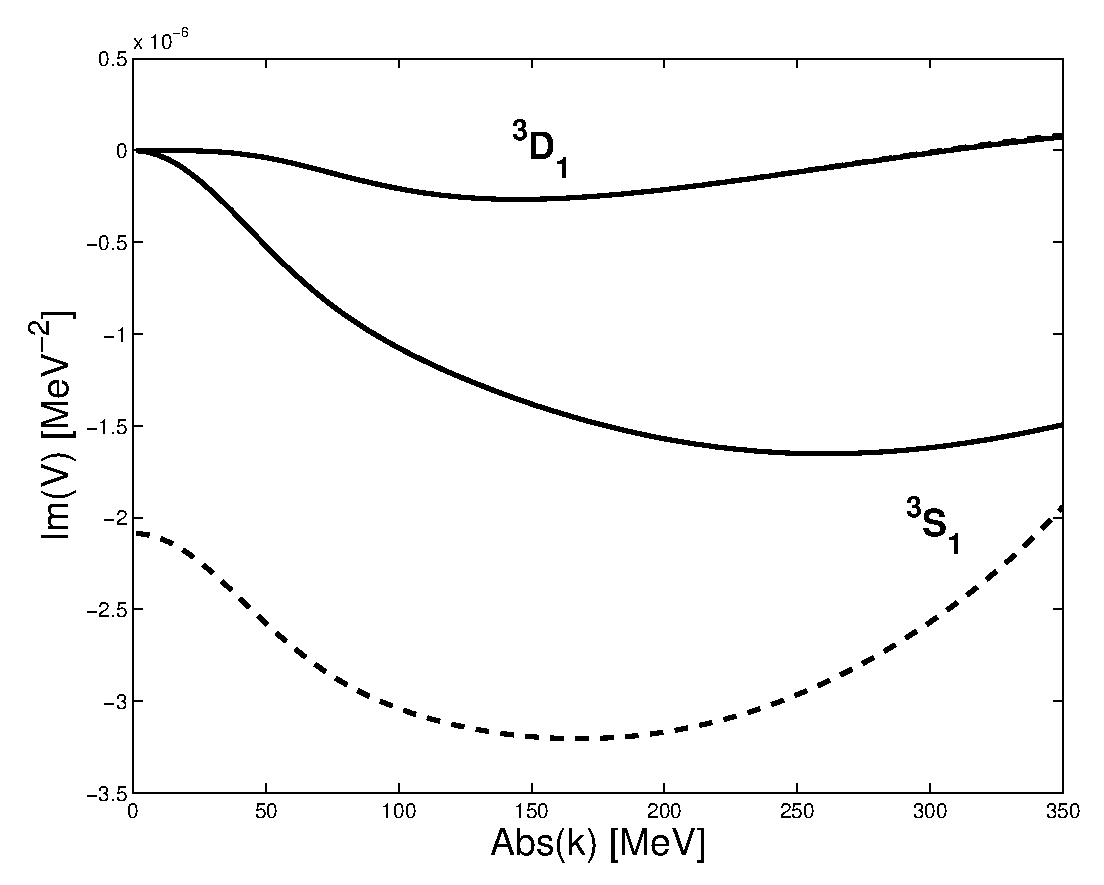
\epsfig{file=figures/vlowk_im.eps}}
\end{center}
\caption{Plot of the real (left plot) and imaginary (right plot) part  of the 
  complex scaled $\theta = \pi/6 $ low-momentum nucleon-nucleon interaction for 
  a model space cutoff $ \Lambda = 2 \mathrm{fm}^{-1}$. Here the diagonal part of 
  the interaction for the deuteron channel $^3S_1 - ^3D_1 $ is shown.
  In the plot the momentum $k$ is
  given in MeV.}
\label{fig:vlowk_re1}
\end{figure}
Figure~\ref{fig:vlowk_re1} gives a plot of the real (left plot) and imaginary (right plot)
parts of the diagonal part of the complex scaled $V_{\mathrm{low-k}}$ for deueteron channel, 
using a cutoff $\Lambda = 2\mathrm{fm}^{-1}$. It is seen that the imaginary part
of $V_{\mathrm{low-k}}$ is far from zero at $k=0\mathrm{fm}^{-1}$, 
which imply that the imaginary part
of the effective potential in this case does not solely originate from the complex scaled
momenta $k$. The unphysical imaginary part which occur for the $D$-state probability at 
$\Lambda = 2\mathrm{fm}^{-1}$  may therefore traced back to the non-zero imaginary part of
$V_{\mathrm{low-k}}$ at $k=0 \mathrm{fm}^{-1}$.
\begin{figure}[hbtp]
\begin{center}
\resizebox{18cm}{9cm}{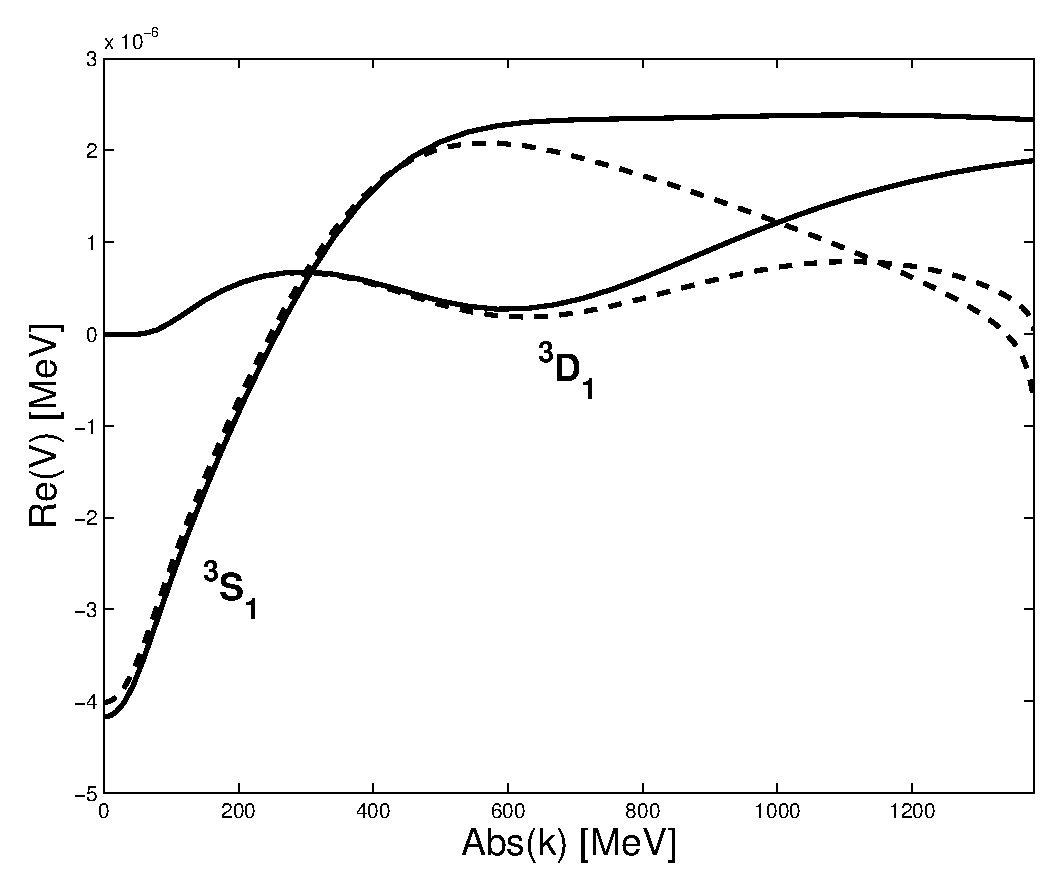
\epsfig{file=figures/vlowk_re2.eps},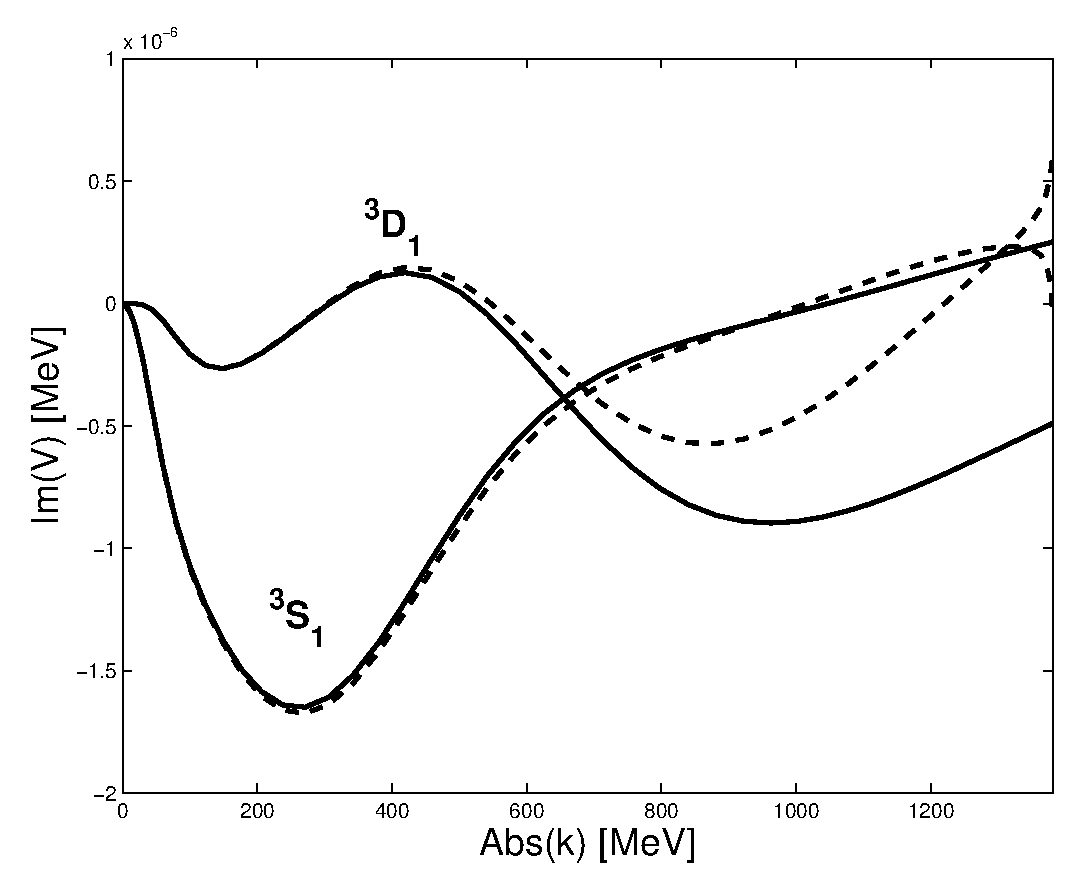
\epsfig{file=figures/vlowk_im2.eps}}
\end{center}
\caption{Plot of the real (left plot) and imaginary (right plot) parts of the 
  complex scaled $\theta = \pi/6 $ low-momentum nucleon-nucleon interaction for 
  a model space cutoff $ \Lambda = 7 \mathrm{fm}^{-1}$. Here the diagonal part of 
  the interaction for the deuteron channel $^3S_1 - ^3D_1 $ is shown.
  In the plot the momentum $k$ is
  given in MeV.}
\label{fig:vlowk_re2}
\end{figure}
Figure~\ref{fig:vlowk_re2} gives a plot of the real (left plot) and imaginary (right plot)
parts of the diagonal part of the complex scaled $V_{\mathrm{low-k}}$ for deueteron channel, 
using a cutoff $\Lambda = 7\mathrm{fm}^{-1}$. In this case it is seen that the imaginary part
of $V_{\mathrm{low-k}}$ is approaching zero for $k \rightarrow 0\mathrm{fm}^{-1}$. This imply 
that there is no imaginary part in $V_{\mathrm{low-k}}$ except for the complex scaled
momenta $k$. By considering the  $D$-state probability at 
$\Lambda = 7\mathrm{fm}^{-1}$  we also observe that the exact $D$-state probability is 
reproduced in this case. The cutoff $\Lambda $ at which $V_{\mathrm{low-k}}$ has 
this property is ofcourse dependent on the complex scaling angle $\theta$. 
For $\theta \rightarrow 0$ the results for the non-scaled $V_{\mathrm{low-k}}$ is 
retained. One may conclude from this survey of the properties of 
complex scaled�low-momentum nucleon-nucleon interactions, that one must 
be careful in choosing a model space cutoff $\Lambda�$ when applying 
$V_{\mathrm{low-k}}$ in microscopic nuclear structure calculations. 
However, ther present study is a promising approach for study of resonant
structures in nuclear many-body systems, 
starting with realistically derived nucleon-nucleon interactions.
The first application, which is under preparation, is to calculate 
self consistently Hartree-Fock single-particle energies of loosely bound
nuclei using a complex scaled $V_{\mathrm{low-k}}$. This approach, allows 
for a self-consistent treatment of both single-particle bound states and 
single-particle resonant states.


\chapter{Paper1}
\section{Introduction to Paper I} 
Paper I discusses how the momentum space Schr\"odinger equation
may be analytically continued to the second energy sheet. 
The method of anlytical continuation is based on 
deforming (distoting) the integration contour, and this method
is commonly known as the Contour Deformation Method (CDM). 
The rules for analytical continuation of integral equations
are discussed, and as an example the Schr\"odinger equation for the
Malfliet-Tjon potential, which is a nucleon-nucleon 
potential consisting of Yukawa terms, is analytically continued 
to the second Riemann sheet. 
It is found, by choosing a suitable deformed contour (rotation+translation), 
that the analytical  structure of the Malfliet-Tjon 
potential allows for a continuation into the third
quadrant of the complex $k$-plane, and consequently 
the Contour Deformation Method allows for a study 
of virtual states as well as decaying resonances. Further, CDM 
is an alternative approach to the full solution of the off-shell
scattering amplitude. In the case of potentials
consisting of Yukawa terms, choosing a rotated+translated
contour which avoid the singularities of the potential, 
allows for a complete solution of the $t$-matrix 
in a large momentum range. Not only does CDM give us information 
of the complete pole structure of the scattering matrix 
but also the scattering amplitude is obtainable by expanding
the Green's function in a complete set of Berggren states.
Expanding the Green's function in a complete set of states, 
consisting of bound, resonant and non-resonant continuum states
allows for a separate study of the resonant contributions 
to the scattering amplitude. Disentangling the resonant
behaviour of the scattering amplitude from the 
smooth continuum backrground is gives interesting
insights, since the most interesting process taking
place in the continuum is the production of resonance  
phenomena. Finally CDM is applied to the 
CD-Bonn  interaction, which is a realisitic nucleon-nucleon
potential, and virtual states in the isospin triplet channel 
$^1S_0 $ are solved for.  
  
\newpage
\section{\it The contour deformation method in momentum space, applied to subatomic physics} 
\label{sec:paper1}
\vskip 2.cm
{\Large G.~Hagen, J.~S.~Vaagen and M.~Hjorth-Jensen \\[0.5cm]
  J. Phys. A: Math. Gen., {\bf 37}, 8991 (2004).}



\chapter{Paper2}
\section{Introduction to Paper 2} 
Paper II deals with the recently developed Gamow Shell Model. 
Constructing a single particle Berggren basis in momentum 
space, generated from the Sack-Biedenharn and Breit (SBB) potential 
for $^5$He, a complete anti-symmetric two- and three particle 
basis is constructed. Limiting the discussion to $p_{1/2}$ and 
$p_{3/2}$ single particle motion, the energy spectrum of $^6$He 
and $^7$He is solved for, using a phenomenological nucleon-nucleon
interaction of a Gaussian type. In using CDM in constructing the 
single particle basis, it is shown that convergence of the energy 
spectrum of $^6$He with increasing number of non-resonant continuum 
orbitals is rather fast. However the dimension of the many-body space
for nuclei with a larger number of valence particles increases 
extemely fast, and direct diagonalization methods are no longer possible. 
This paper deals primarily with this \emph{dimensionality} problem. 
It is shown how the Lee-Suzuki similarity transformation method 
may be generalized to complex interactions. Constructing a
two-body effective interaction in a reduced space, 
which exactly reproduce a limited set
of eigen values of the full Hamiltonian, is used in the calculation 
of the resonant energy spectrum of $^7$He. It is shown that
the convergence using the similarity transformed interaction is
appreciably faster than compared with the bare interaction as
the model space is increased. Further, we discuss how a 
Multi-Reference-Perturbation-Theory-Method (MRPTM), which 
differs from standard MRPTM in that it is a one-state-at-a-time 
perturbation theory, may be applied to Gamow-Shell-Model calculations. 
It is shown that to second order, MRPTM  gives
satisfactory converged results for $^7$He, and reducing the dimension of the
full problem to $8-10\%$. Finally an effective interaction scheme
for the Gamow-Shell-Model is discussed, which combines the 
Lee-Suzuki similarity transformation method with the one-state-at-a-time
MRPTM. And converged results for the resonant spectrum of $^7$He 
is shown using a model space consisting of both $p_{1/2}$ and 
$p_{3/2}$ single particle orbitals. The dimension is in the
most severe case, of the state $J^\pi = {3/2}^-�$, reduced from 
$\approx 40000$ to $ \approx 1600$.  This is a promising 
result, and which may allow for Gamow-Shell-Model studies of nuclei 
consisting of a larger number of valence particles moving in a large
valence space.


\newpage
\section{ \it Effective Interaction Techniques for the Gamow Shell Model}
\label{sec:paper2}
\vskip 2.cm
{\Large G.~Hagen, M.~Hjorth-Jensen and J.~S.~Vaagen  \\[0.5cm] 
Accepted in Phys. Rev. C} 

\chapter{Summary and perspectives}
\label{chap:conclusions}
The main purpose of this thesis has been to study and develop methods 
suitable for study of resonance phenomena in nuclear and subatomic physics. 
Our emphasis has been on the momentum space formulation of the Schr\"odinger
equation. It has been shown, starting with 
the integral formulation of the Schr\"odinger equation, that an efficient way 
of obtaining a complete set of states including bound-, anti-bound and
resonant states is through the Contour Deformation Method. The 
strength of the Contour Deformation Method has been 
illustrated by studying a wide range of different cases in 
subatomic physics where resonance phenomena appear. These
applications ranges from the case of a single particle moving 
in a spherically symmetric field to the case of strong deformations
of the field. Further, it has been studied how resonances may be solved for
in complex potentials which models absorbtive and emittive 
processes, using the Contour Deformation Method. 
The results obtained in these specific applications, strongly favour the 
Contour Deformation Method in comparison with other methods
such as complex coordinate scaling and analytic continuation in the coupling
strength. The most appealing feature of CDM is that, not only does  
it give accurate results for resonances and anti-bound states, but 
in addition it provides us with a complete set of states 
which may be used in many different eigenfunction expansions. 
The only limitation of CDM is that the analytic structure of the
potential has to be known, since the choice of contour has to 
be dictated by the singularity structure of the potential. The 
revival and study of CDM applied to nuclear physics, may 
be considered the main issue of the first part of this thesis, and 
is also the topic of Paper I. 

In the second part of this thesis, the focus is directed towards
the issue of how resonance phenomena may be understood in nuclei, 
where several valence particles are present. The newly developed
Gamow Shell Model is a promising approach in the study of loosely bound and 
unbound nuclei along the drip lines. The main ingredient in the Gamow Shell Model 
is the construction of a complete set of many-body Slater determinants 
built up from a single particle Berggren basis. It has been shown in this
work that a viable starting point in Gamow Shell Model studies is 
to obtain a single particle basis by the Contour Deformation 
Method in momentum space. The results displayed in Paper II, 
indicate rapid convergence for many-body resonances using 
a single particle basis in momentum space.

The challenge for present and future Gamow Shell Model calculations is
how to deal with the extreme growth of the number of Slater determinants
in the many-body expansion basis. This topic was the main issue of the second
part of the thesis. The basic idea was to modify standard effective interaction theory
and many-body perturbation theory, so that that their range of applicability 
encompass the complex interactions and matrices which follows from the 
generalization of the standard Shell Model to the complex energy plane.
Further, the extreme dimension of the Shell Model Hamiltonian matrix
requires development of large-scale matrix diagonalization 
routines which can handle both real and complex matrices. In this
thesis it was shown how the Lanczos iteration method may be generalized
to  complex energy matrices. It was further shown, that by choosing a 
reasonable initial Lanczos vector for the 0th order 
multi-particle resonance, the multi-particle resonance may be 
unambigously picked out from the set of states obtained from
diagonalization at each iteration, by identifying the state which 
has the largest overlap with the 0th order Lanczos vector. 

Another important result was the generalization of the Lee-Suzuki similarity 
transformation to include complex interactions.
The emphasis was on the derivation of effective interactions for 
for loosely bound or unbound nuclei which has a strong coupling with 
the continuum. We demonstrated by a numerical study in Paper II, 
that the construction of an  effective two-body interaction 
based on the Lee-Suzuki similarity transformation method, leads to a drastic
reduction of the Gamow shell-model dimensionality for more than two particles.
Furthermore it was shown in Paper II 
that the one-state-at-a-time Multi-Reference-Perturbation-Theory 
combined with the construction of an effective two-body interaction, 
reduces drastically the dimension of Shell Model space.
This result is very promising 
when extending the Gamow shell model to applications in structure 
calculations of heavier dripline nuclei, 
with a larger number of valence particles moving in a large valence space. 


With further progress in computational power   
one may hope that \emph{ab intio}  calculations of light and medium 
size nuclei within the Berggren representation may become possible in the near future. 
Coupled-Cluster techniques has proven to be a promising method for 
calculations of medium size nuclei. 
Very recently \cite{cc1,cc2,cc3}, converged Coupled-Cluster 
results for the ground- and first excited state of $^{16}$O where reported, using 
modern nucleon-nucleon interactions derived from effective field-theory.
A promising way of approach would be 
to generalize the Coupled-Cluster method to complex interactions, and
at the first stage see how resonant structures are formed in light nuclei
starting from an  \emph{ab initio} approach. 
As this thesis only deals with a phenomenological residual nucleon-nucleon 
interaction, the next step is to include a realistic and microscopically derived 
effective nucleon-nucleon interaction in Gamow Shell Model calculations. 
Constructing a single particle Berggren basis by solving the Hartree-Fock
equation self-consistently with an effective nucleon-nucleon interaction 
constructed from the G-matrix approach or with the recently
developed low-momentum nucleon-nucleon interaction ($V_{\mathrm{low-k}}$ ),
and then calculating matrix elements of the effective interaction in
this basis is a future challenge for the Gamow Shell Model.
How single particle resonances are formed from the underlying 
nucleon-nucleon interaction is a very interesting study in itself, and
work along these lines are in progress using a renormalized nucleon-nucleon  
interaction of the $V_{\mathrm{low-k}}$   type, generalized to the complex 
$k$-plane.







\bibliographystyle{unsrt}
\bibliography{bibliotek}

\appendix
\appendix

% % % % % % % % % % % % \chapter{Quasi-Newton method}
% % % % % % % % % % % % 
% % % % % % % % % % % % This optimization method use gradient information to build up corvature information at each iteration to formulate a quadratic model problem of the form
% % % % % % % % % % % % $$
% % % % % % % % % % % % \min_{x}\frac{1}{2}\bfv{x}^{T} + c^{T} \bfv{x} + \bfv{b},
% % % % % % % % % % % % $$
% % % % % % % % % % % % where $c$, $b$ are constants and the Hessian matrix, $H$, is symmetric positive definite. The optimal solution $x = x^*$ happens when the partial derivative of $x$ goes to zero
% % % % % % % % % % % % $$
% % % % % % % % % % % % \bfv{\nabla} \bfv{f}(\bfv{x^*}) = H \bfv{x}^* + \bfv{c} = 0
% % % % % % % % % % % % $$
% % % % % % % % % % % % with the optimal solution point given by
% % % % % % % % % % % % $$
% % % % % % % % % % % % x^* = -H^{-1} \bfv{c}
% % % % % % % % % % % % $$
% % % % % % % % % % % % The method use the observed behaviour of $\bfv{f}(\bfv{x})$ and $\bfv{\nabla}\bfv{f}(\bfv{x})$ to build up curvature information to make an approximation to the Hessian $H$ using an appropiate updating technique. The updating method in this thesis is the BFGS (Broyden, Fletcher, Goldfarb, and Shanno), described in Numerical Recipes.



% % % \input appendix/greensFunction
\input appendix/acceptUpdat.tex





%\printindex
%\chapter*{List of papers}
%\addcontentsline{toc}{chapter}{List of papers}
%

\end{document}
